% Options for packages loaded elsewhere
\PassOptionsToPackage{unicode}{hyperref}
\PassOptionsToPackage{hyphens}{url}
\documentclass[
]{book}
\usepackage{xcolor}
\usepackage{amsmath,amssymb}
\setcounter{secnumdepth}{5}
\usepackage{iftex}
\ifPDFTeX
  \usepackage[T1]{fontenc}
  \usepackage[utf8]{inputenc}
  \usepackage{textcomp} % provide euro and other symbols
\else % if luatex or xetex
  \usepackage{unicode-math} % this also loads fontspec
  \defaultfontfeatures{Scale=MatchLowercase}
  \defaultfontfeatures[\rmfamily]{Ligatures=TeX,Scale=1}
\fi
\usepackage{lmodern}
\ifPDFTeX\else
  % xetex/luatex font selection
    \setmonofont[]{Fira Code}
\fi
% Use upquote if available, for straight quotes in verbatim environments
\IfFileExists{upquote.sty}{\usepackage{upquote}}{}
\IfFileExists{microtype.sty}{% use microtype if available
  \usepackage[]{microtype}
  \UseMicrotypeSet[protrusion]{basicmath} % disable protrusion for tt fonts
}{}
\makeatletter
\@ifundefined{KOMAClassName}{% if non-KOMA class
  \IfFileExists{parskip.sty}{%
    \usepackage{parskip}
  }{% else
    \setlength{\parindent}{0pt}
    \setlength{\parskip}{6pt plus 2pt minus 1pt}}
}{% if KOMA class
  \KOMAoptions{parskip=half}}
\makeatother
\usepackage{color}
\usepackage{fancyvrb}
\newcommand{\VerbBar}{|}
\newcommand{\VERB}{\Verb[commandchars=\\\{\}]}
\DefineVerbatimEnvironment{Highlighting}{Verbatim}{commandchars=\\\{\}}
% Add ',fontsize=\small' for more characters per line
\usepackage{framed}
\definecolor{shadecolor}{RGB}{248,248,248}
\newenvironment{Shaded}{\begin{snugshade}}{\end{snugshade}}
\newcommand{\AlertTok}[1]{\textcolor[rgb]{0.94,0.16,0.16}{#1}}
\newcommand{\AnnotationTok}[1]{\textcolor[rgb]{0.56,0.35,0.01}{\textbf{\textit{#1}}}}
\newcommand{\AttributeTok}[1]{\textcolor[rgb]{0.13,0.29,0.53}{#1}}
\newcommand{\BaseNTok}[1]{\textcolor[rgb]{0.00,0.00,0.81}{#1}}
\newcommand{\BuiltInTok}[1]{#1}
\newcommand{\CharTok}[1]{\textcolor[rgb]{0.31,0.60,0.02}{#1}}
\newcommand{\CommentTok}[1]{\textcolor[rgb]{0.56,0.35,0.01}{\textit{#1}}}
\newcommand{\CommentVarTok}[1]{\textcolor[rgb]{0.56,0.35,0.01}{\textbf{\textit{#1}}}}
\newcommand{\ConstantTok}[1]{\textcolor[rgb]{0.56,0.35,0.01}{#1}}
\newcommand{\ControlFlowTok}[1]{\textcolor[rgb]{0.13,0.29,0.53}{\textbf{#1}}}
\newcommand{\DataTypeTok}[1]{\textcolor[rgb]{0.13,0.29,0.53}{#1}}
\newcommand{\DecValTok}[1]{\textcolor[rgb]{0.00,0.00,0.81}{#1}}
\newcommand{\DocumentationTok}[1]{\textcolor[rgb]{0.56,0.35,0.01}{\textbf{\textit{#1}}}}
\newcommand{\ErrorTok}[1]{\textcolor[rgb]{0.64,0.00,0.00}{\textbf{#1}}}
\newcommand{\ExtensionTok}[1]{#1}
\newcommand{\FloatTok}[1]{\textcolor[rgb]{0.00,0.00,0.81}{#1}}
\newcommand{\FunctionTok}[1]{\textcolor[rgb]{0.13,0.29,0.53}{\textbf{#1}}}
\newcommand{\ImportTok}[1]{#1}
\newcommand{\InformationTok}[1]{\textcolor[rgb]{0.56,0.35,0.01}{\textbf{\textit{#1}}}}
\newcommand{\KeywordTok}[1]{\textcolor[rgb]{0.13,0.29,0.53}{\textbf{#1}}}
\newcommand{\NormalTok}[1]{#1}
\newcommand{\OperatorTok}[1]{\textcolor[rgb]{0.81,0.36,0.00}{\textbf{#1}}}
\newcommand{\OtherTok}[1]{\textcolor[rgb]{0.56,0.35,0.01}{#1}}
\newcommand{\PreprocessorTok}[1]{\textcolor[rgb]{0.56,0.35,0.01}{\textit{#1}}}
\newcommand{\RegionMarkerTok}[1]{#1}
\newcommand{\SpecialCharTok}[1]{\textcolor[rgb]{0.81,0.36,0.00}{\textbf{#1}}}
\newcommand{\SpecialStringTok}[1]{\textcolor[rgb]{0.31,0.60,0.02}{#1}}
\newcommand{\StringTok}[1]{\textcolor[rgb]{0.31,0.60,0.02}{#1}}
\newcommand{\VariableTok}[1]{\textcolor[rgb]{0.00,0.00,0.00}{#1}}
\newcommand{\VerbatimStringTok}[1]{\textcolor[rgb]{0.31,0.60,0.02}{#1}}
\newcommand{\WarningTok}[1]{\textcolor[rgb]{0.56,0.35,0.01}{\textbf{\textit{#1}}}}
\usepackage{longtable,booktabs,array}
\usepackage{calc} % for calculating minipage widths
% Correct order of tables after \paragraph or \subparagraph
\usepackage{etoolbox}
\makeatletter
\patchcmd\longtable{\par}{\if@noskipsec\mbox{}\fi\par}{}{}
\makeatother
% Allow footnotes in longtable head/foot
\IfFileExists{footnotehyper.sty}{\usepackage{footnotehyper}}{\usepackage{footnote}}
\makesavenoteenv{longtable}
\usepackage{graphicx}
\makeatletter
\newsavebox\pandoc@box
\newcommand*\pandocbounded[1]{% scales image to fit in text height/width
  \sbox\pandoc@box{#1}%
  \Gscale@div\@tempa{\textheight}{\dimexpr\ht\pandoc@box+\dp\pandoc@box\relax}%
  \Gscale@div\@tempb{\linewidth}{\wd\pandoc@box}%
  \ifdim\@tempb\p@<\@tempa\p@\let\@tempa\@tempb\fi% select the smaller of both
  \ifdim\@tempa\p@<\p@\scalebox{\@tempa}{\usebox\pandoc@box}%
  \else\usebox{\pandoc@box}%
  \fi%
}
% Set default figure placement to htbp
\def\fps@figure{htbp}
\makeatother
\ifLuaTeX
  \usepackage{luacolor}
  \usepackage[soul]{lua-ul}
\else
  \usepackage{soul}
\fi
\setlength{\emergencystretch}{3em} % prevent overfull lines
\providecommand{\tightlist}{%
  \setlength{\itemsep}{0pt}\setlength{\parskip}{0pt}}
\usepackage[]{natbib}
\bibliographystyle{plainnat}
\usepackage{booktabs}
\usepackage{bookmark}
\IfFileExists{xurl.sty}{\usepackage{xurl}}{} % add URL line breaks if available
\urlstyle{same}
\hypersetup{
  pdftitle={The R Opus v2},
  pdfauthor={Jacob Lahne},
  hidelinks,
  pdfcreator={LaTeX via pandoc}}

\title{The R Opus v2}
\author{Jacob Lahne}
\date{2025-01-02}

\begin{document}
\maketitle

{
\setcounter{tocdepth}{1}
\tableofcontents
}
\chapter*{About}\label{about}
\addcontentsline{toc}{chapter}{About}

\begin{center}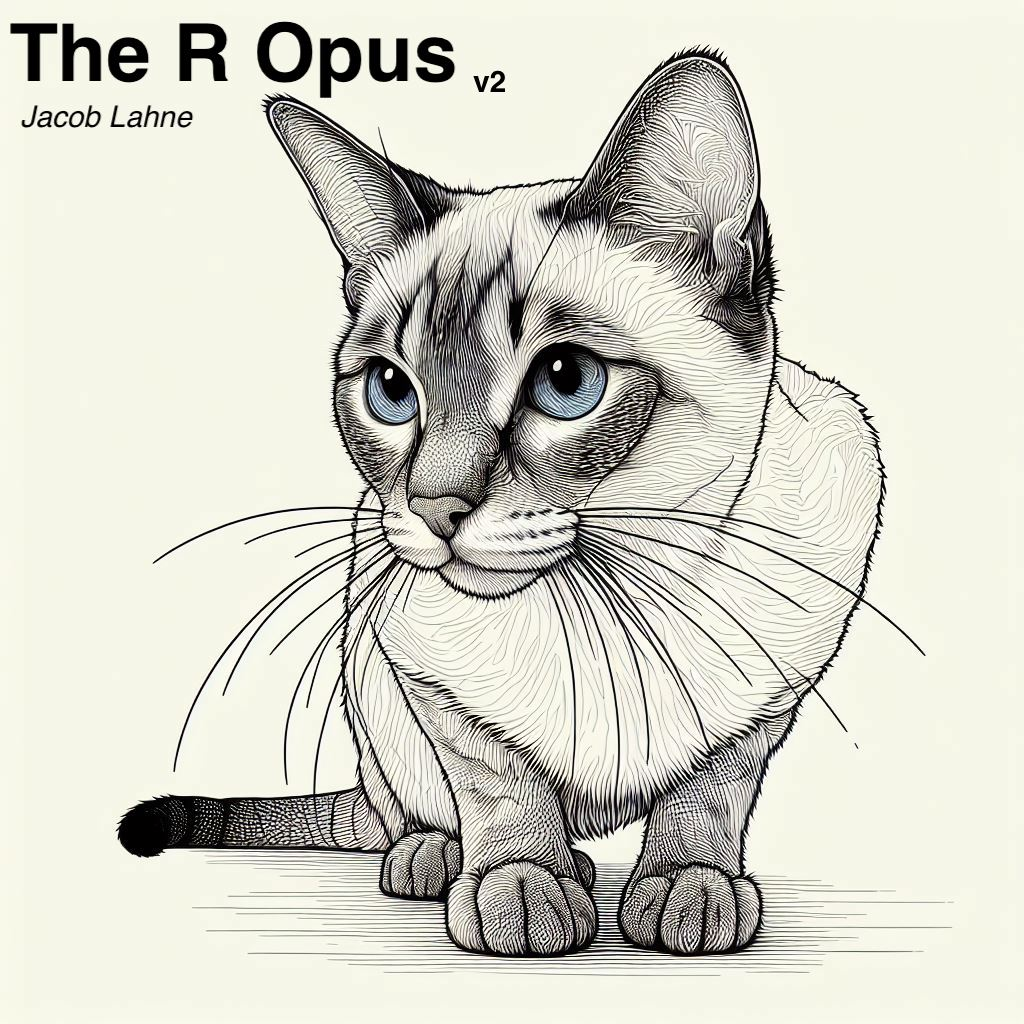
\includegraphics{img/r-opus-cover} \end{center}

To paraphrase one of my \href{https://bookdown.org/content/3890/}{inspirations for this project} \citep{kurzDoingBayesianDataAnalysis2023}: This is a labor of love. In 2015, \href{https://wineserver.ucdavis.edu/people/hildegarde-heymann\#/}{Hildegarde Heymann} (from here on: HGH), Distinguished Professor of Viticulture \& Enology at UC-Davis, was kind enough to host me as a visiting scholar at her laboratory. Among many other formative experiences I had as a sensory scientist at UC-Davis, HGH shared with me the \href{files/The\%20R\%20Opus\%20-\%20May\%202015.pdf}{\textbf{R Opus}}, a handbook she had written and compiled of common analytical approaches to multivariate (food-sensory) data in \texttt{R}. Like many of her other mentees, students, and postdocs, I benefited immensely from HGH's practical insight into how to apply abstruse multivariate analyses to real problems in research, and the \textbf{R Opus} manifested that knowledge into a hands-on guide for how to implement those tools.

In the time since, I have passed on the \textbf{R Opus} to my own mentees, students, and postdocs. As \texttt{R} has continued to mature and become more accessible as a scripting language for data analysis--in particular, as \href{https://r4ds.hadley.nz/}{``tidy'' programming principles} have become more dominant--I have found myself also passing on my own set of tips and tricks for how to transform the tools found in the original \textbf{R Opus} into the current vernacular. I began teaching data analytics and coding for researchers using \texttt{R}, and after learning how to (clumsily) transform my course notes into accessible \textbf{\href{https://bookdown.org/yihui/bookdown/}{bookdowns}}, I thought: why not the \textbf{R Opus}?

This is that thought put into some sort of action. I hope it is useful for you.

\section*{Usage}\label{usage}
\addcontentsline{toc}{section}{Usage}

This \textbf{bookdown} is constructed around typical workflows and data analysis needs for \href{https://en.wikipedia.org/wiki/Sensory_analysis}{sensory scientists}. You know who you are.

For all others, this bookdown is a structured introduction to the analysis of multivariate data from a practical and applied perspective. Specifically, we investigate how to apply a series of common multivariate statistical analyses to a set of data derived from the tasting and rating of wines by both trained and untrained human subjects. I place almost all of the emphasis on ``how to'', and much less on the statistical theory behind these approaches. As I have spent longer and longer using the statistical tools sensory scientists commonly apply (and occasionally developing and adapting new ones), I have come to believe that it is much more important to think of statistical analyses as tools that we apply, rather than worrying about our complete abstract understanding. The latter, of course, is also extremely important, but cannot be built without any possibility of first understanding why we might choose a particular analysis, and what it will look like applied to a particular dataset.

Even if you do not work in the field of sensory science, I hope that these examples will prove useful and easily understandable. Plus: thinking about how wine tastes is interesting, especially when we combine it with complicated statistics!

\section*{\texorpdfstring{\texttt{R} Setup}{R Setup}}\label{r-setup}
\addcontentsline{toc}{section}{\texttt{R} Setup}

You can read this bookdown entirely online using the navigation panels. However, if you want to learn to use \texttt{R} to conduct analyses like these, I strongly suggest you follow along. You'll need to install \texttt{R} to do so. To install \texttt{R}, go to \url{https://cran.r-project.org/} and follow the appropriate instructions for your operating system.

While it is not strictly necessary, you will almost certainly find it more pleasant to use the RStudio IDE (Interactive Development Environment) for \texttt{R}, which can be downloaded and installed from \url{https://posit.co/products/open-source/rstudio/}.

Here's the list of packages I used in this bookdown:

\begin{tabular}{l}
\hline
package\\
\hline
tidyverse\\
\hline
FactoMineR\\
\hline
patchwork\\
\hline
ggrepel\\
\hline
ggedit\\
\hline
ggforce\\
\hline
DistatisR\\
\hline
SensoMineR\\
\hline
paletteer\\
\hline
here\\
\hline
broom\\
\hline
skimr\\
\hline
factoextra\\
\hline
naniar\\
\hline
agricolae\\
\hline
tidytext\\
\hline
brms\\
\hline
tidybayes\\
\hline
simputation\\
\hline
missMDA\\
\hline
corrr\\
\hline
widyr\\
\hline
rgl\\
\hline
candisc\\
\hline
MASS\\
\hline
ca\\
\hline
pls\\
\hline
\end{tabular}

Once you have set up \texttt{R} (and RStudio), you can run the following lines of code to install the packages I use in this bookdown. This might take a minute--and you might have to restart \texttt{R} to do it. Go get a snack!

\begin{Shaded}
\begin{Highlighting}[]
\NormalTok{packages }\OtherTok{\textless{}{-}} \FunctionTok{c}\NormalTok{(}\StringTok{"tidyverse"}\NormalTok{, }\StringTok{"FactoMineR"}\NormalTok{, }\StringTok{"patchwork"}\NormalTok{, }\StringTok{"ggrepel"}\NormalTok{, }\StringTok{"ggedit"}\NormalTok{, }\StringTok{"ggforce"}\NormalTok{, }\StringTok{"DistatisR"}\NormalTok{, }\StringTok{"SensoMineR"}\NormalTok{, }\StringTok{"paletteer"}\NormalTok{, }\StringTok{"here"}\NormalTok{, }\StringTok{"broom"}\NormalTok{, }\StringTok{"skimr"}\NormalTok{, }\StringTok{"factoextra"}\NormalTok{, }\StringTok{"naniar"}\NormalTok{, }\StringTok{"agricolae"}\NormalTok{, }\StringTok{"tidytext"}\NormalTok{, }\StringTok{"brms"}\NormalTok{, }\StringTok{"tidybayes"}\NormalTok{, }\StringTok{"simputation"}\NormalTok{, }\StringTok{"missMDA"}\NormalTok{, }\StringTok{"corrr"}\NormalTok{, }\StringTok{"widyr"}\NormalTok{, }\StringTok{"rgl"}\NormalTok{, }\StringTok{"candisc"}\NormalTok{, }\StringTok{"MASS"}\NormalTok{, }\StringTok{"ca"}\NormalTok{, }\StringTok{"pls"}\NormalTok{)}

\FunctionTok{install.packages}\NormalTok{(packages, }\AttributeTok{dependencies =} \ConstantTok{TRUE}\NormalTok{)}
\end{Highlighting}
\end{Shaded}

Some of these tools install some additional (extra-\texttt{R}) tools. The Stan-based tools are most likely to cause trouble. If you cannot install them, consider the \href{https://mc-stan.org/users/interfaces/}{walkthroughs on the main Stan website}. Not installing them means you just won't be able to replicate my extended experiments with Bayesian modeling (probably not the greatest loss in the world for you).

\section*{What this is not}\label{what-this-is-not}
\addcontentsline{toc}{section}{What this is not}

I will not be going over the basics of \texttt{R} coding and programming. You can pick up a a fair amount by following along, or if you are truly new to \texttt{R} I recommend checking out \href{https://r4ds.hadley.nz/}{Wickham et al's now-classic introduction}, the \href{https://stat545.com/}{Stat545 website}, or any of the \href{https://datacarpentry.org/r-socialsci/}{Carpentries workshops}.

\section*{About me}\label{about-me}
\addcontentsline{toc}{section}{About me}

I'm an \href{https://www.fst.vt.edu/aboutus/faculty/jlahne.html}{associate professor of Food Science \& Technology at Virginia Tech}. I teach about sensory evaluation and about applied data analysis for food and ag scientists. I am not a statistician, but I interact with and consume a lot of statistics.

\begin{center}\rule{0.5\linewidth}{0.5pt}\end{center}

\section*{Changelog}\label{changelog}
\addcontentsline{toc}{section}{Changelog}

\subsection*{v0.2 (December 2024)}\label{v0.2-december-2024}
\addcontentsline{toc}{subsection}{v0.2 (December 2024)}

Update to fix typos, inconsistencies, and for use as ``textbook'' for FST 5984 (Spring 2025).

\subsection*{v0.1 (December 2023)}\label{v0.1-december-2023}
\addcontentsline{toc}{subsection}{v0.1 (December 2023)}

Initial commit. Everything works. There are typos and sections that need to be expanded (hi, Preference Mapping!).

\begin{center}\rule{0.5\linewidth}{0.5pt}\end{center}

\section*{Session Info}\label{session-info}
\addcontentsline{toc}{section}{Session Info}

At the end of chapter, I will be including a \texttt{sessionInfo()} chunk to try to make it easier to reproduce the work, as well as to diagnose any problems.

\begin{Shaded}
\begin{Highlighting}[]
\FunctionTok{sessionInfo}\NormalTok{()}
\CommentTok{\#\textgreater{} R version 4.4.1 (2024{-}06{-}14)}
\CommentTok{\#\textgreater{} Platform: x86\_64{-}apple{-}darwin20}
\CommentTok{\#\textgreater{} Running under: macOS 15.2}
\CommentTok{\#\textgreater{} }
\CommentTok{\#\textgreater{} Matrix products: default}
\CommentTok{\#\textgreater{} BLAS:   /Library/Frameworks/R.framework/Versions/4.4{-}x86\_64/Resources/lib/libRblas.0.dylib }
\CommentTok{\#\textgreater{} LAPACK: /Library/Frameworks/R.framework/Versions/4.4{-}x86\_64/Resources/lib/libRlapack.dylib;  LAPACK version 3.12.0}
\CommentTok{\#\textgreater{} }
\CommentTok{\#\textgreater{} locale:}
\CommentTok{\#\textgreater{} [1] en\_US.UTF{-}8/en\_US.UTF{-}8/en\_US.UTF{-}8/C/en\_US.UTF{-}8/en\_US.UTF{-}8}
\CommentTok{\#\textgreater{} }
\CommentTok{\#\textgreater{} time zone: America/New\_York}
\CommentTok{\#\textgreater{} tzcode source: internal}
\CommentTok{\#\textgreater{} }
\CommentTok{\#\textgreater{} attached base packages:}
\CommentTok{\#\textgreater{} [1] stats     graphics  grDevices datasets  utils    }
\CommentTok{\#\textgreater{} [6] methods   base     }
\CommentTok{\#\textgreater{} }
\CommentTok{\#\textgreater{} other attached packages:}
\CommentTok{\#\textgreater{}  [1] lubridate\_1.9.3 forcats\_1.0.0   stringr\_1.5.1  }
\CommentTok{\#\textgreater{}  [4] dplyr\_1.1.4     purrr\_1.0.2     readr\_2.1.5    }
\CommentTok{\#\textgreater{}  [7] tidyr\_1.3.1     tibble\_3.2.1    ggplot2\_3.5.1  }
\CommentTok{\#\textgreater{} [10] tidyverse\_2.0.0}
\CommentTok{\#\textgreater{} }
\CommentTok{\#\textgreater{} loaded via a namespace (and not attached):}
\CommentTok{\#\textgreater{}  [1] gtable\_0.3.5      compiler\_4.4.1    renv\_1.0.9       }
\CommentTok{\#\textgreater{}  [4] tidyselect\_1.2.1  scales\_1.3.0      yaml\_2.3.8       }
\CommentTok{\#\textgreater{}  [7] fastmap\_1.2.0     R6\_2.5.1          generics\_0.1.3   }
\CommentTok{\#\textgreater{} [10] knitr\_1.46        bookdown\_0.39     munsell\_0.5.1    }
\CommentTok{\#\textgreater{} [13] pillar\_1.9.0      tzdb\_0.4.0        rlang\_1.1.4      }
\CommentTok{\#\textgreater{} [16] utf8\_1.2.4        stringi\_1.8.4     xfun\_0.49        }
\CommentTok{\#\textgreater{} [19] timechange\_0.3.0  cli\_3.6.3         withr\_3.0.0      }
\CommentTok{\#\textgreater{} [22] magrittr\_2.0.3    digest\_0.6.37     grid\_4.4.1       }
\CommentTok{\#\textgreater{} [25] rstudioapi\_0.16.0 hms\_1.1.3         lifecycle\_1.0.4  }
\CommentTok{\#\textgreater{} [28] vctrs\_0.6.5       evaluate\_0.23     glue\_1.7.0       }
\CommentTok{\#\textgreater{} [31] fansi\_1.0.6       colorspace\_2.1{-}0  rmarkdown\_2.27   }
\CommentTok{\#\textgreater{} [34] tools\_4.4.1       pkgconfig\_2.0.3   htmltools\_0.5.8.1}
\end{Highlighting}
\end{Shaded}

\chapter{Data import and set up}\label{data-import-and-set-up}

In the original \textbf{R Opus}, HGH presented datasets from actual research conducted in her lab, that she worked with throughout. I think this is a great approach, and with her permission we're going to replicate her work, almost step for step, on the same datasets. Here, we'll review how to get them loaded and familiarize ourselves with them.

\section{Exploring our data}\label{exploring-our-data}

Most of the \textbf{R Opus} concerns 4 datasets. Let's import them and inspect them. We're going to use the \texttt{tidyverse} set of packages for basic data import and wrangling.

\begin{Shaded}
\begin{Highlighting}[]
\FunctionTok{library}\NormalTok{(tidyverse)}
\FunctionTok{library}\NormalTok{(here) }\CommentTok{\# easy file navigation}

\NormalTok{descriptive\_data }\OtherTok{\textless{}{-}} \FunctionTok{read\_csv}\NormalTok{(}\FunctionTok{here}\NormalTok{(}\StringTok{"data/torriDAFinal.csv"}\NormalTok{))}
\NormalTok{consumer\_data }\OtherTok{\textless{}{-}} \FunctionTok{read\_csv}\NormalTok{(}\FunctionTok{here}\NormalTok{(}\StringTok{"data/torriconsFinal.csv"}\NormalTok{))}
\NormalTok{sorting\_data }\OtherTok{\textless{}{-}} \FunctionTok{read\_csv}\NormalTok{(}\FunctionTok{here}\NormalTok{(}\StringTok{"data/sorting\_r1.csv"}\NormalTok{))}
\NormalTok{missing\_data\_example }\OtherTok{\textless{}{-}}\FunctionTok{read\_csv}\NormalTok{(}\FunctionTok{here}\NormalTok{(}\StringTok{"data/torrimiss.csv"}\NormalTok{))}
\end{Highlighting}
\end{Shaded}

We've now created four data tables (called ``tibbles'' in the \texttt{tidyverse} parlance) with our data, which you can see in your \texttt{Environment}. Let's look at each of these.

\subsection{The descriptive data}\label{the-descriptive-data}

\begin{Shaded}
\begin{Highlighting}[]
\FunctionTok{glimpse}\NormalTok{(descriptive\_data)}
\end{Highlighting}
\end{Shaded}

\begin{verbatim}
## Rows: 336
## Columns: 23
## $ NJ              <dbl> 1331, 1331, 1331, 1331, 1331, 1331, 1331, 1331, 1400, ~
## $ ProductName     <chr> "C_MERLOT", "C_SYRAH", "C_ZINFANDEL", "C_REFOSCO", "I_~
## $ NR              <dbl> 7, 7, 7, 7, 7, 7, 7, 7, 7, 7, 7, 7, 7, 7, 7, 7, 7, 7, ~
## $ Red_berry       <dbl> 5.1, 5.6, 4.9, 5.0, 3.3, 5.7, 2.9, 3.2, 0.1, 1.6, 4.5,~
## $ Dark_berry      <dbl> 5.8, 1.9, 2.6, 1.9, 7.2, 3.6, 5.1, 6.0, 0.1, 0.7, 2.9,~
## $ Jam             <dbl> 2.1, 3.9, 1.4, 7.8, 0.5, 8.7, 8.7, 4.0, 0.2, 0.0, 0.3,~
## $ Dried_fruit     <dbl> 4.7, 1.2, 5.9, 0.6, 5.8, 1.9, 0.4, 0.7, 2.9, 6.4, 2.4,~
## $ Artificial_frui <dbl> 1.0, 7.9, 0.8, 6.6, 0.7, 7.4, 6.2, 4.1, 0.1, 0.1, 0.1,~
## $ Chocolate       <dbl> 2.9, 1.0, 2.0, 6.4, 2.1, 3.3, 3.4, 3.6, 0.2, 1.0, 0.2,~
## $ Vanilla         <dbl> 5.0, 8.3, 2.7, 5.5, 1.3, 6.9, 8.1, 4.8, 2.0, 0.8, 1.9,~
## $ Oak             <dbl> 5.0, 2.3, 5.6, 3.6, 2.1, 1.5, 1.8, 2.6, 3.0, 5.4, 6.1,~
## $ Burned          <dbl> 1.4, 1.8, 1.9, 3.2, 5.6, 0.2, 0.4, 4.7, 7.5, 5.1, 0.3,~
## $ Leather         <dbl> 2.3, 3.5, 4.3, 0.3, 6.5, 1.5, 4.1, 6.5, 0.7, 0.8, 0.2,~
## $ Earthy          <dbl> 0.6, 1.0, 0.6, 0.2, 4.7, 0.3, 0.5, 1.9, 0.7, 3.0, 1.3,~
## $ Spicy           <dbl> 3.2, 0.7, 1.4, 2.9, 0.7, 3.1, 0.7, 1.4, 0.3, 3.2, 3.1,~
## $ Pepper          <dbl> 5.4, 3.0, 4.1, 0.9, 2.8, 1.6, 3.6, 4.5, 0.1, 2.0, 0.9,~
## $ Grassy          <dbl> 2.1, 0.6, 3.6, 1.8, 3.8, 0.9, 2.3, 0.8, 0.1, 1.3, 0.4,~
## $ Medicinal       <dbl> 0.4, 2.2, 1.7, 0.2, 2.6, 0.5, 0.2, 3.8, 0.1, 2.1, 0.1,~
## $ `Band-aid`      <dbl> 0.4, 0.4, 0.1, 0.2, 5.1, 1.2, 0.2, 6.2, 0.1, 1.1, 0.1,~
## $ Sour            <dbl> 5.0, 9.7, 7.8, 8.3, 7.6, 7.2, 5.9, 6.3, 5.7, 6.4, 5.4,~
## $ Bitter          <dbl> 5.9, 5.2, 3.5, 3.0, 1.9, 9.8, 2.9, 0.2, 0.6, 2.9, 0.1,~
## $ Alcohol         <dbl> 9.0, 7.2, 4.7, 8.9, 2.8, 8.7, 1.6, 7.0, 1.6, 5.4, 4.9,~
## $ Astringent      <dbl> 8.7, 8.3, 5.0, 7.8, 5.9, 8.0, 2.6, 4.2, 5.5, 5.1, 5.9,~
\end{verbatim}

The \texttt{descriptive\_data} file, read from \texttt{torriDAFinal.csv}, contains results from a descriptive analysis (DA) of wines, I believe from California and Italy (more on that in a minute). Each row contains the observation of multiple variables (columns) from a single judge (\texttt{NJ}) on a single wine (\texttt{ProductName}) in a single replicate (\texttt{NR}). That means we have 20 measured, quantitative sensory variables (\texttt{Red\_berry:Astringent}), and the other three variables (judge, wine, rep) are ID or classifying variables. \href{https://r4ds.hadley.nz/data-tidy.html}{These data are \emph{not} tidy}; each row has multiple variables.

We can learn a little more about these data before we move on: let's figure out how many samples, how many judges, and how many reps we have:

\begin{Shaded}
\begin{Highlighting}[]
\CommentTok{\# There are 14 judges, each of whom completed the same number of observations}
\NormalTok{descriptive\_data }\SpecialCharTok{\%\textgreater{}\%}
  \FunctionTok{count}\NormalTok{(NJ, }\AttributeTok{sort =} \ConstantTok{TRUE}\NormalTok{)}
\end{Highlighting}
\end{Shaded}

\begin{verbatim}
## # A tibble: 14 x 2
##       NJ     n
##    <dbl> <int>
##  1  1331    24
##  2  1400    24
##  3  1401    24
##  4  1402    24
##  5  1404    24
##  6  1405    24
##  7  1408    24
##  8  1409    24
##  9  1412    24
## 10  1413    24
## 11  1414    24
## 12  1415    24
## 13  1416    24
## 14  1417    24
\end{verbatim}

\begin{Shaded}
\begin{Highlighting}[]
\CommentTok{\# There are 3 reps (labeled as 7, 8, and 9), balanced}
\NormalTok{descriptive\_data }\SpecialCharTok{\%\textgreater{}\%}
  \FunctionTok{count}\NormalTok{(NR)}
\end{Highlighting}
\end{Shaded}

\begin{verbatim}
## # A tibble: 3 x 2
##      NR     n
##   <dbl> <int>
## 1     7   112
## 2     8   112
## 3     9   112
\end{verbatim}

\begin{Shaded}
\begin{Highlighting}[]
\CommentTok{\# There are 8 products, 4 from Italy and 4 from California}
\NormalTok{descriptive\_data }\SpecialCharTok{\%\textgreater{}\%}
  \FunctionTok{count}\NormalTok{(ProductName)}
\end{Highlighting}
\end{Shaded}

\begin{verbatim}
## # A tibble: 8 x 2
##   ProductName     n
##   <chr>       <int>
## 1 C_MERLOT       42
## 2 C_REFOSCO      42
## 3 C_SYRAH        42
## 4 C_ZINFANDEL    42
## 5 I_MERLOT       42
## 6 I_PRIMITIVO    42
## 7 I_REFOSCO      42
## 8 I_SYRAH        42
\end{verbatim}

The \texttt{\%\textgreater{}\%} operator is called \textbf{the pipe}, and it takes whatever is on its left side and passes it on to the right side. You can learn more about the pipe, but you can also just experiment. When you see it in code, you can read it as ``\ldots and then\ldots{}'', so above we'd say something like ``take \texttt{descriptive\_data} \textbf{and then} count the number of times each \texttt{NJ} value occurs''. The other thing to know about piping, that you will see in some code in the \textbf{R Opus}, is the use of the period, \texttt{.}, as a ``pronoun'' for whatever is getting passed from the previous line. This lets you tell the pipe where in the line you want the output from the previous/left side to end up:

\begin{Shaded}
\begin{Highlighting}[]
 \CommentTok{\# Take the descriptive data}
\NormalTok{descriptive\_data }\SpecialCharTok{\%\textgreater{}\%}
\CommentTok{\# AND THEN run 1{-}way ANOVA, with descriptive\_data passed to the \textasciigrave{}data =\textasciigrave{} argument of aov()}
  \FunctionTok{aov}\NormalTok{(Jam }\SpecialCharTok{\textasciitilde{}}\NormalTok{ ProductName, }\AttributeTok{data =}\NormalTok{ .) }\SpecialCharTok{\%\textgreater{}\%}
\CommentTok{\# AND THEN print the readable summary of the results of aov()}
  \FunctionTok{summary}\NormalTok{()}
\end{Highlighting}
\end{Shaded}

\begin{verbatim}
##              Df Sum Sq Mean Sq F value   Pr(>F)    
## ProductName   7  280.6   40.08   7.882 7.74e-09 ***
## Residuals   328 1667.9    5.08                     
## ---
## Signif. codes:  0 '***' 0.001 '**' 0.01 '*' 0.05 '.' 0.1 ' ' 1
\end{verbatim}

Turns out that \texttt{Jam} attribute might vary by product. We'll see.

\subsection{Consumer data}\label{consumer-data}

Let's look at the data in \texttt{consumer\_data}:

\begin{Shaded}
\begin{Highlighting}[]
\FunctionTok{glimpse}\NormalTok{(consumer\_data)}
\end{Highlighting}
\end{Shaded}

\begin{verbatim}
## Rows: 106
## Columns: 13
## $ Judge            <dbl> 1, 2, 3, 4, 5, 6, 7, 8, 9, 10, 11, 12, 13, 14, 15, 16~
## $ `Wine Frequency` <dbl> 2, 3, 3, 3, 2, 3, 2, 2, 1, 2, 2, 2, 1, 1, 1, 4, 1, 1,~
## $ `IT frequency`   <dbl> 3, 4, 1, 2, 3, 3, 4, 3, 3, 4, 3, 3, 3, 3, 3, 1, 3, 4,~
## $ Gender           <dbl> 2, 2, 1, 2, 1, 1, 2, 1, 1, 2, 1, 2, 1, 2, 1, 2, 2, 2,~
## $ Age              <dbl> 22, 21, 25, 24, 31, 60, 24, 25, 26, 40, 40, 22, 23, 2~
## $ C_MERLOT         <dbl> 5, 8, 8, 4, 4, 4, 8, 5, 7, 7, 7, 8, 6, 4, 4, 2, 3, 7,~
## $ C_SYRAH          <dbl> 4, 5, 6, 6, 6, 4, 6, 4, 5, 1, 8, 8, 4, 2, 4, 1, 8, 6,~
## $ C_ZINFANDEL      <dbl> 3, 8, 6, 3, 6, 4, 7, 6, 6, 4, 6, 7, 6, 8, 6, 7, 9, 7,~
## $ C_REFOSCO        <dbl> 8, 5, 8, 4, 7, 4, 6, 6, 3, 6, 3, 7, 8, 4, 6, 1, 8, 8,~
## $ I_MERLOT         <dbl> 7, 4, 7, 8, 2, 3, 8, 7, 6, 5, 3, 3, 3, 3, 4, 1, 6, 7,~
## $ I_SYRAH          <dbl> 2, 8, 5, 4, 6, 3, 6, 4, 6, 8, 2, 4, 8, 7, 3, 4, 4, 8,~
## $ I_PRIMITIVO      <dbl> 4, 4, 7, 9, 5, 4, 4, 4, 6, 1, 1, 2, 7, 3, 4, 2, 7, 6,~
## $ I_REFOSCO        <dbl> 6, 6, 7, 2, 7, 1, 7, 3, 3, 2, 4, 3, 7, 5, 4, 4, 6, 7,~
\end{verbatim}

Here we have consumer acceptance testing data on the same 8 wines from the DA. The rows look like they represent consumers, identified by the \texttt{Judge} column. Let's check to see if they're all unique:

\begin{Shaded}
\begin{Highlighting}[]
\NormalTok{consumer\_data }\SpecialCharTok{\%\textgreater{}\%}
\CommentTok{\# The sort = TRUE argument would put anyone with multiple rows at the top}
  \FunctionTok{count}\NormalTok{(Judge, }\AttributeTok{sort =} \ConstantTok{TRUE}\NormalTok{)}
\end{Highlighting}
\end{Shaded}

\begin{verbatim}
## # A tibble: 106 x 2
##    Judge     n
##    <dbl> <int>
##  1     1     1
##  2     2     1
##  3     3     1
##  4     4     1
##  5     5     1
##  6     6     1
##  7     7     1
##  8     8     1
##  9     9     1
## 10    10     1
## # i 96 more rows
\end{verbatim}

Then we have some consumption data (\texttt{Wine\ Frequency} and \texttt{IT\ Frequency}) and some demographic data (\texttt{Gender} and \texttt{Age}), and then 8 columns representing each judge's rating for each wine. Doesn't look like we have any replication or any incomplete data. Again, this is not tidy data--each row contains multiple observations beyond the classifying/identifying data. We'll come back to that.

\subsection{The other data frames}\label{the-other-data-frames}

The other two data frames we're going to pay less attention to for now. The first, \texttt{missing\_data\_example}, is the same data frame as \texttt{descriptive\_data} but with missing data introduced on purpose for didactic purposes. We can use the \texttt{naniar} package to quickly learn a litle bit about the missingness:

\begin{Shaded}
\begin{Highlighting}[]
\FunctionTok{library}\NormalTok{(naniar)}

\NormalTok{naniar}\SpecialCharTok{::}\FunctionTok{gg\_miss\_var}\NormalTok{(}\AttributeTok{x =}\NormalTok{ missing\_data\_example)}
\end{Highlighting}
\end{Shaded}

\pandocbounded{\includegraphics[keepaspectratio]{01-data-wrangling_files/figure-latex/unnamed-chunk-7-1.pdf}}

We could also use the useful \texttt{skimr} package to give us an informative data summary that would tell us about missingness:

\begin{Shaded}
\begin{Highlighting}[]
\FunctionTok{library}\NormalTok{(skimr)}
\end{Highlighting}
\end{Shaded}

\begin{verbatim}
## 
## Attaching package: 'skimr'
\end{verbatim}

\begin{verbatim}
## The following object is masked from 'package:naniar':
## 
##     n_complete
\end{verbatim}

\begin{Shaded}
\begin{Highlighting}[]
\FunctionTok{skim}\NormalTok{(missing\_data\_example) }\SpecialCharTok{\%\textgreater{}\%} 
  \CommentTok{\# This is purely to allow the skimr::skim() to be rendered in PDF, ignore otherwise}
\NormalTok{  knitr}\SpecialCharTok{::}\FunctionTok{kable}\NormalTok{()}
\end{Highlighting}
\end{Shaded}

\begin{tabular}{l|l|r|r|r|r|r|r|r|r|r|r|r|r|r|r|l}
\hline
skim\_type & skim\_variable & n\_missing & complete\_rate & character.min & character.max & character.empty & character.n\_unique & character.whitespace & numeric.mean & numeric.sd & numeric.p0 & numeric.p25 & numeric.p50 & numeric.p75 & numeric.p100 & numeric.hist\\
\hline
character & ProductName & 0 & 1.0000000 & 7 & 11 & 0 & 8 & 0 & NA & NA & NA & NA & NA & NA & NA & NA\\
\hline
numeric & NJ & 0 & 1.0000000 & NA & NA & NA & NA & NA & 1403.3571429 & 20.8589537 & 1331 & 1402.000 & 1408.50 & 1414.000 & 1417.0 & ▁▁▁▁▇\\
\hline
numeric & NR & 0 & 1.0000000 & NA & NA & NA & NA & NA & 8.0000000 & 0.8177143 & 7 & 7.000 & 8.00 & 9.000 & 9.0 & ▇▁▇▁▇\\
\hline
numeric & Red\_berry & 11 & 0.9672619 & NA & NA & NA & NA & NA & 2.8473846 & 2.5294746 & 0 & 0.500 & 2.30 & 4.800 & 9.2 & ▇▅▂▂▁\\
\hline
numeric & Dark\_berry & 10 & 0.9702381 & NA & NA & NA & NA & NA & 3.0953988 & 2.7778038 & 0 & 0.500 & 2.30 & 5.075 & 9.9 & ▇▃▃▂▂\\
\hline
numeric & Jam & 10 & 0.9702381 & NA & NA & NA & NA & NA & 1.8773006 & 2.4022502 & 0 & 0.200 & 0.70 & 2.700 & 10.0 & ▇▂▁▁▁\\
\hline
numeric & Dried\_fruit & 10 & 0.9702381 & NA & NA & NA & NA & NA & 1.8104294 & 2.1395934 & 0 & 0.200 & 0.70 & 3.275 & 10.0 & ▇▂▂▁▁\\
\hline
numeric & Artificial\_frui & 10 & 0.9702381 & NA & NA & NA & NA & NA & 1.1996933 & 1.9710598 & 0 & 0.100 & 0.30 & 1.200 & 9.7 & ▇▁▁▁▁\\
\hline
numeric & Chocolate & 10 & 0.9702381 & NA & NA & NA & NA & NA & 1.2131902 & 1.7648302 & 0 & 0.100 & 0.40 & 1.675 & 10.0 & ▇▁▁▁▁\\
\hline
numeric & Vanilla & 11 & 0.9672619 & NA & NA & NA & NA & NA & 1.6673846 & 1.9758529 & 0 & 0.200 & 0.90 & 2.600 & 9.3 & ▇▂▁▁▁\\
\hline
numeric & Oak & 10 & 0.9702381 & NA & NA & NA & NA & NA & 2.3024540 & 1.9957632 & 0 & 0.500 & 1.70 & 3.900 & 9.0 & ▇▃▃▁▁\\
\hline
numeric & Burned & 10 & 0.9702381 & NA & NA & NA & NA & NA & 1.5070552 & 2.0622868 & 0 & 0.100 & 0.40 & 2.375 & 9.7 & ▇▂▁▁▁\\
\hline
numeric & Leather & 10 & 0.9702381 & NA & NA & NA & NA & NA & 1.4659509 & 2.0566530 & 0 & 0.100 & 0.40 & 2.400 & 9.9 & ▇▂▁▁▁\\
\hline
numeric & Earthy & 10 & 0.9702381 & NA & NA & NA & NA & NA & 1.0929448 & 1.5826888 & 0 & 0.100 & 0.40 & 1.375 & 8.0 & ▇▁▁▁▁\\
\hline
numeric & Spicy & 10 & 0.9702381 & NA & NA & NA & NA & NA & 1.2015337 & 1.6742477 & 0 & 0.100 & 0.40 & 1.800 & 8.9 & ▇▂▁▁▁\\
\hline
numeric & Pepper & 10 & 0.9702381 & NA & NA & NA & NA & NA & 1.5165644 & 2.0514989 & 0 & 0.200 & 0.50 & 2.300 & 10.0 & ▇▁▁▁▁\\
\hline
numeric & Grassy & 10 & 0.9702381 & NA & NA & NA & NA & NA & 0.9361963 & 1.4584638 & 0 & 0.100 & 0.30 & 1.100 & 9.8 & ▇▁▁▁▁\\
\hline
numeric & Medicinal & 10 & 0.9702381 & NA & NA & NA & NA & NA & 1.4276074 & 2.0269504 & 0 & 0.100 & 0.40 & 2.000 & 9.6 & ▇▁▁▁▁\\
\hline
numeric & Band-aid & 10 & 0.9702381 & NA & NA & NA & NA & NA & 1.2061350 & 2.0478189 & 0 & 0.100 & 0.30 & 1.075 & 9.8 & ▇▁▁▁▁\\
\hline
numeric & Sour & 10 & 0.9702381 & NA & NA & NA & NA & NA & 4.6199387 & 2.9908889 & 0 & 1.625 & 4.85 & 7.100 & 10.0 & ▇▅▇▆▅\\
\hline
numeric & Bitter & 10 & 0.9702381 & NA & NA & NA & NA & NA & 3.4236196 & 2.7514405 & 0 & 1.000 & 3.00 & 5.200 & 10.0 & ▇▅▃▂▂\\
\hline
numeric & Alcohol & 10 & 0.9702381 & NA & NA & NA & NA & NA & 3.6058282 & 2.4028950 & 0 & 1.200 & 4.05 & 5.200 & 9.5 & ▇▃▇▃▁\\
\hline
numeric & Astringent & 10 & 0.9702381 & NA & NA & NA & NA & NA & 4.6358896 & 2.6451989 & 0 & 2.500 & 4.70 & 6.400 & 10.0 & ▆▆▇▅▃\\
\hline
\end{tabular}

Because the only difference between this data table and the \texttt{descriptive\_data} table is the introduced missingness we're not going to pay much attention to it until we get to dealing with missing data.

The \texttt{sorting\_data} data frame contains results from a sorting task in which 15 subjects (1 per column) sorted the same wines into disjoint groups according to their own criteria. If in a column two wines have the same label (say, \texttt{G1}), that subject put them in the same group. We'll get to how to deal with this kind of data later on, so we're not going to go into more depth here.

\begin{Shaded}
\begin{Highlighting}[]
\NormalTok{sorting\_data}
\end{Highlighting}
\end{Shaded}

\begin{verbatim}
## # A tibble: 8 x 16
##   wine      `263` `1331` `1400` `1401` `1402` `1404` `1405` `1408` `1409` `1412`
##   <chr>     <chr> <chr>  <chr>  <chr>  <chr>  <chr>  <chr>  <chr>  <chr>  <chr> 
## 1 I_REFOSCO G6    G3     G5     G4     G5     G4     G2     G2     G1     G1    
## 2 I_MERLOT  G1    G3     G4     G3     G2     G3     G4     G3     G1     G2    
## 3 I_SYRAH   G5    G4     G2     G1     G1     G2     G1     G4     G1     G2    
## 4 I_PRIMIT~ G2    G1     G3     G1     G4     G5     G3     G4     G3     G2    
## 5 C_SYRAH   G3    G2     G4     G4     G5     G6     G1     G3     G2     G4    
## 6 C_REFOSCO G4    G3     G1     G2     G5     G5     G2     G1     G2     G3    
## 7 C_MERLOT  G1    G2     G3     G3     G3     G1     G4     G3     G2     G2    
## 8 C_ZINFAN~ G1    G5     G3     G3     G2     G1     G1     G3     G1     G2    
## # i 5 more variables: `1413` <chr>, `1414` <chr>, `1415` <chr>, `1416` <chr>,
## #   `1417` <chr>
\end{verbatim}

\section{Wrangling/tidying data}\label{wranglingtidying-data}

Whenever we do data analysis, about 90\% of the effort is getting the data into the right shape for the analysis at hand. We're going to be employing many approaches to this task throughout the \textbf{R Opus}, but here we'll do a quick preparatory analysis with our two untidy data frames.

The \texttt{pivot\_longer()} function in \texttt{dplyr} is built to take data in the many-observations-per-row format (often called ``wide'' data) and bring it into a longer, ``tidier'' representation that is often easier to work with. For the \texttt{descriptive\_data}, a natural format that would be easier to work with is one in which all the descriptors are pivoted into two columns: one labeling the descriptor by name, and the other giving the rated value. We'd do that as follows:

\begin{Shaded}
\begin{Highlighting}[]
\NormalTok{descriptive\_data\_tidy }\OtherTok{\textless{}{-}} 
\NormalTok{  descriptive\_data }\SpecialCharTok{\%\textgreater{}\%}
  \FunctionTok{pivot\_longer}\NormalTok{(}\AttributeTok{cols =} \SpecialCharTok{{-}}\FunctionTok{c}\NormalTok{(NJ, NR, ProductName),}
               \AttributeTok{names\_to =} \StringTok{"descriptor"}\NormalTok{,}
               \AttributeTok{values\_to =} \StringTok{"rating"}\NormalTok{)}

\NormalTok{descriptive\_data\_tidy}
\end{Highlighting}
\end{Shaded}

\begin{verbatim}
## # A tibble: 6,720 x 5
##       NJ ProductName    NR descriptor      rating
##    <dbl> <chr>       <dbl> <chr>            <dbl>
##  1  1331 C_MERLOT        7 Red_berry          5.1
##  2  1331 C_MERLOT        7 Dark_berry         5.8
##  3  1331 C_MERLOT        7 Jam                2.1
##  4  1331 C_MERLOT        7 Dried_fruit        4.7
##  5  1331 C_MERLOT        7 Artificial_frui    1  
##  6  1331 C_MERLOT        7 Chocolate          2.9
##  7  1331 C_MERLOT        7 Vanilla            5  
##  8  1331 C_MERLOT        7 Oak                5  
##  9  1331 C_MERLOT        7 Burned             1.4
## 10  1331 C_MERLOT        7 Leather            2.3
## # i 6,710 more rows
\end{verbatim}

Now we have kept our 3 ID or classifying variables and created a 4th, \texttt{descriptor}, which together uniquely describe each numeric observation, now called \texttt{rating}. In our newly tidied dataset, the first line give the \texttt{rating}--the observation--for the judge with code \texttt{1331}, in rep \texttt{7}, for the wine \texttt{C\_MERLOT}, for the \texttt{Red\_berry} descriptor. It's \texttt{5.1}.

To motivate this kind of work, let's quickly talk about the ``\href{https://www.jstatsoft.org/article/view/v040i01}{split-apply-combine}'' workflow this enables. Now that we've separated out our classifying variables, we can do work with them much more easily. For example, let's say we want to generate a means table comparing the wines on the \texttt{Jam} variable, which we know from our example above seems to vary per wine. We can now do this very easily:

\begin{Shaded}
\begin{Highlighting}[]
\NormalTok{descriptive\_data\_tidy }\SpecialCharTok{\%\textgreater{}\%}

\CommentTok{\# First we will use filter() to get only Jam observations}
  
  \FunctionTok{filter}\NormalTok{(descriptor }\SpecialCharTok{==} \StringTok{"Jam"}\NormalTok{) }\SpecialCharTok{\%\textgreater{}\%}
  
\CommentTok{\# Then we will use group\_by() to identify our wines as the relevant classifying variable}
  
  \FunctionTok{group\_by}\NormalTok{(ProductName) }\SpecialCharTok{\%\textgreater{}\%}
  
\CommentTok{\# Finally, we\textquotesingle{}ll use the summarize() function to generate a quick per{-}wine summary}
  
  \FunctionTok{summarize}\NormalTok{(}\AttributeTok{mean\_jam\_score =} \FunctionTok{mean}\NormalTok{(rating),}
            \AttributeTok{se\_jam\_score =} \FunctionTok{sd}\NormalTok{(rating) }\SpecialCharTok{/} \FunctionTok{sqrt}\NormalTok{(}\FunctionTok{n}\NormalTok{()),}
            \AttributeTok{lower\_95 =}\NormalTok{ mean\_jam\_score }\SpecialCharTok{{-}} \FloatTok{1.96} \SpecialCharTok{*}\NormalTok{ se\_jam\_score,}
            \AttributeTok{upper\_95 =}\NormalTok{ mean\_jam\_score }\SpecialCharTok{+} \FloatTok{1.96} \SpecialCharTok{*}\NormalTok{ se\_jam\_score)}
\end{Highlighting}
\end{Shaded}

\begin{verbatim}
## # A tibble: 8 x 5
##   ProductName mean_jam_score se_jam_score lower_95 upper_95
##   <chr>                <dbl>        <dbl>    <dbl>    <dbl>
## 1 C_MERLOT             1.37         0.262    0.857     1.89
## 2 C_REFOSCO            1.03         0.238    0.565     1.50
## 3 C_SYRAH              1.75         0.378    1.00      2.49
## 4 C_ZINFANDEL          1.98         0.394    1.21      2.75
## 5 I_MERLOT             0.843        0.185    0.480     1.21
## 6 I_PRIMITIVO          3.61         0.475    2.68      4.54
## 7 I_REFOSCO            1.54         0.282    0.982     2.09
## 8 I_SYRAH              3.10         0.453    2.21      3.98
\end{verbatim}

Our use of all of the intermediate steps--filtering, grouping, summarizing--depends on us having gotten the data into a tidy format. This will sometimes \emph{not} work well--especially when we're looking at pairwise relationships like covariance or correlation--but it will often be a step in wrangling results.

We can do the same thing with our \texttt{consumer\_data}. In this case, we have 5 ID variables, and 8 observations, one for each wine. Let's do the same thing with pivot\_longer:

\begin{Shaded}
\begin{Highlighting}[]
\NormalTok{consumer\_data\_tidy }\OtherTok{\textless{}{-}} 
\NormalTok{  consumer\_data }\SpecialCharTok{\%\textgreater{}\%}
  
\CommentTok{\# We can use ":" to select a continuous range of columns}
  
  \FunctionTok{pivot\_longer}\NormalTok{(}\AttributeTok{cols =}\NormalTok{ C\_MERLOT}\SpecialCharTok{:}\NormalTok{I\_REFOSCO,}
               \AttributeTok{names\_to =} \StringTok{"wine"}\NormalTok{,}
               \AttributeTok{values\_to =} \StringTok{"rating"}\NormalTok{)}

\NormalTok{consumer\_data\_tidy}
\end{Highlighting}
\end{Shaded}

\begin{verbatim}
## # A tibble: 848 x 7
##    Judge `Wine Frequency` `IT frequency` Gender   Age wine        rating
##    <dbl>            <dbl>          <dbl>  <dbl> <dbl> <chr>        <dbl>
##  1     1                2              3      2    22 C_MERLOT         5
##  2     1                2              3      2    22 C_SYRAH          4
##  3     1                2              3      2    22 C_ZINFANDEL      3
##  4     1                2              3      2    22 C_REFOSCO        8
##  5     1                2              3      2    22 I_MERLOT         7
##  6     1                2              3      2    22 I_SYRAH          2
##  7     1                2              3      2    22 I_PRIMITIVO      4
##  8     1                2              3      2    22 I_REFOSCO        6
##  9     2                3              4      2    21 C_MERLOT         8
## 10     2                3              4      2    21 C_SYRAH          5
## # i 838 more rows
\end{verbatim}

Again, we've created a new ID/classifying column called \texttt{wine} and a new observation column called \texttt{rating}. Now the 6 ID columns uniquely specify an observation. Let's do something fun with this: is there a relationship between \texttt{Gender} and \texttt{rating}?

\begin{Shaded}
\begin{Highlighting}[]
\NormalTok{consumer\_data\_tidy }\SpecialCharTok{\%\textgreater{}\%}
  \FunctionTok{lm}\NormalTok{(rating }\SpecialCharTok{\textasciitilde{}}\NormalTok{ Gender, }\AttributeTok{data =}\NormalTok{ .) }\SpecialCharTok{\%\textgreater{}\%}
  \FunctionTok{summary}\NormalTok{()}
\end{Highlighting}
\end{Shaded}

\begin{verbatim}
## 
## Call:
## lm(formula = rating ~ Gender, data = .)
## 
## Residuals:
##     Min      1Q  Median      3Q     Max 
## -4.3137 -1.3137  0.6863  1.6863  3.7091 
## 
## Coefficients:
##             Estimate Std. Error t value Pr(>|t|)    
## (Intercept)  5.26809    0.21653  24.330   <2e-16 ***
## Gender       0.02282    0.13852   0.165    0.869    
## ---
## Signif. codes:  0 '***' 0.001 '**' 0.01 '*' 0.05 '.' 0.1 ' ' 1
## 
## Residual standard error: 2.015 on 846 degrees of freedom
## Multiple R-squared:  3.207e-05,  Adjusted R-squared:  -0.00115 
## F-statistic: 0.02713 on 1 and 846 DF,  p-value: 0.8692
\end{verbatim}

Looks like there isn't, which is probably evidence of good sampling--I can't think why there would be such a relationship.

\section{Wrap up and summary}\label{wrap-up-and-summary}

At this point, we've already done quite a bit of work. We've practiced importing and inspecting data, and gotten a bit of practice with tidying data and applying the split-apply-combine data analysis steps. We're going to be moving on to applying Analysis of Variance (ANOVA) to these data next.

\section{Packages used in this chapter}\label{packages-used-in-this-chapter}

\begin{Shaded}
\begin{Highlighting}[]
\FunctionTok{sessionInfo}\NormalTok{()}
\end{Highlighting}
\end{Shaded}

\begin{verbatim}
## R version 4.4.1 (2024-06-14)
## Platform: x86_64-apple-darwin20
## Running under: macOS 15.2
## 
## Matrix products: default
## BLAS:   /Library/Frameworks/R.framework/Versions/4.4-x86_64/Resources/lib/libRblas.0.dylib 
## LAPACK: /Library/Frameworks/R.framework/Versions/4.4-x86_64/Resources/lib/libRlapack.dylib;  LAPACK version 3.12.0
## 
## locale:
## [1] en_US.UTF-8/en_US.UTF-8/en_US.UTF-8/C/en_US.UTF-8/en_US.UTF-8
## 
## time zone: America/New_York
## tzcode source: internal
## 
## attached base packages:
## [1] stats     graphics  grDevices datasets  utils     methods   base     
## 
## other attached packages:
##  [1] skimr_2.1.5     naniar_1.1.0    here_1.0.1      lubridate_1.9.3
##  [5] forcats_1.0.0   stringr_1.5.1   dplyr_1.1.4     purrr_1.0.2    
##  [9] readr_2.1.5     tidyr_1.3.1     tibble_3.2.1    ggplot2_3.5.1  
## [13] tidyverse_2.0.0
## 
## loaded via a namespace (and not attached):
##  [1] utf8_1.2.4        generics_0.1.3    renv_1.0.9        stringi_1.8.4    
##  [5] hms_1.1.3         digest_0.6.37     magrittr_2.0.3    evaluate_0.23    
##  [9] grid_4.4.1        timechange_0.3.0  bookdown_0.39     fastmap_1.2.0    
## [13] jsonlite_1.8.8    rprojroot_2.0.4   fansi_1.0.6       scales_1.3.0     
## [17] cli_3.6.3         rlang_1.1.4       crayon_1.5.2      bit64_4.0.5      
## [21] munsell_0.5.1     base64enc_0.1-3   repr_1.1.7        withr_3.0.0      
## [25] yaml_2.3.8        tools_4.4.1       parallel_4.4.1    tzdb_0.4.0       
## [29] colorspace_2.1-0  vctrs_0.6.5       R6_2.5.1          lifecycle_1.0.4  
## [33] bit_4.0.5         vroom_1.6.5       pkgconfig_2.0.3   pillar_1.9.0     
## [37] gtable_0.3.5      glue_1.7.0        visdat_0.6.0      highr_0.10       
## [41] xfun_0.49         tidyselect_1.2.1  rstudioapi_0.16.0 knitr_1.46       
## [45] farver_2.1.2      htmltools_0.5.8.1 labeling_0.4.3    rmarkdown_2.27   
## [49] compiler_4.4.1
\end{verbatim}

\chapter{Analysis of Variance}\label{analysis-of-variance}

So far we've imported and inspected our data. In case that got left behind, let's do it again (as well as setting up the basic packages we're going to use).

\begin{Shaded}
\begin{Highlighting}[]
\FunctionTok{library}\NormalTok{(tidyverse)}
\FunctionTok{library}\NormalTok{(here)}

\NormalTok{descriptive\_data }\OtherTok{\textless{}{-}} \FunctionTok{read\_csv}\NormalTok{(}\FunctionTok{here}\NormalTok{(}\StringTok{"data/torriDAFinal.csv"}\NormalTok{))}
\NormalTok{consumer\_data }\OtherTok{\textless{}{-}} \FunctionTok{read\_csv}\NormalTok{(}\FunctionTok{here}\NormalTok{(}\StringTok{"data/torriconsFinal.csv"}\NormalTok{))}
\end{Highlighting}
\end{Shaded}

\section{Univariate analysis with the linear model}\label{univariate-analysis-with-the-linear-model}

In the original \textbf{R Opus}, HGH made sure that the classifying variables in the \texttt{descriptive\_data} were set to the \texttt{factor} data type. \href{https://notstatschat.tumblr.com/post/124987394001/stringsasfactors-sigh}{There is a \emph{looong} history of factors in \texttt{R}}, and you can get a better crash course than I am going to give in some introductory course like \href{https://stat545.com/factors-boss.html}{Stat545}. Suffice it to say here that the \texttt{factor} data type is a labeled integer, and that it \st{is} \emph{used to be} the default way that \texttt{R} imports strings. It has some desirable characteristics, but it can often be non-intuitive for those learning \texttt{R}. Much of base \texttt{R} has now evolved to silently handle \texttt{character} data as \texttt{factor} when necessary, so unless you're a hardcore \texttt{R} user you probably don't need to worry about this too much.

\emph{That being said}, let's take the opportunity to follow along with HGH's intentions in order to learn some more data wrangling. In this case, HGH says that the \texttt{NJ}, \texttt{NR}, and \texttt{ProductName} variables in \texttt{descriptive\_data} should be \texttt{factor} data type, so let's make it so (this is definitely a good idea for \texttt{NJ} and \texttt{NR}, which are stored as numerals, as otherwise \texttt{R} will treat them as continuous numeric variables).

\begin{Shaded}
\begin{Highlighting}[]
\NormalTok{descriptive\_data }\OtherTok{\textless{}{-}} 
\NormalTok{  descriptive\_data }\SpecialCharTok{\%\textgreater{}\%}
  \FunctionTok{mutate}\NormalTok{(}\AttributeTok{NJ =} \FunctionTok{as.factor}\NormalTok{(NJ),}
         \AttributeTok{NR =} \FunctionTok{as.factor}\NormalTok{(NR),}
         \AttributeTok{ProductName =} \FunctionTok{as.factor}\NormalTok{(ProductName))}

\FunctionTok{glimpse}\NormalTok{(descriptive\_data)}
\end{Highlighting}
\end{Shaded}

\begin{verbatim}
## Rows: 336
## Columns: 23
## $ NJ              <fct> 1331, 1331, 1331, 1331, 1331, 1331, 1331, 1331, 1400, ~
## $ ProductName     <fct> C_MERLOT, C_SYRAH, C_ZINFANDEL, C_REFOSCO, I_MERLOT, I~
## $ NR              <fct> 7, 7, 7, 7, 7, 7, 7, 7, 7, 7, 7, 7, 7, 7, 7, 7, 7, 7, ~
## $ Red_berry       <dbl> 5.1, 5.6, 4.9, 5.0, 3.3, 5.7, 2.9, 3.2, 0.1, 1.6, 4.5,~
## $ Dark_berry      <dbl> 5.8, 1.9, 2.6, 1.9, 7.2, 3.6, 5.1, 6.0, 0.1, 0.7, 2.9,~
## $ Jam             <dbl> 2.1, 3.9, 1.4, 7.8, 0.5, 8.7, 8.7, 4.0, 0.2, 0.0, 0.3,~
## $ Dried_fruit     <dbl> 4.7, 1.2, 5.9, 0.6, 5.8, 1.9, 0.4, 0.7, 2.9, 6.4, 2.4,~
## $ Artificial_frui <dbl> 1.0, 7.9, 0.8, 6.6, 0.7, 7.4, 6.2, 4.1, 0.1, 0.1, 0.1,~
## $ Chocolate       <dbl> 2.9, 1.0, 2.0, 6.4, 2.1, 3.3, 3.4, 3.6, 0.2, 1.0, 0.2,~
## $ Vanilla         <dbl> 5.0, 8.3, 2.7, 5.5, 1.3, 6.9, 8.1, 4.8, 2.0, 0.8, 1.9,~
## $ Oak             <dbl> 5.0, 2.3, 5.6, 3.6, 2.1, 1.5, 1.8, 2.6, 3.0, 5.4, 6.1,~
## $ Burned          <dbl> 1.4, 1.8, 1.9, 3.2, 5.6, 0.2, 0.4, 4.7, 7.5, 5.1, 0.3,~
## $ Leather         <dbl> 2.3, 3.5, 4.3, 0.3, 6.5, 1.5, 4.1, 6.5, 0.7, 0.8, 0.2,~
## $ Earthy          <dbl> 0.6, 1.0, 0.6, 0.2, 4.7, 0.3, 0.5, 1.9, 0.7, 3.0, 1.3,~
## $ Spicy           <dbl> 3.2, 0.7, 1.4, 2.9, 0.7, 3.1, 0.7, 1.4, 0.3, 3.2, 3.1,~
## $ Pepper          <dbl> 5.4, 3.0, 4.1, 0.9, 2.8, 1.6, 3.6, 4.5, 0.1, 2.0, 0.9,~
## $ Grassy          <dbl> 2.1, 0.6, 3.6, 1.8, 3.8, 0.9, 2.3, 0.8, 0.1, 1.3, 0.4,~
## $ Medicinal       <dbl> 0.4, 2.2, 1.7, 0.2, 2.6, 0.5, 0.2, 3.8, 0.1, 2.1, 0.1,~
## $ `Band-aid`      <dbl> 0.4, 0.4, 0.1, 0.2, 5.1, 1.2, 0.2, 6.2, 0.1, 1.1, 0.1,~
## $ Sour            <dbl> 5.0, 9.7, 7.8, 8.3, 7.6, 7.2, 5.9, 6.3, 5.7, 6.4, 5.4,~
## $ Bitter          <dbl> 5.9, 5.2, 3.5, 3.0, 1.9, 9.8, 2.9, 0.2, 0.6, 2.9, 0.1,~
## $ Alcohol         <dbl> 9.0, 7.2, 4.7, 8.9, 2.8, 8.7, 1.6, 7.0, 1.6, 5.4, 4.9,~
## $ Astringent      <dbl> 8.7, 8.3, 5.0, 7.8, 5.9, 8.0, 2.6, 4.2, 5.5, 5.1, 5.9,~
\end{verbatim}

Great. We got it. Now, when we do something like regression (with \texttt{lm()}) or ANOVA (with \texttt{aov()}) using those variables as predictors, \texttt{R} will treat them as discrete, unordered levels rather than the numbers that they are encoded as.

The other trick that HGH does in her original \textbf{R Opus} is to run linear models on a matrix of outcomes. This allows for running the same model (specified in \texttt{R} as \texttt{\textless{}LHS\textgreater{}\ \textasciitilde{}\ \textless{}RHS\textgreater{}}, where \texttt{\textless{}LHS\textgreater{}} is whatever we are predicting and \texttt{\textless{}RHS\textgreater{}} is one or more predictors) on multiple \texttt{\textless{}LHS\textgreater{}} variables without copying and pasting. This approach looks like this:

\begin{Shaded}
\begin{Highlighting}[]
\NormalTok{lhs }\OtherTok{\textless{}{-}} 
\NormalTok{  descriptive\_data }\SpecialCharTok{\%\textgreater{}\%}
  
  \CommentTok{\# remove the predictor variables}
  
  \FunctionTok{select}\NormalTok{(}\SpecialCharTok{{-}}\FunctionTok{c}\NormalTok{(NJ, ProductName, NR)) }\SpecialCharTok{\%\textgreater{}\%}

  \CommentTok{\# coerce into the appropriate format}
  
  \FunctionTok{as.matrix}\NormalTok{()}

\CommentTok{\# Run the same model on every column of the lhs matrix, pulling our \textless{}RHS\textgreater{}}
\CommentTok{\# variables from the descriptive\_data tibble}
\FunctionTok{aov}\NormalTok{(lhs }\SpecialCharTok{\textasciitilde{}}\NormalTok{ (NR }\SpecialCharTok{+}\NormalTok{ NJ }\SpecialCharTok{+}\NormalTok{ ProductName)}\SpecialCharTok{\^{}}\DecValTok{2}\NormalTok{, }\AttributeTok{data =}\NormalTok{ descriptive\_data)}
\end{Highlighting}
\end{Shaded}

\begin{verbatim}
## Call:
##    aov(formula = lhs ~ (NR + NJ + ProductName)^2, data = descriptive_data)
## 
## Terms:
##                        NR        NJ ProductName     NR:NJ NR:ProductName
## Red_berry          2.8577  597.8637     73.1578   97.1707        52.2499
## Dark_berry        18.9401  812.6404    126.0952  108.5791        29.0428
## Jam               12.5073  505.1648    280.5556  136.3218        63.9817
## Dried_fruit       12.7002  516.8881     21.0014   91.5698        57.0546
## Artificial_frui    4.7326  383.6038    141.4702   54.5666        25.5965
## Chocolate          1.0329  522.4489     45.9361   31.2088         9.5795
## Vanilla            0.1504  555.0206     76.2542   44.3896        12.4267
## Oak                2.2174  586.1113     55.0926   58.0218        14.7293
## Burned             5.2255  241.0906    285.3146   20.6753        39.7688
## Leather           14.2459  627.7823     87.4638   37.7399         9.0836
## Earthy             5.7800  369.3406     29.8980   43.3408         9.1695
## Spicy              3.8504  410.1523      8.0813   50.9604         8.9196
## Pepper             5.9883  685.7840     35.7305   39.2401        16.7879
## Grassy             5.2058  250.0804     21.7152   19.9184        12.0357
## Medicinal          0.4897  379.6487    145.8900   47.3878        50.3417
## Band-aid           0.1968  513.5280    119.0043   63.1707        17.9017
## Sour               0.7951 1692.1101     54.8631  277.3874        61.5568
## Bitter             7.6041 1322.2954     57.4780  320.2709        41.2968
## Alcohol           15.7074 1134.5083     64.4232   82.5735        30.3864
## Astringent        16.7601 1298.4355     37.0612  144.9024        41.2452
## Deg. of Freedom         2        13           7        26             14
##                 NJ:ProductName Residuals
## Red_berry             659.0318  652.8217
## Dark_berry            703.5073  732.8047
## Jam                   479.9919  469.8958
## Dried_fruit           345.8874  448.7554
## Artificial_frui       368.5035  345.1710
## Chocolate             207.1139  207.3655
## Vanilla               333.9108  319.4133
## Oak                   273.1103  326.1715
## Burned                543.2137  259.8904
## Leather               337.5008  270.0705
## Earthy                169.2204  191.9696
## Spicy                 231.6254  212.2963
## Pepper                267.3912  325.5304
## Grassy                198.2739  187.6002
## Medicinal             366.2929  353.2141
## Band-aid              395.3403  288.5774
## Sour                  390.2082  484.1807
## Bitter                268.3970  528.7082
## Alcohol               210.3960  387.9994
## Astringent            207.1709  552.9790
## Deg. of Freedom             91       182
## 
## Residual standard errors: 1.89392 2.006589 1.606812 1.570251 1.377151 1.067413 1.324771 1.338713 1.194977 1.218156 1.027024 1.080029 1.337396 1.015269 1.393103 1.259202 1.631053 1.704403 1.460091 1.743085
## Estimated effects may be unbalanced
\end{verbatim}

We get a nested list of \texttt{aov} results, one for each column of \texttt{lhs}, which we can then inspect using a combination of the \texttt{summary()} function and subsetting. This is an extremely functional approach and one that I have used in a number of publications. However, it is not ``tidy'', and it does rely on positional matching: if we reorder \texttt{lhs} or \texttt{descriptive\_data}, we will break the entire analysis. This is fragile, difficult to read, and requires some tinkering with \texttt{R} core indexing to make work further.

Therefore, we're going to take a slightly different approach using the ``split-apply-combine'' approach that the \texttt{nest()} function gives us access to in \texttt{dplyr}.

\begin{Shaded}
\begin{Highlighting}[]
\CommentTok{\# First, we will retidy our data}
\NormalTok{descriptive\_data\_tidy }\OtherTok{\textless{}{-}} 
\NormalTok{  descriptive\_data }\SpecialCharTok{\%\textgreater{}\%}
  \FunctionTok{pivot\_longer}\NormalTok{(}\AttributeTok{cols =} \SpecialCharTok{{-}}\FunctionTok{c}\NormalTok{(NJ, NR, ProductName),}
               \AttributeTok{names\_to =} \StringTok{"descriptor"}\NormalTok{,}
               \AttributeTok{values\_to =} \StringTok{"rating"}\NormalTok{)}

\NormalTok{nested\_AOV\_res }\OtherTok{\textless{}{-}} 
\NormalTok{  descriptive\_data\_tidy }\SpecialCharTok{\%\textgreater{}\%}
  \FunctionTok{nest}\NormalTok{(}\AttributeTok{data =} \SpecialCharTok{{-}}\NormalTok{descriptor) }\SpecialCharTok{\%\textgreater{}\%}
  \FunctionTok{mutate}\NormalTok{(}\AttributeTok{anova\_res =} \FunctionTok{map}\NormalTok{(}\AttributeTok{.x =}\NormalTok{ data,}
                         \AttributeTok{.f =} \SpecialCharTok{\textasciitilde{}}\FunctionTok{aov}\NormalTok{(rating }\SpecialCharTok{\textasciitilde{}}\NormalTok{ (NJ }\SpecialCharTok{+}\NormalTok{ ProductName }\SpecialCharTok{+}\NormalTok{ NR)}\SpecialCharTok{\^{}}\DecValTok{2}\NormalTok{, }\AttributeTok{data =}\NormalTok{ .x)))}
\end{Highlighting}
\end{Shaded}

This functional programming is rather advanced, so let me walk through what we did:

\begin{enumerate}
\def\labelenumi{\arabic{enumi}.}
\tightlist
\item
  We used \texttt{nest()} to make a bunch of sub-tables, each of which contained the data only for a single descriptor rating. We have a table for \texttt{Red\_berry}, a table for \texttt{Jam}, and so on.
\item
  We used \texttt{mutate()} to make a new column to store our ANOVA results in, which we created through the use of \texttt{map()}, as discussed below:
\item
  We used \texttt{map()} to take each of the nested subtables, now called \texttt{data}, and pass it to the \texttt{aov()} function. This works because each ANOVA model has the exact same formula: \texttt{rating\ \textasciitilde{}\ (NJ\ +\ ProductName\ +\ NR)\^{}2}. In \texttt{R} formula syntax, this means we are modeling the variability in \texttt{rating} as a the outcome of judge (\texttt{NJ}), wine (\texttt{ProductName}), and rep (\texttt{NR}) \emph{for each individual descriptor}. The ``one-sided \texttt{\textasciitilde{}}'' syntax we use in the \texttt{.f\ =} line defines this function, which is then applied to each of the nested subtables we built in the previous step. By tidying the data, we are able to do this in this succinct but somewhat intimidating syntax. ``Split, apply, combine.''
\end{enumerate}

This whole workflow is based on Hadley Wickham's work, and you can find more details here. The outcome is a ``tibble of tibbles'', taking advantage of the fact that \texttt{R} lets us store arbitrary data into the cells of a \texttt{tibble} object.

\begin{Shaded}
\begin{Highlighting}[]
\NormalTok{nested\_AOV\_res}
\end{Highlighting}
\end{Shaded}

\begin{verbatim}
## # A tibble: 20 x 3
##    descriptor      data               anova_res
##    <chr>           <list>             <list>   
##  1 Red_berry       <tibble [336 x 4]> <aov>    
##  2 Dark_berry      <tibble [336 x 4]> <aov>    
##  3 Jam             <tibble [336 x 4]> <aov>    
##  4 Dried_fruit     <tibble [336 x 4]> <aov>    
##  5 Artificial_frui <tibble [336 x 4]> <aov>    
##  6 Chocolate       <tibble [336 x 4]> <aov>    
##  7 Vanilla         <tibble [336 x 4]> <aov>    
##  8 Oak             <tibble [336 x 4]> <aov>    
##  9 Burned          <tibble [336 x 4]> <aov>    
## 10 Leather         <tibble [336 x 4]> <aov>    
## 11 Earthy          <tibble [336 x 4]> <aov>    
## 12 Spicy           <tibble [336 x 4]> <aov>    
## 13 Pepper          <tibble [336 x 4]> <aov>    
## 14 Grassy          <tibble [336 x 4]> <aov>    
## 15 Medicinal       <tibble [336 x 4]> <aov>    
## 16 Band-aid        <tibble [336 x 4]> <aov>    
## 17 Sour            <tibble [336 x 4]> <aov>    
## 18 Bitter          <tibble [336 x 4]> <aov>    
## 19 Alcohol         <tibble [336 x 4]> <aov>    
## 20 Astringent      <tibble [336 x 4]> <aov>
\end{verbatim}

If we dig into this structure, we can see that we're creating, in parallel, a bunch of model fits:

\begin{Shaded}
\begin{Highlighting}[]
\CommentTok{\# The first fitted model}
\NormalTok{nested\_AOV\_res}\SpecialCharTok{$}\NormalTok{anova\_res[[}\DecValTok{1}\NormalTok{]]}
\end{Highlighting}
\end{Shaded}

\begin{verbatim}
## Call:
##    aov(formula = rating ~ (NJ + ProductName + NR)^2, data = .x)
## 
## Terms:
##                       NJ ProductName       NR NJ:ProductName    NJ:NR
## Sum of Squares  597.8637     73.1578   2.8577       659.0318  97.1707
## Deg. of Freedom       13           7        2             91       26
##                 ProductName:NR Residuals
## Sum of Squares         52.2499  652.8217
## Deg. of Freedom             14       182
## 
## Residual standard error: 1.89392
## Estimated effects may be unbalanced
\end{verbatim}

We can continue to use \texttt{map()} to get summaries from these models. We use the \texttt{broom::tidy()} function in order to get the same results as the typical \texttt{summary()} function, but in a manipulable \texttt{tibble}/\texttt{data.frame} object instead of in a \texttt{summary} object.

\begin{Shaded}
\begin{Highlighting}[]
\NormalTok{da\_aov\_res }\OtherTok{\textless{}{-}}
\NormalTok{  nested\_AOV\_res }\SpecialCharTok{\%\textgreater{}\%}
  \FunctionTok{mutate}\NormalTok{(}\AttributeTok{aov\_summaries =} \FunctionTok{map}\NormalTok{(}\AttributeTok{.x =}\NormalTok{ anova\_res, }
                             \AttributeTok{.f =} \SpecialCharTok{\textasciitilde{}}\NormalTok{broom}\SpecialCharTok{::}\FunctionTok{tidy}\NormalTok{(.x))) }\SpecialCharTok{\%\textgreater{}\%}
  
  \CommentTok{\# unnest() does the reverse of nest(): it takes a nested subtable and expands it}
  \CommentTok{\# back into the data frame, duplicating all of the classifying variables}
  \CommentTok{\# necessary to uniquely identify it.}
  
  \FunctionTok{unnest}\NormalTok{(aov\_summaries) }\SpecialCharTok{\%\textgreater{}\%}
  \FunctionTok{select}\NormalTok{(}\SpecialCharTok{{-}}\NormalTok{data, }\SpecialCharTok{{-}}\NormalTok{anova\_res)}

\NormalTok{da\_aov\_res}
\end{Highlighting}
\end{Shaded}

\begin{verbatim}
## # A tibble: 140 x 7
##    descriptor term              df  sumsq meansq statistic   p.value
##    <chr>      <chr>          <dbl>  <dbl>  <dbl>     <dbl>     <dbl>
##  1 Red_berry  NJ                13 598.    46.0     12.8    9.35e-20
##  2 Red_berry  ProductName        7  73.2   10.5      2.91   6.52e- 3
##  3 Red_berry  NR                 2   2.86   1.43     0.398  6.72e- 1
##  4 Red_berry  NJ:ProductName    91 659.     7.24     2.02   3.18e- 5
##  5 Red_berry  NJ:NR             26  97.2    3.74     1.04   4.16e- 1
##  6 Red_berry  ProductName:NR    14  52.2    3.73     1.04   4.15e- 1
##  7 Red_berry  Residuals        182 653.     3.59    NA     NA       
##  8 Dark_berry NJ                13 813.    62.5     15.5    2.50e-23
##  9 Dark_berry ProductName        7 126.    18.0      4.47   1.28e- 4
## 10 Dark_berry NR                 2  18.9    9.47     2.35   9.81e- 2
## # i 130 more rows
\end{verbatim}

We now have a table of all of the model results for running a 3-way ANOVA with two-way interactions on each of the individual sensory descriptors. We can use this format to easily look for results that are significant. For example, let's filter down to only rows where the model \texttt{term} represents variation from the wine (e.g., \texttt{ProductName}), and there is what is typically described as a signficant \emph{p}-value (i.e., \(p<0.05\)).

\begin{Shaded}
\begin{Highlighting}[]
\NormalTok{naive\_significance }\OtherTok{\textless{}{-}} 
\NormalTok{  da\_aov\_res }\SpecialCharTok{\%\textgreater{}\%}
  \FunctionTok{filter}\NormalTok{(term }\SpecialCharTok{==} \StringTok{"ProductName"}\NormalTok{,}
\NormalTok{         p.value }\SpecialCharTok{\textless{}} \FloatTok{0.05}\NormalTok{) }\SpecialCharTok{\%\textgreater{}\%}
  \FunctionTok{select}\NormalTok{(descriptor, p.value)}

\NormalTok{naive\_significance}
\end{Highlighting}
\end{Shaded}

\begin{verbatim}
## # A tibble: 17 x 2
##    descriptor       p.value
##    <chr>              <dbl>
##  1 Red_berry       6.52e- 3
##  2 Dark_berry      1.28e- 4
##  3 Jam             7.02e-16
##  4 Artificial_frui 3.23e-11
##  5 Chocolate       4.88e- 6
##  6 Vanilla         1.58e- 6
##  7 Oak             1.58e- 4
##  8 Burned          2.65e-26
##  9 Leather         6.56e- 9
## 10 Earthy          3.77e- 4
## 11 Pepper          7.55e- 3
## 12 Grassy          5.14e- 3
## 13 Medicinal       2.67e-11
## 14 Band-aid        2.77e-11
## 15 Sour            6.02e- 3
## 16 Bitter          8.07e- 3
## 17 Alcohol         1.91e- 4
\end{verbatim}

We see that there are 17 descriptors that fit this criteria! For these descriptors, ratings vary significantly for different wines.

\section{Pseudo-mixed ANOVA}\label{pseudo-mixed-anova}

In the original \textbf{R Opus}, HGH promotes the use of ``pseudo-mixed'' ANOVA in order to account for added variability from lack of judge consistency. Specifically, we will see that several of our models show \emph{significant interaction terms} between wines and judges or wines and replicates. Let's find these products:

\begin{Shaded}
\begin{Highlighting}[]
\NormalTok{da\_aov\_res }\SpecialCharTok{\%\textgreater{}\%}
  \FunctionTok{filter}\NormalTok{(term }\SpecialCharTok{\%in\%} \FunctionTok{c}\NormalTok{(}\StringTok{"NJ:ProductName"}\NormalTok{, }\StringTok{"ProductName:NR"}\NormalTok{),}
\NormalTok{         p.value }\SpecialCharTok{\textless{}} \FloatTok{0.05}\NormalTok{)}
\end{Highlighting}
\end{Shaded}

\begin{verbatim}
## # A tibble: 20 x 7
##    descriptor      term              df sumsq meansq statistic  p.value
##    <chr>           <chr>          <dbl> <dbl>  <dbl>     <dbl>    <dbl>
##  1 Red_berry       NJ:ProductName    91 659.    7.24      2.02 3.18e- 5
##  2 Dark_berry      NJ:ProductName    91 704.    7.73      1.92 1.04e- 4
##  3 Jam             NJ:ProductName    91 480.    5.27      2.04 2.38e- 5
##  4 Jam             ProductName:NR    14  64.0   4.57      1.77 4.60e- 2
##  5 Dried_fruit     NJ:ProductName    91 346.    3.80      1.54 7.17e- 3
##  6 Artificial_frui NJ:ProductName    91 369.    4.05      2.14 7.71e- 6
##  7 Chocolate       NJ:ProductName    91 207.    2.28      2.00 4.12e- 5
##  8 Vanilla         NJ:ProductName    91 334.    3.67      2.09 1.33e- 5
##  9 Oak             NJ:ProductName    91 273.    3.00      1.67 1.74e- 3
## 10 Burned          NJ:ProductName    91 543.    5.97      4.18 1.21e-16
## 11 Burned          ProductName:NR    14  39.8   2.84      1.99 2.07e- 2
## 12 Leather         NJ:ProductName    91 338.    3.71      2.50 8.27e- 8
## 13 Earthy          NJ:ProductName    91 169.    1.86      1.76 6.46e- 4
## 14 Spicy           NJ:ProductName    91 232.    2.55      2.18 4.33e- 6
## 15 Pepper          NJ:ProductName    91 267.    2.94      1.64 2.46e- 3
## 16 Grassy          NJ:ProductName    91 198.    2.18      2.11 1.00e- 5
## 17 Medicinal       NJ:ProductName    91 366.    4.03      2.07 1.63e- 5
## 18 Medicinal       ProductName:NR    14  50.3   3.60      1.85 3.42e- 2
## 19 Band-aid        NJ:ProductName    91 395.    4.34      2.74 4.04e- 9
## 20 Sour            NJ:ProductName    91 390.    4.29      1.61 3.43e- 3
\end{verbatim}

For these descriptors, the amount of variance explained by the interaction between the judge and the wine (\texttt{NJ:ProductName}) or the wine and the rep (\texttt{ProductName:Rep}) is significantly larger than the residual variation. But these interactions themselves are an undesirable source of variation: different judges are using these descriptors differently on the same wines, or descriptors are being used differently on the same wines in different reps!

The \textbf{pseudo-mixed model} is a conservative approach to accounting for this extra, undesirable error. Without getting too into the weeds on the linear model, the basic intution is that, since these interactions, which represents undesirable variability, are significantly larger than the error term for each of these 5 descriptors, we will substitute the interaction in our normal linear model for the error term when calculating and evaluating our \emph{F}-statistic, which as you may recall is the ratio of variance from a known source (in this case our wines, \texttt{ProductName}) and the error variance.

How are we going to do this? With some good, old-fashioned functional programming:

\begin{Shaded}
\begin{Highlighting}[]
\NormalTok{get\_pseudomixed\_results }\OtherTok{\textless{}{-}} \ControlFlowTok{function}\NormalTok{(aov\_res)\{}
  
  \CommentTok{\# our function will take a single table of aov() results that have been}
  \CommentTok{\# processed by tidy::broom() to get a tibble.  This is a custom function, so}
  \CommentTok{\# we are hard{-}coding the names of the predictor variables (NJ, ProductName,}
  \CommentTok{\# NR).  In another project, we would have to change these, or write our}
  \CommentTok{\# function so that it accepts variable names as well as the aov\_res data.}
  
  \CommentTok{\# The relevant ANOVA results for NJ:ProductName are in the 4th row}
\NormalTok{  product\_by\_judge }\OtherTok{\textless{}{-}}\NormalTok{ aov\_res }\SpecialCharTok{\%\textgreater{}\%} \FunctionTok{filter}\NormalTok{(term }\SpecialCharTok{==} \StringTok{"NJ:ProductName"}\NormalTok{)}
  \CommentTok{\# The relevant ANOVA results for ProductName:NR are in the 6th row}
\NormalTok{  product\_by\_rep }\OtherTok{\textless{}{-}}\NormalTok{ aov\_res }\SpecialCharTok{\%\textgreater{}\%} \FunctionTok{filter}\NormalTok{(term }\SpecialCharTok{==} \StringTok{"ProductName:NR"}\NormalTok{)}
  \CommentTok{\# The relevant main effect for ProductName}
\NormalTok{  product\_effect }\OtherTok{\textless{}{-}}\NormalTok{ aov\_res }\SpecialCharTok{\%\textgreater{}\%} \FunctionTok{filter}\NormalTok{(term }\SpecialCharTok{==} \StringTok{"ProductName"}\NormalTok{)}
  
  \CommentTok{\# If neither of the interactions is significant, }
  \ControlFlowTok{if}\NormalTok{(product\_by\_judge}\SpecialCharTok{$}\NormalTok{p.value }\SpecialCharTok{\textgreater{}} \FloatTok{0.05} \SpecialCharTok{\&}\NormalTok{ product\_by\_rep}\SpecialCharTok{$}\NormalTok{p.value }\SpecialCharTok{\textgreater{}} \FloatTok{0.05}\NormalTok{)\{}
    \FunctionTok{return}\NormalTok{(}\FunctionTok{tibble}\NormalTok{(}\AttributeTok{sig\_effect =}\NormalTok{ product\_effect}\SpecialCharTok{$}\NormalTok{term,}
                  \AttributeTok{f\_stat =}\NormalTok{ product\_effect}\SpecialCharTok{$}\NormalTok{statistic,}
                  \AttributeTok{df\_error =}\NormalTok{ aov\_res}\SpecialCharTok{$}\NormalTok{df[}\DecValTok{7}\NormalTok{],}
                  \AttributeTok{p\_val =}\NormalTok{ product\_effect}\SpecialCharTok{$}\NormalTok{p.value))}
\NormalTok{  \}}
  \CommentTok{\# if the product{-}by{-}judge interaction is larger}
  \ControlFlowTok{if}\NormalTok{(product\_by\_judge}\SpecialCharTok{$}\NormalTok{p.value }\SpecialCharTok{\textless{}}\NormalTok{ product\_by\_rep}\SpecialCharTok{$}\NormalTok{p.value)\{}
    \FunctionTok{return}\NormalTok{(}\FunctionTok{tibble}\NormalTok{(}\AttributeTok{sig\_effect =}\NormalTok{ product\_by\_judge}\SpecialCharTok{$}\NormalTok{term,}
                  \AttributeTok{f\_stat =}\NormalTok{ product\_effect}\SpecialCharTok{$}\NormalTok{meansq }\SpecialCharTok{/}\NormalTok{ product\_by\_judge}\SpecialCharTok{$}\NormalTok{meansq,}
                  \AttributeTok{df\_error =}\NormalTok{ product\_by\_judge}\SpecialCharTok{$}\NormalTok{df,}
                  \AttributeTok{p\_val =} \DecValTok{1} \SpecialCharTok{{-}} \FunctionTok{pf}\NormalTok{(}\AttributeTok{q =}\NormalTok{ f\_stat, }\AttributeTok{df1 =}\NormalTok{ product\_effect}\SpecialCharTok{$}\NormalTok{df, }\AttributeTok{df2 =}\NormalTok{ df\_error)))}
\NormalTok{  \} }\ControlFlowTok{else}\NormalTok{\{}
  \CommentTok{\# if the product by rep interaction is larger}
    \FunctionTok{return}\NormalTok{(}\FunctionTok{tibble}\NormalTok{(}\AttributeTok{sig\_effect =}\NormalTok{ product\_by\_rep}\SpecialCharTok{$}\NormalTok{term,}
                  \AttributeTok{f\_stat =}\NormalTok{ product\_effect}\SpecialCharTok{$}\NormalTok{meansq }\SpecialCharTok{/}\NormalTok{ product\_by\_rep}\SpecialCharTok{$}\NormalTok{meansq,}
                  \AttributeTok{df\_error =}\NormalTok{ product\_by\_rep}\SpecialCharTok{$}\NormalTok{df,}
                  \AttributeTok{p\_val =} \DecValTok{1}\SpecialCharTok{{-}} \FunctionTok{pf}\NormalTok{(}\AttributeTok{q =}\NormalTok{ f\_stat, }\AttributeTok{df1 =}\NormalTok{ product\_effect}\SpecialCharTok{$}\NormalTok{df, }\AttributeTok{df2 =}\NormalTok{ df\_error)))}
\NormalTok{  \}}
\NormalTok{\}}

\NormalTok{da\_aov\_res }\SpecialCharTok{\%\textgreater{}\%}
  \FunctionTok{filter}\NormalTok{(descriptor }\SpecialCharTok{==} \StringTok{"Red\_berry"}\NormalTok{) }\SpecialCharTok{\%\textgreater{}\%}
  \FunctionTok{get\_pseudomixed\_results}\NormalTok{()}
\end{Highlighting}
\end{Shaded}

\begin{verbatim}
## # A tibble: 1 x 4
##   sig_effect     f_stat df_error p_val
##   <chr>           <dbl>    <dbl> <dbl>
## 1 NJ:ProductName   1.44       91 0.198
\end{verbatim}

This function will take a \texttt{tibble} of 3-way ANOVA results from our analysis, look at the relevant interactions, and, if they are large enough, run a pseudomixed analysis. If both of the interactions are significant it will test the largest (most significant) interaction as the one to examine. It will then return the results of that modified, pseudomixed ANOVA in a nice table that tells us the relevant details: what effect was tested, the \emph{F}-statistic and degrees of freedom for the denominator (the numerator degrees of freedom will remain the same), and the new \emph{p}-value.

In the case of \texttt{Red\_berry} above, the \texttt{NJ:ProductName} interaction is the most significant, and results in a non-significant pseudomixed test.

\textbf{NB:} Because I used a combination of hard-coded variable names (e.g., \texttt{term\ ==\ "ProductName"}) and numeric indexing (e.g., \texttt{aov\_res{[}6,\ {]}}) to write this function ``quick and dirty'', it would need to be modified if I had a different linear model defined for my ANOVA (the model specified as \texttt{rating\ \textasciitilde{}\ (NJ\ +\ ProductName\ +\ NR)\^{}2} in my \texttt{aov()} call above), or even if I reordered the terms in \emph{that} model.

We use the same split-apply-combine workflow with \texttt{nest()} and \texttt{map()} to first make subtables for each of our descriptors' original ANOVA results, and then run our new function on them.

\begin{Shaded}
\begin{Highlighting}[]
\NormalTok{da\_aov\_res }\SpecialCharTok{\%\textgreater{}\%}
  \CommentTok{\# We re{-}nest our data in the same way to use map() with our new custom}
  \CommentTok{\# function}
  \FunctionTok{nest}\NormalTok{(}\AttributeTok{data =} \SpecialCharTok{{-}}\NormalTok{descriptor) }\SpecialCharTok{\%\textgreater{}\%}
  \FunctionTok{mutate}\NormalTok{(}\AttributeTok{pseudomixed\_res =} \FunctionTok{map}\NormalTok{(data, }\SpecialCharTok{\textasciitilde{}}\FunctionTok{get\_pseudomixed\_results}\NormalTok{(.x))) }\SpecialCharTok{\%\textgreater{}\%}
  \FunctionTok{unnest}\NormalTok{(pseudomixed\_res) }\SpecialCharTok{\%\textgreater{}\%}
  \CommentTok{\# And here we filter out any results for which our pseudomixed ANOVA is now}
  \CommentTok{\# nonsignificant, i.e., \textgreater{} 0.05}
  \FunctionTok{filter}\NormalTok{(p\_val }\SpecialCharTok{\textless{}} \FloatTok{0.05}\NormalTok{)}
\end{Highlighting}
\end{Shaded}

\begin{verbatim}
## # A tibble: 13 x 6
##    descriptor      data             sig_effect     f_stat df_error       p_val
##    <chr>           <list>           <chr>           <dbl>    <dbl>       <dbl>
##  1 Dark_berry      <tibble [7 x 6]> NJ:ProductName   2.33       91 0.0311     
##  2 Jam             <tibble [7 x 6]> NJ:ProductName   7.60       91 0.000000336
##  3 Artificial_frui <tibble [7 x 6]> NJ:ProductName   4.99       91 0.0000819  
##  4 Chocolate       <tibble [7 x 6]> NJ:ProductName   2.88       91 0.00912    
##  5 Vanilla         <tibble [7 x 6]> NJ:ProductName   2.97       91 0.00753    
##  6 Oak             <tibble [7 x 6]> NJ:ProductName   2.62       91 0.0163     
##  7 Burned          <tibble [7 x 6]> NJ:ProductName   6.83       91 0.00000162 
##  8 Leather         <tibble [7 x 6]> NJ:ProductName   3.37       91 0.00306    
##  9 Earthy          <tibble [7 x 6]> NJ:ProductName   2.30       91 0.0335     
## 10 Medicinal       <tibble [7 x 6]> NJ:ProductName   5.18       91 0.0000544  
## 11 Band-aid        <tibble [7 x 6]> NJ:ProductName   3.91       91 0.000899   
## 12 Bitter          <tibble [7 x 6]> ProductName      2.83      182 0.00807    
## 13 Alcohol         <tibble [7 x 6]> ProductName      4.32      182 0.000191
\end{verbatim}

From these results, we see that almost all of our products have significant interactions, and that we've lost a few significant descriptors: we're down to 13/20 being significant, from 17/20 from our naive evaluation. Furthermore, when we had significant interactions, they were all wine-by-judge interactions: believe it or not, this is good news. As noted by \citet{brockhoffTaking2015}, even trained judges are almost never aligned in scale use, so the pseudomixed model is good insurance against this variability. A larger wine-by-rep interaction would be more concerning: it would indicate that the product may have changed in a particular presentation (perhaps it was exposed to oxygen?), and this would warrant a reconsideration of the results.

\section{Mean comparison (post-hoc testing)}\label{mean-comparison-post-hoc-testing}

In the original \textbf{R Opus}, HGH demonstrates how to calculate Fisher's Least Significant Difference (Fisher's LSD), but I discourage the use of this test, even though it is arguable that the significant ANOVA result means that there is some protection against familywise error \citep{rencherMethods2002} The Tukey's Honestly Significant Difference (HSD) is probably preferable, and as a reviewer I push authors to use this test.

We're going to go back to our \texttt{nested\_AOV\_res} object because we don't need the sum-of-squares/ANOVA table output, we need the actual model fit results. HGH uses the \texttt{agricolae} package's \texttt{HSD.test()} function, and we're going to wrap that up in a convenience function to let us easily capture the results and drop them into a \texttt{tibble} for easy access and plotting.

\begin{Shaded}
\begin{Highlighting}[]
\FunctionTok{library}\NormalTok{(agricolae)}

\NormalTok{tidy\_hsd }\OtherTok{\textless{}{-}} \ControlFlowTok{function}\NormalTok{(anova\_res, }\AttributeTok{treatment =} \StringTok{"ProductName"}\NormalTok{)\{}
  
\NormalTok{  hsd\_res }\OtherTok{\textless{}{-}} \FunctionTok{HSD.test}\NormalTok{(anova\_res, }\AttributeTok{trt =}\NormalTok{ treatment)}
  
  \FunctionTok{return}\NormalTok{(}
\NormalTok{    hsd\_res}\SpecialCharTok{$}\NormalTok{means }\SpecialCharTok{\%\textgreater{}\%}
      \FunctionTok{as\_tibble}\NormalTok{(}\AttributeTok{rownames =} \StringTok{"wine"}\NormalTok{) }\SpecialCharTok{\%\textgreater{}\%}
      \FunctionTok{left\_join}\NormalTok{(hsd\_res}\SpecialCharTok{$}\NormalTok{groups }\SpecialCharTok{\%\textgreater{}\%} 
                  \FunctionTok{as\_tibble}\NormalTok{(}\AttributeTok{rownames =} \StringTok{"wine"}\NormalTok{)) }\SpecialCharTok{\%\textgreater{}\%}
      \FunctionTok{arrange}\NormalTok{(groups)}
\NormalTok{  )}
  
\NormalTok{\}}

\CommentTok{\# We can test this on the Red\_berry descriptor}
\NormalTok{nested\_AOV\_res}\SpecialCharTok{$}\NormalTok{anova\_res[[}\DecValTok{1}\NormalTok{]] }\SpecialCharTok{\%\textgreater{}\%} 
  \FunctionTok{tidy\_hsd}\NormalTok{()}
\end{Highlighting}
\end{Shaded}

\begin{verbatim}
## Joining with `by = join_by(wine, rating)`
\end{verbatim}

\begin{verbatim}
## # A tibble: 8 x 11
##   wine        rating   std     r    se   Min   Max   Q25   Q50   Q75 groups
##   <chr>        <dbl> <dbl> <int> <dbl> <dbl> <dbl> <dbl> <dbl> <dbl> <chr> 
## 1 I_PRIMITIVO   3.85  2.96    42 0.292     0   9.2 1.42   3.1   6.2  a     
## 2 C_ZINFANDEL   3.08  2.37    42 0.292     0   8.2 0.725  2.85  4.9  ab    
## 3 I_MERLOT      2.79  2.55    42 0.292     0   8   0.5    2.6   4.92 ab    
## 4 I_SYRAH       3.17  2.59    42 0.292     0   8.6 1.25   2.45  5.5  ab    
## 5 C_MERLOT      2.46  2.39    42 0.292     0   8   0.5    1.6   4.3  b     
## 6 C_REFOSCO     2.47  2.30    42 0.292     0   7   0.325  1.8   4.35 b     
## 7 C_SYRAH       2.46  2.48    42 0.292     0   8.6 0.5    1.6   3.35 b     
## 8 I_REFOSCO     2.48  2.36    42 0.292     0   7.7 0.425  2.1   3.58 b
\end{verbatim}

\textbf{NB, again:} Once again I have written this function to be quick and dirty--I have hardcoded some of the information about the structure of our analysis into the function, so if we change how our \texttt{aov()} is fit or our column names are defined, this will no longer work.

This function returns a nice table of our wines arranged by their group membership in an HSD test. We can use this to get mean separations for all of our significant attributes with a bit of data wrangling.

\begin{Shaded}
\begin{Highlighting}[]
\CommentTok{\# First, we\textquotesingle{}ll get a list of significant descriptors from pseudomixed ANOVA}
\NormalTok{significant\_descriptors }\OtherTok{\textless{}{-}} 
\NormalTok{  da\_aov\_res }\SpecialCharTok{\%\textgreater{}\%}
  \FunctionTok{nest}\NormalTok{(}\AttributeTok{data =} \SpecialCharTok{{-}}\NormalTok{descriptor) }\SpecialCharTok{\%\textgreater{}\%}
  \FunctionTok{mutate}\NormalTok{(}\AttributeTok{pseudomixed\_res =} \FunctionTok{map}\NormalTok{(data, }\SpecialCharTok{\textasciitilde{}}\FunctionTok{get\_pseudomixed\_results}\NormalTok{(.x))) }\SpecialCharTok{\%\textgreater{}\%}
  \FunctionTok{unnest}\NormalTok{(pseudomixed\_res) }\SpecialCharTok{\%\textgreater{}\%}
  \FunctionTok{filter}\NormalTok{(p\_val }\SpecialCharTok{\textless{}} \FloatTok{0.05}\NormalTok{) }\SpecialCharTok{\%\textgreater{}\%}
  \FunctionTok{pull}\NormalTok{(descriptor)}

\CommentTok{\# Then we\textquotesingle{}ll take our original models and only run HSD on the significant ones}

\NormalTok{hsd\_tbl }\OtherTok{\textless{}{-}} 
\NormalTok{  nested\_AOV\_res }\SpecialCharTok{\%\textgreater{}\%}
  \FunctionTok{filter}\NormalTok{(descriptor }\SpecialCharTok{\%in\%}\NormalTok{ significant\_descriptors) }\SpecialCharTok{\%\textgreater{}\%}
  \FunctionTok{mutate}\NormalTok{(}\AttributeTok{hsd\_res =} \FunctionTok{map}\NormalTok{(anova\_res, }\SpecialCharTok{\textasciitilde{}}\FunctionTok{tidy\_hsd}\NormalTok{(.x))) }\SpecialCharTok{\%\textgreater{}\%}
  \FunctionTok{select}\NormalTok{(}\SpecialCharTok{{-}}\NormalTok{data, }\SpecialCharTok{{-}}\NormalTok{anova\_res) }\SpecialCharTok{\%\textgreater{}\%}
  \FunctionTok{unnest}\NormalTok{(hsd\_res)}

\NormalTok{hsd\_tbl}
\end{Highlighting}
\end{Shaded}

\begin{verbatim}
## # A tibble: 104 x 12
##    descriptor wine        rating   std     r    se   Min   Max   Q25   Q50   Q75
##    <chr>      <chr>        <dbl> <dbl> <int> <dbl> <dbl> <dbl> <dbl> <dbl> <dbl>
##  1 Dark_berry I_SYRAH       4.48  3.24    42 0.310     0   9.9 1.58   4.1   7.82
##  2 Dark_berry I_PRIMITIVO   3.38  3.03    42 0.310     0   9.6 0.55   2.8   5.38
##  3 Dark_berry C_MERLOT      3.05  2.60    42 0.310     0   8.3 0.65   2.3   5.08
##  4 Dark_berry C_REFOSCO     2.46  2.48    42 0.310     0   8.6 0.4    1.7   4.22
##  5 Dark_berry C_SYRAH       2.93  2.91    42 0.310     0   8.9 0.7    2.05  4.15
##  6 Dark_berry C_ZINFANDEL   3.06  2.68    42 0.310     0   9.2 0.75   2.6   4.7 
##  7 Dark_berry I_MERLOT      2.35  2.21    42 0.310     0   7.2 0.325  1.65  4.12
##  8 Dark_berry I_REFOSCO     3.01  2.36    42 0.310     0   8.5 1.1    2.4   5.02
##  9 Jam        I_PRIMITIVO   3.61  3.08    42 0.248     0   9.8 0.95   2.5   6.35
## 10 Jam        I_SYRAH       3.10  2.93    42 0.248     0   9.5 0.475  1.9   5.15
## # i 94 more rows
## # i 1 more variable: groups <chr>
\end{verbatim}

Again, using the same split-apply-combine workflow (but we started with an already nested table), we get a set of results suitable for reporting in a paper or plotting. Let's take a look at how to make a basic visualization of these results using \texttt{ggplot2}.

\begin{Shaded}
\begin{Highlighting}[]
\FunctionTok{library}\NormalTok{(tidytext)}

\NormalTok{hsd\_tbl }\SpecialCharTok{\%\textgreater{}\%}
  \CommentTok{\# Here we define a standard normal confidence interval}
  \FunctionTok{mutate}\NormalTok{(}\AttributeTok{interval =} \FloatTok{1.96} \SpecialCharTok{*}\NormalTok{ (std }\SpecialCharTok{/} \FunctionTok{sqrt}\NormalTok{(r))) }\SpecialCharTok{\%\textgreater{}\%}
  \CommentTok{\# Here we use the tidytext::reorder\_within() function to order samples}
  \CommentTok{\# separately across facets, getting nice visualizations}
  \FunctionTok{mutate}\NormalTok{(}\AttributeTok{wine =} \FunctionTok{reorder\_within}\NormalTok{(wine, }\AttributeTok{by =}\NormalTok{ rating, }\AttributeTok{within =}\NormalTok{ descriptor)) }\SpecialCharTok{\%\textgreater{}\%}
  \FunctionTok{ggplot}\NormalTok{(}\FunctionTok{aes}\NormalTok{(}\AttributeTok{x =}\NormalTok{ rating, }\AttributeTok{y =}\NormalTok{ wine, }\AttributeTok{color =}\NormalTok{ groups)) }\SpecialCharTok{+} 
  \FunctionTok{geom\_point}\NormalTok{() }\SpecialCharTok{+} 
  \FunctionTok{geom\_segment}\NormalTok{(}\FunctionTok{aes}\NormalTok{(}\AttributeTok{x =}\NormalTok{ rating }\SpecialCharTok{{-}}\NormalTok{ interval, }
                   \AttributeTok{xend =}\NormalTok{ rating }\SpecialCharTok{+}\NormalTok{ interval, }
                   \AttributeTok{y =}\NormalTok{ wine, }\AttributeTok{yend =}\NormalTok{ wine, }
                   \AttributeTok{color =}\NormalTok{ groups), }
               \AttributeTok{inherit.aes =} \ConstantTok{FALSE}\NormalTok{) }\SpecialCharTok{+} 
  \FunctionTok{scale\_y\_reordered}\NormalTok{() }\SpecialCharTok{+}
  \FunctionTok{facet\_wrap}\NormalTok{(}\SpecialCharTok{\textasciitilde{}}\NormalTok{descriptor, }\AttributeTok{ncol =} \DecValTok{3}\NormalTok{, }\AttributeTok{scales =} \StringTok{"free"}\NormalTok{) }\SpecialCharTok{+} 
  \FunctionTok{theme\_bw}\NormalTok{() }\SpecialCharTok{+}
  \FunctionTok{theme}\NormalTok{(}\AttributeTok{legend.position =} \StringTok{"top"}\NormalTok{) }\SpecialCharTok{+} 
  \FunctionTok{labs}\NormalTok{(}\AttributeTok{x =} \ConstantTok{NULL}\NormalTok{) }\SpecialCharTok{+} 
  \FunctionTok{guides}\NormalTok{(}\AttributeTok{color =} \FunctionTok{guide\_legend}\NormalTok{(}\AttributeTok{title =} \StringTok{"HSD group"}\NormalTok{, }\AttributeTok{nrow =} \DecValTok{1}\NormalTok{))}
\end{Highlighting}
\end{Shaded}

\pandocbounded{\includegraphics[keepaspectratio]{02-ANOVA_files/figure-latex/unnamed-chunk-15-1.pdf}}

\section{BONUS: Bayesian approaches to ANOVA}\label{bonus-bayesian-approaches-to-anova}

As I have worked longer in our field and with applied statistics, I've gotten less satisfied with \href{https://link.springer.com/article/10.3758/s13423-016-1221-4}{``Null Hypothesis Statistics Testing'' (NHST)}, and more interested in a general Bayesian framework. I'm not nearly expert enough to give a rigorous definition of Bayesian statistics, but the gist is that Bayesian statistics combines our prior knowledge (from theory, previous experience, observation) with data from an experiment to give us estimates about our certainty around parameters of interest. Essentially, instead of rejecting a (usually implausible) \(H_0\) as a consequence of finding data incompatible with that hypothesis, Bayesian statistics evaluates what range of \emph{parameters} are compatible with observed data. This, to me, seems more of a satisfying use of statistical analysis.

Put less generally, for our observed data from subjects rating wines' sensory attributes, we would be able to use a Bayesian approach to not just determine whether the observed means are ``significantly different'' (at some given level of \(\alpha\), usually \(\alpha=0.05\)), but to give \emph{plausible estimates of the underlying descriptor means for each wine}. This seems worthwhile to me.

So if Bayesian statistics are so great, why isn't everyone using them? There are two reasons (in my understanding):

\begin{enumerate}
\def\labelenumi{\arabic{enumi}.}
\tightlist
\item
  Many statisticians, particularly those influenced by Fisher, Neyman, and Pearson (generally called ``Frequentists'') reject the requirement in Bayesian modeling for providing an estimate of \emph{prior} knowledge, since it is based on opinion. I think this is silly, because it pretends that our experimental approach (science, writ broadly) doesn't integrate prior, subjective knowledge with rigorous data collection. For more on this (silly) objection, consider the excellently titled \href{https://yalebooks.yale.edu/book/9780300188226/the-theory-that-would-not-die/}{\emph{The Theory That Would Not Die}}.
\item
  Application of Bayes theorem requires numerical integration of complicated integrands which, without modern computational methods, was essentially impossible. Thus, even enthusiastic Bayesians couldn't actually apply the approach to many practical problems. This barrier has been progressively broken down, as computational power has increased and better, more user-friendly tools have been developed.
\end{enumerate}

Following point 2, I will be using a combination of \href{https://mc-stan.org/}{\emph{Stan}} (a standalone tool for Bayesian estimation) and the \texttt{R} packages associated with Stan, particularly \texttt{brms} (``brooms'') and \texttt{tidybayes}, to work through this section. Their installation requires extra steps that \href{https://mc-stan.org/users/interfaces/}{can be found at the Stan website}.

There are \href{https://xcelab.net/rm/statistical-rethinking/}{many}, \href{https://avehtari.github.io/ROS-Examples/}{many}, \href{https://sites.google.com/site/doingbayesiandataanalysis/}{many} excellent introductions to Bayesian statistics available, so I am not going to embarrass myself by trying to stumble through an explanation. For my own benefit, instead, I am going to try to work through an application of simple Bayesian methods to the multi-way ANOVAs we ran above. This is based on material from A. Solomon Kurz's \citeyearpar{kurzDoingBayesianDataAnalysis2023} truly excellent walkthrough to modern \texttt{R}-based approaches to Bayesian modeling. Let's see how it goes!

First, we load the extra required packages.

\begin{Shaded}
\begin{Highlighting}[]
\FunctionTok{library}\NormalTok{(brms)}
\FunctionTok{library}\NormalTok{(tidybayes)}
\end{Highlighting}
\end{Shaded}

Then we're going to use the approach to setting up ANOVA-like models in Stan that \href{https://bookdown.org/content/3686/metric-predicted-variable-with-multiple-nominal-predictors.html}{A. Solomon Kurz details in his excellent online companion} to Kruschke's \emph{Doing Bayesian Data Analysis} \citet{kruschkeDoing2014}.

We are first going to apply this approach to a single outcome: \texttt{Bitter}. We know that above we found a significant difference between Bitter ratings for the various wines. Let's let a Bayesian approach explore that result for us.

\begin{Shaded}
\begin{Highlighting}[]
\CommentTok{\# Let\textquotesingle{}s make a less unwieldy tibble to work with}

\NormalTok{bayes\_data }\OtherTok{\textless{}{-}} 
\NormalTok{  descriptive\_data\_tidy }\SpecialCharTok{\%\textgreater{}\%}
  \FunctionTok{filter}\NormalTok{(descriptor }\SpecialCharTok{==} \StringTok{"Bitter"}\NormalTok{)}
\NormalTok{bayes\_data}
\end{Highlighting}
\end{Shaded}

\begin{verbatim}
## # A tibble: 336 x 5
##    NJ    ProductName NR    descriptor rating
##    <fct> <fct>       <fct> <chr>       <dbl>
##  1 1331  C_MERLOT    7     Bitter        5.9
##  2 1331  C_SYRAH     7     Bitter        5.2
##  3 1331  C_ZINFANDEL 7     Bitter        3.5
##  4 1331  C_REFOSCO   7     Bitter        3  
##  5 1331  I_MERLOT    7     Bitter        1.9
##  6 1331  I_SYRAH     7     Bitter        9.8
##  7 1331  I_PRIMITIVO 7     Bitter        2.9
##  8 1331  I_REFOSCO   7     Bitter        0.2
##  9 1400  C_MERLOT    7     Bitter        0.6
## 10 1400  C_SYRAH     7     Bitter        2.9
## # i 326 more rows
\end{verbatim}

\begin{Shaded}
\begin{Highlighting}[]
\CommentTok{\# and we\textquotesingle{}ll store some information about our data so that we can use it in our}
\CommentTok{\# brm() call later:}

\NormalTok{mean\_y }\OtherTok{\textless{}{-}} \FunctionTok{mean}\NormalTok{(bayes\_data}\SpecialCharTok{$}\NormalTok{rating)}
\NormalTok{sd\_y }\OtherTok{\textless{}{-}} \FunctionTok{sd}\NormalTok{(bayes\_data}\SpecialCharTok{$}\NormalTok{rating)}
\end{Highlighting}
\end{Shaded}

Finally, we're going to take a function from Kurz that gives parameters for a gamma distribution with a specific mode and standard deviation; to learn about why we're doing this consult Kurz or Kruschke.

\begin{Shaded}
\begin{Highlighting}[]
\NormalTok{gamma\_a\_b\_from\_omega\_sigma }\OtherTok{\textless{}{-}} \ControlFlowTok{function}\NormalTok{(mode, sd) \{}
  \ControlFlowTok{if}\NormalTok{ (mode }\SpecialCharTok{\textless{}=} \DecValTok{0}\NormalTok{) }\FunctionTok{stop}\NormalTok{(}\StringTok{"mode must be \textgreater{} 0"}\NormalTok{)}
  \ControlFlowTok{if}\NormalTok{ (sd   }\SpecialCharTok{\textless{}=} \DecValTok{0}\NormalTok{) }\FunctionTok{stop}\NormalTok{(}\StringTok{"sd must be \textgreater{} 0"}\NormalTok{)}
\NormalTok{  rate }\OtherTok{\textless{}{-}}\NormalTok{ (mode }\SpecialCharTok{+} \FunctionTok{sqrt}\NormalTok{(mode}\SpecialCharTok{\^{}}\DecValTok{2} \SpecialCharTok{+} \DecValTok{4} \SpecialCharTok{*}\NormalTok{ sd}\SpecialCharTok{\^{}}\DecValTok{2}\NormalTok{)) }\SpecialCharTok{/}\NormalTok{ (}\DecValTok{2} \SpecialCharTok{*}\NormalTok{ sd}\SpecialCharTok{\^{}}\DecValTok{2}\NormalTok{)}
\NormalTok{  shape }\OtherTok{\textless{}{-}} \DecValTok{1} \SpecialCharTok{+}\NormalTok{ mode }\SpecialCharTok{*}\NormalTok{ rate}
  \FunctionTok{return}\NormalTok{(}\FunctionTok{list}\NormalTok{(}\AttributeTok{shape =}\NormalTok{ shape, }\AttributeTok{rate =}\NormalTok{ rate))}
\NormalTok{\}}

\NormalTok{shape\_rate }\OtherTok{\textless{}{-}} \FunctionTok{gamma\_a\_b\_from\_omega\_sigma}\NormalTok{(}\AttributeTok{mode =}\NormalTok{ sd\_y }\SpecialCharTok{/} \DecValTok{2}\NormalTok{, }\AttributeTok{sd =}\NormalTok{ sd\_y }\SpecialCharTok{*} \DecValTok{2}\NormalTok{)}
\end{Highlighting}
\end{Shaded}

We store all of this information into a \texttt{stanvar} object, which lets us send this information to Stan through \texttt{brms}.

\begin{Shaded}
\begin{Highlighting}[]
\NormalTok{stanvars }\OtherTok{\textless{}{-}} 
  \FunctionTok{stanvar}\NormalTok{(mean\_y, }\AttributeTok{name =} \StringTok{"mean\_y"}\NormalTok{) }\SpecialCharTok{+}
  \FunctionTok{stanvar}\NormalTok{(sd\_y, }\AttributeTok{name =} \StringTok{"sd\_y"}\NormalTok{) }\SpecialCharTok{+} 
  \FunctionTok{stanvar}\NormalTok{(shape\_rate}\SpecialCharTok{$}\NormalTok{shape, }\AttributeTok{name =} \StringTok{"alpha"}\NormalTok{) }\SpecialCharTok{+}
  \FunctionTok{stanvar}\NormalTok{(shape\_rate}\SpecialCharTok{$}\NormalTok{rate, }\AttributeTok{name =} \StringTok{"beta"}\NormalTok{)}

\CommentTok{\# If you\textquotesingle{}re curious, stanvar() creates lists of named variables that can be}
\CommentTok{\# passed off to Stan for processing; we could calculate these directly in our}
\CommentTok{\# call to brm() but it would be messier looking and potentially more fragile}
\CommentTok{\# (e.g., if we change our model and forget to change the calculation, that would}
\CommentTok{\# be bad).}

\FunctionTok{str}\NormalTok{(stanvars)}
\end{Highlighting}
\end{Shaded}

\begin{verbatim}
## List of 4
##  $ mean_y:List of 6
##   ..$ name    : chr "mean_y"
##   ..$ sdata   : num 3.49
##   ..$ scode   : chr "real mean_y;"
##   ..$ block   : chr "data"
##   ..$ position: chr "start"
##   ..$ pll_args: chr "data real mean_y"
##  $ sd_y  :List of 6
##   ..$ name    : chr "sd_y"
##   ..$ sdata   : num 2.76
##   ..$ scode   : chr "real sd_y;"
##   ..$ block   : chr "data"
##   ..$ position: chr "start"
##   ..$ pll_args: chr "data real sd_y"
##  $ alpha :List of 6
##   ..$ name    : chr "alpha"
##   ..$ sdata   : num 1.28
##   ..$ scode   : chr "real alpha;"
##   ..$ block   : chr "data"
##   ..$ position: chr "start"
##   ..$ pll_args: chr "data real alpha"
##  $ beta  :List of 6
##   ..$ name    : chr "beta"
##   ..$ sdata   : num 0.205
##   ..$ scode   : chr "real beta;"
##   ..$ block   : chr "data"
##   ..$ position: chr "start"
##   ..$ pll_args: chr "data real beta"
##  - attr(*, "class")= chr "stanvars"
\end{verbatim}

OK! As per usual, my attempt to explain (to myself, mostly) what I am doing is much longer than I intended! Let's get to modeling.

We are going to develop a model that is equivalent to the 3-way ANOVA we proposed for each variable: we want to allow 2-way interactions between all main effects, as well. It will be slightly uglier because we're going to be using syntax that is common for non-linear or repeated-effects modeling in \texttt{R}. To save typing, I am going to omit the interactions between \texttt{NR} and the other factors, as (happily) they were never large, and are not of theoretical interest.

\begin{Shaded}
\begin{Highlighting}[]
\NormalTok{b\_bitter }\OtherTok{\textless{}{-}} 
  \FunctionTok{brm}\NormalTok{(}\AttributeTok{data =}\NormalTok{ bayes\_data,}
      \AttributeTok{family =}\NormalTok{ gaussian,}
      \AttributeTok{formula =}\NormalTok{ rating }\SpecialCharTok{\textasciitilde{}} \DecValTok{1} \SpecialCharTok{+}\NormalTok{ (}\DecValTok{1} \SpecialCharTok{|}\NormalTok{ NJ) }\SpecialCharTok{+}\NormalTok{ (}\DecValTok{1} \SpecialCharTok{|}\NormalTok{ NR) }\SpecialCharTok{+}\NormalTok{ (}\DecValTok{1} \SpecialCharTok{|}\NormalTok{ ProductName) }\SpecialCharTok{+}\NormalTok{ (}\DecValTok{1} \SpecialCharTok{|}\NormalTok{ NJ}\SpecialCharTok{:}\NormalTok{ProductName),}
      \AttributeTok{prior =} \FunctionTok{c}\NormalTok{(}\FunctionTok{prior}\NormalTok{(}\FunctionTok{normal}\NormalTok{(mean\_y, sd\_y }\SpecialCharTok{*} \DecValTok{5}\NormalTok{), }\AttributeTok{class =}\NormalTok{ Intercept),}
                \FunctionTok{prior}\NormalTok{(}\FunctionTok{gamma}\NormalTok{(alpha, beta), }\AttributeTok{class =}\NormalTok{ sd),}
                \FunctionTok{prior}\NormalTok{(}\FunctionTok{cauchy}\NormalTok{(}\DecValTok{0}\NormalTok{, sd\_y), }\AttributeTok{class =}\NormalTok{ sigma)),}
      \AttributeTok{stanvars =}\NormalTok{ stanvars, }\AttributeTok{seed =} \DecValTok{2}\NormalTok{, }\AttributeTok{chains =} \DecValTok{4}\NormalTok{, }\AttributeTok{cores =} \DecValTok{4}\NormalTok{, }\AttributeTok{iter =} \DecValTok{4000}\NormalTok{,}
      \AttributeTok{warmup =} \DecValTok{2000}\NormalTok{, }\AttributeTok{control =} \FunctionTok{list}\NormalTok{(}\AttributeTok{adapt\_delta =} \FloatTok{0.999}\NormalTok{, }\AttributeTok{max\_treedepth =} \DecValTok{13}\NormalTok{),}
      \AttributeTok{file =} \FunctionTok{here}\NormalTok{(}\StringTok{"fits/fit\_02\_bitter"}\NormalTok{))}
\end{Highlighting}
\end{Shaded}

This resulted in at least one diagnostic warning that, after inspection, seems trivial enough to ignore for now (only a few divergent transitions with good \(\hat{R}\) and \(ESS\) values), as can be seen in the summary and diagnostic plots below:

\begin{Shaded}
\begin{Highlighting}[]
\NormalTok{b\_bitter}
\end{Highlighting}
\end{Shaded}

\begin{verbatim}
## Warning: There were 3 divergent transitions after warmup. Increasing
## adapt_delta above 0.999 may help. See
## http://mc-stan.org/misc/warnings.html#divergent-transitions-after-warmup
\end{verbatim}

\begin{verbatim}
##  Family: gaussian 
##   Links: mu = identity; sigma = identity 
## Formula: rating ~ 1 + (1 | NJ) + (1 | NR) + (1 | ProductName) + (1 | NJ:ProductName) 
##    Data: bayes_data (Number of observations: 336) 
##   Draws: 4 chains, each with iter = 4000; warmup = 2000; thin = 1;
##          total post-warmup draws = 8000
## 
## Multilevel Hyperparameters:
## ~NJ (Number of levels: 14) 
##               Estimate Est.Error l-95% CI u-95% CI Rhat Bulk_ESS Tail_ESS
## sd(Intercept)     2.21      0.50     1.49     3.42 1.00     1576     2794
## 
## ~NJ:ProductName (Number of levels: 112) 
##               Estimate Est.Error l-95% CI u-95% CI Rhat Bulk_ESS Tail_ESS
## sd(Intercept)     0.22      0.14     0.02     0.55 1.00     3609     3932
## 
## ~NR (Number of levels: 3) 
##               Estimate Est.Error l-95% CI u-95% CI Rhat Bulk_ESS Tail_ESS
## sd(Intercept)     0.74      1.15     0.03     4.04 1.00     2065     3155
## 
## ~ProductName (Number of levels: 8) 
##               Estimate Est.Error l-95% CI u-95% CI Rhat Bulk_ESS Tail_ESS
## sd(Intercept)     0.42      0.23     0.07     0.97 1.00     2221     2446
## 
## Regression Coefficients:
##           Estimate Est.Error l-95% CI u-95% CI Rhat Bulk_ESS Tail_ESS
## Intercept     3.50      0.95     1.79     5.45 1.00     1495     2367
## 
## Further Distributional Parameters:
##       Estimate Est.Error l-95% CI u-95% CI Rhat Bulk_ESS Tail_ESS
## sigma     1.92      0.08     1.78     2.09 1.00     8538     5282
## 
## Draws were sampled using sampling(NUTS). For each parameter, Bulk_ESS
## and Tail_ESS are effective sample size measures, and Rhat is the potential
## scale reduction factor on split chains (at convergence, Rhat = 1).
\end{verbatim}

\begin{Shaded}
\begin{Highlighting}[]
\FunctionTok{plot}\NormalTok{(b\_bitter, }\AttributeTok{N =} \DecValTok{6}\NormalTok{, }\AttributeTok{widths =} \FunctionTok{c}\NormalTok{(}\DecValTok{2}\NormalTok{, }\DecValTok{3}\NormalTok{))}
\end{Highlighting}
\end{Shaded}

\begin{verbatim}
## Warning: Argument 'N' is deprecated. Please use argument 'nvariables' instead.
\end{verbatim}

\pandocbounded{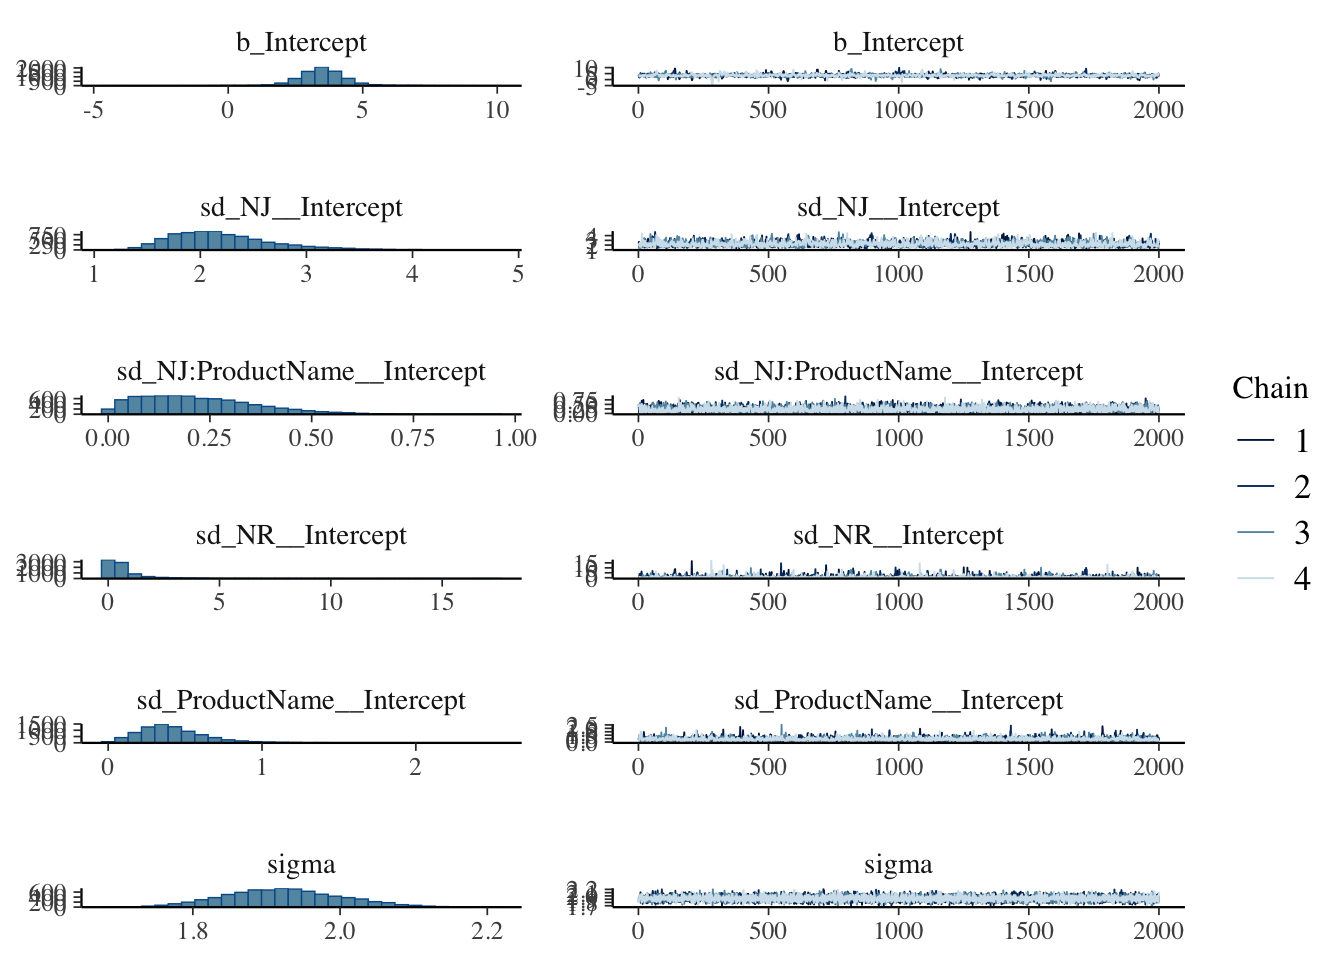
\includegraphics[keepaspectratio]{02-ANOVA_files/figure-latex/unnamed-chunk-22-1.pdf}}

We can examine the actual ``draws'' from the joint posterior using the \texttt{as\_draws\_df()} function and doing some wrangling.

\begin{Shaded}
\begin{Highlighting}[]
\NormalTok{draws }\OtherTok{\textless{}{-}} 
\NormalTok{  b\_bitter }\SpecialCharTok{\%\textgreater{}\%}
  \FunctionTok{as\_draws\_df}\NormalTok{()}

\NormalTok{draws}
\end{Highlighting}
\end{Shaded}

\begin{verbatim}
## # A draws_df: 2000 iterations, 4 chains, and 145 variables
##    b_Intercept sd_NJ__Intercept sd_NJ:ProductName__Intercept sd_NR__Intercept
## 1          3.6              2.5                        0.526           0.0733
## 2          2.3              2.7                        0.173           0.0247
## 3          3.7              1.5                        0.041           0.0055
## 4          3.3              1.6                        0.107           0.1484
## 5          3.6              2.0                        0.169           0.0308
## 6          3.3              2.1                        0.336           0.2021
## 7          3.0              1.8                        0.079           0.0586
## 8          3.2              2.0                        0.312           0.4505
## 9          3.4              2.1                        0.375           0.2390
## 10         4.4              1.5                        0.150           1.2597
##    sd_ProductName__Intercept sigma r_NJ[1331,Intercept] r_NJ[1400,Intercept]
## 1                       0.30   1.9                -0.27                -1.85
## 2                       0.59   2.0                 0.46                -0.81
## 3                       0.42   1.9                -0.55                -1.53
## 4                       0.61   1.9                -0.84                -1.96
## 5                       0.33   1.9                -0.72                -2.19
## 6                       0.38   2.0                -0.22                -2.09
## 7                       0.41   1.8                 0.20                -2.08
## 8                       0.27   2.1                -0.45                -1.58
## 9                       0.42   1.8                -0.85                -2.63
## 10                      0.82   2.0                -0.37                -2.58
## # ... with 7990 more draws, and 137 more variables
## # ... hidden reserved variables {'.chain', '.iteration', '.draw'}
\end{verbatim}

You'll note that there are a \emph{lot} of variables. We are estimating (as I understand it) deflections from the grand mean for all of the levels of all of our main effects. We can summarize these using the \texttt{posterior\_summary()} function:

\begin{Shaded}
\begin{Highlighting}[]
\FunctionTok{posterior\_summary}\NormalTok{(b\_bitter) }\SpecialCharTok{\%\textgreater{}\%}
  \FunctionTok{as\_tibble}\NormalTok{(}\AttributeTok{rownames =} \StringTok{"parameter"}\NormalTok{) }\SpecialCharTok{\%\textgreater{}\%}
  \FunctionTok{mutate}\NormalTok{(}\FunctionTok{across}\NormalTok{(}\FunctionTok{where}\NormalTok{(is.numeric), }\SpecialCharTok{\textasciitilde{}}\FunctionTok{round}\NormalTok{(., }\DecValTok{2}\NormalTok{)))}
\end{Highlighting}
\end{Shaded}

\begin{verbatim}
## # A tibble: 145 x 5
##    parameter                    Estimate Est.Error  Q2.5 Q97.5
##    <chr>                           <dbl>     <dbl> <dbl> <dbl>
##  1 b_Intercept                      3.5       0.95  1.79  5.45
##  2 sd_NJ__Intercept                 2.21      0.5   1.49  3.42
##  3 sd_NJ:ProductName__Intercept     0.22      0.14  0.02  0.55
##  4 sd_NR__Intercept                 0.74      1.15  0.03  4.04
##  5 sd_ProductName__Intercept        0.42      0.23  0.07  0.97
##  6 sigma                            1.92      0.08  1.78  2.09
##  7 r_NJ[1331,Intercept]            -0.44      0.72 -1.85  1.03
##  8 r_NJ[1400,Intercept]            -1.78      0.73 -3.22 -0.32
##  9 r_NJ[1401,Intercept]             2.34      0.72  0.96  3.8 
## 10 r_NJ[1402,Intercept]             2.31      0.72  0.92  3.74
## # i 135 more rows
\end{verbatim}

For a sanity check, notice that the estimate for our grand mean (\texttt{b\_Intercept}) is the observed value.

\begin{Shaded}
\begin{Highlighting}[]
\NormalTok{mean\_y}
\end{Highlighting}
\end{Shaded}

\begin{verbatim}
## [1] 3.494643
\end{verbatim}

\begin{Shaded}
\begin{Highlighting}[]
\NormalTok{nd }\OtherTok{\textless{}{-}} 
\NormalTok{  bayes\_data }\SpecialCharTok{\%\textgreater{}\%}
  \FunctionTok{distinct}\NormalTok{(ProductName)}

\CommentTok{\# we use \textasciigrave{}re\_formula\textasciigrave{} to marginalize across the other factors}

\NormalTok{f }\OtherTok{\textless{}{-}}
  \FunctionTok{fitted}\NormalTok{(b\_bitter,}
         \AttributeTok{newdata =}\NormalTok{ nd,}
         \AttributeTok{re\_formula =} \SpecialCharTok{\textasciitilde{}}\NormalTok{ (}\DecValTok{1} \SpecialCharTok{|}\NormalTok{ ProductName),}
         \AttributeTok{summary =} \ConstantTok{FALSE}\NormalTok{) }\SpecialCharTok{\%\textgreater{}\%}
  \FunctionTok{as\_tibble}\NormalTok{() }\SpecialCharTok{\%\textgreater{}\%}
  \FunctionTok{set\_names}\NormalTok{(nd}\SpecialCharTok{$}\NormalTok{ProductName)}

\CommentTok{\# We can look at the plausible 95\% HDI for each wine\textquotesingle{}s rated bitterness.}

\NormalTok{f }\SpecialCharTok{\%\textgreater{}\%}
  \FunctionTok{pivot\_longer}\NormalTok{(}\FunctionTok{everything}\NormalTok{()) }\SpecialCharTok{\%\textgreater{}\%}
  \FunctionTok{mutate}\NormalTok{(}\AttributeTok{name =} \FunctionTok{fct}\NormalTok{(name) }\SpecialCharTok{\%\textgreater{}\%} \FunctionTok{fct\_reorder}\NormalTok{(}\AttributeTok{.x =}\NormalTok{ value, }\AttributeTok{.fun =}\NormalTok{ mean)) }\SpecialCharTok{\%\textgreater{}\%}
  \FunctionTok{ggplot}\NormalTok{(}\FunctionTok{aes}\NormalTok{(}\AttributeTok{x =}\NormalTok{ value, }\AttributeTok{y =}\NormalTok{ name)) }\SpecialCharTok{+} 
  \FunctionTok{geom\_vline}\NormalTok{(}\AttributeTok{xintercept =} \FunctionTok{fixef}\NormalTok{(b\_bitter)[, }\DecValTok{1}\NormalTok{], }\AttributeTok{size =} \DecValTok{1}\NormalTok{, }\AttributeTok{color =} \StringTok{"red"}\NormalTok{) }\SpecialCharTok{+} 
  \FunctionTok{stat\_dotsinterval}\NormalTok{(}\AttributeTok{point\_interval =}\NormalTok{ mode\_hdi, }\AttributeTok{.width =} \FloatTok{0.95}\NormalTok{, }\AttributeTok{quantiles =} \DecValTok{100}\NormalTok{) }\SpecialCharTok{+} 
  \FunctionTok{theme\_classic}\NormalTok{() }\SpecialCharTok{+} 
  \FunctionTok{labs}\NormalTok{(}\AttributeTok{caption =} \StringTok{"Red line is the model{-}implied grand mean."}\NormalTok{)}
\end{Highlighting}
\end{Shaded}

\pandocbounded{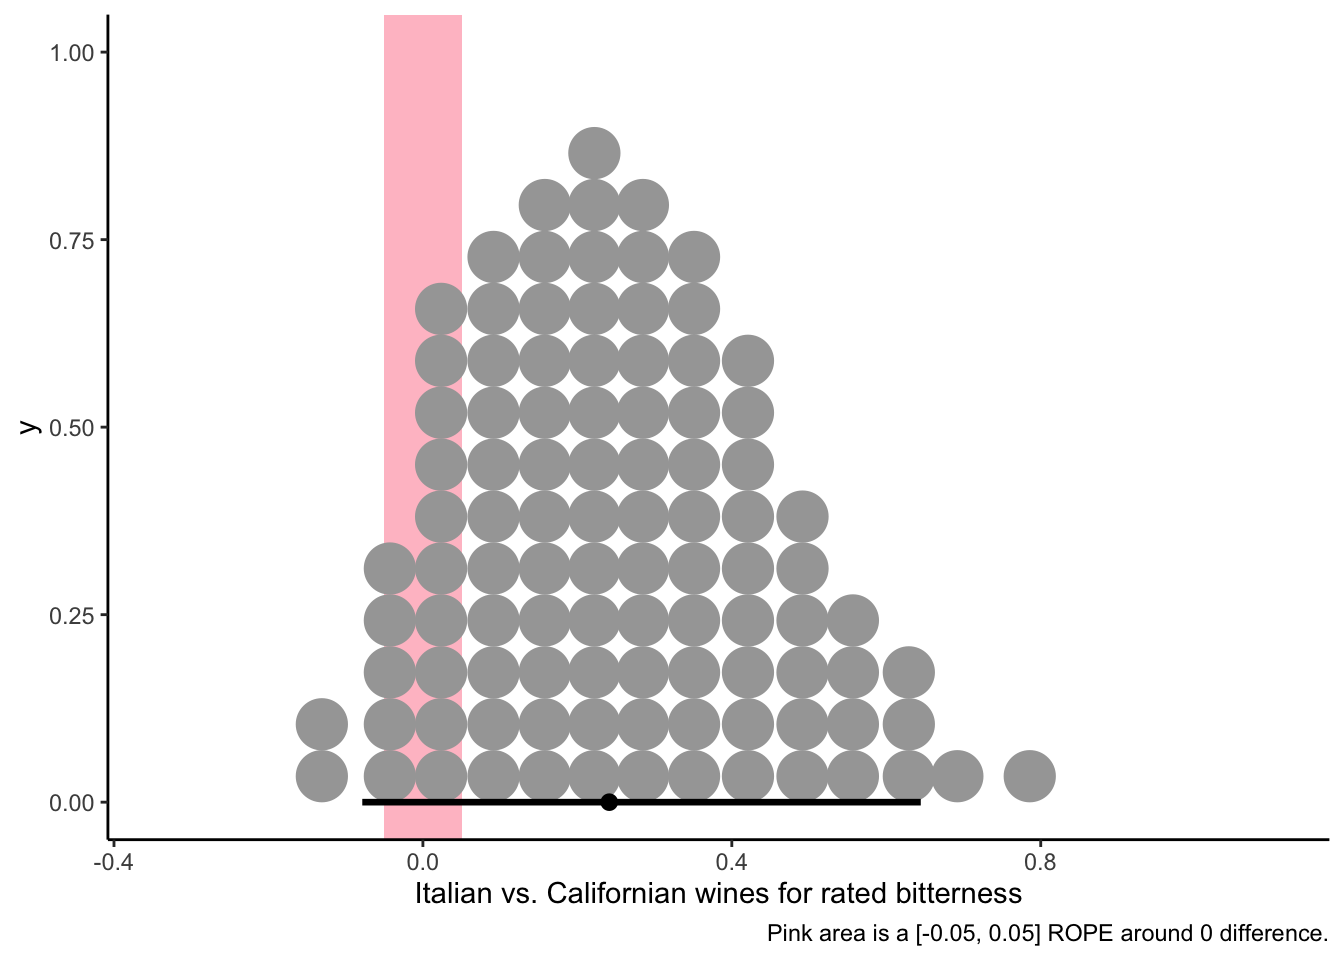
\includegraphics[keepaspectratio]{02-ANOVA_files/figure-latex/unnamed-chunk-26-1.pdf}}

It sure looks like these wines are not easy to discriminate. One advantage of Bayesian approaches is that the paradigm of investigation allows us to investigate the posterior draws to explore things like pairwise comparisons with no need to worry about ideas like ``family-wise error'' (because we are not in a hypothesis-testing framework).

\begin{Shaded}
\begin{Highlighting}[]
\CommentTok{\# Let\textquotesingle{}s see if the Italian Syrah is plausibly more bitter than the Californian Merlot:}

\NormalTok{f }\SpecialCharTok{\%\textgreater{}\%}
  \FunctionTok{transmute}\NormalTok{(}\AttributeTok{diff =}\NormalTok{ I\_SYRAH }\SpecialCharTok{{-}}\NormalTok{ C\_MERLOT) }\SpecialCharTok{\%\textgreater{}\%}
  \FunctionTok{ggplot}\NormalTok{(}\FunctionTok{aes}\NormalTok{(}\AttributeTok{x =}\NormalTok{ diff)) }\SpecialCharTok{+} 
  \FunctionTok{geom\_rect}\NormalTok{(}\FunctionTok{aes}\NormalTok{(}\AttributeTok{xmin =} \SpecialCharTok{{-}}\FloatTok{0.05}\NormalTok{, }\AttributeTok{xmax =} \FloatTok{0.05}\NormalTok{,}
                \AttributeTok{ymin =} \SpecialCharTok{{-}}\ConstantTok{Inf}\NormalTok{, }\AttributeTok{ymax =} \ConstantTok{Inf}\NormalTok{), }
            \AttributeTok{size =} \DecValTok{1}\NormalTok{, }\AttributeTok{fill =} \StringTok{"pink"}\NormalTok{, }\AttributeTok{alpha =} \DecValTok{1}\SpecialCharTok{/}\DecValTok{3}\NormalTok{) }\SpecialCharTok{+} 
  \FunctionTok{stat\_dotsinterval}\NormalTok{(}\AttributeTok{point\_interval =}\NormalTok{ mode\_hdi, }\AttributeTok{.width =} \FloatTok{0.95}\NormalTok{, }\AttributeTok{quantiles =} \DecValTok{100}\NormalTok{) }\SpecialCharTok{+} 
  \FunctionTok{theme\_classic}\NormalTok{() }\SpecialCharTok{+}
  \FunctionTok{labs}\NormalTok{(}\AttributeTok{x =} \StringTok{"Italian Syrah vs. Californian Merlot in rated bitterness"}\NormalTok{,}
       \AttributeTok{caption =} \StringTok{"Pink area is a [{-}0.05, 0.05] ROPE around 0 difference."}\NormalTok{)}
\end{Highlighting}
\end{Shaded}

\pandocbounded{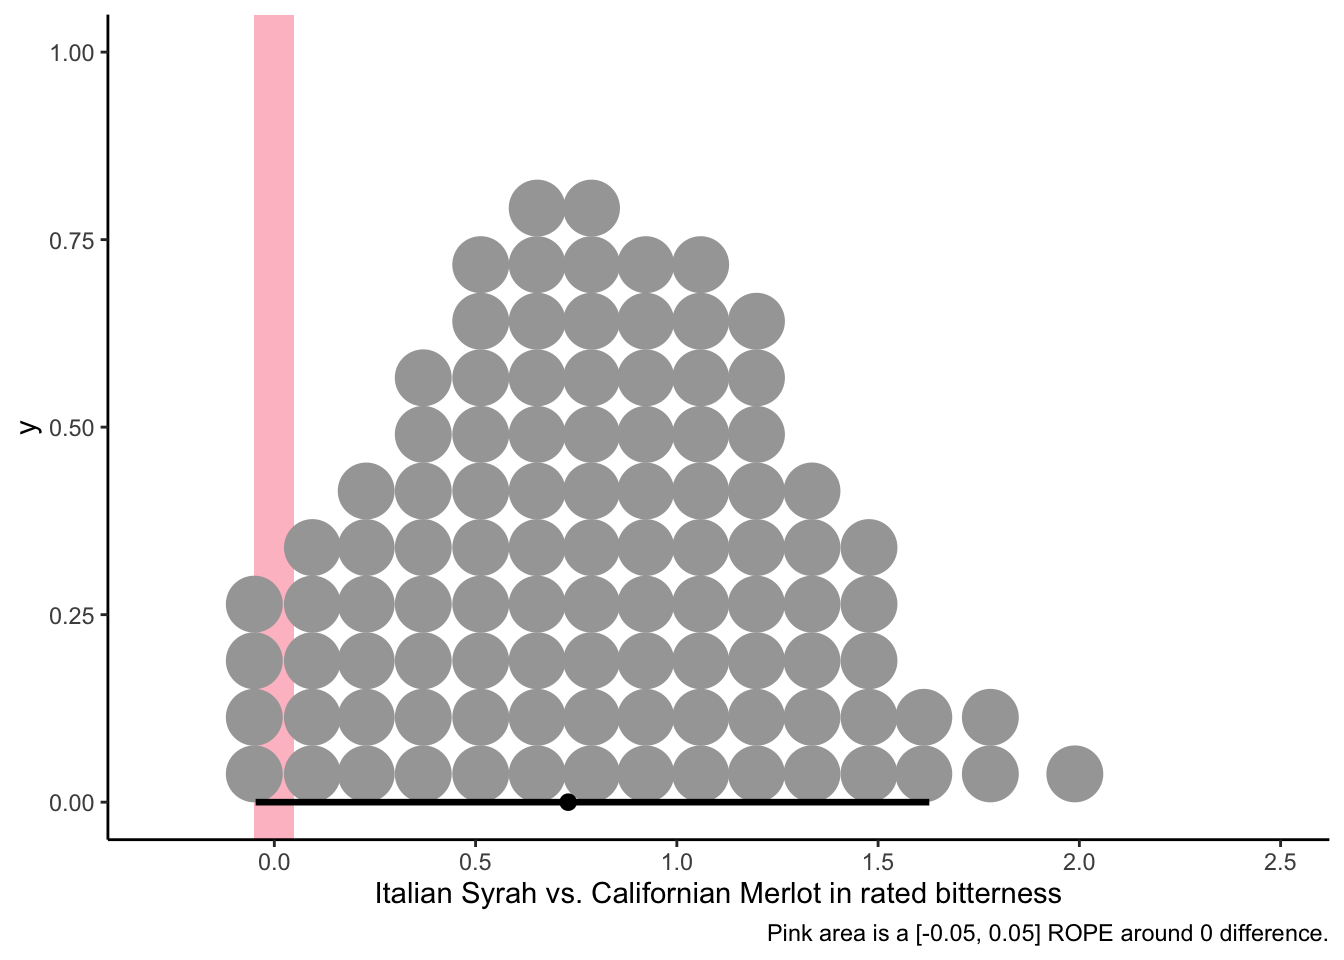
\includegraphics[keepaspectratio]{02-ANOVA_files/figure-latex/unnamed-chunk-27-1.pdf}}

It looks like the posterior differences between the most-bitter and least-bitter wines don't exclude a small ``region of plausible equivalence'' around 0 from the 95\% area of highest posterior density, so even though there is a modal difference of around 0.75 points in bitterness between these wines, we can't entirely dismiss the possibility that there is no difference in bitterness. That being said, there is at least as much posterior probability density around 1.5 points of bitterness difference, so it seems unreasonable to me to claim that these wines are exactly the same in their level of bitterness--it just probably isn't that large a difference!

We also have the freedom to explore any contrasts that might be of interest. For example, we might be interested (for either exploratory data analysis based on the HDIs above or because of \emph{a priori} theory) in knowing whether Italian wines are on average more bitter than California wines. We can do so simply:

\begin{Shaded}
\begin{Highlighting}[]
\NormalTok{f }\SpecialCharTok{\%\textgreater{}\%}
  \FunctionTok{transmute}\NormalTok{(}\AttributeTok{diff =}\NormalTok{ (I\_SYRAH }\SpecialCharTok{+}\NormalTok{ I\_MERLOT }\SpecialCharTok{+}\NormalTok{ I\_PRIMITIVO }\SpecialCharTok{+}\NormalTok{ I\_REFOSCO) }\SpecialCharTok{/} \DecValTok{4} \SpecialCharTok{{-}} 
\NormalTok{              (C\_MERLOT }\SpecialCharTok{+}\NormalTok{ C\_SYRAH }\SpecialCharTok{+}\NormalTok{ C\_ZINFANDEL }\SpecialCharTok{+}\NormalTok{ C\_REFOSCO) }\SpecialCharTok{/} \DecValTok{4}\NormalTok{) }\SpecialCharTok{\%\textgreater{}\%}
  \FunctionTok{ggplot}\NormalTok{(}\FunctionTok{aes}\NormalTok{(}\AttributeTok{x =}\NormalTok{ diff)) }\SpecialCharTok{+} 
  \FunctionTok{geom\_rect}\NormalTok{(}\FunctionTok{aes}\NormalTok{(}\AttributeTok{xmin =} \SpecialCharTok{{-}}\FloatTok{0.05}\NormalTok{, }\AttributeTok{xmax =} \FloatTok{0.05}\NormalTok{,}
                \AttributeTok{ymin =} \SpecialCharTok{{-}}\ConstantTok{Inf}\NormalTok{, }\AttributeTok{ymax =} \ConstantTok{Inf}\NormalTok{), }
            \AttributeTok{size =} \DecValTok{1}\NormalTok{, }\AttributeTok{fill =} \StringTok{"pink"}\NormalTok{, }\AttributeTok{alpha =} \DecValTok{1}\SpecialCharTok{/}\DecValTok{3}\NormalTok{) }\SpecialCharTok{+} 
  \FunctionTok{stat\_dotsinterval}\NormalTok{(}\AttributeTok{point\_interval =}\NormalTok{ mode\_hdi, }\AttributeTok{.width =} \FloatTok{0.95}\NormalTok{, }\AttributeTok{quantiles =} \DecValTok{100}\NormalTok{) }\SpecialCharTok{+} 
  \FunctionTok{theme\_classic}\NormalTok{() }\SpecialCharTok{+}
  \FunctionTok{labs}\NormalTok{(}\AttributeTok{x =} \StringTok{"Italian vs. Californian wines for rated bitterness"}\NormalTok{,}
       \AttributeTok{caption =} \StringTok{"Pink area is a [{-}0.05, 0.05] ROPE around 0 difference."}\NormalTok{)}
\end{Highlighting}
\end{Shaded}

\pandocbounded{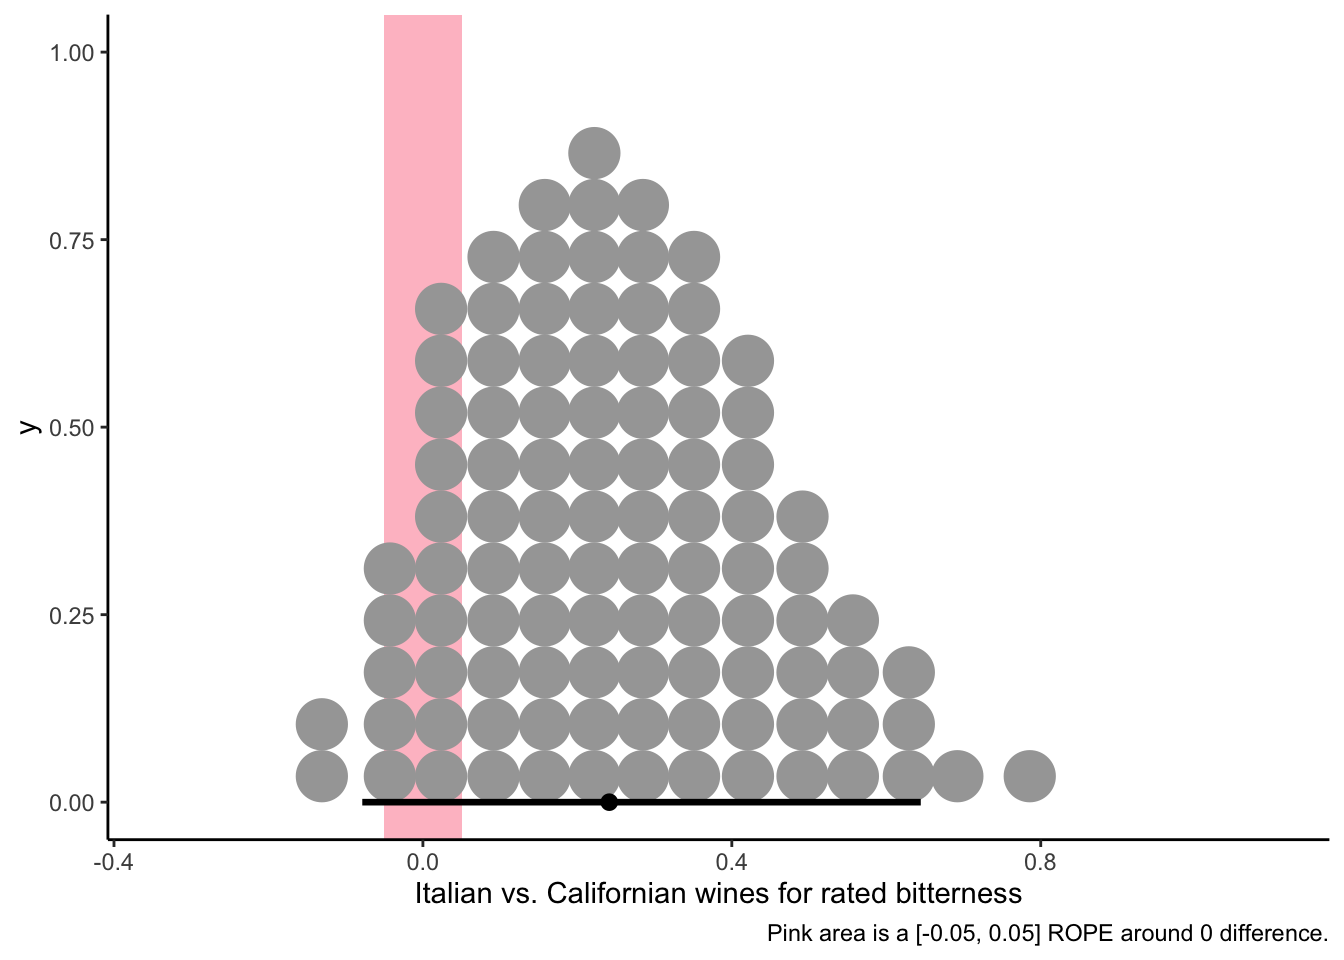
\includegraphics[keepaspectratio]{02-ANOVA_files/figure-latex/unnamed-chunk-28-1.pdf}}

Unsurprisingly, given the figures above, we see that there is some possibility of a very small amount of overall bitterness, but we'd be pretty hesitant to make broad statements when a ROPE around 0 is so clearly within the HDI for this contrast.

Finally, for my own interest, I am curious how \texttt{brms} would do using defaults in fitting the same ANOVA-like model.

\begin{Shaded}
\begin{Highlighting}[]
\NormalTok{b\_bitter\_default }\OtherTok{\textless{}{-}}
  \FunctionTok{brm}\NormalTok{(}\AttributeTok{data =}\NormalTok{ bayes\_data,}
      \AttributeTok{family =}\NormalTok{ gaussian,}
      \AttributeTok{formula =}\NormalTok{ rating }\SpecialCharTok{\textasciitilde{}} \DecValTok{1} \SpecialCharTok{+}\NormalTok{ (}\DecValTok{1} \SpecialCharTok{|}\NormalTok{ NJ) }\SpecialCharTok{+}\NormalTok{ (}\DecValTok{1} \SpecialCharTok{|}\NormalTok{ NR) }\SpecialCharTok{+}\NormalTok{ (}\DecValTok{1} \SpecialCharTok{|}\NormalTok{ ProductName) }\SpecialCharTok{+}\NormalTok{ (}\DecValTok{1} \SpecialCharTok{|}\NormalTok{ NJ}\SpecialCharTok{:}\NormalTok{ProductName),}
      \AttributeTok{seed =} \DecValTok{2}\NormalTok{, }\AttributeTok{chains =} \DecValTok{4}\NormalTok{, }\AttributeTok{cores =} \DecValTok{4}\NormalTok{, }\AttributeTok{control =} \FunctionTok{list}\NormalTok{(}\AttributeTok{adapt\_delta =} \FloatTok{0.999}\NormalTok{, }\AttributeTok{max\_treedepth =} \DecValTok{13}\NormalTok{),}
      \AttributeTok{file =} \FunctionTok{here}\NormalTok{(}\StringTok{"fits/fit\_02\_bitter\_default"}\NormalTok{))}
\end{Highlighting}
\end{Shaded}

Interestingly, this model seemed to take much less time to fit and didn't have the issues with transitions. Let's look at the chains and the parameter estimates.

\begin{Shaded}
\begin{Highlighting}[]
\NormalTok{b\_bitter\_default}
\end{Highlighting}
\end{Shaded}

\begin{verbatim}
##  Family: gaussian 
##   Links: mu = identity; sigma = identity 
## Formula: rating ~ 1 + (1 | NJ) + (1 | NR) + (1 | ProductName) + (1 | NJ:ProductName) 
##    Data: bayes_data (Number of observations: 336) 
##   Draws: 4 chains, each with iter = 2000; warmup = 1000; thin = 1;
##          total post-warmup draws = 4000
## 
## Multilevel Hyperparameters:
## ~NJ (Number of levels: 14) 
##               Estimate Est.Error l-95% CI u-95% CI Rhat Bulk_ESS Tail_ESS
## sd(Intercept)     2.16      0.48     1.45     3.31 1.01      880     1568
## 
## ~NJ:ProductName (Number of levels: 112) 
##               Estimate Est.Error l-95% CI u-95% CI Rhat Bulk_ESS Tail_ESS
## sd(Intercept)     0.19      0.14     0.01     0.52 1.00     1335     1765
## 
## ~NR (Number of levels: 3) 
##               Estimate Est.Error l-95% CI u-95% CI Rhat Bulk_ESS Tail_ESS
## sd(Intercept)     0.47      0.68     0.01     2.31 1.00     1116     1994
## 
## ~ProductName (Number of levels: 8) 
##               Estimate Est.Error l-95% CI u-95% CI Rhat Bulk_ESS Tail_ESS
## sd(Intercept)     0.39      0.22     0.05     0.92 1.00     1321     1441
## 
## Regression Coefficients:
##           Estimate Est.Error l-95% CI u-95% CI Rhat Bulk_ESS Tail_ESS
## Intercept     3.45      0.68     2.07     4.74 1.01      914     1456
## 
## Further Distributional Parameters:
##       Estimate Est.Error l-95% CI u-95% CI Rhat Bulk_ESS Tail_ESS
## sigma     1.93      0.08     1.78     2.08 1.00     5824     3043
## 
## Draws were sampled using sampling(NUTS). For each parameter, Bulk_ESS
## and Tail_ESS are effective sample size measures, and Rhat is the potential
## scale reduction factor on split chains (at convergence, Rhat = 1).
\end{verbatim}

\begin{Shaded}
\begin{Highlighting}[]
\FunctionTok{plot}\NormalTok{(b\_bitter\_default, }\AttributeTok{N =} \DecValTok{6}\NormalTok{, }\AttributeTok{width =} \FunctionTok{c}\NormalTok{(}\DecValTok{2}\NormalTok{, }\DecValTok{3}\NormalTok{))}
\end{Highlighting}
\end{Shaded}

\begin{verbatim}
## Warning: Argument 'N' is deprecated. Please use argument 'nvariables' instead.
\end{verbatim}

\pandocbounded{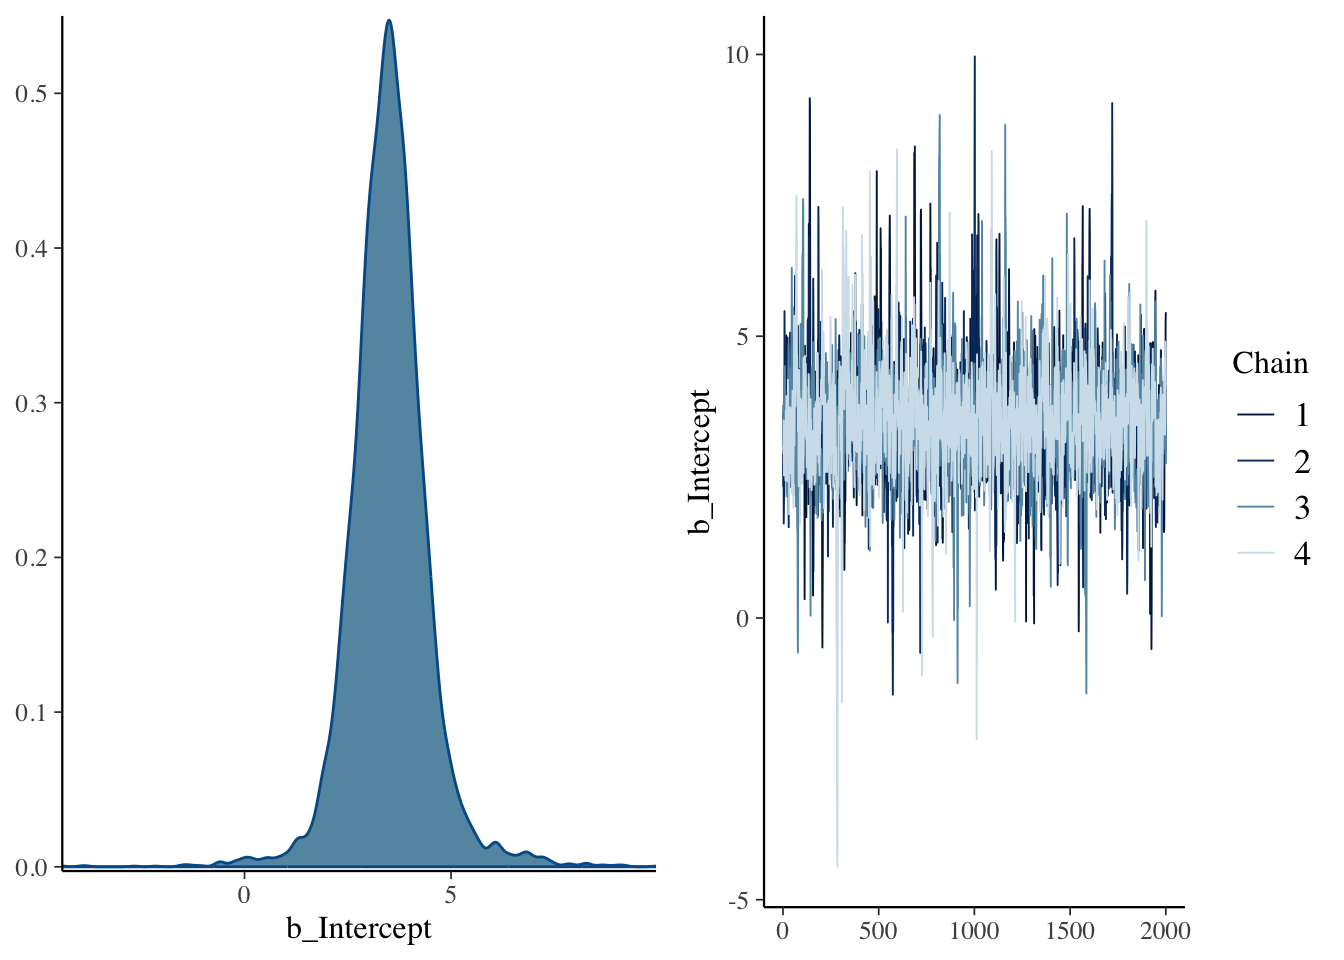
\includegraphics[keepaspectratio]{02-ANOVA_files/figure-latex/unnamed-chunk-31-1.pdf}}

It all looks ok, but it seems like the estimates for some parameters are a bit less precise, probably because we allowed the model to use uninformed priors. We can see how that was done using the \texttt{get\_prior()} function on the formula and data, as so:

\begin{Shaded}
\begin{Highlighting}[]
\FunctionTok{get\_prior}\NormalTok{(}\AttributeTok{formula =}\NormalTok{ rating }\SpecialCharTok{\textasciitilde{}} \DecValTok{1} \SpecialCharTok{+}\NormalTok{ (}\DecValTok{1} \SpecialCharTok{|}\NormalTok{ NJ) }\SpecialCharTok{+}\NormalTok{ (}\DecValTok{1} \SpecialCharTok{|}\NormalTok{ NR) }\SpecialCharTok{+}\NormalTok{ (}\DecValTok{1} \SpecialCharTok{|}\NormalTok{ ProductName) }\SpecialCharTok{+}\NormalTok{ (}\DecValTok{1} \SpecialCharTok{|}\NormalTok{ NJ}\SpecialCharTok{:}\NormalTok{ProductName),}
          \AttributeTok{data =}\NormalTok{ bayes\_data)}
\end{Highlighting}
\end{Shaded}

\begin{verbatim}
##                 prior     class      coef          group resp dpar nlpar lb ub
##  student_t(3, 3, 3.3) Intercept                                               
##  student_t(3, 0, 3.3)        sd                                           0   
##  student_t(3, 0, 3.3)        sd                       NJ                  0   
##  student_t(3, 0, 3.3)        sd Intercept             NJ                  0   
##  student_t(3, 0, 3.3)        sd           NJ:ProductName                  0   
##  student_t(3, 0, 3.3)        sd Intercept NJ:ProductName                  0   
##  student_t(3, 0, 3.3)        sd                       NR                  0   
##  student_t(3, 0, 3.3)        sd Intercept             NR                  0   
##  student_t(3, 0, 3.3)        sd              ProductName                  0   
##  student_t(3, 0, 3.3)        sd Intercept    ProductName                  0   
##  student_t(3, 0, 3.3)     sigma                                           0   
##        source
##       default
##       default
##  (vectorized)
##  (vectorized)
##  (vectorized)
##  (vectorized)
##  (vectorized)
##  (vectorized)
##  (vectorized)
##  (vectorized)
##       default
\end{verbatim}

It looks like, by default, \texttt{brm()} uses very broad Student's \(t\) priors for all the parameters; I'm no expert but I think this is what are called ``uninformed priors'' and so will be almost entirely influenced by the data. For example, if we compare our original fit following Kurz's example where we use a normal distribution with \texttt{mean} and \texttt{sd} influenced by our data, we see a distinct difference in parameter estimates for the intercept:

\begin{Shaded}
\begin{Highlighting}[]
\CommentTok{\# The original model with specified priors}
\FunctionTok{plot}\NormalTok{(b\_bitter, }\AttributeTok{variable =} \StringTok{"b\_Intercept"}\NormalTok{)}
\end{Highlighting}
\end{Shaded}

\pandocbounded{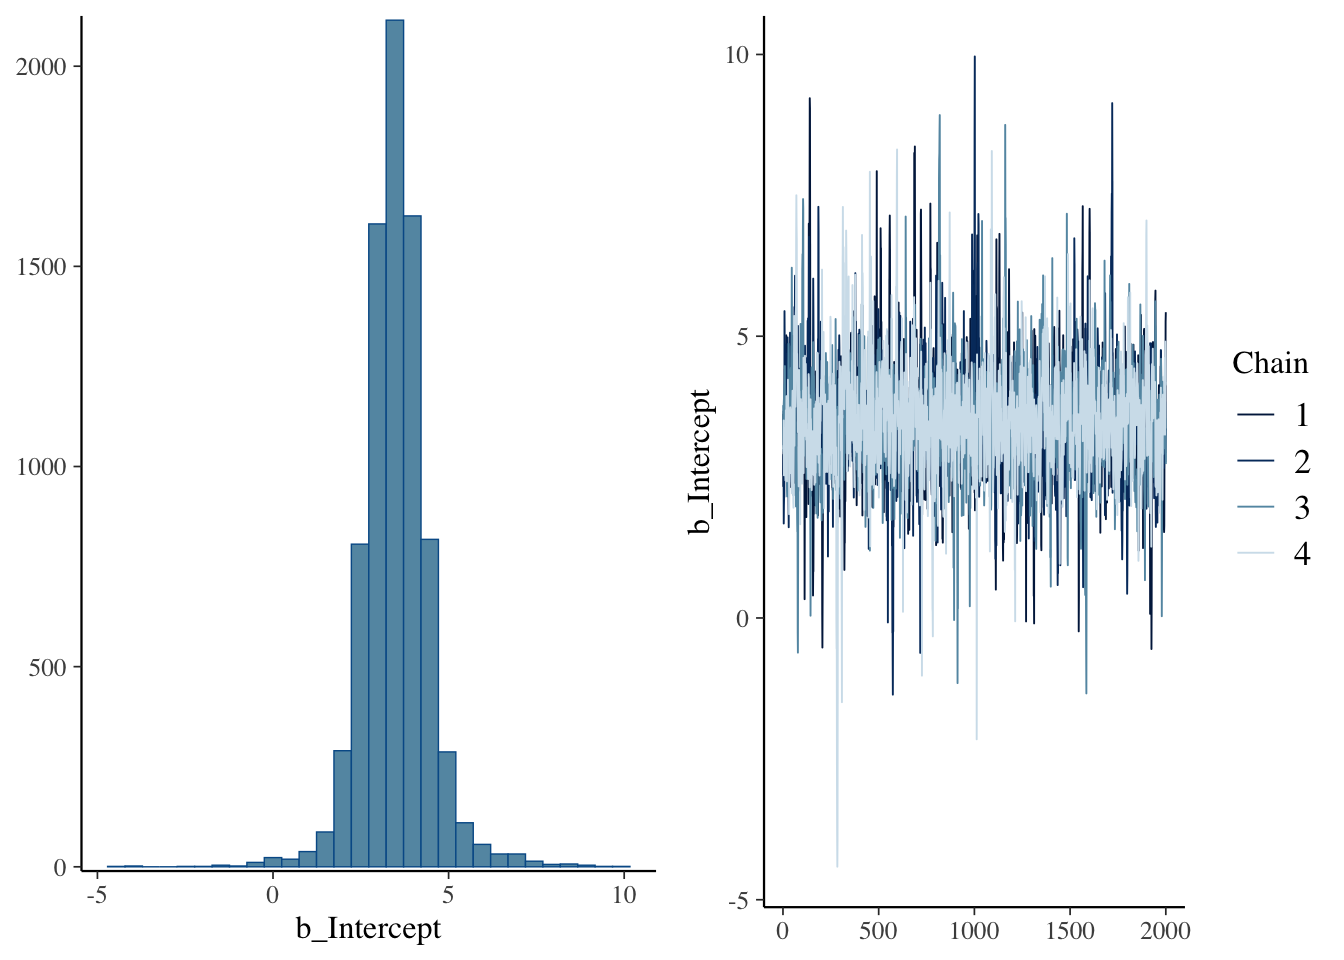
\includegraphics[keepaspectratio]{02-ANOVA_files/figure-latex/unnamed-chunk-33-1.pdf}}

\begin{Shaded}
\begin{Highlighting}[]
\CommentTok{\# The model with default priors}
\FunctionTok{plot}\NormalTok{(b\_bitter\_default, }\AttributeTok{variable =} \StringTok{"b\_Intercept"}\NormalTok{)}
\end{Highlighting}
\end{Shaded}

\pandocbounded{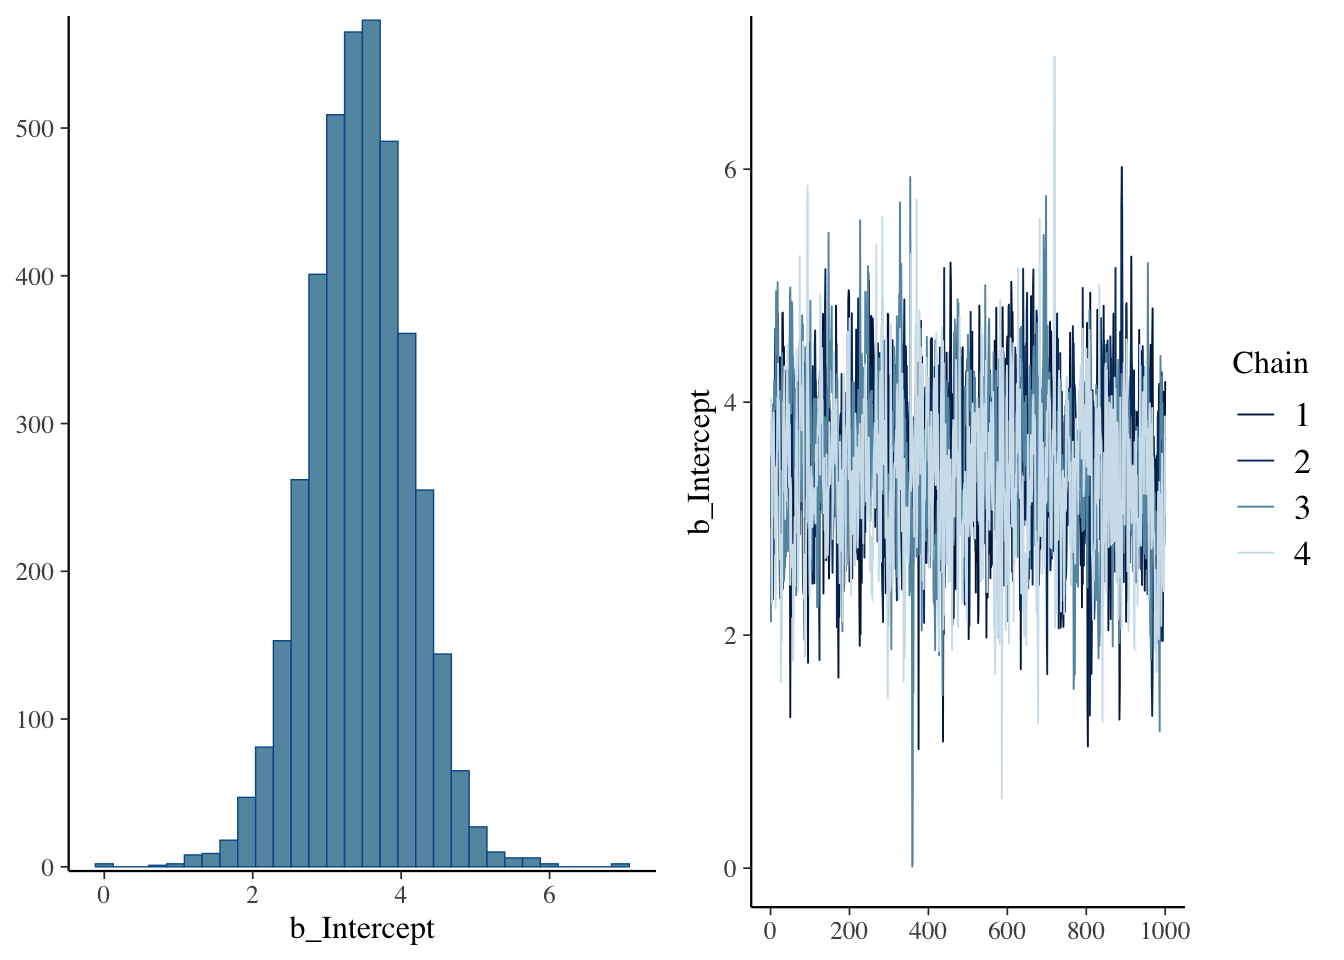
\includegraphics[keepaspectratio]{02-ANOVA_files/figure-latex/unnamed-chunk-33-2.pdf}}

So we lose some precision in exchange for speed. Let's look at how the default model predicts mean separation:

\begin{Shaded}
\begin{Highlighting}[]
\NormalTok{nd }\OtherTok{\textless{}{-}} 
\NormalTok{  bayes\_data }\SpecialCharTok{\%\textgreater{}\%}
  \FunctionTok{distinct}\NormalTok{(ProductName)}

\CommentTok{\# we use \textasciigrave{}re\_formula\textasciigrave{} to marginalize across the other factors}

\NormalTok{f }\OtherTok{\textless{}{-}}
  \FunctionTok{fitted}\NormalTok{(b\_bitter\_default,}
         \AttributeTok{newdata =}\NormalTok{ nd,}
         \AttributeTok{re\_formula =} \SpecialCharTok{\textasciitilde{}}\NormalTok{ (}\DecValTok{1} \SpecialCharTok{|}\NormalTok{ ProductName),}
         \AttributeTok{summary =} \ConstantTok{FALSE}\NormalTok{) }\SpecialCharTok{\%\textgreater{}\%}
  \FunctionTok{as\_tibble}\NormalTok{() }\SpecialCharTok{\%\textgreater{}\%}
  \FunctionTok{set\_names}\NormalTok{(nd}\SpecialCharTok{$}\NormalTok{ProductName)}

\CommentTok{\# We can look at the plausible 95\% HDI for each wine\textquotesingle{}s rated bitterness.}

\NormalTok{f }\SpecialCharTok{\%\textgreater{}\%}
  \FunctionTok{pivot\_longer}\NormalTok{(}\FunctionTok{everything}\NormalTok{()) }\SpecialCharTok{\%\textgreater{}\%}
  \FunctionTok{mutate}\NormalTok{(}\AttributeTok{name =} \FunctionTok{fct}\NormalTok{(name) }\SpecialCharTok{\%\textgreater{}\%} \FunctionTok{fct\_reorder}\NormalTok{(}\AttributeTok{.x =}\NormalTok{ value, }\AttributeTok{.fun =}\NormalTok{ mean)) }\SpecialCharTok{\%\textgreater{}\%}
  \FunctionTok{ggplot}\NormalTok{(}\FunctionTok{aes}\NormalTok{(}\AttributeTok{x =}\NormalTok{ value, }\AttributeTok{y =}\NormalTok{ name)) }\SpecialCharTok{+} 
  \FunctionTok{geom\_vline}\NormalTok{(}\AttributeTok{xintercept =} \FunctionTok{fixef}\NormalTok{(b\_bitter\_default)[, }\DecValTok{1}\NormalTok{], }\AttributeTok{size =} \DecValTok{1}\NormalTok{, }\AttributeTok{color =} \StringTok{"red"}\NormalTok{) }\SpecialCharTok{+} 
  \FunctionTok{stat\_dotsinterval}\NormalTok{(}\AttributeTok{point\_interval =}\NormalTok{ mode\_hdi, }\AttributeTok{.width =} \FloatTok{0.95}\NormalTok{, }\AttributeTok{quantiles =} \DecValTok{100}\NormalTok{) }\SpecialCharTok{+} 
  \FunctionTok{theme\_classic}\NormalTok{() }\SpecialCharTok{+} 
  \FunctionTok{labs}\NormalTok{(}\AttributeTok{caption =} \StringTok{"Red line is the model{-}implied grand mean."}\NormalTok{,}
       \AttributeTok{subtitle =} \StringTok{"The HDIs are broader with the \textasciigrave{}brms\textasciigrave{} default priors"}\NormalTok{)}
\end{Highlighting}
\end{Shaded}

\pandocbounded{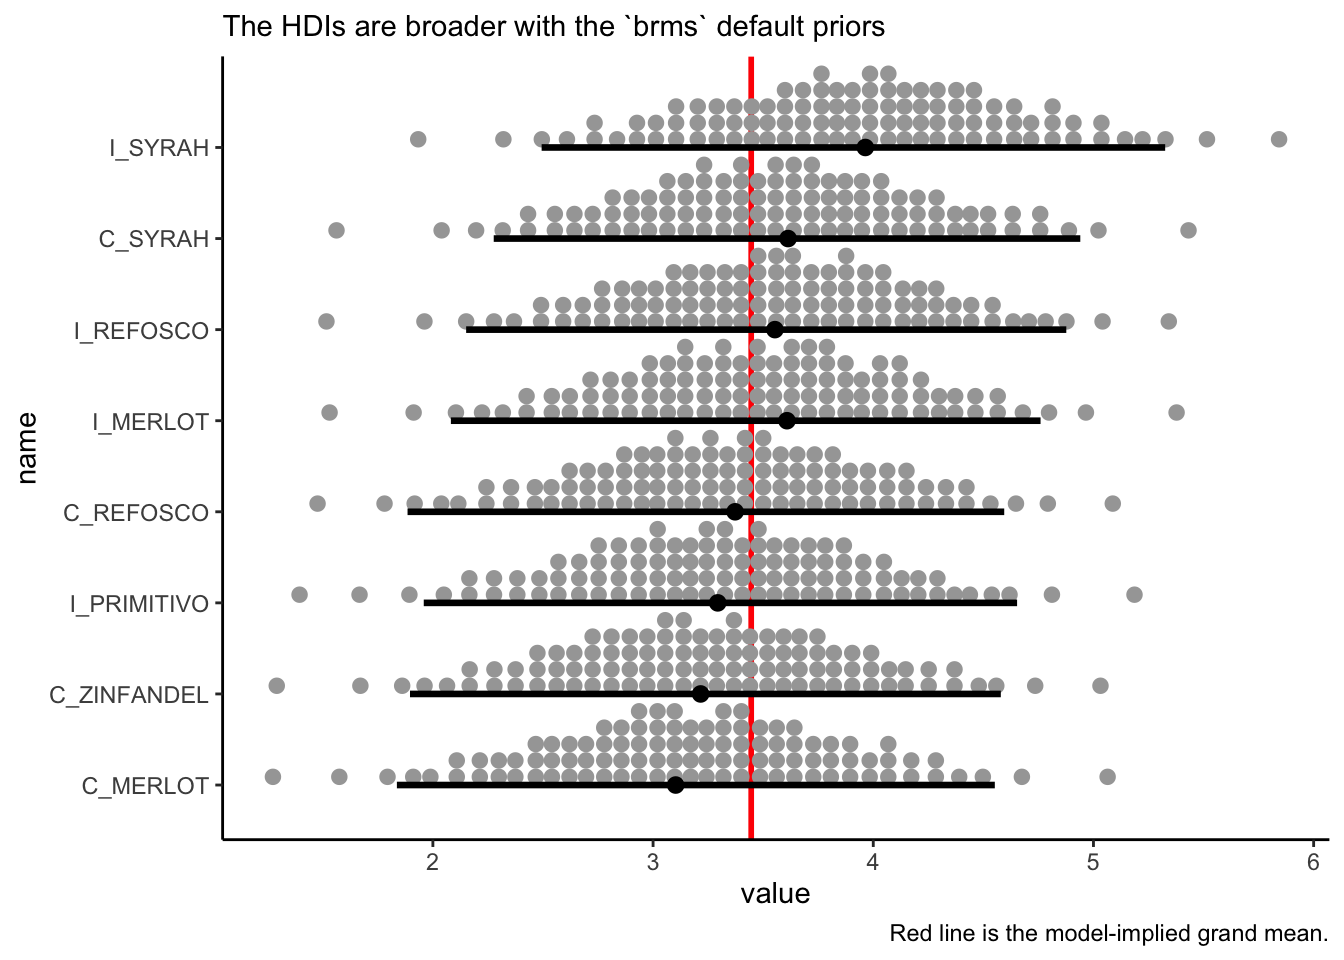
\includegraphics[keepaspectratio]{02-ANOVA_files/figure-latex/unnamed-chunk-34-1.pdf}}

And we can do the same kind of check with the individual differences:

\begin{Shaded}
\begin{Highlighting}[]
\CommentTok{\# Let\textquotesingle{}s see if the Italian Syrah is plausibly more bitter than the Californian Merlot:}

\NormalTok{f }\SpecialCharTok{\%\textgreater{}\%}
  \FunctionTok{transmute}\NormalTok{(}\AttributeTok{diff =}\NormalTok{ I\_SYRAH }\SpecialCharTok{{-}}\NormalTok{ C\_MERLOT) }\SpecialCharTok{\%\textgreater{}\%}
  \FunctionTok{ggplot}\NormalTok{(}\FunctionTok{aes}\NormalTok{(}\AttributeTok{x =}\NormalTok{ diff)) }\SpecialCharTok{+} 
  \FunctionTok{geom\_rect}\NormalTok{(}\FunctionTok{aes}\NormalTok{(}\AttributeTok{xmin =} \SpecialCharTok{{-}}\FloatTok{0.05}\NormalTok{, }\AttributeTok{xmax =} \FloatTok{0.05}\NormalTok{,}
                \AttributeTok{ymin =} \SpecialCharTok{{-}}\ConstantTok{Inf}\NormalTok{, }\AttributeTok{ymax =} \ConstantTok{Inf}\NormalTok{), }
            \AttributeTok{size =} \DecValTok{1}\NormalTok{, }\AttributeTok{fill =} \StringTok{"pink"}\NormalTok{, }\AttributeTok{alpha =} \DecValTok{1}\SpecialCharTok{/}\DecValTok{3}\NormalTok{) }\SpecialCharTok{+} 
  \FunctionTok{stat\_dotsinterval}\NormalTok{(}\AttributeTok{point\_interval =}\NormalTok{ mode\_hdi, }\AttributeTok{.width =} \FloatTok{0.95}\NormalTok{, }\AttributeTok{quantiles =} \DecValTok{100}\NormalTok{) }\SpecialCharTok{+} 
  \FunctionTok{theme\_classic}\NormalTok{() }\SpecialCharTok{+}
  \FunctionTok{labs}\NormalTok{(}\AttributeTok{x =} \StringTok{"Italian Syrah vs. Californian Merlot in rated bitterness"}\NormalTok{,}
       \AttributeTok{caption =} \StringTok{"Pink area is a [{-}0.05, 0.05] ROPE around 0 difference."}\NormalTok{,}
       \AttributeTok{subtitle =} \StringTok{"Our overall conclusions, however, would not change much using the defaults."}\NormalTok{)}
\end{Highlighting}
\end{Shaded}

\pandocbounded{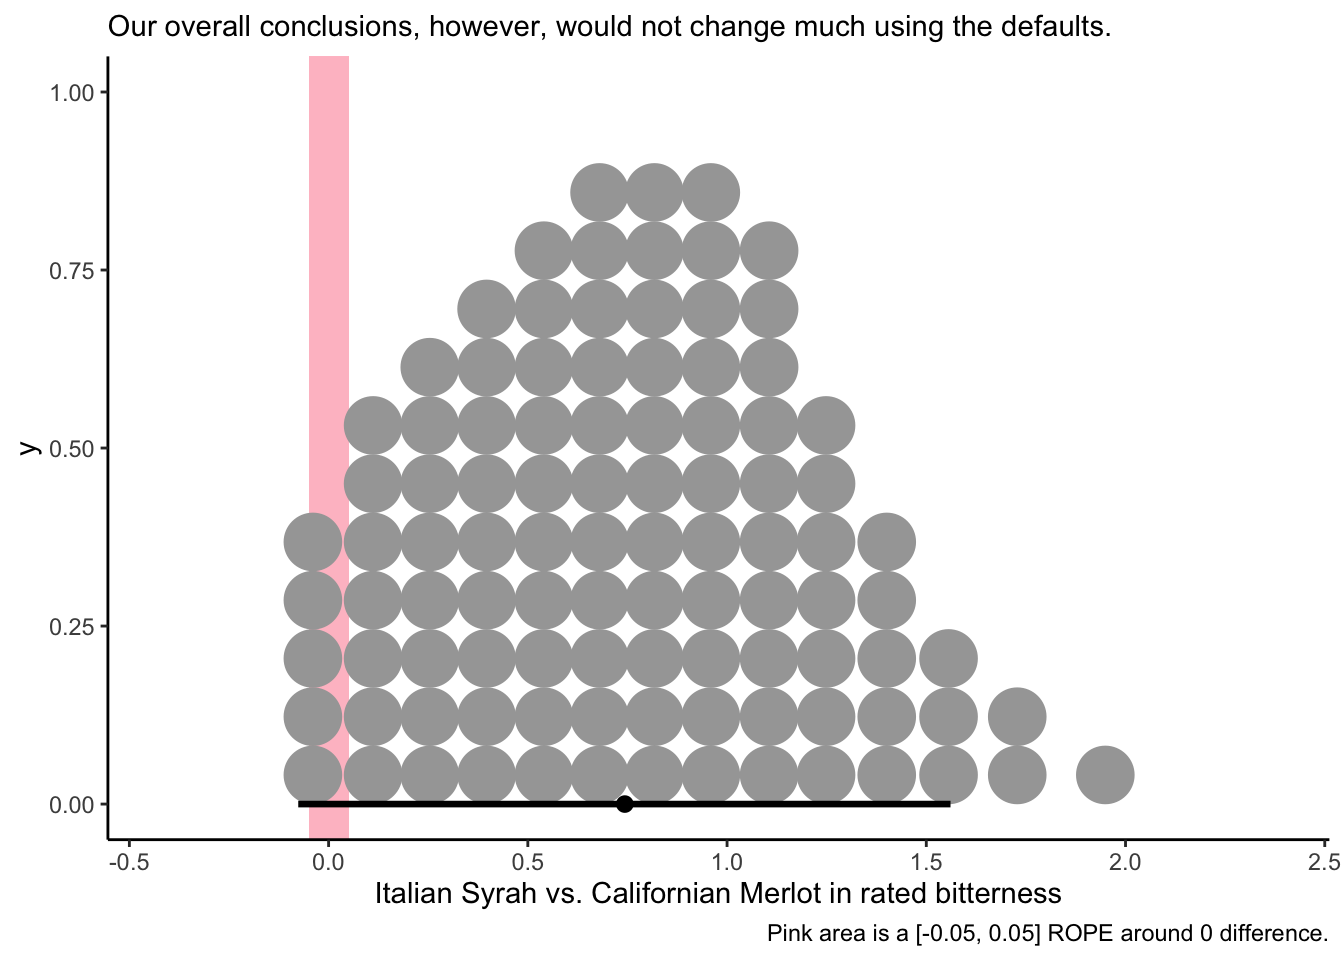
\includegraphics[keepaspectratio]{02-ANOVA_files/figure-latex/unnamed-chunk-35-1.pdf}}

So in this case, it seems like the speed of using \texttt{brms} defaults, at least for exploratory data analysis, may be worthwhile.

I might try to incorporate some more Bayesian tools as we go along, as I find them very interesting. If you want to learn more about these, I recommend the sources listed above and cited in the text here.

\section{Packages used in this chapter}\label{packages-used-in-this-chapter-1}

\begin{Shaded}
\begin{Highlighting}[]
\FunctionTok{sessionInfo}\NormalTok{()}
\end{Highlighting}
\end{Shaded}

\begin{verbatim}
## R version 4.4.1 (2024-06-14)
## Platform: x86_64-apple-darwin20
## Running under: macOS 15.2
## 
## Matrix products: default
## BLAS:   /Library/Frameworks/R.framework/Versions/4.4-x86_64/Resources/lib/libRblas.0.dylib 
## LAPACK: /Library/Frameworks/R.framework/Versions/4.4-x86_64/Resources/lib/libRlapack.dylib;  LAPACK version 3.12.0
## 
## locale:
## [1] en_US.UTF-8/en_US.UTF-8/en_US.UTF-8/C/en_US.UTF-8/en_US.UTF-8
## 
## time zone: America/New_York
## tzcode source: internal
## 
## attached base packages:
## [1] stats     graphics  grDevices datasets  utils     methods   base     
## 
## other attached packages:
##  [1] tidybayes_3.0.6 brms_2.21.0     Rcpp_1.0.13     tidytext_0.4.2 
##  [5] agricolae_1.3-7 here_1.0.1      lubridate_1.9.3 forcats_1.0.0  
##  [9] stringr_1.5.1   dplyr_1.1.4     purrr_1.0.2     readr_2.1.5    
## [13] tidyr_1.3.1     tibble_3.2.1    ggplot2_3.5.1   tidyverse_2.0.0
## 
## loaded via a namespace (and not attached):
##  [1] svUnit_1.0.6         tidyselect_1.2.1     farver_2.1.2        
##  [4] loo_2.7.0            fastmap_1.2.0        tensorA_0.36.2.1    
##  [7] janeaustenr_1.0.0    digest_0.6.37        estimability_1.5.1  
## [10] timechange_0.3.0     lifecycle_1.0.4      cluster_2.1.6       
## [13] StanHeaders_2.32.9   tokenizers_0.3.0     magrittr_2.0.3      
## [16] posterior_1.5.0      compiler_4.4.1       rlang_1.1.4         
## [19] tools_4.4.1          utf8_1.2.4           yaml_2.3.8          
## [22] knitr_1.46           labeling_0.4.3       bridgesampling_1.1-2
## [25] bit_4.0.5            pkgbuild_1.4.4       plyr_1.8.9          
## [28] abind_1.4-5          withr_3.0.0          grid_4.4.1          
## [31] stats4_4.4.1         fansi_1.0.6          AlgDesign_1.2.1     
## [34] xtable_1.8-4         colorspace_2.1-0     inline_0.3.19       
## [37] emmeans_1.10.2       scales_1.3.0         MASS_7.3-60.2       
## [40] cli_3.6.3            mvtnorm_1.2-5        rmarkdown_2.27      
## [43] crayon_1.5.2         generics_0.1.3       RcppParallel_5.1.7  
## [46] rstudioapi_0.16.0    reshape2_1.4.4       tzdb_0.4.0          
## [49] rstan_2.32.6         bayesplot_1.11.1     parallel_4.4.1      
## [52] matrixStats_1.3.0    vctrs_0.6.5          Matrix_1.7-0        
## [55] bookdown_0.39        arrayhelpers_1.1-0   hms_1.1.3           
## [58] bit64_4.0.5          ggdist_3.3.2         glue_1.7.0          
## [61] codetools_0.2-20     distributional_0.4.0 stringi_1.8.4       
## [64] gtable_0.3.5         QuickJSR_1.2.0       quadprog_1.5-8      
## [67] munsell_0.5.1        pillar_1.9.0         htmltools_0.5.8.1   
## [70] Brobdingnag_1.2-9    R6_2.5.1             rprojroot_2.0.4     
## [73] vroom_1.6.5          evaluate_0.23        lattice_0.22-6      
## [76] highr_0.10           backports_1.5.0      SnowballC_0.7.1     
## [79] broom_1.0.6          renv_1.0.9           rstantools_2.4.0    
## [82] gridExtra_2.3        coda_0.19-4.1        nlme_3.1-164        
## [85] checkmate_2.3.1      xfun_0.49            pkgconfig_2.0.3
\end{verbatim}

\chapter{Dealing with missing data}\label{dealing-with-missing-data}

In this short section, we'll look at ``single imputation'' using the Expectation Maximization approach. First, let's get our data imported and our packages set up.

\begin{Shaded}
\begin{Highlighting}[]
\FunctionTok{library}\NormalTok{(tidyverse)}
\FunctionTok{library}\NormalTok{(here)}

\NormalTok{descriptive\_data }\OtherTok{\textless{}{-}} \FunctionTok{read\_csv}\NormalTok{(}\FunctionTok{here}\NormalTok{(}\StringTok{"data/torriDAFinal.csv"}\NormalTok{))}
\NormalTok{missing\_data\_example }\OtherTok{\textless{}{-}}\FunctionTok{read\_csv}\NormalTok{(}\FunctionTok{here}\NormalTok{(}\StringTok{"data/torrimiss.csv"}\NormalTok{))}
\end{Highlighting}
\end{Shaded}

\section{Exploring missing data}\label{exploring-missing-data}

In the original \textbf{R Opus}, HGH used the \texttt{missmda} package, from Susan Josse and Francois Husson, which to my understanding uses a PCA approach to do single imputation. Reading through their documentation, they note that this is equivalent to the ``expectation maximization'' (EM) approach to single imputation. We're going to use a slightly more modern package that combines approaches from a number of different missing-data packages, called \texttt{simputation}. It gives standard syntax for a number of different formula-based methods for imputation. We're going to also use the \texttt{skimr} package to easily see where we have missing data, and the \texttt{naniar} package to visualize.

\begin{Shaded}
\begin{Highlighting}[]
\FunctionTok{library}\NormalTok{(simputation)}
\FunctionTok{library}\NormalTok{(skimr)}
\FunctionTok{library}\NormalTok{(naniar)}
\end{Highlighting}
\end{Shaded}

First off, let's take a look at our \texttt{missing\_data\_example} data set using the \texttt{skim()} method.

\begin{Shaded}
\begin{Highlighting}[]
\FunctionTok{skim}\NormalTok{(missing\_data\_example) }\SpecialCharTok{\%\textgreater{}\%} 
  \CommentTok{\# This is purely to allow the skimr::skim() to be rendered in PDF, ignore otherwise}
\NormalTok{  knitr}\SpecialCharTok{::}\FunctionTok{kable}\NormalTok{()}
\end{Highlighting}
\end{Shaded}

\begin{tabular}{l|l|r|r|r|r|r|r|r|r|r|r|r|r|r|r|l}
\hline
skim\_type & skim\_variable & n\_missing & complete\_rate & character.min & character.max & character.empty & character.n\_unique & character.whitespace & numeric.mean & numeric.sd & numeric.p0 & numeric.p25 & numeric.p50 & numeric.p75 & numeric.p100 & numeric.hist\\
\hline
character & ProductName & 0 & 1.0000000 & 7 & 11 & 0 & 8 & 0 & NA & NA & NA & NA & NA & NA & NA & NA\\
\hline
numeric & NJ & 0 & 1.0000000 & NA & NA & NA & NA & NA & 1403.3571429 & 20.8589537 & 1331 & 1402.000 & 1408.50 & 1414.000 & 1417.0 & ▁▁▁▁▇\\
\hline
numeric & NR & 0 & 1.0000000 & NA & NA & NA & NA & NA & 8.0000000 & 0.8177143 & 7 & 7.000 & 8.00 & 9.000 & 9.0 & ▇▁▇▁▇\\
\hline
numeric & Red\_berry & 11 & 0.9672619 & NA & NA & NA & NA & NA & 2.8473846 & 2.5294746 & 0 & 0.500 & 2.30 & 4.800 & 9.2 & ▇▅▂▂▁\\
\hline
numeric & Dark\_berry & 10 & 0.9702381 & NA & NA & NA & NA & NA & 3.0953988 & 2.7778038 & 0 & 0.500 & 2.30 & 5.075 & 9.9 & ▇▃▃▂▂\\
\hline
numeric & Jam & 10 & 0.9702381 & NA & NA & NA & NA & NA & 1.8773006 & 2.4022502 & 0 & 0.200 & 0.70 & 2.700 & 10.0 & ▇▂▁▁▁\\
\hline
numeric & Dried\_fruit & 10 & 0.9702381 & NA & NA & NA & NA & NA & 1.8104294 & 2.1395934 & 0 & 0.200 & 0.70 & 3.275 & 10.0 & ▇▂▂▁▁\\
\hline
numeric & Artificial\_frui & 10 & 0.9702381 & NA & NA & NA & NA & NA & 1.1996933 & 1.9710598 & 0 & 0.100 & 0.30 & 1.200 & 9.7 & ▇▁▁▁▁\\
\hline
numeric & Chocolate & 10 & 0.9702381 & NA & NA & NA & NA & NA & 1.2131902 & 1.7648302 & 0 & 0.100 & 0.40 & 1.675 & 10.0 & ▇▁▁▁▁\\
\hline
numeric & Vanilla & 11 & 0.9672619 & NA & NA & NA & NA & NA & 1.6673846 & 1.9758529 & 0 & 0.200 & 0.90 & 2.600 & 9.3 & ▇▂▁▁▁\\
\hline
numeric & Oak & 10 & 0.9702381 & NA & NA & NA & NA & NA & 2.3024540 & 1.9957632 & 0 & 0.500 & 1.70 & 3.900 & 9.0 & ▇▃▃▁▁\\
\hline
numeric & Burned & 10 & 0.9702381 & NA & NA & NA & NA & NA & 1.5070552 & 2.0622868 & 0 & 0.100 & 0.40 & 2.375 & 9.7 & ▇▂▁▁▁\\
\hline
numeric & Leather & 10 & 0.9702381 & NA & NA & NA & NA & NA & 1.4659509 & 2.0566530 & 0 & 0.100 & 0.40 & 2.400 & 9.9 & ▇▂▁▁▁\\
\hline
numeric & Earthy & 10 & 0.9702381 & NA & NA & NA & NA & NA & 1.0929448 & 1.5826888 & 0 & 0.100 & 0.40 & 1.375 & 8.0 & ▇▁▁▁▁\\
\hline
numeric & Spicy & 10 & 0.9702381 & NA & NA & NA & NA & NA & 1.2015337 & 1.6742477 & 0 & 0.100 & 0.40 & 1.800 & 8.9 & ▇▂▁▁▁\\
\hline
numeric & Pepper & 10 & 0.9702381 & NA & NA & NA & NA & NA & 1.5165644 & 2.0514989 & 0 & 0.200 & 0.50 & 2.300 & 10.0 & ▇▁▁▁▁\\
\hline
numeric & Grassy & 10 & 0.9702381 & NA & NA & NA & NA & NA & 0.9361963 & 1.4584638 & 0 & 0.100 & 0.30 & 1.100 & 9.8 & ▇▁▁▁▁\\
\hline
numeric & Medicinal & 10 & 0.9702381 & NA & NA & NA & NA & NA & 1.4276074 & 2.0269504 & 0 & 0.100 & 0.40 & 2.000 & 9.6 & ▇▁▁▁▁\\
\hline
numeric & Band-aid & 10 & 0.9702381 & NA & NA & NA & NA & NA & 1.2061350 & 2.0478189 & 0 & 0.100 & 0.30 & 1.075 & 9.8 & ▇▁▁▁▁\\
\hline
numeric & Sour & 10 & 0.9702381 & NA & NA & NA & NA & NA & 4.6199387 & 2.9908889 & 0 & 1.625 & 4.85 & 7.100 & 10.0 & ▇▅▇▆▅\\
\hline
numeric & Bitter & 10 & 0.9702381 & NA & NA & NA & NA & NA & 3.4236196 & 2.7514405 & 0 & 1.000 & 3.00 & 5.200 & 10.0 & ▇▅▃▂▂\\
\hline
numeric & Alcohol & 10 & 0.9702381 & NA & NA & NA & NA & NA & 3.6058282 & 2.4028950 & 0 & 1.200 & 4.05 & 5.200 & 9.5 & ▇▃▇▃▁\\
\hline
numeric & Astringent & 10 & 0.9702381 & NA & NA & NA & NA & NA & 4.6358896 & 2.6451989 & 0 & 2.500 & 4.70 & 6.400 & 10.0 & ▆▆▇▅▃\\
\hline
\end{tabular}

This shows us that we have (induced) missingness in all of our outcome variables (the sensory descriptors), but our predictors (\texttt{ProductName}, \texttt{NJ}, and \texttt{NR}) have no missingness, which is good. It also shows us that we need to \texttt{mutate()} the latter two of those 3 variables into factors, as right now \texttt{R} will treat them as numeric predictors.

\begin{Shaded}
\begin{Highlighting}[]
\CommentTok{\# Here we mutate the first 3 variables to all be factors}
\NormalTok{missing\_data\_example }\OtherTok{\textless{}{-}} 
\NormalTok{  missing\_data\_example }\SpecialCharTok{\%\textgreater{}\%}
  \FunctionTok{mutate\_at}\NormalTok{(}\FunctionTok{vars}\NormalTok{(}\DecValTok{1}\SpecialCharTok{:}\DecValTok{3}\NormalTok{), }\SpecialCharTok{\textasciitilde{}}\FunctionTok{as.factor}\NormalTok{(.))}

\CommentTok{\# let\textquotesingle{}s also fix this in our complete dataset before we forget}
\NormalTok{descriptive\_data }\OtherTok{\textless{}{-}}
\NormalTok{  descriptive\_data }\SpecialCharTok{\%\textgreater{}\%}
  \FunctionTok{mutate\_at}\NormalTok{(}\FunctionTok{vars}\NormalTok{(}\DecValTok{1}\SpecialCharTok{:}\DecValTok{3}\NormalTok{), }\SpecialCharTok{\textasciitilde{}}\FunctionTok{as.factor}\NormalTok{(.))}
\end{Highlighting}
\end{Shaded}

We can then get a look at the patternness of missingness using \texttt{naniar}, which has a bunch of utilities for easily visualizing missing data.

\begin{Shaded}
\begin{Highlighting}[]
\NormalTok{missing\_data\_example }\SpecialCharTok{\%\textgreater{}\%}
  \FunctionTok{vis\_miss}\NormalTok{()}
\end{Highlighting}
\end{Shaded}

\pandocbounded{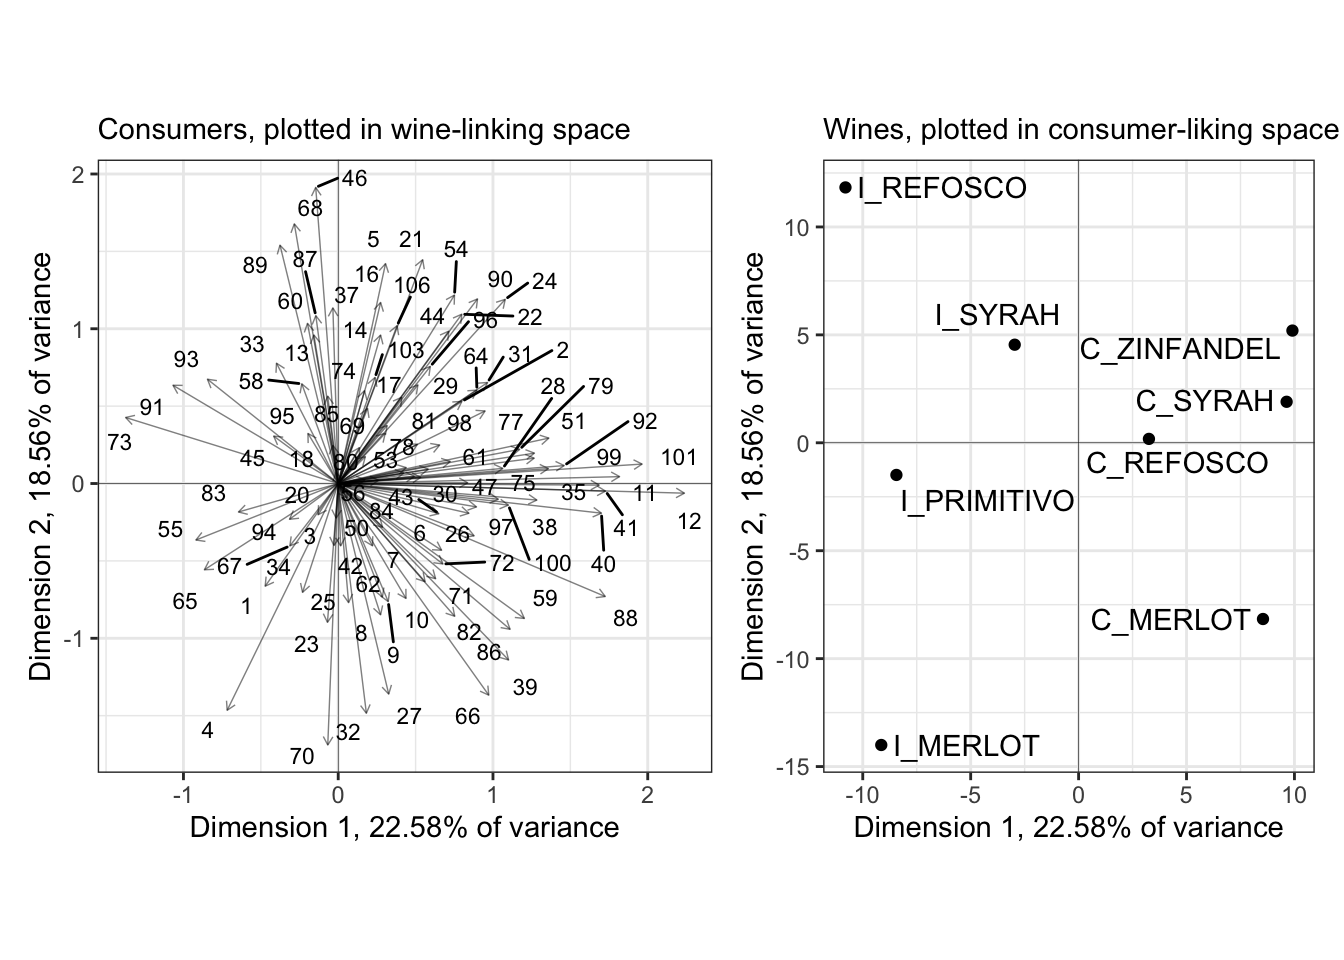
\includegraphics[keepaspectratio]{03-missing-data_files/figure-latex/unnamed-chunk-5-1.pdf}}

\begin{Shaded}
\begin{Highlighting}[]
\CommentTok{\# We see above that HGH just replaced some rows with NAs.  In this case, the}
\CommentTok{\# data is NOT missing "completely at random", as we can confirm with a}
\CommentTok{\# statistical test.}
\NormalTok{missing\_data\_example }\SpecialCharTok{\%\textgreater{}\%}
  \FunctionTok{mcar\_test}\NormalTok{()}
\end{Highlighting}
\end{Shaded}

\begin{verbatim}
## # A tibble: 1 x 4
##   statistic    df  p.value missing.patterns
##       <dbl> <dbl>    <dbl>            <int>
## 1      57.7    24 0.000133                3
\end{verbatim}

As we know that every row in our dataset is a ``case'' rather than an observation (i.e., our data is \emph{wide} rather than \emph{long}), we can use the \texttt{miss\_case\_summary()} function from \texttt{naniar} to give us a bit more info about how the missingness was introduced:

\begin{Shaded}
\begin{Highlighting}[]
\NormalTok{missing\_data\_example }\SpecialCharTok{\%\textgreater{}\%}
  \FunctionTok{miss\_case\_summary}\NormalTok{() }\SpecialCharTok{\%\textgreater{}\%}
  \FunctionTok{filter}\NormalTok{(n\_miss }\SpecialCharTok{\textgreater{}} \DecValTok{0}\NormalTok{)}
\end{Highlighting}
\end{Shaded}

\begin{verbatim}
## # A tibble: 11 x 3
##     case n_miss pct_miss
##    <int>  <int>    <dbl>
##  1     6     20    87.0 
##  2    15     20    87.0 
##  3    17     20    87.0 
##  4    18     20    87.0 
##  5    19     20    87.0 
##  6    20     20    87.0 
##  7    21     20    87.0 
##  8    22     20    87.0 
##  9    23     20    87.0 
## 10    24     20    87.0 
## 11     1      2     8.70
\end{verbatim}

The problem of missing data is a complex one, and if you have large quantities of missing data you will need to account for it in your reports. In this case, however, we're just going to accept the missingness (perhaps those subjects missed those sessions) and move on.

\section{Imputing missing data}\label{imputing-missing-data}

I am certainly no expert on missing data, but \href{https://www.jstatsoft.org/article/view/v070i01}{after doing some reading into the package HGH used in the original \textbf{R Opus}, \texttt{missMDA}}, my understanding is that this package uses a Principal Component Analysis (PCA)-based approach to imputation which is both useful for the unique problems that sensory scientists typically tackle (e.g., dealing with highly multivariate data with high uncertainty and high multicollinearity) and is competitive with current methods. Therefore, we'll use this package for imputation here, as well as showing some alternatives below.

\begin{Shaded}
\begin{Highlighting}[]
\FunctionTok{library}\NormalTok{(missMDA)}

\CommentTok{\# We can first estimate the number of components to use in our imputation.}
\CommentTok{\# NB: This may take a few minutes.}
\FunctionTok{estim\_ncpFAMD}\NormalTok{(missing\_data\_example, }\AttributeTok{verbose =} \ConstantTok{FALSE}\NormalTok{)}
\end{Highlighting}
\end{Shaded}

\begin{verbatim}
## $ncp
## [1] 5
## 
## $criterion
##        0        1        2        3        4        5 
## 2.161350 1.770345 1.577860 1.483996 1.412857 1.370000
\end{verbatim}

\begin{Shaded}
\begin{Highlighting}[]
\CommentTok{\# Then we run the imputation itself with the recommended number of components.}
\CommentTok{\# In contrast to the original R Opus, which used ncp = 2, this function}
\CommentTok{\# recommends we use ncp = 5.}

\NormalTok{missing\_data\_imputed }\OtherTok{\textless{}{-}} \FunctionTok{imputeFAMD}\NormalTok{(missing\_data\_example, }\AttributeTok{ncp =} \DecValTok{5}\NormalTok{)}

\NormalTok{missing\_data\_imputed}\SpecialCharTok{$}\NormalTok{completeObs }\SpecialCharTok{\%\textgreater{}\%}
  \FunctionTok{as\_tibble}\NormalTok{()}
\end{Highlighting}
\end{Shaded}

\begin{verbatim}
## # A tibble: 336 x 23
##    NJ    ProductName NR    Red_berry Dark_berry   Jam Dried_fruit
##    <fct> <fct>       <fct>     <dbl>      <dbl> <dbl>       <dbl>
##  1 1331  C_MERLOT    7          4.66       5.8   2.1         4.7 
##  2 1331  C_SYRAH     7          5.6        1.9   3.9         1.2 
##  3 1331  C_ZINFANDEL 7          4.9        2.6   1.4         5.9 
##  4 1331  C_REFOSCO   7          5          1.9   7.8         0.6 
##  5 1331  I__MERLOT   7          3.3        7.2   0.5         5.8 
##  6 1331  I_SYRAH     7          3.96       4.90  4.23        2.81
##  7 1331  I_PRIMITIVO 7          2.9        5.1   8.7         0.4 
##  8 1331  I_REFOSCO   7          3.2        6     4           0.7 
##  9 1400  C_MERLOT    7          0.1        0.1   0.2         2.9 
## 10 1400  C_SYRAH     7          1.6        0.7   0           6.4 
## # i 326 more rows
## # i 16 more variables: Artificial_frui <dbl>, Chocolate <dbl>, Vanilla <dbl>,
## #   Oak <dbl>, Burned <dbl>, Leather <dbl>, Earthy <dbl>, Spicy <dbl>,
## #   Pepper <dbl>, Grassy <dbl>, Medicinal <dbl>, `Band-aid` <dbl>, Sour <dbl>,
## #   Bitter <dbl>, Alcohol <dbl>, Astringent <dbl>
\end{verbatim}

We see that values have been filled in. Let's compare them to our original data visually.

\begin{Shaded}
\begin{Highlighting}[]
\NormalTok{descriptive\_data}
\end{Highlighting}
\end{Shaded}

\begin{verbatim}
## # A tibble: 336 x 23
##    NJ    ProductName NR    Red_berry Dark_berry   Jam Dried_fruit
##    <fct> <fct>       <fct>     <dbl>      <dbl> <dbl>       <dbl>
##  1 1331  C_MERLOT    7           5.1        5.8   2.1         4.7
##  2 1331  C_SYRAH     7           5.6        1.9   3.9         1.2
##  3 1331  C_ZINFANDEL 7           4.9        2.6   1.4         5.9
##  4 1331  C_REFOSCO   7           5          1.9   7.8         0.6
##  5 1331  I_MERLOT    7           3.3        7.2   0.5         5.8
##  6 1331  I_SYRAH     7           5.7        3.6   8.7         1.9
##  7 1331  I_PRIMITIVO 7           2.9        5.1   8.7         0.4
##  8 1331  I_REFOSCO   7           3.2        6     4           0.7
##  9 1400  C_MERLOT    7           0.1        0.1   0.2         2.9
## 10 1400  C_SYRAH     7           1.6        0.7   0           6.4
## # i 326 more rows
## # i 16 more variables: Artificial_frui <dbl>, Chocolate <dbl>, Vanilla <dbl>,
## #   Oak <dbl>, Burned <dbl>, Leather <dbl>, Earthy <dbl>, Spicy <dbl>,
## #   Pepper <dbl>, Grassy <dbl>, Medicinal <dbl>, `Band-aid` <dbl>, Sour <dbl>,
## #   Bitter <dbl>, Alcohol <dbl>, Astringent <dbl>
\end{verbatim}

In the first row, both \texttt{Red\_berry} and \texttt{Vanilla} were imputed. These get reasonably close. Let's compare the results of an ANOVA on the \texttt{Red\_berry} variable for the imputed and the original data.

\begin{Shaded}
\begin{Highlighting}[]
\CommentTok{\# Imputed data}
\FunctionTok{aov}\NormalTok{(Red\_berry }\SpecialCharTok{\textasciitilde{}}\NormalTok{ (ProductName }\SpecialCharTok{+}\NormalTok{ NJ }\SpecialCharTok{+}\NormalTok{ NR)}\SpecialCharTok{\^{}}\DecValTok{2}\NormalTok{, }
    \AttributeTok{data =}\NormalTok{ missing\_data\_imputed}\SpecialCharTok{$}\NormalTok{completeObs) }\SpecialCharTok{\%\textgreater{}\%}
  \FunctionTok{summary}\NormalTok{()}
\end{Highlighting}
\end{Shaded}

\begin{verbatim}
##                 Df Sum Sq Mean Sq F value   Pr(>F)    
## ProductName      7   84.1   12.01   3.532   0.0014 ** 
## NJ              13  597.3   45.95  13.510  < 2e-16 ***
## NR               2    2.9    1.45   0.425   0.6541    
## ProductName:NJ  91  639.6    7.03   2.067 1.78e-05 ***
## ProductName:NR  14   47.8    3.42   1.004   0.4509    
## NJ:NR           26   93.7    3.60   1.059   0.3940    
## Residuals      182  619.0    3.40                     
## ---
## Signif. codes:  0 '***' 0.001 '**' 0.01 '*' 0.05 '.' 0.1 ' ' 1
\end{verbatim}

\begin{Shaded}
\begin{Highlighting}[]
\CommentTok{\# Complete data}
\FunctionTok{aov}\NormalTok{(Red\_berry }\SpecialCharTok{\textasciitilde{}}\NormalTok{ (ProductName }\SpecialCharTok{+}\NormalTok{ NJ }\SpecialCharTok{+}\NormalTok{ NR)}\SpecialCharTok{\^{}}\DecValTok{2}\NormalTok{, }
    \AttributeTok{data =}\NormalTok{ descriptive\_data) }\SpecialCharTok{\%\textgreater{}\%}
  \FunctionTok{summary}\NormalTok{()}
\end{Highlighting}
\end{Shaded}

\begin{verbatim}
##                 Df Sum Sq Mean Sq F value   Pr(>F)    
## ProductName      7   73.2   10.45   2.914  0.00652 ** 
## NJ              13  597.9   45.99  12.821  < 2e-16 ***
## NR               2    2.9    1.43   0.398  0.67201    
## ProductName:NJ  91  659.0    7.24   2.019 3.18e-05 ***
## ProductName:NR  14   52.2    3.73   1.040  0.41539    
## NJ:NR           26   97.2    3.74   1.042  0.41565    
## Residuals      182  652.8    3.59                     
## ---
## Signif. codes:  0 '***' 0.001 '**' 0.01 '*' 0.05 '.' 0.1 ' ' 1
\end{verbatim}

You'll notice that the \emph{p}-value for the imputed data is actually lower! But this is an artifact, as we have not adjusted our degrees of freedom--we need to reduce our numerator degrees of freedom to account for the number of imputed values, as those values are based on the other, observed values. This will reverse this trend. We'd see something similar in the rest of the data set.

\section{Alternative approaches to imputation}\label{alternative-approaches-to-imputation}

While it is powerful, \texttt{missMDA} is not very fast, and may not be the best tool for imputation in all cases. In general, the \texttt{simputation} package has a really easy to use interface, which you can learn about by using \texttt{vignette("intro",\ package\ =\ "simputation")}. It offers a lot of competitive methods. For example, let's use a multiple regression model to predict missing variables in the dataset.

Something I've found with \texttt{simputation} is that it is flummoxed by non-syntactic names in \texttt{R}, such as \texttt{Band-aid} (you cannot typically use ``-'' in a name in \texttt{R}). We're going to quickly fix the names of our dataset in order to make it play nice before we proceed.

\begin{Shaded}
\begin{Highlighting}[]
\NormalTok{missing\_data\_imputed\_lm }\OtherTok{\textless{}{-}}
\NormalTok{  missing\_data\_example }\SpecialCharTok{\%\textgreater{}\%}
  \FunctionTok{rename\_all}\NormalTok{(}\SpecialCharTok{\textasciitilde{}}\FunctionTok{str\_replace\_all}\NormalTok{(., }\StringTok{"{-}"}\NormalTok{, }\StringTok{"\_"}\NormalTok{)) }\SpecialCharTok{\%\textgreater{}\%}
  \FunctionTok{impute\_lm}\NormalTok{(}\AttributeTok{formula =}\NormalTok{ . }\SpecialCharTok{\textasciitilde{}}\NormalTok{ ProductName }\SpecialCharTok{+}\NormalTok{ NR }\SpecialCharTok{+}\NormalTok{ NJ)}
\end{Highlighting}
\end{Shaded}

If we run the same checks as before on \texttt{Red\_berry}, let's see what we get:

\begin{Shaded}
\begin{Highlighting}[]
\CommentTok{\# Imputed data}
\FunctionTok{aov}\NormalTok{(Red\_berry }\SpecialCharTok{\textasciitilde{}}\NormalTok{ (ProductName }\SpecialCharTok{+}\NormalTok{ NJ }\SpecialCharTok{+}\NormalTok{ NR)}\SpecialCharTok{\^{}}\DecValTok{2}\NormalTok{, }
    \AttributeTok{data =}\NormalTok{ missing\_data\_imputed\_lm) }\SpecialCharTok{\%\textgreater{}\%}
  \FunctionTok{summary}\NormalTok{()}
\end{Highlighting}
\end{Shaded}

\begin{verbatim}
##                 Df Sum Sq Mean Sq F value   Pr(>F)    
## ProductName      7   90.1   12.87   3.798 0.000714 ***
## NJ              13  614.3   47.25  13.948  < 2e-16 ***
## NR               2    3.4    1.68   0.496 0.609491    
## ProductName:NJ  91  638.7    7.02   2.072 1.67e-05 ***
## ProductName:NR  14   48.3    3.45   1.018 0.437183    
## NJ:NR           26   89.3    3.43   1.014 0.451877    
## Residuals      182  616.6    3.39                     
## ---
## Signif. codes:  0 '***' 0.001 '**' 0.01 '*' 0.05 '.' 0.1 ' ' 1
\end{verbatim}

\begin{Shaded}
\begin{Highlighting}[]
\CommentTok{\# Complete data}
\FunctionTok{aov}\NormalTok{(Red\_berry }\SpecialCharTok{\textasciitilde{}}\NormalTok{ (ProductName }\SpecialCharTok{+}\NormalTok{ NJ }\SpecialCharTok{+}\NormalTok{ NR)}\SpecialCharTok{\^{}}\DecValTok{2}\NormalTok{, }
    \AttributeTok{data =}\NormalTok{ descriptive\_data) }\SpecialCharTok{\%\textgreater{}\%}
  \FunctionTok{summary}\NormalTok{()}
\end{Highlighting}
\end{Shaded}

\begin{verbatim}
##                 Df Sum Sq Mean Sq F value   Pr(>F)    
## ProductName      7   73.2   10.45   2.914  0.00652 ** 
## NJ              13  597.9   45.99  12.821  < 2e-16 ***
## NR               2    2.9    1.43   0.398  0.67201    
## ProductName:NJ  91  659.0    7.24   2.019 3.18e-05 ***
## ProductName:NR  14   52.2    3.73   1.040  0.41539    
## NJ:NR           26   97.2    3.74   1.042  0.41565    
## Residuals      182  652.8    3.59                     
## ---
## Signif. codes:  0 '***' 0.001 '**' 0.01 '*' 0.05 '.' 0.1 ' ' 1
\end{verbatim}

Why is our \emph{p}-value even smaller? If you think about it, we've filled in missing values \emph{using a linear model like the one we are analyzing}. Therefore, our hypothesis--that ratings for descriptors depend on the wine, the judge, and the rep--is leaking into our imputation. This is one reason it's critical to adjust our degrees of freedom for any hypothesis tests we use on these imputed data\ldots{} or to use non-parametric models for imputation (like the ones from \texttt{missMDA}) that don't encode our hypotheses in the first place.

\section{Packages used in this chapter}\label{packages-used-in-this-chapter-2}

\begin{Shaded}
\begin{Highlighting}[]
\FunctionTok{sessionInfo}\NormalTok{()}
\end{Highlighting}
\end{Shaded}

\begin{verbatim}
## R version 4.4.1 (2024-06-14)
## Platform: x86_64-apple-darwin20
## Running under: macOS 15.2
## 
## Matrix products: default
## BLAS:   /Library/Frameworks/R.framework/Versions/4.4-x86_64/Resources/lib/libRblas.0.dylib 
## LAPACK: /Library/Frameworks/R.framework/Versions/4.4-x86_64/Resources/lib/libRlapack.dylib;  LAPACK version 3.12.0
## 
## locale:
## [1] en_US.UTF-8/en_US.UTF-8/en_US.UTF-8/C/en_US.UTF-8/en_US.UTF-8
## 
## time zone: America/New_York
## tzcode source: internal
## 
## attached base packages:
## [1] stats     graphics  grDevices datasets  utils     methods   base     
## 
## other attached packages:
##  [1] missMDA_1.19      naniar_1.1.0      skimr_2.1.5       simputation_0.2.9
##  [5] here_1.0.1        lubridate_1.9.3   forcats_1.0.0     stringr_1.5.1    
##  [9] dplyr_1.1.4       purrr_1.0.2       readr_2.1.5       tidyr_1.3.1      
## [13] tibble_3.2.1      ggplot2_3.5.1     tidyverse_2.0.0  
## 
## loaded via a namespace (and not attached):
##  [1] tidyselect_1.2.1     farver_2.1.2         fastmap_1.2.0       
##  [4] digest_0.6.37        rpart_4.1.23         timechange_0.3.0    
##  [7] estimability_1.5.1   lifecycle_1.0.4      cluster_2.1.6       
## [10] multcompView_0.1-10  survival_3.6-4       magrittr_2.0.3      
## [13] compiler_4.4.1       rlang_1.1.4          tools_4.4.1         
## [16] utf8_1.2.4           yaml_2.3.8           knitr_1.46          
## [19] labeling_0.4.3       htmlwidgets_1.6.4    bit_4.0.5           
## [22] scatterplot3d_0.3-44 repr_1.1.7           norm_1.0-11.1       
## [25] withr_3.0.0          nnet_7.3-19          grid_4.4.1          
## [28] fansi_1.0.6          jomo_2.7-6           xtable_1.8-4        
## [31] colorspace_2.1-0     mice_3.17.0          emmeans_1.10.2      
## [34] scales_1.3.0         iterators_1.0.14     MASS_7.3-60.2       
## [37] flashClust_1.01-2    cli_3.6.3            mvtnorm_1.2-5       
## [40] rmarkdown_2.27       crayon_1.5.2         generics_0.1.3      
## [43] rstudioapi_0.16.0    tzdb_0.4.0           minqa_1.2.7         
## [46] splines_4.4.1        parallel_4.4.1       base64enc_0.1-3     
## [49] vctrs_0.6.5          boot_1.3-30          Matrix_1.7-0        
## [52] glmnet_4.1-8         jsonlite_1.8.8       bookdown_0.39       
## [55] hms_1.1.3            mitml_0.4-5          bit64_4.0.5         
## [58] visdat_0.6.0         ggrepel_0.9.5        FactoMineR_2.11     
## [61] foreach_1.5.2        gower_1.0.2          glue_1.7.0          
## [64] pan_1.9              nloptr_2.0.3         codetools_0.2-20    
## [67] DT_0.33              shape_1.4.6.1        stringi_1.8.4       
## [70] gtable_0.3.5         lme4_1.1-35.3        munsell_0.5.1       
## [73] pillar_1.9.0         htmltools_0.5.8.1    R6_2.5.1            
## [76] doParallel_1.0.17    rprojroot_2.0.4      vroom_1.6.5         
## [79] evaluate_0.23        lattice_0.22-6       highr_0.10          
## [82] backports_1.5.0      leaps_3.1            broom_1.0.6         
## [85] renv_1.0.9           Rcpp_1.0.13          nlme_3.1-164        
## [88] coda_0.19-4.1        xfun_0.49            pkgconfig_2.0.3
\end{verbatim}

\chapter{MANOVA (Multivariate Analysis of Variance)}\label{manova-multivariate-analysis-of-variance}

In this extremely brief section we'll apply a multivariate ANOVA (MANOVA) to our data. MANOVA analyzes changes in the mean vectors of outcome variables based on categorical factors. We'll spend slightly more time than HGH did in the original \textbf{R Opus} on these concepts, although \emph{only} slightly.

First, let's reload our packages and data:

\begin{Shaded}
\begin{Highlighting}[]
\FunctionTok{library}\NormalTok{(tidyverse)}
\FunctionTok{library}\NormalTok{(here)}

\NormalTok{descriptive\_data }\OtherTok{\textless{}{-}} \FunctionTok{read\_csv}\NormalTok{(}\FunctionTok{here}\NormalTok{(}\StringTok{"data/torriDAFinal.csv"}\NormalTok{)) }\SpecialCharTok{\%\textgreater{}\%}
  
  \CommentTok{\# Don\textquotesingle{}t forget to change the independent variables here to factors...}
  
  \FunctionTok{mutate\_at}\NormalTok{(}\AttributeTok{.vars =} \FunctionTok{vars}\NormalTok{(}\DecValTok{1}\SpecialCharTok{:}\DecValTok{3}\NormalTok{), }\SpecialCharTok{\textasciitilde{}}\FunctionTok{as.factor}\NormalTok{(.))}
\end{Highlighting}
\end{Shaded}

\section{Running MANOVA}\label{running-manova}

The syntax for MANOVA in \texttt{R} is very similar to that for ANOVA. However, as far as I know there isn't a \emph{great} way to use a tidy approach with \texttt{map()} and \texttt{nest()} to get \texttt{manova()} to work; from what I can tell, this has to do with \texttt{R}'s formula syntax: we can't easily specify the outcome variable (on the left side of the \texttt{\textasciitilde{}} in the formula) using the named elements of a typical \texttt{R} formula as we did in the ANOVA section. There, we could write a formula like \texttt{rating\ \textasciitilde{}\ ProductName} (I'm simplifying to save myself typing). \texttt{R} is able to interpret a single name in the formula syntax, but it will not parse something like \texttt{Red\_berry:Astringent\ \textasciitilde{}\ ProductName}, which would be necessary for MANOVA.

Instead, we have to supply the multivariate outcomes as a (named) matrix \emph{in the same (case or wide) order} as the categorical predictors. Since we don't really need this for anything else, we'll use nested function calls.

\begin{Shaded}
\begin{Highlighting}[]
\NormalTok{manova\_res }\OtherTok{\textless{}{-}} 
  \FunctionTok{manova}\NormalTok{(}\FunctionTok{as.matrix}\NormalTok{(descriptive\_data[, }\DecValTok{4}\SpecialCharTok{:}\DecValTok{23}\NormalTok{]) }\SpecialCharTok{\textasciitilde{}}\NormalTok{ (ProductName }\SpecialCharTok{+}\NormalTok{ NJ }\SpecialCharTok{+}\NormalTok{ NR)}\SpecialCharTok{\^{}}\DecValTok{2}\NormalTok{, }
         \AttributeTok{data =}\NormalTok{ descriptive\_data)}
\end{Highlighting}
\end{Shaded}

We can get a summary MANOVA table using the typical \texttt{summary()} function.

\begin{Shaded}
\begin{Highlighting}[]
\FunctionTok{summary}\NormalTok{(manova\_res, }\AttributeTok{test =} \StringTok{"W"}\NormalTok{)}
\end{Highlighting}
\end{Shaded}

\begin{verbatim}
##                 Df   Wilks approx F num Df den Df    Pr(>F)    
## ProductName      7 0.04243   4.7575    140 1093.6 < 2.2e-16 ***
## NJ              13 0.00001  12.5493    260 1819.7 < 2.2e-16 ***
## NR               2 0.64784   1.9756     40  326.0 0.0007056 ***
## ProductName:NJ  91 0.00000   1.7583   1820 3331.1 < 2.2e-16 ***
## ProductName:NR  14 0.22673   0.9414    280 1916.9 0.7387371    
## NJ:NR           26 0.02215   1.3926    520 2672.6 1.873e-07 ***
## Residuals      182                                             
## ---
## Signif. codes:  0 '***' 0.001 '**' 0.01 '*' 0.05 '.' 0.1 ' ' 1
\end{verbatim}

The \texttt{test\ =\ "W"} argument asks for Wilk's \(\Lambda\), which is for whatever reason the preferred test in sensory evaluation (HGH also prefers it). The default test provided by \texttt{R} is Pillai's \(V\). Only in rare edge cases will the two tests disagree, which you are unlikely to encounter.

In this particular case, we see that there are significant differences in group mean vectors for wine (\texttt{ProductName}) and judge (\texttt{NJ}), as well as an interaction effect (\texttt{ProductName:NJ}).

\section{What does MANOVA test?}\label{what-does-manova-test}

This isn't a statistics course. But I do feel that HGH didn't give much detail in the original \textbf{R Opus}, so let's take a second to think about MANOVA (and practice some wrangling while we're at it).

In typical ANOVA, we are interested in whether knowing the categorical predictor variables tells us something about expected value for an observation. In our case, we might want to know if knowing the wine identity (\texttt{C\_ZINFANDEL} for example) tells us something about the expected level of a sensory descriptor (for example, \texttt{Red\_berry}). With elaboration, this is always the question we are answering with ANOVA.

What are we measuring in MANOVA? Well, if we treat our data in the wide, case-based way, we are asking whether the categorical predictor variables tell us anything about \emph{all of the expected values, simultaneously}. This makes a lot of sense for our particular case: we might expect correlations among variables, and so rather than investigating variables one-by-one, as we did when we ran ANOVA, we want to take advantage of this \emph{correlation structure}.

\begin{Shaded}
\begin{Highlighting}[]
\NormalTok{descriptive\_data[, }\DecValTok{4}\SpecialCharTok{:}\DecValTok{23}\NormalTok{] }\SpecialCharTok{\%\textgreater{}\%}
  \FunctionTok{cor}\NormalTok{() }\SpecialCharTok{\%\textgreater{}\%} 
  \FunctionTok{heatmap}\NormalTok{(}\AttributeTok{revC =} \ConstantTok{TRUE}\NormalTok{)}
\end{Highlighting}
\end{Shaded}

\pandocbounded{\includegraphics[keepaspectratio]{04-MANOVA_files/figure-latex/unnamed-chunk-4-1.pdf}}

Without getting too outside our remit in the \textbf{R Opus}, MANOVA attemps to explain the variation of individual observations from their \emph{group mean-vectors}. A ``mean-vector'' is just the mean of all dependent variables for a particular set of classifying categorical predictors. So, for our data, the dependent variables are all the sensory variables. We (generally) are interested in the variation around the \textbf{wine} mean-vectors. We can see these easily using the split-apply-combine approach:

\begin{Shaded}
\begin{Highlighting}[]
\NormalTok{wine\_mean\_vectors }\OtherTok{\textless{}{-}} 
\NormalTok{  descriptive\_data }\SpecialCharTok{\%\textgreater{}\%}
  \FunctionTok{group\_by}\NormalTok{(ProductName) }\SpecialCharTok{\%\textgreater{}\%}
  \FunctionTok{summarize\_if}\NormalTok{(}\AttributeTok{.predicate =} \SpecialCharTok{\textasciitilde{}}\FunctionTok{is.numeric}\NormalTok{(.),}
               \AttributeTok{.funs =} \SpecialCharTok{\textasciitilde{}}\FunctionTok{mean}\NormalTok{(.))}

\NormalTok{wine\_mean\_vectors}
\end{Highlighting}
\end{Shaded}

\begin{verbatim}
## # A tibble: 8 x 21
##   ProductName Red_berry Dark_berry   Jam Dried_fruit Artificial_frui Chocolate
##   <fct>           <dbl>      <dbl> <dbl>       <dbl>           <dbl>     <dbl>
## 1 C_MERLOT         2.46       3.05 1.37         1.86           0.776     1.19 
## 2 C_REFOSCO        2.47       2.46 1.03         1.42           0.924     2.00 
## 3 C_SYRAH          2.46       2.93 1.75         1.68           0.883     1.42 
## 4 C_ZINFANDEL      3.08       3.06 1.98         2.06           0.864     0.969
## 5 I_MERLOT         2.79       2.35 0.843        1.85           0.574     0.783
## 6 I_PRIMITIVO      3.85       3.38 3.61         1.44           2.19      1.38 
## 7 I_REFOSCO        2.48       3.01 1.54         1.87           1.11      0.810
## 8 I_SYRAH          3.17       4.48 3.10         2.16           2.43      1.20 
## # i 14 more variables: Vanilla <dbl>, Oak <dbl>, Burned <dbl>, Leather <dbl>,
## #   Earthy <dbl>, Spicy <dbl>, Pepper <dbl>, Grassy <dbl>, Medicinal <dbl>,
## #   `Band-aid` <dbl>, Sour <dbl>, Bitter <dbl>, Alcohol <dbl>, Astringent <dbl>
\end{verbatim}

We want to know whether an observation from a particular wine is significantly ``closer'' to that wine's mean-vector than it is to other wine's mean-vectors. We test this using the \href{https://en.wikipedia.org/wiki/Mahalanobis_distance}{Mahalanobis Distance}, which is a generalization of the normalized distance (or \emph{z}-score) from univariate statistics. Intuitively, we ask about the (multi-dimensional) distance of an observation from a mean-vector, divided by the covariance of the observations (the multivariate equivalent of standard deviation). Without getting into mathematics, we can ask about this distance using the \texttt{mahalanobis()} function.

\begin{Shaded}
\begin{Highlighting}[]
\NormalTok{distance\_from\_grand\_mean }\OtherTok{\textless{}{-}} 
\NormalTok{  descriptive\_data[, }\SpecialCharTok{{-}}\NormalTok{(}\DecValTok{1}\SpecialCharTok{:}\DecValTok{3}\NormalTok{)] }\SpecialCharTok{\%\textgreater{}\%}
  \FunctionTok{as.matrix}\NormalTok{() }\SpecialCharTok{\%\textgreater{}\%}
  \FunctionTok{mahalanobis}\NormalTok{(}\AttributeTok{x =}\NormalTok{ ., }\AttributeTok{center =} \FunctionTok{colMeans}\NormalTok{(.), }\AttributeTok{cov =} \FunctionTok{cov}\NormalTok{(.))}

\NormalTok{descriptive\_data }\SpecialCharTok{\%\textgreater{}\%}
  \FunctionTok{select}\NormalTok{(}\SpecialCharTok{{-}}\NormalTok{NJ, }\SpecialCharTok{{-}}\NormalTok{NR) }\SpecialCharTok{\%\textgreater{}\%}
  \FunctionTok{nest}\NormalTok{(}\AttributeTok{data =} \SpecialCharTok{{-}}\NormalTok{ProductName) }\SpecialCharTok{\%\textgreater{}\%}
  \FunctionTok{mutate}\NormalTok{(}\AttributeTok{data =} \FunctionTok{map}\NormalTok{(data, }\SpecialCharTok{\textasciitilde{}}\FunctionTok{as.matrix}\NormalTok{(.x)), }
         \AttributeTok{distance\_from\_group\_mean =} \FunctionTok{map}\NormalTok{(data, }\SpecialCharTok{\textasciitilde{}}\FunctionTok{mahalanobis}\NormalTok{(}\AttributeTok{x =}\NormalTok{ .x, }\AttributeTok{center =} \FunctionTok{colMeans}\NormalTok{(.x), }\AttributeTok{cov =} \FunctionTok{cov}\NormalTok{(.x)))) }\SpecialCharTok{\%\textgreater{}\%}
  \FunctionTok{select}\NormalTok{(}\SpecialCharTok{{-}}\NormalTok{data) }\SpecialCharTok{\%\textgreater{}\%}
  \FunctionTok{unnest}\NormalTok{(distance\_from\_group\_mean) }\SpecialCharTok{\%\textgreater{}\%}
  \FunctionTok{mutate}\NormalTok{(}\AttributeTok{distance\_from\_grand\_mean =}\NormalTok{ distance\_from\_grand\_mean) }\SpecialCharTok{\%\textgreater{}\%}
  \FunctionTok{pivot\_longer}\NormalTok{(}\SpecialCharTok{{-}}\NormalTok{ProductName) }\SpecialCharTok{\%\textgreater{}\%}
  \FunctionTok{ggplot}\NormalTok{(}\FunctionTok{aes}\NormalTok{(}\AttributeTok{x =}\NormalTok{ value, }\AttributeTok{color =}\NormalTok{ ProductName, }\AttributeTok{linetype =}\NormalTok{ name)) }\SpecialCharTok{+}
  \FunctionTok{geom\_density}\NormalTok{() }\SpecialCharTok{+}
  \FunctionTok{geom\_rug}\NormalTok{() }\SpecialCharTok{+}
  \FunctionTok{theme\_bw}\NormalTok{() }\SpecialCharTok{+}
  \FunctionTok{labs}\NormalTok{(}\AttributeTok{x =} \StringTok{"Mahalanobis distance from wine (group) and grand (overall) mean"}\NormalTok{) }\SpecialCharTok{+}
  \FunctionTok{facet\_wrap}\NormalTok{(}\SpecialCharTok{\textasciitilde{}}\NormalTok{ProductName)}
\end{Highlighting}
\end{Shaded}

\pandocbounded{\includegraphics[keepaspectratio]{04-MANOVA_files/figure-latex/unnamed-chunk-6-1.pdf}}

In this plot, we're able to see how far each individual row (observation) is, in a standardized, multivariate space, from the group mean (the dashed line) and the grand mean (the solid line). We can see that our groups are not necessarily well-defined: often, the grand mean seems to do a better job of describing our samples than the group mean for the specific wine. This might be a sign of our panelists needing further training, but recall that this (simple) visualization doesn't account for variance stemming from replicate and individual judge scaling behavior, nuisance factors that we actually included in the real MANOVA we ran above. When we include these, we find that in fact group membership (the type of wine) is important for predicting the sample mean vector.

\begin{Shaded}
\begin{Highlighting}[]
\NormalTok{descriptive\_data }\SpecialCharTok{\%\textgreater{}\%}
  \FunctionTok{select}\NormalTok{(}\SpecialCharTok{{-}}\NormalTok{ProductName, }\SpecialCharTok{{-}}\NormalTok{NJ) }\SpecialCharTok{\%\textgreater{}\%}
  \FunctionTok{nest}\NormalTok{(}\AttributeTok{data =} \SpecialCharTok{{-}}\NormalTok{NR) }\SpecialCharTok{\%\textgreater{}\%}
  \FunctionTok{mutate}\NormalTok{(}\AttributeTok{data =} \FunctionTok{map}\NormalTok{(data, }\SpecialCharTok{\textasciitilde{}}\FunctionTok{as.matrix}\NormalTok{(.x)), }
         \AttributeTok{distance\_from\_group\_mean =} \FunctionTok{map}\NormalTok{(data, }\SpecialCharTok{\textasciitilde{}}\FunctionTok{mahalanobis}\NormalTok{(}\AttributeTok{x =}\NormalTok{ .x, }\AttributeTok{center =} \FunctionTok{colMeans}\NormalTok{(.x), }\AttributeTok{cov =} \FunctionTok{cov}\NormalTok{(.x)))) }\SpecialCharTok{\%\textgreater{}\%}
  \FunctionTok{select}\NormalTok{(}\SpecialCharTok{{-}}\NormalTok{data) }\SpecialCharTok{\%\textgreater{}\%}
  \FunctionTok{unnest}\NormalTok{(distance\_from\_group\_mean) }\SpecialCharTok{\%\textgreater{}\%}
  \FunctionTok{mutate}\NormalTok{(}\AttributeTok{distance\_from\_grand\_mean =}\NormalTok{ distance\_from\_grand\_mean) }\SpecialCharTok{\%\textgreater{}\%}
  \FunctionTok{pivot\_longer}\NormalTok{(}\SpecialCharTok{{-}}\NormalTok{NR) }\SpecialCharTok{\%\textgreater{}\%}
  \FunctionTok{ggplot}\NormalTok{(}\FunctionTok{aes}\NormalTok{(}\AttributeTok{x =}\NormalTok{ value, }\AttributeTok{color =}\NormalTok{ NR, }\AttributeTok{linetype =}\NormalTok{ name)) }\SpecialCharTok{+}
  \FunctionTok{geom\_density}\NormalTok{() }\SpecialCharTok{+}
  \FunctionTok{geom\_rug}\NormalTok{() }\SpecialCharTok{+}
  \FunctionTok{theme\_bw}\NormalTok{() }\SpecialCharTok{+}
  \FunctionTok{labs}\NormalTok{(}\AttributeTok{x =} \StringTok{"Mahalanobis distance from rep (group) and grand (overall) mean"}\NormalTok{) }\SpecialCharTok{+}
  \FunctionTok{facet\_wrap}\NormalTok{(}\SpecialCharTok{\textasciitilde{}}\NormalTok{NR)}
\end{Highlighting}
\end{Shaded}

\pandocbounded{\includegraphics[keepaspectratio]{04-MANOVA_files/figure-latex/unnamed-chunk-7-1.pdf}}

Here we can see that the distribution is almost identical, meaning that knowing what replication (\texttt{NR}) the observation comes from gives us almost no new information. This is good news, because we don't \emph{want} the replication to predict anything about the sensory quality of our wines!

We would display the same plot for our judges (\texttt{NJ}), but some of our judges are TOO repeatable: they have singular covariance matrices (we can tell because the determinant of their covariance matrices is 0), which indicates that the rank of their covariance matrix is less than the number of attributes. This in turn leads to a situation in which their product descriptions are lower-dimensional than the data.

\begin{Shaded}
\begin{Highlighting}[]
\NormalTok{descriptive\_data }\SpecialCharTok{\%\textgreater{}\%}
  \FunctionTok{select}\NormalTok{(}\SpecialCharTok{{-}}\NormalTok{ProductName, }\SpecialCharTok{{-}}\NormalTok{NR) }\SpecialCharTok{\%\textgreater{}\%}
  \FunctionTok{nest}\NormalTok{(}\AttributeTok{data =} \SpecialCharTok{{-}}\NormalTok{NJ) }\SpecialCharTok{\%\textgreater{}\%}
  \FunctionTok{mutate}\NormalTok{(}\AttributeTok{data =} \FunctionTok{map}\NormalTok{(data, }\SpecialCharTok{\textasciitilde{}}\FunctionTok{as.matrix}\NormalTok{(.x)),}
         \AttributeTok{covariance\_matrix =} \FunctionTok{map}\NormalTok{(data, }\SpecialCharTok{\textasciitilde{}}\FunctionTok{cov}\NormalTok{(.x)),}
         \AttributeTok{determinant =} \FunctionTok{map\_dbl}\NormalTok{(covariance\_matrix, }\SpecialCharTok{\textasciitilde{}}\FunctionTok{det}\NormalTok{(.x)))}
\end{Highlighting}
\end{Shaded}

\begin{verbatim}
## # A tibble: 14 x 4
##    NJ    data            covariance_matrix determinant
##    <fct> <list>          <list>                  <dbl>
##  1 1331  <dbl [24 x 20]> <dbl [20 x 20]>      5.21e+ 2
##  2 1400  <dbl [24 x 20]> <dbl [20 x 20]>      1.86e- 6
##  3 1401  <dbl [24 x 20]> <dbl [20 x 20]>      1.57e-10
##  4 1402  <dbl [24 x 20]> <dbl [20 x 20]>      1.56e-16
##  5 1404  <dbl [24 x 20]> <dbl [20 x 20]>      0       
##  6 1405  <dbl [24 x 20]> <dbl [20 x 20]>      5.16e- 1
##  7 1408  <dbl [24 x 20]> <dbl [20 x 20]>      2.73e-21
##  8 1409  <dbl [24 x 20]> <dbl [20 x 20]>      5.75e-13
##  9 1412  <dbl [24 x 20]> <dbl [20 x 20]>      3.09e- 3
## 10 1413  <dbl [24 x 20]> <dbl [20 x 20]>      0       
## 11 1414  <dbl [24 x 20]> <dbl [20 x 20]>      1.68e- 8
## 12 1415  <dbl [24 x 20]> <dbl [20 x 20]>      5.55e+ 5
## 13 1416  <dbl [24 x 20]> <dbl [20 x 20]>      7.86e+ 1
## 14 1417  <dbl [24 x 20]> <dbl [20 x 20]>      1.31e- 4
\end{verbatim}

Let's take a quick look at subject 1404's ratings:

\begin{Shaded}
\begin{Highlighting}[]
\NormalTok{descriptive\_data }\SpecialCharTok{\%\textgreater{}\%}
  \FunctionTok{filter}\NormalTok{(NJ }\SpecialCharTok{==} \StringTok{"1404"}\NormalTok{)}
\end{Highlighting}
\end{Shaded}

\begin{verbatim}
## # A tibble: 24 x 23
##    NJ    ProductName NR    Red_berry Dark_berry   Jam Dried_fruit
##    <fct> <fct>       <fct>     <dbl>      <dbl> <dbl>       <dbl>
##  1 1404  C_MERLOT    7           4          5.6   0           0  
##  2 1404  C_SYRAH     7           0.5        7.5   0           4.4
##  3 1404  C_ZINFANDEL 7           4.9        7.9   0.5         1.9
##  4 1404  C_REFOSCO   7           0.3        1.8   0           0  
##  5 1404  I_MERLOT    7           0.7        5.1   0           5.2
##  6 1404  I_SYRAH     7           5.2        4     4           2.9
##  7 1404  I_PRIMITIVO 7           6.4        8.8   7.6         1  
##  8 1404  I_REFOSCO   7           3.7        4.8   3.8         3.9
##  9 1404  C_MERLOT    8           3.4        8.3   3.5         4.6
## 10 1404  C_SYRAH     8           3          8.8   3           4.3
## # i 14 more rows
## # i 16 more variables: Artificial_frui <dbl>, Chocolate <dbl>, Vanilla <dbl>,
## #   Oak <dbl>, Burned <dbl>, Leather <dbl>, Earthy <dbl>, Spicy <dbl>,
## #   Pepper <dbl>, Grassy <dbl>, Medicinal <dbl>, `Band-aid` <dbl>, Sour <dbl>,
## #   Bitter <dbl>, Alcohol <dbl>, Astringent <dbl>
\end{verbatim}

Because this subject never used ``Chocolate'' or ``Band-aid'' descriptors, they end up with a rank-deficient covariance matrix:

\begin{Shaded}
\begin{Highlighting}[]
\NormalTok{descriptive\_data }\SpecialCharTok{\%\textgreater{}\%}
  \FunctionTok{filter}\NormalTok{(NJ }\SpecialCharTok{==} \StringTok{"1404"}\NormalTok{) }\SpecialCharTok{\%\textgreater{}\%}
  \FunctionTok{select}\NormalTok{(}\SpecialCharTok{{-}}\NormalTok{(}\DecValTok{1}\SpecialCharTok{:}\DecValTok{3}\NormalTok{)) }\SpecialCharTok{\%\textgreater{}\%}
  \FunctionTok{cov}\NormalTok{() }\SpecialCharTok{\%\textgreater{}\%}
  \FunctionTok{round}\NormalTok{(}\DecValTok{2}\NormalTok{)}
\end{Highlighting}
\end{Shaded}

\begin{verbatim}
##                 Red_berry Dark_berry   Jam Dried_fruit Artificial_frui
## Red_berry            5.42       3.66  5.73        0.65            1.81
## Dark_berry           3.66       6.83  4.92        2.96            0.82
## Jam                  5.73       4.92  8.92        1.95            2.48
## Dried_fruit          0.65       2.96  1.95        3.61            0.22
## Artificial_frui      1.81       0.82  2.48        0.22            1.65
## Chocolate            0.00       0.00  0.00        0.00            0.00
## Vanilla              0.38       0.91 -0.48        0.22           -0.10
## Oak                 -0.28      -0.02 -2.02       -0.56           -0.66
## Burned              -4.74      -4.98 -5.14       -3.26           -1.65
## Leather             -0.29      -0.31 -0.28       -0.08           -0.09
## Earthy              -0.15      -0.20 -0.35       -0.18           -0.05
## Spicy                0.10      -0.30 -0.58       -0.19           -0.21
## Pepper              -0.53      -0.10 -1.45       -0.33           -0.53
## Grassy               0.14       0.07  0.12       -0.06            0.05
## Medicinal           -1.20      -1.46 -0.80        1.31           -0.39
## Band-aid             0.00       0.00  0.00        0.00            0.00
## Sour                -0.33       0.15 -0.72        0.81           -0.34
## Bitter              -0.10      -0.13 -0.38       -0.04           -0.20
## Alcohol             -0.29       0.37 -0.64       -0.12           -0.05
## Astringent          -0.38       0.19 -0.45        0.55           -0.26
##                 Chocolate Vanilla   Oak Burned Leather Earthy Spicy Pepper
## Red_berry               0    0.38 -0.28  -4.74   -0.29  -0.15  0.10  -0.53
## Dark_berry              0    0.91 -0.02  -4.98   -0.31  -0.20 -0.30  -0.10
## Jam                     0   -0.48 -2.02  -5.14   -0.28  -0.35 -0.58  -1.45
## Dried_fruit             0    0.22 -0.56  -3.26   -0.08  -0.18 -0.19  -0.33
## Artificial_frui         0   -0.10 -0.66  -1.65   -0.09  -0.05 -0.21  -0.53
## Chocolate               0    0.00  0.00   0.00    0.00   0.00  0.00   0.00
## Vanilla                 0    1.47  1.25  -0.72   -0.04  -0.19  0.25   0.47
## Oak                     0    1.25  2.66  -0.15   -0.03   0.02  0.47   0.66
## Burned                  0   -0.72 -0.15  10.72    0.44   0.17 -0.51   1.08
## Leather                 0   -0.04 -0.03   0.44    0.08  -0.01 -0.05   0.04
## Earthy                  0   -0.19  0.02   0.17   -0.01   0.17  0.05   0.03
## Spicy                   0    0.25  0.47  -0.51   -0.05   0.05  0.45   0.12
## Pepper                  0    0.47  0.66   1.08    0.04   0.03  0.12   0.68
## Grassy                  0    0.02 -0.01  -0.13   -0.01   0.00  0.04  -0.02
## Medicinal               0    0.11 -0.16  -2.25    0.16  -0.36  0.11  -0.56
## Band-aid                0    0.00  0.00   0.00    0.00   0.00  0.00   0.00
## Sour                    0    0.31  0.41  -2.06    0.01  -0.09  0.35   0.06
## Bitter                  0    0.10  0.29  -0.41   -0.01  -0.06  0.32  -0.02
## Alcohol                 0    0.39  0.59   0.61   -0.02  -0.03 -0.07   0.31
## Astringent              0    0.16  0.59  -0.18   -0.02  -0.01 -0.01   0.07
##                 Grassy Medicinal Band-aid  Sour Bitter Alcohol Astringent
## Red_berry         0.14     -1.20        0 -0.33  -0.10   -0.29      -0.38
## Dark_berry        0.07     -1.46        0  0.15  -0.13    0.37       0.19
## Jam               0.12     -0.80        0 -0.72  -0.38   -0.64      -0.45
## Dried_fruit      -0.06      1.31        0  0.81  -0.04   -0.12       0.55
## Artificial_frui   0.05     -0.39        0 -0.34  -0.20   -0.05      -0.26
## Chocolate         0.00      0.00        0  0.00   0.00    0.00       0.00
## Vanilla           0.02      0.11        0  0.31   0.10    0.39       0.16
## Oak              -0.01     -0.16        0  0.41   0.29    0.59       0.59
## Burned           -0.13     -2.25        0 -2.06  -0.41    0.61      -0.18
## Leather          -0.01      0.16        0  0.01  -0.01   -0.02      -0.02
## Earthy            0.00     -0.36        0 -0.09  -0.06   -0.03      -0.01
## Spicy             0.04      0.11        0  0.35   0.32   -0.07      -0.01
## Pepper           -0.02     -0.56        0  0.06  -0.02    0.31       0.07
## Grassy            0.02     -0.06        0  0.03   0.03   -0.02      -0.05
## Medicinal        -0.06      6.46        0  1.81   0.41   -0.66       0.04
## Band-aid          0.00      0.00        0  0.00   0.00    0.00       0.00
## Sour              0.03      1.81        0  1.64   0.41   -0.27       0.17
## Bitter            0.03      0.41        0  0.41   0.76    0.01       0.05
## Alcohol          -0.02     -0.66        0 -0.27   0.01    0.59       0.21
## Astringent       -0.05      0.04        0  0.17   0.05    0.21       0.52
\end{verbatim}

The rows (columns) for ``Chocolate'' and ``Band-aid'' are exact scaled multiples of each other (they are in fact both entirely \texttt{0}), and so this matrix is of rank less than its dimensionality, leading to a singularity problem.

\section{BONUS: Hierarchical Bayes instead of MANOVA}\label{bonus-hierarchical-bayes-instead-of-manova}

In the section on \hyperref[analysis-of-variance]{ANOVA}, we explored applying an ANOVA-like model to our rating data. But we really have a set of correlated dependent variables:

\begin{Shaded}
\begin{Highlighting}[]
\CommentTok{\# For correlation tibbles}
\FunctionTok{library}\NormalTok{(corrr)}

\NormalTok{descriptive\_data }\SpecialCharTok{\%\textgreater{}\%}
  \FunctionTok{select}\NormalTok{(}\SpecialCharTok{{-}}\FunctionTok{c}\NormalTok{(}\DecValTok{1}\SpecialCharTok{:}\DecValTok{3}\NormalTok{)) }\SpecialCharTok{\%\textgreater{}\%}
  \FunctionTok{correlate}\NormalTok{(}\AttributeTok{quiet =} \ConstantTok{TRUE}\NormalTok{)}
\end{Highlighting}
\end{Shaded}

\begin{verbatim}
## # A tibble: 20 x 21
##    term       Red_berry Dark_berry     Jam Dried_fruit Artificial_frui Chocolate
##    <chr>          <dbl>      <dbl>   <dbl>       <dbl>           <dbl>     <dbl>
##  1 Red_berry    NA          0.339   0.286        0.231          0.169     0.143 
##  2 Dark_berry    0.339     NA       0.420        0.294          0.111     0.359 
##  3 Jam           0.286      0.420  NA            0.247          0.438     0.385 
##  4 Dried_fru~    0.231      0.294   0.247       NA              0.145     0.256 
##  5 Artificia~    0.169      0.111   0.438        0.145         NA         0.285 
##  6 Chocolate     0.143      0.359   0.385        0.256          0.285    NA     
##  7 Vanilla       0.122      0.206   0.404        0.119          0.399     0.455 
##  8 Oak           0.113      0.183   0.0261       0.320          0.0649    0.201 
##  9 Burned       -0.0493    -0.0555 -0.0655       0.149          0.0127    0.107 
## 10 Leather       0.0668     0.184   0.116        0.340          0.0953    0.324 
## 11 Earthy        0.139      0.210   0.124        0.354          0.143     0.308 
## 12 Spicy         0.254      0.107   0.146        0.301          0.268     0.285 
## 13 Pepper        0.319      0.307   0.204        0.329          0.166     0.344 
## 14 Grassy        0.246      0.0908  0.157        0.222          0.284     0.238 
## 15 Medicinal     0.0721     0.0880  0.142        0.351          0.0739    0.221 
## 16 Band-aid      0.0513     0.112   0.146        0.292          0.125     0.289 
## 17 Sour          0.193      0.157   0.0909       0.308          0.103     0.105 
## 18 Bitter        0.0727     0.115   0.116        0.119          0.0968    0.0363
## 19 Alcohol       0.0960     0.210   0.160        0.221          0.160     0.162 
## 20 Astringent    0.143      0.236   0.145        0.196          0.185     0.102 
## # i 14 more variables: Vanilla <dbl>, Oak <dbl>, Burned <dbl>, Leather <dbl>,
## #   Earthy <dbl>, Spicy <dbl>, Pepper <dbl>, Grassy <dbl>, Medicinal <dbl>,
## #   `Band-aid` <dbl>, Sour <dbl>, Bitter <dbl>, Alcohol <dbl>, Astringent <dbl>
\end{verbatim}

I wonder if we can use a Bayesian hierarchical approach to simultaneously model all of the descriptor ratings. We can do this by treating \texttt{descriptor} as a factor in an ANOVA-like model:

\begin{Shaded}
\begin{Highlighting}[]
\NormalTok{rating }\SpecialCharTok{\textasciitilde{}} \DecValTok{1} \SpecialCharTok{+}\NormalTok{ (}\DecValTok{1} \SpecialCharTok{|}\NormalTok{ descriptor) }\SpecialCharTok{+}\NormalTok{ (}\DecValTok{1} \SpecialCharTok{|}\NormalTok{ ProductName) }\SpecialCharTok{+}\NormalTok{ (}\DecValTok{1} \SpecialCharTok{|}\NormalTok{ NJ) }\SpecialCharTok{+}\NormalTok{ (}\DecValTok{1} \SpecialCharTok{|}\NormalTok{ NR) }\SpecialCharTok{+} 
\NormalTok{  (}\DecValTok{1} \SpecialCharTok{|}\NormalTok{ ProductName}\SpecialCharTok{:}\NormalTok{NJ) }\SpecialCharTok{+}\NormalTok{ (}\DecValTok{1} \SpecialCharTok{|}\NormalTok{ ProductName}\SpecialCharTok{:}\NormalTok{descriptor) }\SpecialCharTok{+}\NormalTok{ (}\DecValTok{1} \SpecialCharTok{|}\NormalTok{ NJ}\SpecialCharTok{:}\NormalTok{descriptor)}
\end{Highlighting}
\end{Shaded}

This is only kind of theoretically justified. We are implying that all descriptors have some hierarchical source of variation. In one way, this makes no sense, but in another it isn't entirely crazy. Let's see if this model if fittable.

\begin{Shaded}
\begin{Highlighting}[]
\CommentTok{\# First, get the data into the right shape:}

\NormalTok{descriptive\_data\_tidy }\OtherTok{\textless{}{-}} 
\NormalTok{  descriptive\_data }\SpecialCharTok{\%\textgreater{}\%}
  \FunctionTok{pivot\_longer}\NormalTok{(}\AttributeTok{cols =} \SpecialCharTok{{-}}\FunctionTok{c}\NormalTok{(NJ, NR, ProductName),}
               \AttributeTok{names\_to =} \StringTok{"descriptor"}\NormalTok{,}
               \AttributeTok{values\_to =} \StringTok{"rating"}\NormalTok{)}

\FunctionTok{library}\NormalTok{(brms)}
\FunctionTok{library}\NormalTok{(tidybayes)}

\CommentTok{\# Note: this took about an hour to run on my early{-}2020 MacBook.  It\textquotesingle{}s a silly}
\CommentTok{\# idea that I am exploring, and so probably not worth that time!}
\NormalTok{b\_all }\OtherTok{\textless{}{-}} 
  \FunctionTok{brm}\NormalTok{(}\AttributeTok{data =}\NormalTok{ descriptive\_data\_tidy,}
      \AttributeTok{family =}\NormalTok{ gaussian,}
      \AttributeTok{formula =}\NormalTok{ rating }\SpecialCharTok{\textasciitilde{}} \DecValTok{1} \SpecialCharTok{+}\NormalTok{ (}\DecValTok{1} \SpecialCharTok{|}\NormalTok{ descriptor) }\SpecialCharTok{+}\NormalTok{ (}\DecValTok{1} \SpecialCharTok{|}\NormalTok{ ProductName) }\SpecialCharTok{+}\NormalTok{ (}\DecValTok{1} \SpecialCharTok{|}\NormalTok{ NJ) }\SpecialCharTok{+}\NormalTok{ (}\DecValTok{1} \SpecialCharTok{|}\NormalTok{ NR) }\SpecialCharTok{+} 
\NormalTok{        (}\DecValTok{1} \SpecialCharTok{|}\NormalTok{ ProductName}\SpecialCharTok{:}\NormalTok{NJ) }\SpecialCharTok{+}\NormalTok{ (}\DecValTok{1} \SpecialCharTok{|}\NormalTok{ ProductName}\SpecialCharTok{:}\NormalTok{descriptor) }\SpecialCharTok{+}\NormalTok{ (}\DecValTok{1} \SpecialCharTok{|}\NormalTok{ NJ}\SpecialCharTok{:}\NormalTok{descriptor),}
      \AttributeTok{iter =} \DecValTok{4000}\NormalTok{, }\AttributeTok{warmup =} \DecValTok{1000}\NormalTok{, }\AttributeTok{chains =} \DecValTok{4}\NormalTok{, }\AttributeTok{cores =} \DecValTok{4}\NormalTok{, }\AttributeTok{seed =} \DecValTok{4}\NormalTok{,}
      \AttributeTok{control =} \FunctionTok{list}\NormalTok{(}\AttributeTok{adapt\_delta =} \FloatTok{0.999}\NormalTok{, }\AttributeTok{max\_treedepth =} \DecValTok{13}\NormalTok{),}
      \AttributeTok{file =} \FunctionTok{here}\NormalTok{(}\StringTok{"fits/fit\_04\_all\_descriptors"}\NormalTok{))}
\end{Highlighting}
\end{Shaded}

We can inspect the overall model fit, although plotting posterior draws for all parameters would take up so much space that we are not going to do so. Let's look at the overall model summary:

\begin{Shaded}
\begin{Highlighting}[]
\NormalTok{b\_all}
\end{Highlighting}
\end{Shaded}

\begin{verbatim}
## Warning: There were 2 divergent transitions after warmup. Increasing
## adapt_delta above 0.999 may help. See
## http://mc-stan.org/misc/warnings.html#divergent-transitions-after-warmup
\end{verbatim}

\begin{verbatim}
##  Family: gaussian 
##   Links: mu = identity; sigma = identity 
## Formula: rating ~ 1 + (1 | descriptor) + (1 | ProductName) + (1 | NJ) + (1 | NR) + (1 | ProductName:NJ) + (1 | ProductName:descriptor) + (1 | NJ:descriptor) 
##    Data: descriptive_data_tidy (Number of observations: 6720) 
##   Draws: 4 chains, each with iter = 4000; warmup = 1000; thin = 1;
##          total post-warmup draws = 12000
## 
## Multilevel Hyperparameters:
## ~descriptor (Number of levels: 20) 
##               Estimate Est.Error l-95% CI u-95% CI Rhat Bulk_ESS Tail_ESS
## sd(Intercept)     1.21      0.23     0.84     1.75 1.00     2099     3868
## 
## ~NJ (Number of levels: 14) 
##               Estimate Est.Error l-95% CI u-95% CI Rhat Bulk_ESS Tail_ESS
## sd(Intercept)     1.11      0.25     0.73     1.71 1.00     2178     4357
## 
## ~NJ:descriptor (Number of levels: 280) 
##               Estimate Est.Error l-95% CI u-95% CI Rhat Bulk_ESS Tail_ESS
## sd(Intercept)     1.01      0.05     0.92     1.12 1.00     2721     4913
## 
## ~NR (Number of levels: 3) 
##               Estimate Est.Error l-95% CI u-95% CI Rhat Bulk_ESS Tail_ESS
## sd(Intercept)     0.15      0.29     0.00     0.92 1.00     2345     4231
## 
## ~ProductName (Number of levels: 8) 
##               Estimate Est.Error l-95% CI u-95% CI Rhat Bulk_ESS Tail_ESS
## sd(Intercept)     0.08      0.07     0.00     0.26 1.00     1830     4353
## 
## ~ProductName:descriptor (Number of levels: 160) 
##               Estimate Est.Error l-95% CI u-95% CI Rhat Bulk_ESS Tail_ESS
## sd(Intercept)     0.49      0.04     0.42     0.57 1.00     3718     6474
## 
## ~ProductName:NJ (Number of levels: 112) 
##               Estimate Est.Error l-95% CI u-95% CI Rhat Bulk_ESS Tail_ESS
## sd(Intercept)     0.13      0.04     0.04     0.20 1.00     2299     1574
## 
## Regression Coefficients:
##           Estimate Est.Error l-95% CI u-95% CI Rhat Bulk_ESS Tail_ESS
## Intercept     2.09      0.44     1.21     2.96 1.00     1434     2814
## 
## Further Distributional Parameters:
##       Estimate Est.Error l-95% CI u-95% CI Rhat Bulk_ESS Tail_ESS
## sigma     1.64      0.01     1.61     1.67 1.00    10759     9035
## 
## Draws were sampled using sampling(NUTS). For each parameter, Bulk_ESS
## and Tail_ESS are effective sample size measures, and Rhat is the potential
## scale reduction factor on split chains (at convergence, Rhat = 1).
\end{verbatim}

I am genuinely surprised that we were able to fit a model with only 2 divergent transitions. Looking at \(\hat{R}\) and \(ESS\), it appears that we don't have huge problems with the estimation part of the task. The question is whether this approach makes any sense. Let's take a look at the overall estimated standard deviation, \(\sigma_{rating}\), which is held constant across all groups:

\begin{Shaded}
\begin{Highlighting}[]
\NormalTok{draws }\OtherTok{\textless{}{-}} \FunctionTok{as\_draws\_df}\NormalTok{(b\_all)}

\NormalTok{draws }\SpecialCharTok{\%\textgreater{}\%} 
  \FunctionTok{ggplot}\NormalTok{(}\FunctionTok{aes}\NormalTok{(}\AttributeTok{x =}\NormalTok{ sigma)) }\SpecialCharTok{+} 
  \FunctionTok{stat\_dotsinterval}\NormalTok{(}\AttributeTok{point\_interval =}\NormalTok{ mode\_hdi, }\AttributeTok{.width =} \FloatTok{0.95}\NormalTok{,}
                    \AttributeTok{shape =} \DecValTok{23}\NormalTok{, }\AttributeTok{stroke =} \DecValTok{1}\SpecialCharTok{/}\DecValTok{4}\NormalTok{, }\AttributeTok{point\_size =} \DecValTok{3}\NormalTok{, }\AttributeTok{slab\_size =} \DecValTok{1}\SpecialCharTok{/}\DecValTok{4}\NormalTok{,}
                    \AttributeTok{quantiles =} \DecValTok{100}\NormalTok{) }\SpecialCharTok{+} 
  \FunctionTok{theme\_classic}\NormalTok{()}
\end{Highlighting}
\end{Shaded}

\pandocbounded{\includegraphics[keepaspectratio]{04-MANOVA_files/figure-latex/unnamed-chunk-16-1.pdf}}

We can see that the standard deviation is pretty large, which makes sense with the approach we've chosen, because the individual standard deviation in different subgroups of observations (within descriptors, within subjects, and within reps) is quite large (for example, with the descriptors):

\begin{Shaded}
\begin{Highlighting}[]
\NormalTok{descriptive\_data\_tidy }\SpecialCharTok{\%\textgreater{}\%}
  \FunctionTok{group\_by}\NormalTok{(descriptor) }\SpecialCharTok{\%\textgreater{}\%}
  \FunctionTok{summarize}\NormalTok{(}\AttributeTok{sd =} \FunctionTok{sd}\NormalTok{(rating)) }\SpecialCharTok{\%\textgreater{}\%}
  \FunctionTok{ggplot}\NormalTok{(}\FunctionTok{aes}\NormalTok{(}\AttributeTok{x =}\NormalTok{ sd, }\AttributeTok{y =}\NormalTok{ descriptor)) }\SpecialCharTok{+} 
  \FunctionTok{geom\_point}\NormalTok{() }\SpecialCharTok{+} 
  \FunctionTok{theme\_bw}\NormalTok{()}
\end{Highlighting}
\end{Shaded}

\pandocbounded{\includegraphics[keepaspectratio]{04-MANOVA_files/figure-latex/unnamed-chunk-17-1.pdf}}

Some of our descriptors have observed standard deviations less than 1.5, and some are almost 3! That's a pretty big spread. \href{https://bookdown.org/content/3686/metric-predicted-variable-with-multiple-nominal-predictors.html\#heterogeneous-variances-and-robustness-against-outliers-1}{There are ways to model variance heterogeneously}, and this would be a better approach in this situation, but since this is mostly exploration on my part, and it already took \textasciitilde1 hour to run this model, I am not going to run a more intensive model. Check out that link if you want to learn more.

We can see that a consequence of this hierarchical model is that the overall mean rating tendency influences the estimates for subgroups. For example, our more extreme mean ratings get more shrunk back towards the grand mean for all ratings:

\begin{Shaded}
\begin{Highlighting}[]
\CommentTok{\# First, we\textquotesingle{}ll reformulate our model to look at the main effect of descriptors}

\CommentTok{\# We need to tell the \textasciigrave{}fitted()\textasciigrave{} function that we are requesting posterior draws}
\CommentTok{\# for each distinct descriptor group mean (mu) parameter}
\NormalTok{nd }\OtherTok{\textless{}{-}}\NormalTok{ descriptive\_data\_tidy }\SpecialCharTok{\%\textgreater{}\%} \FunctionTok{distinct}\NormalTok{(descriptor)}

\NormalTok{f }\OtherTok{\textless{}{-}} 
  \FunctionTok{fitted}\NormalTok{(b\_all,}
         \AttributeTok{re\_formula =} \SpecialCharTok{\textasciitilde{}}\NormalTok{ (}\DecValTok{1} \SpecialCharTok{|}\NormalTok{ descriptor),}
         \AttributeTok{newdata =}\NormalTok{ nd) }\SpecialCharTok{\%\textgreater{}\%}
  \FunctionTok{as\_tibble}\NormalTok{() }\SpecialCharTok{\%\textgreater{}\%}
  \FunctionTok{bind\_cols}\NormalTok{(nd) }\SpecialCharTok{\%\textgreater{}\%}
  \FunctionTok{select}\NormalTok{(descriptor, Estimate) }\SpecialCharTok{\%\textgreater{}\%}
  \FunctionTok{left\_join}\NormalTok{(descriptive\_data\_tidy }\SpecialCharTok{\%\textgreater{}\%}
              \FunctionTok{group\_by}\NormalTok{(descriptor) }\SpecialCharTok{\%\textgreater{}\%}
              \FunctionTok{summarize}\NormalTok{(}\AttributeTok{Observed =} \FunctionTok{mean}\NormalTok{(rating)))}
\end{Highlighting}
\end{Shaded}

\begin{verbatim}
## Joining with `by = join_by(descriptor)`
\end{verbatim}

\begin{Shaded}
\begin{Highlighting}[]
\NormalTok{f }\SpecialCharTok{\%\textgreater{}\%}
  \FunctionTok{ggplot}\NormalTok{(}\FunctionTok{aes}\NormalTok{(}\AttributeTok{y =}\NormalTok{ descriptor)) }\SpecialCharTok{+}
  \FunctionTok{geom\_vline}\NormalTok{(}\AttributeTok{xintercept =} \FunctionTok{fixef}\NormalTok{(b\_all)[, }\DecValTok{1}\NormalTok{], }
             \AttributeTok{color =} \StringTok{"darkred"}\NormalTok{, }\AttributeTok{size =} \DecValTok{2}\NormalTok{, }\AttributeTok{alpha =} \DecValTok{1}\SpecialCharTok{/}\DecValTok{2}\NormalTok{) }\SpecialCharTok{+} 
  \FunctionTok{geom\_point}\NormalTok{(}\FunctionTok{aes}\NormalTok{(}\AttributeTok{x =}\NormalTok{ Estimate), }\AttributeTok{color =} \StringTok{"forestgreen"}\NormalTok{) }\SpecialCharTok{+}
  \FunctionTok{geom\_point}\NormalTok{(}\FunctionTok{aes}\NormalTok{(}\AttributeTok{x =}\NormalTok{ Observed), }\AttributeTok{color =} \StringTok{"tan"}\NormalTok{, }
             \AttributeTok{position =} \FunctionTok{position\_jitter}\NormalTok{(}\AttributeTok{height =} \DecValTok{0}\NormalTok{, }\AttributeTok{width =} \FloatTok{0.01}\NormalTok{, }\AttributeTok{seed =} \DecValTok{4}\NormalTok{)) }\SpecialCharTok{+}
  \FunctionTok{geom\_segment}\NormalTok{(}\FunctionTok{aes}\NormalTok{(}\AttributeTok{yend =}\NormalTok{ descriptor, }\AttributeTok{x =}\NormalTok{ Observed, }\AttributeTok{xend =}\NormalTok{ Estimate), }
               \AttributeTok{arrow =} \FunctionTok{arrow}\NormalTok{(}\AttributeTok{length =} \FunctionTok{unit}\NormalTok{(}\AttributeTok{x =} \FloatTok{0.05}\NormalTok{, }\AttributeTok{units =} \StringTok{"in"}\NormalTok{), }\AttributeTok{ends =} \StringTok{"last"}\NormalTok{),}
               \AttributeTok{alpha =} \DecValTok{2}\SpecialCharTok{/}\DecValTok{3}\NormalTok{) }\SpecialCharTok{+} 
  \FunctionTok{theme\_bw}\NormalTok{() }\SpecialCharTok{+} 
  \FunctionTok{labs}\NormalTok{(}\AttributeTok{x =} \ConstantTok{NULL}\NormalTok{, }\AttributeTok{y =} \ConstantTok{NULL}\NormalTok{,}
       \AttributeTok{subtitle =} \StringTok{"Estimated means (green) are shrunken towards the}\SpecialCharTok{\textbackslash{}n}\StringTok{grand mean (red line) by the hierarchical model"}\NormalTok{)}
\end{Highlighting}
\end{Shaded}

\begin{verbatim}
## Warning: Using `size` aesthetic for lines was deprecated in ggplot2 3.4.0.
## i Please use `linewidth` instead.
## This warning is displayed once every 8 hours.
## Call `lifecycle::last_lifecycle_warnings()` to see where this warning was
## generated.
\end{verbatim}

\pandocbounded{\includegraphics[keepaspectratio]{04-MANOVA_files/figure-latex/unnamed-chunk-18-1.pdf}}

Whether this is a reasonable consequence depends on our assumptions about the data. I think there might be something to this approach for helping to combat heterogeneity in rating approaches among subjects, but I am not really enough of an expert in this area to determine if that really makes sense.

What we can do with the current model is use it investigate useful contrasts. We take the same approach as above to get the marginalized posterior across the descriptors and the wines.

\begin{Shaded}
\begin{Highlighting}[]
\NormalTok{nd }\OtherTok{\textless{}{-}}
\NormalTok{  descriptive\_data\_tidy }\SpecialCharTok{\%\textgreater{}\%}
  \FunctionTok{distinct}\NormalTok{(descriptor, ProductName) }\SpecialCharTok{\%\textgreater{}\%}
  \FunctionTok{mutate}\NormalTok{(}\AttributeTok{col\_names =} \FunctionTok{str\_c}\NormalTok{(ProductName, }\StringTok{":"}\NormalTok{, descriptor)) }


\NormalTok{f }\OtherTok{\textless{}{-}}
\NormalTok{  nd }\SpecialCharTok{\%\textgreater{}\%}
  \FunctionTok{fitted}\NormalTok{(b\_all, }
         \AttributeTok{newdata =}\NormalTok{ .,}
         \CommentTok{\# We need to marginalize across both \textasciigrave{}NJ\textasciigrave{} and \textasciigrave{}NR\textasciigrave{} for this}
         \AttributeTok{re\_formula =} \SpecialCharTok{\textasciitilde{}}\NormalTok{ (}\DecValTok{1} \SpecialCharTok{|}\NormalTok{ ProductName) }\SpecialCharTok{+}\NormalTok{ (}\DecValTok{1} \SpecialCharTok{|}\NormalTok{ descriptor) }\SpecialCharTok{+}\NormalTok{ (}\DecValTok{1} \SpecialCharTok{|}\NormalTok{ ProductName}\SpecialCharTok{:}\NormalTok{descriptor),}
         \AttributeTok{summary =} \ConstantTok{FALSE}\NormalTok{) }\SpecialCharTok{\%\textgreater{}\%}
  \FunctionTok{as\_tibble}\NormalTok{() }\SpecialCharTok{\%\textgreater{}\%}
  \FunctionTok{set\_names}\NormalTok{(nd }\SpecialCharTok{\%\textgreater{}\%} \FunctionTok{pull}\NormalTok{(col\_names))}
\end{Highlighting}
\end{Shaded}

\begin{verbatim}
## Warning: The `x` argument of `as_tibble.matrix()` must have unique column names if
## `.name_repair` is omitted as of tibble 2.0.0.
## i Using compatibility `.name_repair`.
## This warning is displayed once every 8 hours.
## Call `lifecycle::last_lifecycle_warnings()` to see where this warning was
## generated.
\end{verbatim}

\begin{Shaded}
\begin{Highlighting}[]
\FunctionTok{head}\NormalTok{(f)}
\end{Highlighting}
\end{Shaded}

\begin{verbatim}
## # A tibble: 6 x 160
##   `C_MERLOT:Red_berry` `C_MERLOT:Dark_berry` `C_MERLOT:Jam`
##                  <dbl>                 <dbl>          <dbl>
## 1                 2.54                  3.36           2.26
## 2                 2.50                  3.42           1.40
## 3                 2.45                  3.68           1.41
## 4                 3.07                  3.78           1.75
## 5                 2.90                  3.85           2.04
## 6                 3.05                  3.91           1.74
## # i 157 more variables: `C_MERLOT:Dried_fruit` <dbl>,
## #   `C_MERLOT:Artificial_frui` <dbl>, `C_MERLOT:Chocolate` <dbl>,
## #   `C_MERLOT:Vanilla` <dbl>, `C_MERLOT:Oak` <dbl>, `C_MERLOT:Burned` <dbl>,
## #   `C_MERLOT:Leather` <dbl>, `C_MERLOT:Earthy` <dbl>, `C_MERLOT:Spicy` <dbl>,
## #   `C_MERLOT:Pepper` <dbl>, `C_MERLOT:Grassy` <dbl>,
## #   `C_MERLOT:Medicinal` <dbl>, `C_MERLOT:Band-aid` <dbl>,
## #   `C_MERLOT:Sour` <dbl>, `C_MERLOT:Bitter` <dbl>, ...
\end{verbatim}

This gets us a rather large table of the estimates for each descriptor at each wine. These are the estimated mean parameters for the ``simple effects'' that can let us examine contrasts. This full data table is too large to be wieldy, so we can trim it down for individual inquiries. For example, let's examine \texttt{Vanilla} and \texttt{Chocolate}, since they are often confusable, and see if there is a difference in the way \texttt{rating} changes for them in across two different wines\ldots{} let's say \texttt{C\_MERLOT} and \texttt{I\_MERLOT}.

\begin{Shaded}
\begin{Highlighting}[]
\NormalTok{interactions }\OtherTok{\textless{}{-}} 
\NormalTok{  f }\SpecialCharTok{\%\textgreater{}\%}
  \FunctionTok{transmute}\NormalTok{(}\StringTok{\textasciigrave{}}\AttributeTok{C\_MERLOT {-} I\_MERLOT @ Vanilla}\StringTok{\textasciigrave{}} \OtherTok{=} \StringTok{\textasciigrave{}}\AttributeTok{C\_MERLOT:Vanilla}\StringTok{\textasciigrave{}} \SpecialCharTok{{-}} \StringTok{\textasciigrave{}}\AttributeTok{I\_MERLOT:Vanilla}\StringTok{\textasciigrave{}}\NormalTok{,}
            \StringTok{\textasciigrave{}}\AttributeTok{C\_MERLOT {-} I\_MERLOT @ Chocolate}\StringTok{\textasciigrave{}} \OtherTok{=} \StringTok{\textasciigrave{}}\AttributeTok{C\_MERLOT:Chocolate}\StringTok{\textasciigrave{}} \SpecialCharTok{{-}} \StringTok{\textasciigrave{}}\AttributeTok{I\_MERLOT:Chocolate}\StringTok{\textasciigrave{}}\NormalTok{) }\SpecialCharTok{\%\textgreater{}\%}
  \FunctionTok{mutate}\NormalTok{(}\StringTok{\textasciigrave{}}\AttributeTok{C\_MERLOT v. I\_MERLOT}\SpecialCharTok{\textbackslash{}n}\AttributeTok{(x)}\SpecialCharTok{\textbackslash{}n}\AttributeTok{Vanilla v. Chocolate}\StringTok{\textasciigrave{}} \OtherTok{=} \StringTok{\textasciigrave{}}\AttributeTok{C\_MERLOT {-} I\_MERLOT @ Vanilla}\StringTok{\textasciigrave{}} \SpecialCharTok{{-}} \StringTok{\textasciigrave{}}\AttributeTok{C\_MERLOT {-} I\_MERLOT @ Chocolate}\StringTok{\textasciigrave{}}\NormalTok{)}

\CommentTok{\# What does this look like?}
\FunctionTok{head}\NormalTok{(interactions)}
\end{Highlighting}
\end{Shaded}

\begin{verbatim}
## # A tibble: 6 x 3
##   `C_MERLOT - I_MERLOT @ Vanilla` C_MERLOT - I_MERLOT @~1 C_MERLOT v. I_MERLOT~2
##                             <dbl>                   <dbl>                  <dbl>
## 1                         -0.0537                   0.626                 -0.679
## 2                          0.816                    0.285                  0.531
## 3                          0.292                    0.103                  0.189
## 4                          0.442                    0.612                 -0.170
## 5                          0.259                    0.413                 -0.154
## 6                          0.542                    0.162                  0.380
## # i abbreviated names: 1: `C_MERLOT - I_MERLOT @ Chocolate`,
## #   2: `C_MERLOT v. I_MERLOT\n(x)\nVanilla v. Chocolate`
\end{verbatim}

Now we can plot this, with just a little bit more wrangling:

\begin{Shaded}
\begin{Highlighting}[]
\NormalTok{levels }\OtherTok{\textless{}{-}} \FunctionTok{colnames}\NormalTok{(interactions)}

\NormalTok{interactions }\SpecialCharTok{\%\textgreater{}\%}
  \FunctionTok{pivot\_longer}\NormalTok{(}\FunctionTok{everything}\NormalTok{()) }\SpecialCharTok{\%\textgreater{}\%}
  \FunctionTok{mutate}\NormalTok{(}\AttributeTok{name =} \FunctionTok{factor}\NormalTok{(name, }\AttributeTok{levels =}\NormalTok{ levels)) }\SpecialCharTok{\%\textgreater{}\%}
  \FunctionTok{ggplot}\NormalTok{(}\FunctionTok{aes}\NormalTok{(}\AttributeTok{x =}\NormalTok{ value)) }\SpecialCharTok{+} 
  \CommentTok{\# Throw in a ROPE of [{-}0.05, 0.05] around 0}
  \FunctionTok{geom\_rect}\NormalTok{(}\FunctionTok{aes}\NormalTok{(}\AttributeTok{xmin =} \SpecialCharTok{{-}}\FloatTok{0.05}\NormalTok{, }\AttributeTok{xmax =} \FloatTok{0.05}\NormalTok{,}
                \AttributeTok{ymin =} \SpecialCharTok{{-}}\ConstantTok{Inf}\NormalTok{, }\AttributeTok{ymax =} \ConstantTok{Inf}\NormalTok{),}
            \AttributeTok{color =} \StringTok{"transparent"}\NormalTok{, }\AttributeTok{fill =} \StringTok{"lightgrey"}\NormalTok{) }\SpecialCharTok{+} 
  \FunctionTok{stat\_dotsinterval}\NormalTok{(}\AttributeTok{point\_interval =}\NormalTok{ mode\_hdi, }\AttributeTok{.width =} \FloatTok{0.95}\NormalTok{,}
                    \AttributeTok{shape =} \DecValTok{23}\NormalTok{, }\AttributeTok{stroke =} \DecValTok{1}\SpecialCharTok{/}\DecValTok{4}\NormalTok{, }\AttributeTok{point\_size =} \DecValTok{3}\NormalTok{, }\AttributeTok{slab\_size =} \DecValTok{1}\SpecialCharTok{/}\DecValTok{4}\NormalTok{,}
                    \AttributeTok{quantiles =} \DecValTok{100}\NormalTok{, }\AttributeTok{fill =} \StringTok{"darkgreen"}\NormalTok{) }\SpecialCharTok{+}
  \FunctionTok{facet\_wrap}\NormalTok{(}\SpecialCharTok{\textasciitilde{}}\NormalTok{name, }\AttributeTok{scales =} \StringTok{"free\_x"}\NormalTok{) }\SpecialCharTok{+}
  \FunctionTok{theme\_classic}\NormalTok{()}
\end{Highlighting}
\end{Shaded}

\pandocbounded{\includegraphics[keepaspectratio]{04-MANOVA_files/figure-latex/unnamed-chunk-21-1.pdf}}

In retrospect, this isn't a very interesting comparison: it turns out both the simple effects and (unsurprisingly, given the former statement) contrast effect both have HDIs that firmly include a ROPE around 0. Again, this was more of an exercise in exploring this tool than something I was expecting to find necessarily immediately useful.

\section{Packages used in this chapter}\label{packages-used-in-this-chapter-3}

\begin{Shaded}
\begin{Highlighting}[]
\FunctionTok{sessionInfo}\NormalTok{()}
\end{Highlighting}
\end{Shaded}

\begin{verbatim}
## R version 4.4.1 (2024-06-14)
## Platform: x86_64-apple-darwin20
## Running under: macOS 15.2
## 
## Matrix products: default
## BLAS:   /Library/Frameworks/R.framework/Versions/4.4-x86_64/Resources/lib/libRblas.0.dylib 
## LAPACK: /Library/Frameworks/R.framework/Versions/4.4-x86_64/Resources/lib/libRlapack.dylib;  LAPACK version 3.12.0
## 
## locale:
## [1] en_US.UTF-8/en_US.UTF-8/en_US.UTF-8/C/en_US.UTF-8/en_US.UTF-8
## 
## time zone: America/New_York
## tzcode source: internal
## 
## attached base packages:
## [1] stats     graphics  grDevices datasets  utils     methods   base     
## 
## other attached packages:
##  [1] tidybayes_3.0.6 brms_2.21.0     Rcpp_1.0.13     corrr_0.4.4    
##  [5] here_1.0.1      lubridate_1.9.3 forcats_1.0.0   stringr_1.5.1  
##  [9] dplyr_1.1.4     purrr_1.0.2     readr_2.1.5     tidyr_1.3.1    
## [13] tibble_3.2.1    ggplot2_3.5.1   tidyverse_2.0.0
## 
## loaded via a namespace (and not attached):
##  [1] svUnit_1.0.6         tidyselect_1.2.1     farver_2.1.2        
##  [4] loo_2.7.0            fastmap_1.2.0        tensorA_0.36.2.1    
##  [7] digest_0.6.37        timechange_0.3.0     estimability_1.5.1  
## [10] lifecycle_1.0.4      StanHeaders_2.32.9   magrittr_2.0.3      
## [13] posterior_1.5.0      compiler_4.4.1       rlang_1.1.4         
## [16] tools_4.4.1          utf8_1.2.4           yaml_2.3.8          
## [19] knitr_1.46           labeling_0.4.3       bridgesampling_1.1-2
## [22] bit_4.0.5            pkgbuild_1.4.4       plyr_1.8.9          
## [25] abind_1.4-5          withr_3.0.0          grid_4.4.1          
## [28] stats4_4.4.1         fansi_1.0.6          xtable_1.8-4        
## [31] colorspace_2.1-0     inline_0.3.19        emmeans_1.10.2      
## [34] scales_1.3.0         cli_3.6.3            mvtnorm_1.2-5       
## [37] rmarkdown_2.27       crayon_1.5.2         generics_0.1.3      
## [40] RcppParallel_5.1.7   rstudioapi_0.16.0    reshape2_1.4.4      
## [43] tzdb_0.4.0           rstan_2.32.6         bayesplot_1.11.1    
## [46] parallel_4.4.1       matrixStats_1.3.0    vctrs_0.6.5         
## [49] Matrix_1.7-0         bookdown_0.39        hms_1.1.3           
## [52] arrayhelpers_1.1-0   bit64_4.0.5          ggdist_3.3.2        
## [55] glue_1.7.0           codetools_0.2-20     distributional_0.4.0
## [58] stringi_1.8.4        gtable_0.3.5         QuickJSR_1.2.0      
## [61] quadprog_1.5-8       munsell_0.5.1        pillar_1.9.0        
## [64] htmltools_0.5.8.1    Brobdingnag_1.2-9    R6_2.5.1            
## [67] rprojroot_2.0.4      vroom_1.6.5          evaluate_0.23       
## [70] lattice_0.22-6       highr_0.10           backports_1.5.0     
## [73] renv_1.0.9           rstantools_2.4.0     coda_0.19-4.1       
## [76] gridExtra_2.3        nlme_3.1-164         checkmate_2.3.1     
## [79] xfun_0.49            pkgconfig_2.0.3
\end{verbatim}

\chapter{Canonical Variate Analysis}\label{canonical-variate-analysis}

In the analysis of sensory data, many of the steps are concerned with ``dimensionality reduction'': finding optimal, low-dimensional representations of sensory data, which is typically highly multivariate. The definition of ``optimal'' will vary, depending on the particular method chosen. In this section, we're going to focus on \textbf{Canonical Variate Analysis (CVA)}, which HGH tends to prefer for sensory data over the more common Principal Components Analysis (we'll get to that, too!).

First, we'll start with loading our data and the relevant libraries. Note that here we will be loading a new library: \texttt{candisc}. This is the library that HGH uses in the original \textbf{R Opus}, and as far as I can tell it remains the best way to conduct CVA. A good alternative would be Beaton \& Abdi's \texttt{MExPosition}, but that package appears to be defunct as of the time of this writing (late 2024), and uses a closely related approach called Barycentric Discriminant Analysis instead of the typical CVA.

\begin{Shaded}
\begin{Highlighting}[]
\CommentTok{\# Attempted fix for the rgl error documented here: https://stackoverflow.com/a/66127391/2554330}

\CommentTok{\#options(rgl.useNULL = TRUE)}
\FunctionTok{library}\NormalTok{(rgl)}

\FunctionTok{library}\NormalTok{(tidyverse)}
\FunctionTok{library}\NormalTok{(candisc) }\CommentTok{\# this is new}
\FunctionTok{library}\NormalTok{(here)}

\NormalTok{descriptive\_data }\OtherTok{\textless{}{-}} \FunctionTok{read\_csv}\NormalTok{(}\FunctionTok{here}\NormalTok{(}\StringTok{"data/torriDAFinal.csv"}\NormalTok{)) }\SpecialCharTok{\%\textgreater{}\%}
  \FunctionTok{mutate\_at}\NormalTok{(}\AttributeTok{.vars =} \FunctionTok{vars}\NormalTok{(}\DecValTok{1}\SpecialCharTok{:}\DecValTok{3}\NormalTok{), }\SpecialCharTok{\textasciitilde{}}\FunctionTok{as.factor}\NormalTok{(.))}
\end{Highlighting}
\end{Shaded}

\section{What is CVA?}\label{what-is-cva}

Canonical Variate Analysis is also often called (Linear) Discriminant Analysis. It is closely related to Canonical Correlation Analysis, and is even sometimes called Fisher's Linear Descriminant Analysis (phew). The basic goal of this analysis is to find linear combinations of variables that best separate groups of observations. In this way, we could say that CVA/LDA is a ``supervised'' learning method, in that we need to provide a vector of group IDs for the observations (rows) in order to allow the algorithm to find a combinaton of variables to separate them.

CVA builds on the same matrix-math calculations that underly MANOVA, and so, according to \citet{rencherMethods2002}, we can think of CVA as the multivariate equivalent of univariate post-hoc testing, like Tukey's HSD. In post-hoc testing, we calculate various intervals around group means in order to see if we can separate observations from multiple groups according to their group IDs. We do much the same with CVA, except that we use group mean \emph{vectors}.

Recall that we had a significant 3-way MANOVA for our data:

\begin{Shaded}
\begin{Highlighting}[]
\NormalTok{manova\_res }\OtherTok{\textless{}{-}} 
  \FunctionTok{manova}\NormalTok{(}\FunctionTok{as.matrix}\NormalTok{(descriptive\_data[, }\DecValTok{4}\SpecialCharTok{:}\DecValTok{23}\NormalTok{]) }\SpecialCharTok{\textasciitilde{}}\NormalTok{ (ProductName }\SpecialCharTok{+}\NormalTok{ NJ }\SpecialCharTok{+}\NormalTok{ NR)}\SpecialCharTok{\^{}}\DecValTok{2}\NormalTok{, }
         \AttributeTok{data =}\NormalTok{ descriptive\_data)}

\FunctionTok{summary}\NormalTok{(manova\_res, }\AttributeTok{test =} \StringTok{"W"}\NormalTok{)}
\end{Highlighting}
\end{Shaded}

\begin{verbatim}
##                 Df   Wilks approx F num Df den Df    Pr(>F)    
## ProductName      7 0.04243   4.7575    140 1093.6 < 2.2e-16 ***
## NJ              13 0.00001  12.5493    260 1819.7 < 2.2e-16 ***
## NR               2 0.64784   1.9756     40  326.0 0.0007056 ***
## ProductName:NJ  91 0.00000   1.7583   1820 3331.1 < 2.2e-16 ***
## ProductName:NR  14 0.22673   0.9414    280 1916.9 0.7387371    
## NJ:NR           26 0.02215   1.3926    520 2672.6 1.873e-07 ***
## Residuals      182                                             
## ---
## Signif. codes:  0 '***' 0.001 '**' 0.01 '*' 0.05 '.' 0.1 ' ' 1
\end{verbatim}

We are interested in building on our intuition about Mahalanobis distances, etc, and seeing if we can use, in our case, \texttt{ProductName} to separate our observations in multidimensional descriptor space. Specifically, we have a 20-dimensional data set:

\begin{Shaded}
\begin{Highlighting}[]
\NormalTok{descriptive\_data }\SpecialCharTok{\%\textgreater{}\%}
  \FunctionTok{glimpse}\NormalTok{()}
\end{Highlighting}
\end{Shaded}

\begin{verbatim}
## Rows: 336
## Columns: 23
## $ NJ              <fct> 1331, 1331, 1331, 1331, 1331, 1331, 1331, 1331, 1400, ~
## $ ProductName     <fct> C_MERLOT, C_SYRAH, C_ZINFANDEL, C_REFOSCO, I_MERLOT, I~
## $ NR              <fct> 7, 7, 7, 7, 7, 7, 7, 7, 7, 7, 7, 7, 7, 7, 7, 7, 7, 7, ~
## $ Red_berry       <dbl> 5.1, 5.6, 4.9, 5.0, 3.3, 5.7, 2.9, 3.2, 0.1, 1.6, 4.5,~
## $ Dark_berry      <dbl> 5.8, 1.9, 2.6, 1.9, 7.2, 3.6, 5.1, 6.0, 0.1, 0.7, 2.9,~
## $ Jam             <dbl> 2.1, 3.9, 1.4, 7.8, 0.5, 8.7, 8.7, 4.0, 0.2, 0.0, 0.3,~
## $ Dried_fruit     <dbl> 4.7, 1.2, 5.9, 0.6, 5.8, 1.9, 0.4, 0.7, 2.9, 6.4, 2.4,~
## $ Artificial_frui <dbl> 1.0, 7.9, 0.8, 6.6, 0.7, 7.4, 6.2, 4.1, 0.1, 0.1, 0.1,~
## $ Chocolate       <dbl> 2.9, 1.0, 2.0, 6.4, 2.1, 3.3, 3.4, 3.6, 0.2, 1.0, 0.2,~
## $ Vanilla         <dbl> 5.0, 8.3, 2.7, 5.5, 1.3, 6.9, 8.1, 4.8, 2.0, 0.8, 1.9,~
## $ Oak             <dbl> 5.0, 2.3, 5.6, 3.6, 2.1, 1.5, 1.8, 2.6, 3.0, 5.4, 6.1,~
## $ Burned          <dbl> 1.4, 1.8, 1.9, 3.2, 5.6, 0.2, 0.4, 4.7, 7.5, 5.1, 0.3,~
## $ Leather         <dbl> 2.3, 3.5, 4.3, 0.3, 6.5, 1.5, 4.1, 6.5, 0.7, 0.8, 0.2,~
## $ Earthy          <dbl> 0.6, 1.0, 0.6, 0.2, 4.7, 0.3, 0.5, 1.9, 0.7, 3.0, 1.3,~
## $ Spicy           <dbl> 3.2, 0.7, 1.4, 2.9, 0.7, 3.1, 0.7, 1.4, 0.3, 3.2, 3.1,~
## $ Pepper          <dbl> 5.4, 3.0, 4.1, 0.9, 2.8, 1.6, 3.6, 4.5, 0.1, 2.0, 0.9,~
## $ Grassy          <dbl> 2.1, 0.6, 3.6, 1.8, 3.8, 0.9, 2.3, 0.8, 0.1, 1.3, 0.4,~
## $ Medicinal       <dbl> 0.4, 2.2, 1.7, 0.2, 2.6, 0.5, 0.2, 3.8, 0.1, 2.1, 0.1,~
## $ `Band-aid`      <dbl> 0.4, 0.4, 0.1, 0.2, 5.1, 1.2, 0.2, 6.2, 0.1, 1.1, 0.1,~
## $ Sour            <dbl> 5.0, 9.7, 7.8, 8.3, 7.6, 7.2, 5.9, 6.3, 5.7, 6.4, 5.4,~
## $ Bitter          <dbl> 5.9, 5.2, 3.5, 3.0, 1.9, 9.8, 2.9, 0.2, 0.6, 2.9, 0.1,~
## $ Alcohol         <dbl> 9.0, 7.2, 4.7, 8.9, 2.8, 8.7, 1.6, 7.0, 1.6, 5.4, 4.9,~
## $ Astringent      <dbl> 8.7, 8.3, 5.0, 7.8, 5.9, 8.0, 2.6, 4.2, 5.5, 5.1, 5.9,~
\end{verbatim}

We can't see in 20 dimensions! So how does CVA help us not only separate our observations, but visualize them? It turns out, without digging too far into the matrix algebra, that the following are properties of CVA:

\begin{enumerate}
\def\labelenumi{\arabic{enumi}.}
\tightlist
\item
  For \(k\) groups and \(p\) variables, CVA will find \(min(k-1, p-1)\) linear functions of the variables that best separate the groups.\\
\item
  The solution turns out to be an eigendecomposition of the MANOVA calculations.
\item
  Because it is an eigendecomposition, we can rank the functions by their associated eigenvalues, and say that the function associated with the largest eigenvalue best separates the groups.
\item
  We can treat the functions, which map observation vectors to single values using a linear combination of variables, as cartesian axes to plot variables against each other.
\item
  \textbf{NB:} In fact, unlike PCA and some other approaches, CVA does not in general produce orthogonal linear functions, and so we are technically distorting the space a bit by plotting canonical variate function 1 as the x-axis, canonical variate function 2 as the y-axis, and so on, but in practice the distortion is reported to be minor \citep[\citet{heymannSensory2017}]{rencherMethods2002}.
\end{enumerate}

OK, back outside of the math digression, let me resummarize: we can use CVA to find combinations of the original variables that best separate our observations into their assigned group IDs. Because this is often the exact task we want to accomplish with a Descriptive Analysis, CVA is a great tool to use to describe variation in samples' descriptive profiles according to the important categorical variable(s) that identify them.

\section{Application of CVA}\label{application-of-cva}

In the original \textbf{R Opus}, HGH recommends using CVA only on one-way MANOVA, and we ran a 3-way MANOVA. This makes sense if you think in analogy to univariate post-hoc tests: these are sometimes called ``marginal means'' tests because we marginalize across the other factors to collapse our data to only a single categorical predictor in which we're interested. However, we are able to run post-hoc tests on multi-way ANOVA, and we can do the same thing in MANOVA/CVA land. Let's compare the approach for the two.

First, let's run a one-way MANOVA with just ProductName as the predictor and then send it off to CVA (using the \texttt{candisc()} function, whose name comes from ``canonical discriminant analysis''):

\begin{Shaded}
\begin{Highlighting}[]
\NormalTok{manova\_res\_oneway }\OtherTok{\textless{}{-}} 
  \FunctionTok{manova}\NormalTok{(}\FunctionTok{as.matrix}\NormalTok{(descriptive\_data[, }\DecValTok{4}\SpecialCharTok{:}\DecValTok{23}\NormalTok{]) }\SpecialCharTok{\textasciitilde{}}\NormalTok{ ProductName, }
         \AttributeTok{data =}\NormalTok{ descriptive\_data)}

\NormalTok{cva\_res\_oneway }\OtherTok{\textless{}{-}} \FunctionTok{candisc}\NormalTok{(manova\_res\_oneway)}
\NormalTok{cva\_res\_oneway}
\end{Highlighting}
\end{Shaded}

\begin{verbatim}
## 
## Canonical Discriminant Analysis for ProductName:
## 
##     CanRsq Eigenvalue Difference Percent Cumulative
## 1 0.381405   0.616566    0.22367 44.2257     44.226
## 2 0.282071   0.392895    0.22367 28.1820     72.408
## 3 0.121339   0.138095    0.22367  9.9054     82.313
## 4 0.109005   0.122340    0.22367  8.7754     91.089
## 5 0.059767   0.063566    0.22367  4.5595     95.648
## 6 0.041480   0.043275    0.22367  3.1041     98.752
## 7 0.017100   0.017397    0.22367  1.2479    100.000
## 
## Test of H0: The canonical correlations in the 
## current row and all that follow are zero
## 
##   LR test stat approx F numDF   denDF   Pr(> F)    
## 1      0.30799  2.85884   140 2063.54 < 2.2e-16 ***
## 2      0.49788  2.02435   114 1791.99 3.834e-09 ***
## 3      0.69349  1.31764    90 1513.26    0.0276 *  
## 4      0.78926  1.12136    68 1226.69    0.2378    
## 5      0.88582  0.80761    48  931.73    0.8224    
## 6      0.94213  0.63333    30  628.00    0.9372    
## 7      0.98290  0.39144    14  315.00    0.9769    
## ---
## Signif. codes:  0 '***' 0.001 '**' 0.01 '*' 0.05 '.' 0.1 ' ' 1
\end{verbatim}

The likelihood-ratio tests given in the summary from the \texttt{cva\_res\_oneway} object gives tests derived from the \emph{F}-statistic approximation to the Wilk's \(\Lambda\) results from the original MANOVA (another reason we prefer to use that statistic).

However, compare these results to those from our original MANOVA:

\begin{Shaded}
\begin{Highlighting}[]
\NormalTok{cva\_res }\OtherTok{\textless{}{-}} \FunctionTok{candisc}\NormalTok{(manova\_res, }\AttributeTok{term =} \StringTok{"ProductName"}\NormalTok{)}
\NormalTok{cva\_res}
\end{Highlighting}
\end{Shaded}

\begin{verbatim}
## 
## Canonical Discriminant Analysis for ProductName:
## 
##     CanRsq Eigenvalue Difference  Percent Cumulative
## 1 0.699341   2.326032     1.0647 47.21757     47.218
## 2 0.557787   1.261351     1.0647 25.60496     72.823
## 3 0.340601   0.516533     1.0647 10.48543     83.308
## 4 0.281808   0.392386     1.0647  7.96528     91.273
## 5 0.191329   0.236597     1.0647  4.80282     96.076
## 6 0.128956   0.148048     1.0647  3.00531     99.081
## 7 0.043294   0.045254     1.0647  0.91863    100.000
## 
## Test of H0: The canonical correlations in the 
## current row and all that follow are zero
## 
##   LR test stat approx F numDF   denDF   Pr(> F)    
## 1      0.04243   8.9770   140 2063.54 < 2.2e-16 ***
## 2      0.14113   6.3682   114 1791.99 < 2.2e-16 ***
## 3      0.31914   4.4633    90 1513.26 < 2.2e-16 ***
## 4      0.48398   3.6644    68 1226.69 < 2.2e-16 ***
## 5      0.67389   2.7546    48  931.73 5.162e-09 ***
## 6      0.83333   1.9980    30  628.00  0.001389 ** 
## 7      0.95671   1.0182    14  315.00  0.434537    
## ---
## Signif. codes:  0 '***' 0.001 '**' 0.01 '*' 0.05 '.' 0.1 ' ' 1
\end{verbatim}

While the exact numbers are different (and we see more significant dimensions according to the LR test), the actual amount of variation explained by the canonical variates is very close. Furthermore, we can visualize the results to contrast them.

\subsection{Basic visualization of CVA}\label{basic-visualization-of-cva}

We'll start by examining the placement of the group means in the resultant ``CVA-space'', which is just the scores (linear combinations of original variables) for the first and second canonical variate functions for each product mean vector.

\begin{Shaded}
\begin{Highlighting}[]
\CommentTok{\# Here is the plot of canonical variates 1 and 2 from the one{-}way approach}
\NormalTok{scores\_p\_1 }\OtherTok{\textless{}{-}} 
\NormalTok{  cva\_res\_oneway}\SpecialCharTok{$}\NormalTok{means }\SpecialCharTok{\%\textgreater{}\%}
  \FunctionTok{as\_tibble}\NormalTok{(}\AttributeTok{rownames =} \StringTok{"product"}\NormalTok{) }\SpecialCharTok{\%\textgreater{}\%}
  \FunctionTok{ggplot}\NormalTok{(}\FunctionTok{aes}\NormalTok{(}\AttributeTok{x =}\NormalTok{ Can1, }\AttributeTok{y =}\NormalTok{ Can2)) }\SpecialCharTok{+}
  \FunctionTok{geom\_point}\NormalTok{() }\SpecialCharTok{+} 
\NormalTok{  ggrepel}\SpecialCharTok{::}\FunctionTok{geom\_text\_repel}\NormalTok{(}\FunctionTok{aes}\NormalTok{(}\AttributeTok{label =}\NormalTok{ product)) }\SpecialCharTok{+} 
  \FunctionTok{theme\_bw}\NormalTok{() }\SpecialCharTok{+} 
  \FunctionTok{labs}\NormalTok{(}\AttributeTok{x =} \FunctionTok{paste0}\NormalTok{(}\StringTok{"Canonical Variate 1, ("}\NormalTok{, }\FunctionTok{round}\NormalTok{(cva\_res\_oneway}\SpecialCharTok{$}\NormalTok{pct[}\DecValTok{1}\NormalTok{], }\DecValTok{2}\NormalTok{), }\StringTok{"\%)"}\NormalTok{),}
       \AttributeTok{y =} \FunctionTok{paste0}\NormalTok{(}\StringTok{"Canonical Variate 2, ("}\NormalTok{, }\FunctionTok{round}\NormalTok{(cva\_res\_oneway}\SpecialCharTok{$}\NormalTok{pct[}\DecValTok{2}\NormalTok{], }\DecValTok{2}\NormalTok{), }\StringTok{"\%)"}\NormalTok{),}
       \AttributeTok{title =} \StringTok{"CVA Group Means (Scores) Plot"}\NormalTok{,}
       \AttributeTok{subtitle =} \StringTok{"based on the effect of wines in a 1{-}way MANOVA"}\NormalTok{) }\SpecialCharTok{+}
  \FunctionTok{coord\_equal}\NormalTok{()}

\NormalTok{scores\_p\_1}
\end{Highlighting}
\end{Shaded}

\pandocbounded{\includegraphics[keepaspectratio]{05-CVA_files/figure-latex/unnamed-chunk-6-1.pdf}}

\begin{Shaded}
\begin{Highlighting}[]
\CommentTok{\# And here is the plot of the canonical variates 1 and 2 from the multiway MANOVA}
\NormalTok{scores\_p\_2 }\OtherTok{\textless{}{-}} 
\NormalTok{  cva\_res}\SpecialCharTok{$}\NormalTok{means }\SpecialCharTok{\%\textgreater{}\%}
  \FunctionTok{as\_tibble}\NormalTok{(}\AttributeTok{rownames =} \StringTok{"product"}\NormalTok{) }\SpecialCharTok{\%\textgreater{}\%}
  \FunctionTok{ggplot}\NormalTok{(}\FunctionTok{aes}\NormalTok{(}\AttributeTok{x =}\NormalTok{ Can1, }\AttributeTok{y =}\NormalTok{ Can2)) }\SpecialCharTok{+}
  \FunctionTok{geom\_point}\NormalTok{() }\SpecialCharTok{+} 
\NormalTok{  ggrepel}\SpecialCharTok{::}\FunctionTok{geom\_text\_repel}\NormalTok{(}\FunctionTok{aes}\NormalTok{(}\AttributeTok{label =}\NormalTok{ product)) }\SpecialCharTok{+} 
  \FunctionTok{theme\_bw}\NormalTok{() }\SpecialCharTok{+} 
  \FunctionTok{labs}\NormalTok{(}\AttributeTok{x =} \FunctionTok{paste0}\NormalTok{(}\StringTok{"Canonical Variate 1, ("}\NormalTok{, }\FunctionTok{round}\NormalTok{(cva\_res}\SpecialCharTok{$}\NormalTok{pct[}\DecValTok{1}\NormalTok{], }\DecValTok{2}\NormalTok{), }\StringTok{"\%)"}\NormalTok{),}
       \AttributeTok{y =} \FunctionTok{paste0}\NormalTok{(}\StringTok{"Canonical Variate 2, ("}\NormalTok{, }\FunctionTok{round}\NormalTok{(cva\_res}\SpecialCharTok{$}\NormalTok{pct[}\DecValTok{2}\NormalTok{], }\DecValTok{2}\NormalTok{), }\StringTok{"\%)"}\NormalTok{),}
       \AttributeTok{title =} \StringTok{"CVA Group Means (Scores) Plot"}\NormalTok{,}
       \AttributeTok{subtitle =} \StringTok{"based on the effect of wines from the multiway MANOVA"}\NormalTok{) }\SpecialCharTok{+}
  \FunctionTok{coord\_equal}\NormalTok{()}

\NormalTok{scores\_p\_2}
\end{Highlighting}
\end{Shaded}

\pandocbounded{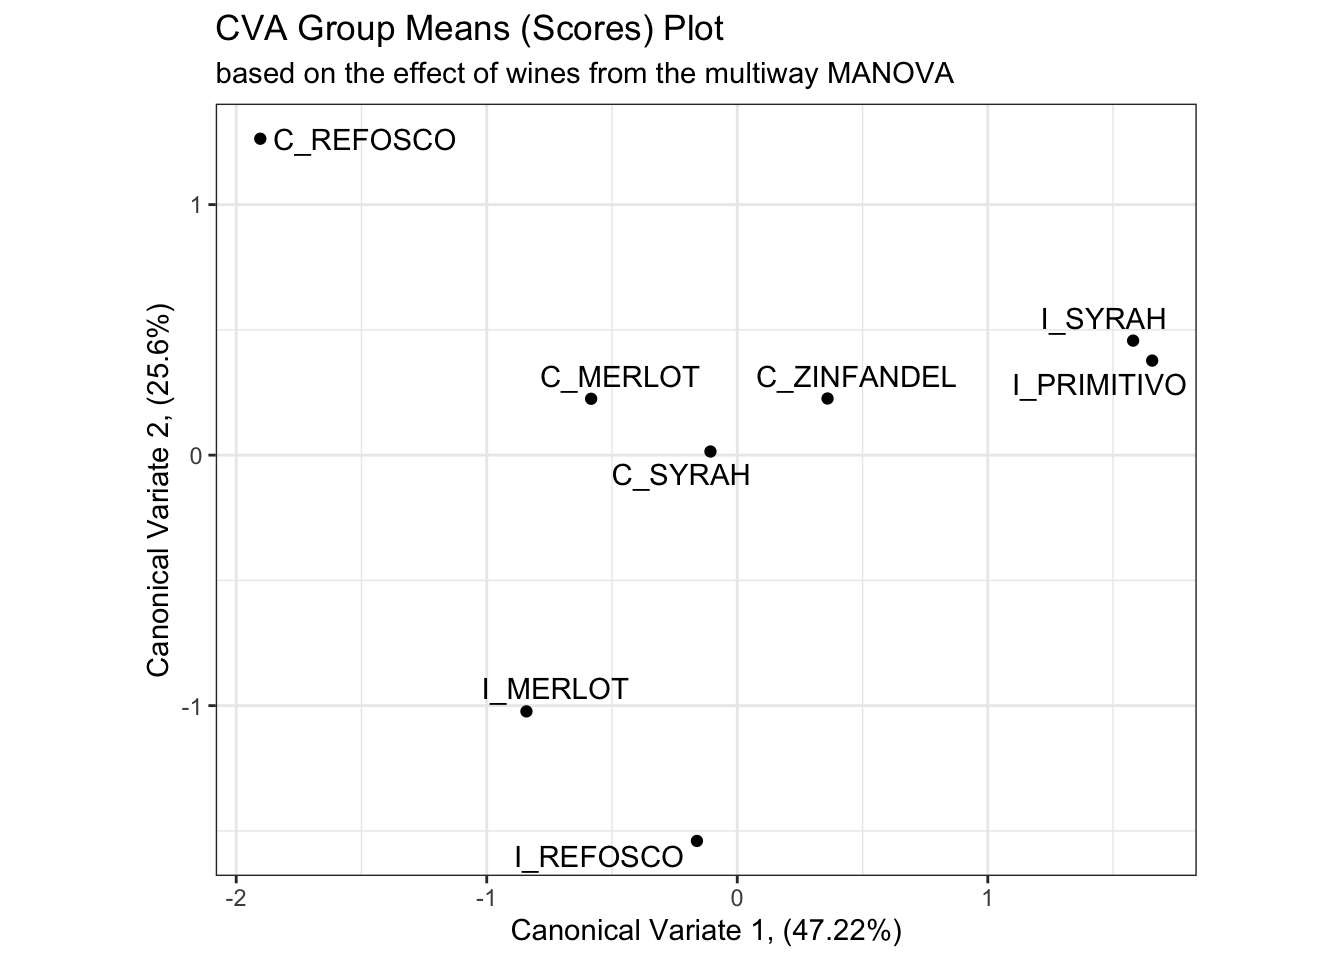
\includegraphics[keepaspectratio]{05-CVA_files/figure-latex/unnamed-chunk-6-2.pdf}}

Besides a reversal of the x-axis (a trivial reflection which does not change meaning), the product mean separation appears to be identical in these two solutions, and the proportion of explained variation remains almost identical. We'll keep up this comparison as we investigate the rest of the solution.

Next, we want to examine how the original variables are related to the resulting ``CVA-space''. This is usually visualized as a vector plot, so we're going to follow convention. This will make our \texttt{ggplot2} calls a little messsier, but I think it is worth it.

In the \texttt{candisc()} output, the \texttt{\$coeffs.raw} list holds the linear combinations of variables that contribute to each dimension:

\begin{Shaded}
\begin{Highlighting}[]
\NormalTok{cva\_res\_oneway}\SpecialCharTok{$}\NormalTok{coeffs.raw }\SpecialCharTok{\%\textgreater{}\%}
  \FunctionTok{round}\NormalTok{(}\DecValTok{2}\NormalTok{) }\SpecialCharTok{\%\textgreater{}\%}
  \FunctionTok{as\_tibble}\NormalTok{(}\AttributeTok{rownames =} \StringTok{"descriptor"}\NormalTok{)}
\end{Highlighting}
\end{Shaded}

\begin{verbatim}
## # A tibble: 20 x 8
##    descriptor       Can1  Can2  Can3  Can4  Can5  Can6  Can7
##    <chr>           <dbl> <dbl> <dbl> <dbl> <dbl> <dbl> <dbl>
##  1 Red_berry        0.01  0.03 -0.04 -0.1  -0.21 -0.06 -0.18
##  2 Dark_berry      -0.12  0.02  0.16  0.05  0.23 -0.03  0.1 
##  3 Jam             -0.22  0.09 -0.05 -0.11 -0.15 -0.03  0.11
##  4 Dried_fruit     -0.06  0.03 -0.1   0.2   0.17  0.03 -0.14
##  5 Artificial_frui -0.18  0.04  0.28 -0.02  0.09 -0.1   0.18
##  6 Chocolate        0.3   0.26  0.1  -0.11 -0.1   0.13  0.07
##  7 Vanilla         -0.03  0.05 -0.18 -0.07 -0.08 -0.05 -0.17
##  8 Oak              0.04  0.1  -0.26  0.15  0    -0.25  0.2 
##  9 Burned           0.32  0.26  0.24 -0.06  0    -0.05  0.05
## 10 Leather         -0.02 -0.22 -0.02 -0.12  0.11 -0.32 -0.07
## 11 Earthy           0.1   0    -0.12 -0.17 -0.01  0.47  0.07
## 12 Spicy            0.02  0.09  0.07  0.06  0.1  -0.22 -0.3 
## 13 Pepper           0.08 -0.09 -0.17  0.27 -0.11  0.12  0.23
## 14 Grassy          -0.31  0     0.16  0.18 -0.09  0.22 -0.16
## 15 Medicinal        0.02 -0.29 -0.02 -0.25 -0.02  0.04  0.15
## 16 Band-aid         0.07 -0.13  0.22  0.05 -0.1  -0.09 -0.16
## 17 Sour            -0.08 -0.07  0.11 -0.05 -0.06 -0.04  0.14
## 18 Bitter           0.02  0.13  0.06  0.06  0.09 -0.04 -0.23
## 19 Alcohol          0.02  0.06 -0.22 -0.28  0.23  0.16 -0.1 
## 20 Astringent       0.1  -0.13  0.11  0.16 -0.06 -0.02  0.02
\end{verbatim}

This tell us that to get an observation's (call it \(i\)) score on Canonical Variate 1, we'd take the following linear sum: \(Can1_i = -0.01*Red\_berry_i + -0.12*Dark\_berry_i + ... + -0.22*Astringent_i\). We do this for every observation to find their score in the space.

To visualize this, rather than plotting the raw coefficients, we typically plot the correlations between the raw coefficients and the original variables, which are stored in the \texttt{\$structure} list. We can consider the ``loadings'' or ``structure coefficients'' themselves as coordinates in the same CVA space, which gives us an idea of how each variable contributes to the dimensions.

\begin{Shaded}
\begin{Highlighting}[]
\NormalTok{cva\_res\_oneway}\SpecialCharTok{$}\NormalTok{structure }\SpecialCharTok{\%\textgreater{}\%}
  \FunctionTok{as\_tibble}\NormalTok{(}\AttributeTok{rownames =} \StringTok{"descriptor"}\NormalTok{) }\SpecialCharTok{\%\textgreater{}\%}
  \FunctionTok{ggplot}\NormalTok{(}\FunctionTok{aes}\NormalTok{(}\AttributeTok{x =}\NormalTok{ Can1, }\AttributeTok{y =}\NormalTok{ Can2)) }\SpecialCharTok{+} 
  \FunctionTok{geom\_segment}\NormalTok{(}\FunctionTok{aes}\NormalTok{(}\AttributeTok{xend =} \DecValTok{0}\NormalTok{, }\AttributeTok{yend =} \DecValTok{0}\NormalTok{), }
               \AttributeTok{arrow =} \FunctionTok{arrow}\NormalTok{(}\AttributeTok{length =} \FunctionTok{unit}\NormalTok{(}\FloatTok{0.2}\NormalTok{, }\AttributeTok{units =} \StringTok{"in"}\NormalTok{), }\AttributeTok{ends =} \StringTok{"first"}\NormalTok{)) }\SpecialCharTok{+}
\NormalTok{  ggrepel}\SpecialCharTok{::}\FunctionTok{geom\_text\_repel}\NormalTok{(}\FunctionTok{aes}\NormalTok{(}\AttributeTok{label =}\NormalTok{ descriptor)) }\SpecialCharTok{+}
  \FunctionTok{labs}\NormalTok{(}\AttributeTok{x =} \FunctionTok{paste0}\NormalTok{(}\StringTok{"Canonical Variate 1, ("}\NormalTok{, }\FunctionTok{round}\NormalTok{(cva\_res\_oneway}\SpecialCharTok{$}\NormalTok{pct[}\DecValTok{1}\NormalTok{], }\DecValTok{2}\NormalTok{), }\StringTok{"\%)"}\NormalTok{),}
       \AttributeTok{y =} \FunctionTok{paste0}\NormalTok{(}\StringTok{"Canonical Variate 2, ("}\NormalTok{, }\FunctionTok{round}\NormalTok{(cva\_res\_oneway}\SpecialCharTok{$}\NormalTok{pct[}\DecValTok{2}\NormalTok{], }\DecValTok{2}\NormalTok{), }\StringTok{"\%)"}\NormalTok{),}
       \AttributeTok{title =} \StringTok{"CVA Loadings Plot"}\NormalTok{,}
       \AttributeTok{subtitle =} \StringTok{"based on the variable loadings from the 1{-}way MANOVA"}\NormalTok{) }\SpecialCharTok{+}
  \FunctionTok{theme\_bw}\NormalTok{()}
\end{Highlighting}
\end{Shaded}

\pandocbounded{\includegraphics[keepaspectratio]{05-CVA_files/figure-latex/unnamed-chunk-8-1.pdf}}

We can see from this plot that the first canonical variate has large positive contributions from ``Burned'' characteristics and smaller contributions from ``Oak'', and strong negative contributions from fruit-related terms like ``Jam'', ``Artificial\_frui {[}sic{]}'', etc. The second canonical variate has large positive contributions from both ``Vanilla'' and ``Chocolate'', and negative contributions from flaw/complex terms like ``Medicinal'', ``Band-aid'', etc.

If we examine the results from the multiway MANOVA we'll see similar results, with the exception of a reversed x-axis (first canonical variate). The main differences seem to be better separation among the fruit-like contributors, with ``Artificial\_frui'' and ``Jam'' being better separated, and an implication that the ``Red\_berry'' and ``Dark\_berry'' attributes are probably contributing more to a higher dimension.

\begin{Shaded}
\begin{Highlighting}[]
\NormalTok{cva\_res}\SpecialCharTok{$}\NormalTok{structure }\SpecialCharTok{\%\textgreater{}\%}
  \FunctionTok{as\_tibble}\NormalTok{(}\AttributeTok{rownames =} \StringTok{"descriptor"}\NormalTok{) }\SpecialCharTok{\%\textgreater{}\%}
  \FunctionTok{ggplot}\NormalTok{(}\FunctionTok{aes}\NormalTok{(}\AttributeTok{x =}\NormalTok{ Can1, }\AttributeTok{y =}\NormalTok{ Can2)) }\SpecialCharTok{+} 
  \FunctionTok{geom\_segment}\NormalTok{(}\FunctionTok{aes}\NormalTok{(}\AttributeTok{xend =} \DecValTok{0}\NormalTok{, }\AttributeTok{yend =} \DecValTok{0}\NormalTok{), }
               \AttributeTok{arrow =} \FunctionTok{arrow}\NormalTok{(}\AttributeTok{length =} \FunctionTok{unit}\NormalTok{(}\FloatTok{0.2}\NormalTok{, }\AttributeTok{units =} \StringTok{"in"}\NormalTok{), }\AttributeTok{ends =} \StringTok{"first"}\NormalTok{)) }\SpecialCharTok{+}
\NormalTok{  ggrepel}\SpecialCharTok{::}\FunctionTok{geom\_text\_repel}\NormalTok{(}\FunctionTok{aes}\NormalTok{(}\AttributeTok{label =}\NormalTok{ descriptor)) }\SpecialCharTok{+}
  \FunctionTok{labs}\NormalTok{(}\AttributeTok{x =} \FunctionTok{paste0}\NormalTok{(}\StringTok{"Canonical Variate 1, ("}\NormalTok{, }\FunctionTok{round}\NormalTok{(cva\_res}\SpecialCharTok{$}\NormalTok{pct[}\DecValTok{1}\NormalTok{], }\DecValTok{2}\NormalTok{), }\StringTok{"\%)"}\NormalTok{),}
       \AttributeTok{y =} \FunctionTok{paste0}\NormalTok{(}\StringTok{"Canonical Variate 2, ("}\NormalTok{, }\FunctionTok{round}\NormalTok{(cva\_res}\SpecialCharTok{$}\NormalTok{pct[}\DecValTok{2}\NormalTok{], }\DecValTok{2}\NormalTok{), }\StringTok{"\%)"}\NormalTok{),}
       \AttributeTok{title =} \StringTok{"CVA Loadings Plot"}\NormalTok{,}
       \AttributeTok{subtitle =} \StringTok{"based on the variable loadings from the multiway MANOVA"}\NormalTok{) }\SpecialCharTok{+}
  \FunctionTok{theme\_bw}\NormalTok{()}
\end{Highlighting}
\end{Shaded}

\pandocbounded{\includegraphics[keepaspectratio]{05-CVA_files/figure-latex/unnamed-chunk-9-1.pdf}}

\subsection{An aside on exporting R plots}\label{an-aside-on-exporting-r-plots}

In the original \textbf{R Opus}, HGH used RStudio's ``Export'' pane to get files from the \texttt{Plots} pane to a format that could be edited in PowerPoint. I tend to discourage this approach, because it produces overall lower resolution results. In addition, as you will have noticed I use \texttt{ggplot2} almost exclusively for visualizations, and the \texttt{ggplot2::ggsave()} function gives easy functional access to \texttt{R}'s somewhat byzantine \texttt{device} interface, making saving images directly much more feasible.

To use \texttt{ggsave()}, you can either save an executed \texttt{ggplot2} plot as an object and pass it to the function, or let the default \texttt{ggsave(plot\ =\ last\_plot())} behavior grab the current visual you're looking at in the \texttt{Plots} pane. Either way, you then need to specify a destination file \emph{with extension} (e.g., \texttt{/path/to/your/image.png}), which \texttt{ggsave()} will parse to get the correct output format. I tend to output as \texttt{.png}, but you might also want to output \texttt{.jpg} or \texttt{.tif}, depending on the usecase. Use \texttt{?ggsave} for more details.

You will also need to specify arguments for \texttt{height\ =} and \texttt{width\ =}, as well as a \texttt{units\ =}, which takes a character string indicating pixels, inches, centimeters, etc. Finally, the \texttt{scale\ =} argument is equivalent to the base \texttt{R} \texttt{cex\ =} arguments: it dictates the degree to which the plot will be ``zoomed''. \texttt{scale\ =} values that are greather than 1 will cause the plot to ``zoom out'' (elements in the plot will appear smaller), and values less than 1 will cause a ``zoom in'' effect.

An example of this workflow, the following (not executed) code will take the last plot of the CVA loadings for the multiway ANOVA, save it as an object called \texttt{p}, and then save that plot to my home folder:

\begin{Shaded}
\begin{Highlighting}[]
\NormalTok{p }\OtherTok{\textless{}{-}}
\NormalTok{  cva\_res}\SpecialCharTok{$}\NormalTok{structure }\SpecialCharTok{\%\textgreater{}\%}
  \FunctionTok{as\_tibble}\NormalTok{(}\AttributeTok{rownames =} \StringTok{"descriptor"}\NormalTok{) }\SpecialCharTok{\%\textgreater{}\%}
  \FunctionTok{ggplot}\NormalTok{(}\FunctionTok{aes}\NormalTok{(}\AttributeTok{x =}\NormalTok{ Can1, }\AttributeTok{y =}\NormalTok{ Can2)) }\SpecialCharTok{+} 
  \FunctionTok{geom\_segment}\NormalTok{(}\FunctionTok{aes}\NormalTok{(}\AttributeTok{xend =} \DecValTok{0}\NormalTok{, }\AttributeTok{yend =} \DecValTok{0}\NormalTok{), }
               \AttributeTok{arrow =} \FunctionTok{arrow}\NormalTok{(}\AttributeTok{length =} \FunctionTok{unit}\NormalTok{(}\FloatTok{0.2}\NormalTok{, }\AttributeTok{units =} \StringTok{"in"}\NormalTok{), }\AttributeTok{ends =} \StringTok{"first"}\NormalTok{)) }\SpecialCharTok{+}
\NormalTok{  ggrepel}\SpecialCharTok{::}\FunctionTok{geom\_text\_repel}\NormalTok{(}\FunctionTok{aes}\NormalTok{(}\AttributeTok{label =}\NormalTok{ descriptor)) }\SpecialCharTok{+}
  \FunctionTok{labs}\NormalTok{(}\AttributeTok{x =} \FunctionTok{paste0}\NormalTok{(}\StringTok{"Canonical Variate 1, ("}\NormalTok{, }\FunctionTok{round}\NormalTok{(cva\_res}\SpecialCharTok{$}\NormalTok{pct[}\DecValTok{1}\NormalTok{], }\DecValTok{2}\NormalTok{), }\StringTok{"\%)"}\NormalTok{),}
       \AttributeTok{y =} \FunctionTok{paste0}\NormalTok{(}\StringTok{"Canonical Variate 2, ("}\NormalTok{, }\FunctionTok{round}\NormalTok{(cva\_res}\SpecialCharTok{$}\NormalTok{pct[}\DecValTok{2}\NormalTok{], }\DecValTok{2}\NormalTok{), }\StringTok{"\%)"}\NormalTok{),}
       \AttributeTok{title =} \StringTok{"CVA Loadings Plot"}\NormalTok{,}
       \AttributeTok{subtitle =} \StringTok{"based on the variable loadings from the multiway MANOVA"}\NormalTok{) }\SpecialCharTok{+}
  \FunctionTok{theme\_bw}\NormalTok{()}

\FunctionTok{ggsave}\NormalTok{(}\AttributeTok{filename =} \StringTok{"\textasciitilde{}/my\_new\_plot.png"}\NormalTok{, }
       \AttributeTok{plot =}\NormalTok{ p, }\AttributeTok{height =} \DecValTok{6}\NormalTok{, }\AttributeTok{width =} \DecValTok{8}\NormalTok{, }
       \AttributeTok{units =} \StringTok{"in"}\NormalTok{, }\AttributeTok{scale =} \FloatTok{1.2}\NormalTok{)}
\end{Highlighting}
\end{Shaded}

\section{Plotting uncertainty in CVA}\label{plotting-uncertainty-in-cva}

One of the advantages of CVA is that it is based on raw data, which PCA is \emph{typically} not \citep[an exception is so-called Tucker-1 PCA,][]{dettmarPrincipal2020}. So far we've only visualized the \emph{group} means for the wines in our CVA plots, but we can investigate the \texttt{\$scores} data frame in the CVA results to see the raw observation scores, and use them to plot confidence ellipses.

\begin{Shaded}
\begin{Highlighting}[]
\NormalTok{cva\_res\_oneway}\SpecialCharTok{$}\NormalTok{scores }\SpecialCharTok{\%\textgreater{}\%} 
  \FunctionTok{as\_tibble}\NormalTok{()}
\end{Highlighting}
\end{Shaded}

\begin{verbatim}
## # A tibble: 336 x 8
##    ProductName   Can1   Can2   Can3   Can4     Can5   Can6    Can7
##    <fct>        <dbl>  <dbl>  <dbl>  <dbl>    <dbl>  <dbl>   <dbl>
##  1 C_MERLOT     0.378  1.23  -2.16   1.33   1.25    -0.177 -1.38  
##  2 C_SYRAH     -1.43  -0.233  0.130 -1.97  -0.577   -1.42   0.478 
##  3 C_ZINFANDEL -0.499 -0.177 -1.58   1.38  -0.00298 -0.807 -0.0839
##  4 C_REFOSCO   -0.352  3.45   0.848 -2.56  -1.22    -0.368  0.740 
##  5 I_MERLOT     0.882 -1.40   2.42   0.508  0.715    0.535  0.153 
##  6 I_SYRAH     -2.34   2.32   0.679 -1.85   0.0947  -1.17  -1.81  
##  7 I_PRIMITIVO -3.27   1.06   0.445 -0.766 -1.51    -1.44   1.60  
##  8 I_REFOSCO    0.881 -0.986  1.14  -2.60  -0.0514  -1.25   1.56  
##  9 C_MERLOT     2.39   1.16   0.794  0.678 -0.340   -0.469  1.06  
## 10 C_SYRAH      1.95   0.928 -1.09   0.847  1.01     0.644 -0.155 
## # i 326 more rows
\end{verbatim}

\begin{Shaded}
\begin{Highlighting}[]
\NormalTok{cva\_res}\SpecialCharTok{$}\NormalTok{scores }\SpecialCharTok{\%\textgreater{}\%}
  \FunctionTok{as\_tibble}\NormalTok{()}
\end{Highlighting}
\end{Shaded}

\begin{verbatim}
## # A tibble: 336 x 10
##    ProductName NJ    NR      Can1   Can2   Can3    Can4    Can5   Can6    Can7
##    <fct>       <fct> <fct>  <dbl>  <dbl>  <dbl>   <dbl>   <dbl>  <dbl>   <dbl>
##  1 C_MERLOT    1331  7     -0.478  1.14  -0.778 -0.633  -2.51   -1.06   2.46  
##  2 C_SYRAH     1331  7      3.53   0.810  4.58  -2.30    0.403  -2.94   0.312 
##  3 C_ZINFANDEL 1331  7     -0.551  0.137 -0.675  0.0954 -1.37   -2.47   0.864 
##  4 C_REFOSCO   1331  7      2.19   5.17   4.06  -1.05    1.40   -0.988  0.209 
##  5 I_MERLOT    1331  7     -3.59  -1.79   4.29   0.980  -2.15   -0.613 -0.0964
##  6 I_SYRAH     1331  7      5.89   2.58   4.66  -0.838  -0.0944 -1.30   3.14  
##  7 I_PRIMITIVO 1331  7      5.28   2.20   3.59   1.27    2.51   -2.61  -1.12  
##  8 I_REFOSCO   1331  7     -1.73  -0.271  5.68  -0.973   1.75   -1.96  -0.896 
##  9 C_MERLOT    1400  7     -3.98   2.69  -0.498  0.0528 -0.804  -1.02  -1.57  
## 10 C_SYRAH     1400  7     -3.49   1.72  -1.04  -1.39   -2.38   -0.338  0.563 
## # i 326 more rows
\end{verbatim}

We can add these to our mean-scores plots using the \texttt{ggplot2} layering capabilities--another example of using \texttt{ggplot2} over base R graphics.

\begin{Shaded}
\begin{Highlighting}[]
\NormalTok{scores\_p\_1 }\SpecialCharTok{+} 
  \FunctionTok{stat\_ellipse}\NormalTok{(}\AttributeTok{data =}\NormalTok{ cva\_res\_oneway}\SpecialCharTok{$}\NormalTok{scores,}
               \AttributeTok{mapping =} \FunctionTok{aes}\NormalTok{(}\AttributeTok{group =}\NormalTok{ ProductName),}
               \AttributeTok{type =} \StringTok{"t"}\NormalTok{) }\SpecialCharTok{+}
  \FunctionTok{coord\_fixed}\NormalTok{()}
\end{Highlighting}
\end{Shaded}

\begin{verbatim}
## Coordinate system already present. Adding new coordinate system, which will
## replace the existing one.
\end{verbatim}

\pandocbounded{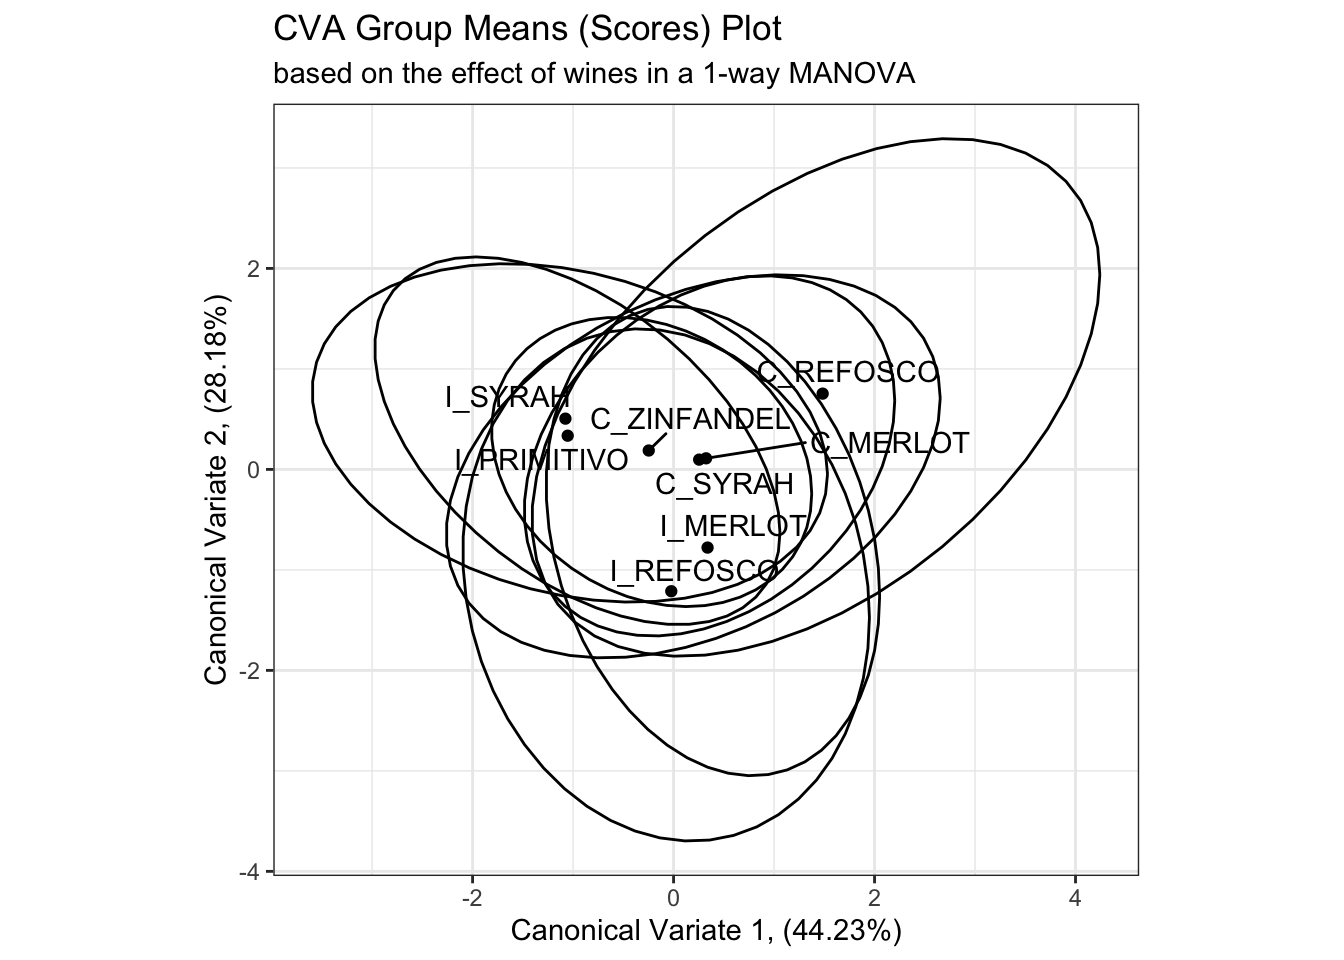
\includegraphics[keepaspectratio]{05-CVA_files/figure-latex/unnamed-chunk-12-1.pdf}}

\begin{Shaded}
\begin{Highlighting}[]
\CommentTok{\# This is in some contrast to the original R Opus, in which HGH used 95\% confidence circles}

\NormalTok{scores\_p\_1 }\SpecialCharTok{+}
  \FunctionTok{stat\_ellipse}\NormalTok{(}\AttributeTok{data =}\NormalTok{ cva\_res\_oneway}\SpecialCharTok{$}\NormalTok{scores,}
               \AttributeTok{mapping =} \FunctionTok{aes}\NormalTok{(}\AttributeTok{group =}\NormalTok{ ProductName),}
               \AttributeTok{type =} \StringTok{"euclid"}\NormalTok{,}
               \AttributeTok{level =} \DecValTok{2} \SpecialCharTok{/} \FunctionTok{sqrt}\NormalTok{(}\FunctionTok{table}\NormalTok{(cva\_res\_oneway}\SpecialCharTok{$}\NormalTok{scores[,}\DecValTok{1}\NormalTok{]))[}\DecValTok{1}\NormalTok{]) }\SpecialCharTok{+} 
  \FunctionTok{coord\_fixed}\NormalTok{()}
\end{Highlighting}
\end{Shaded}

\begin{verbatim}
## Coordinate system already present. Adding new coordinate system, which will
## replace the existing one.
\end{verbatim}

\pandocbounded{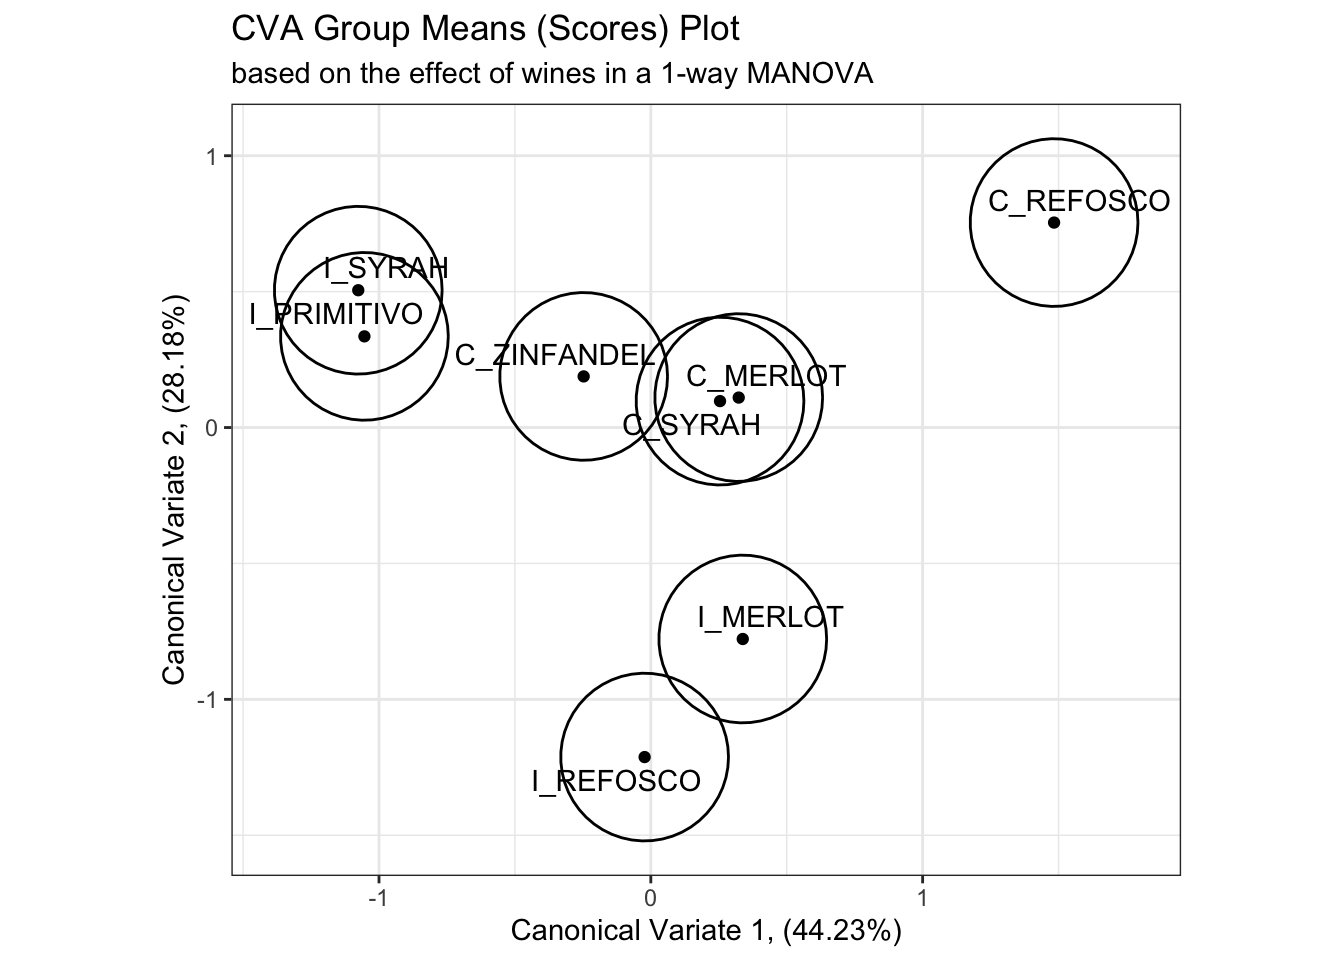
\includegraphics[keepaspectratio]{05-CVA_files/figure-latex/unnamed-chunk-12-2.pdf}}

While I don't have immediate access to the original reference HGH cites, the calculation provided in the original \textbf{R Opus} and repeated above draws a circle of confidence based on the number of observations in each group, which to my mind seems likely to underestimate the overlap between samples. On the other hand, my simple confidence ellipses are for the raw observations, rather than the ``barycentric'' (mean vector) confidence intervals that the method given by HGH hopes to provide. We can look at this by looking at the actual observations plotted in the CVA space.

\begin{Shaded}
\begin{Highlighting}[]
\NormalTok{scores\_p\_1 }\SpecialCharTok{+}
  \FunctionTok{geom\_point}\NormalTok{(}\AttributeTok{data =}\NormalTok{ cva\_res\_oneway}\SpecialCharTok{$}\NormalTok{scores,}
             \FunctionTok{aes}\NormalTok{(}\AttributeTok{color =}\NormalTok{ ProductName),}
             \AttributeTok{alpha =} \DecValTok{1}\SpecialCharTok{/}\DecValTok{3}\NormalTok{) }\SpecialCharTok{+}
  \FunctionTok{stat\_ellipse}\NormalTok{(}\AttributeTok{data =}\NormalTok{ cva\_res\_oneway}\SpecialCharTok{$}\NormalTok{scores,}
               \AttributeTok{mapping =} \FunctionTok{aes}\NormalTok{(}\AttributeTok{fill =}\NormalTok{ ProductName), }
               \AttributeTok{geom =} \StringTok{"polygon"}\NormalTok{,}
               \AttributeTok{alpha =} \FloatTok{0.1}\NormalTok{) }\SpecialCharTok{+}
  \FunctionTok{stat\_ellipse}\NormalTok{(}\AttributeTok{data =}\NormalTok{ cva\_res\_oneway}\SpecialCharTok{$}\NormalTok{scores,}
               \AttributeTok{mapping =} \FunctionTok{aes}\NormalTok{(}\AttributeTok{group =}\NormalTok{ ProductName, }\AttributeTok{color =}\NormalTok{ ProductName),}
               \AttributeTok{type =} \StringTok{"euclid"}\NormalTok{,}
               \AttributeTok{level =} \DecValTok{2} \SpecialCharTok{/} \FunctionTok{sqrt}\NormalTok{(}\FunctionTok{table}\NormalTok{(cva\_res\_oneway}\SpecialCharTok{$}\NormalTok{scores[,}\DecValTok{1}\NormalTok{]))[}\DecValTok{1}\NormalTok{]) }\SpecialCharTok{+}
  \FunctionTok{coord\_fixed}\NormalTok{()}
\end{Highlighting}
\end{Shaded}

\begin{verbatim}
## Coordinate system already present. Adding new coordinate system, which will
## replace the existing one.
\end{verbatim}

\pandocbounded{\includegraphics[keepaspectratio]{05-CVA_files/figure-latex/unnamed-chunk-13-1.pdf}}

When we plot the actual observations, it is apparent that the proposed confidence circles don't do a good job of capturing the observed variability in the data. They are probably overgenerous in their estimation of the separability of the individual observations, as from what I can tell the radius of the circles is simply a function of the number of observations. This would decrease as the number of observations go up, which makes sense as more observations will give more stable mean vectors, but it doesn't really take advantage of the raw data. On the other hand, the confidence intervals based on raw observations (which are no longer barycentric) don't tell us much about mean separation--they are more akin to predicting the orientation of other new observations for each wine in the CVA space.

In the original \textbf{R Opus}, HGH provides a function from Helene Hopfer, Peter Buffon, and Vince Buffalo to calculate barycentric confidence ellipses based on, I believe, a similar method as that given in \citet{peltierCanonical2015}. These functions rely on assumptions of bivariate normality for mean scores on the represented CVA axes, which is reasonable, but I think the function is quite opaque. As noted in \citet{peltierCanonical2015}, a resampling approach could be used, so we're going to take this approach to illustrate such an approach. Resampling, which involves perturbing the original data randomly and then examining its stability, is a nonparametric approach that is useful because it makes very few assumptions about either our data or analysis.

\begin{Shaded}
\begin{Highlighting}[]
\CommentTok{\# This is still going to be a bit complicated, but I will walk through the steps}
\CommentTok{\# in my thinking.}


\CommentTok{\# First, we will write two functions that just calculate the canonical variate}
\CommentTok{\# scores for the means of our data.  These are based on the equations from}
\CommentTok{\# Rencher 2002.}
\NormalTok{get\_cva\_1 }\OtherTok{\textless{}{-}} \ControlFlowTok{function}\NormalTok{(means)\{}
  
\NormalTok{  cva\_res\_oneway}\SpecialCharTok{$}\NormalTok{coeffs.raw[, }\DecValTok{1}\NormalTok{] }\SpecialCharTok{\%*\%}\NormalTok{ means}
  
\NormalTok{\}}

\NormalTok{get\_cva\_2 }\OtherTok{\textless{}{-}} \ControlFlowTok{function}\NormalTok{(means)\{}
  
\NormalTok{  cva\_res\_oneway}\SpecialCharTok{$}\NormalTok{coeffs.raw[, }\DecValTok{2}\NormalTok{] }\SpecialCharTok{\%*\%}\NormalTok{ means}
  
\NormalTok{\}}

\CommentTok{\# Then, we write a convenience function that will resample our data with}
\CommentTok{\# replacement, calculate centered means for our samples, and then project them}
\CommentTok{\# into our original CVA space using the convenience functions we wrote above.}
\NormalTok{get\_bootstrapped\_means }\OtherTok{\textless{}{-}} \ControlFlowTok{function}\NormalTok{()\{}
  
\NormalTok{  descriptive\_data }\SpecialCharTok{\%\textgreater{}\%}
  \FunctionTok{select}\NormalTok{(}\SpecialCharTok{{-}}\NormalTok{NJ, }\SpecialCharTok{{-}}\NormalTok{NR) }\SpecialCharTok{\%\textgreater{}\%}
  \FunctionTok{group\_by}\NormalTok{(ProductName) }\SpecialCharTok{\%\textgreater{}\%}
    \CommentTok{\# Here we resample each wine {-} we draw 42 new observations for each wine}
    \CommentTok{\# with replacement}
  \FunctionTok{slice\_sample}\NormalTok{(}\AttributeTok{prop =} \DecValTok{1}\NormalTok{, }\AttributeTok{replace =} \ConstantTok{TRUE}\NormalTok{) }\SpecialCharTok{\%\textgreater{}\%}
    \CommentTok{\# We calculate the mean for the newly drawn samples}
  \FunctionTok{summarize\_if}\NormalTok{(is.numeric, }\SpecialCharTok{\textasciitilde{}}\FunctionTok{mean}\NormalTok{(.)) }\SpecialCharTok{\%\textgreater{}\%} 
    \CommentTok{\# And then we center the means (by subtracting the column means)}
  \FunctionTok{mutate\_if}\NormalTok{(is.numeric, }\SpecialCharTok{\textasciitilde{}}\NormalTok{. }\SpecialCharTok{{-}} \FunctionTok{mean}\NormalTok{(.)) }\SpecialCharTok{\%\textgreater{}\%}
    \CommentTok{\# Finally, we apply our projection functions (the linear combinations from}
    \CommentTok{\# our CVA) to project the bootstrapped means into our new space}
  \FunctionTok{nest}\NormalTok{(}\AttributeTok{data =} \SpecialCharTok{{-}}\NormalTok{ProductName) }\SpecialCharTok{\%\textgreater{}\%}
  \FunctionTok{mutate}\NormalTok{(}\AttributeTok{means =} \FunctionTok{map}\NormalTok{(data, }\SpecialCharTok{\textasciitilde{}}\FunctionTok{as.matrix}\NormalTok{(.x) }\SpecialCharTok{\%\textgreater{}\%} \FunctionTok{t}\NormalTok{()),}
         \AttributeTok{Can1 =} \FunctionTok{map\_dbl}\NormalTok{(means, }\SpecialCharTok{\textasciitilde{}}\FunctionTok{get\_cva\_1}\NormalTok{(.x)),}
         \AttributeTok{Can2 =} \FunctionTok{map\_dbl}\NormalTok{(means, }\SpecialCharTok{\textasciitilde{}}\FunctionTok{get\_cva\_2}\NormalTok{(.x)),}
\NormalTok{         ) }\SpecialCharTok{\%\textgreater{}\%}
    \FunctionTok{select}\NormalTok{(ProductName, Can1, Can2)}
  
\NormalTok{\}}

\CommentTok{\# For example, here is the result of our function}
\FunctionTok{get\_bootstrapped\_means}\NormalTok{()}
\end{Highlighting}
\end{Shaded}

\begin{verbatim}
## # A tibble: 8 x 3
##   ProductName    Can1    Can2
##   <fct>         <dbl>   <dbl>
## 1 C_MERLOT     0.398  -0.0316
## 2 C_REFOSCO    1.77    0.768 
## 3 C_SYRAH     -0.0148 -0.138 
## 4 C_ZINFANDEL -0.346   0.227 
## 5 I_MERLOT     0.201  -0.681 
## 6 I_PRIMITIVO -1.01    0.178 
## 7 I_REFOSCO   -0.141  -0.973 
## 8 I_SYRAH     -0.856   0.650
\end{verbatim}

\begin{Shaded}
\begin{Highlighting}[]
\CommentTok{\# In order to generate a set of resampled confidence ellipses for our results,}
\CommentTok{\# we\textquotesingle{}ll run this 100 times for speed (for accuracy, 1000x would be better) and use}
\CommentTok{\# stat\_ellipse() to draw those.}

\NormalTok{bootstrapped\_cva\_means }\OtherTok{\textless{}{-}} 
  \FunctionTok{tibble}\NormalTok{(}\AttributeTok{boot\_id =} \DecValTok{1}\SpecialCharTok{:}\DecValTok{100}\NormalTok{) }\SpecialCharTok{\%\textgreater{}\%}
  \FunctionTok{mutate}\NormalTok{(}\AttributeTok{bootstrapped\_data =} \FunctionTok{map}\NormalTok{(boot\_id, }\SpecialCharTok{\textasciitilde{}}\FunctionTok{get\_bootstrapped\_means}\NormalTok{())) }\SpecialCharTok{\%\textgreater{}\%}
  \FunctionTok{unnest}\NormalTok{(bootstrapped\_data)}

\NormalTok{scores\_p\_1 }\SpecialCharTok{+} 
  \FunctionTok{stat\_ellipse}\NormalTok{(}\AttributeTok{data =}\NormalTok{ bootstrapped\_cva\_means,}
               \FunctionTok{aes}\NormalTok{(}\AttributeTok{fill =}\NormalTok{ ProductName),}
               \AttributeTok{geom =} \StringTok{"polygon"}\NormalTok{,}
               \AttributeTok{alpha =} \FloatTok{0.1}\NormalTok{) }\SpecialCharTok{+}
  \FunctionTok{coord\_fixed}\NormalTok{() }\SpecialCharTok{+} 
  \FunctionTok{theme}\NormalTok{(}\AttributeTok{legend.position =} \StringTok{"none"}\NormalTok{)}
\end{Highlighting}
\end{Shaded}

\begin{verbatim}
## Coordinate system already present. Adding new coordinate system, which will
## replace the existing one.
\end{verbatim}

\pandocbounded{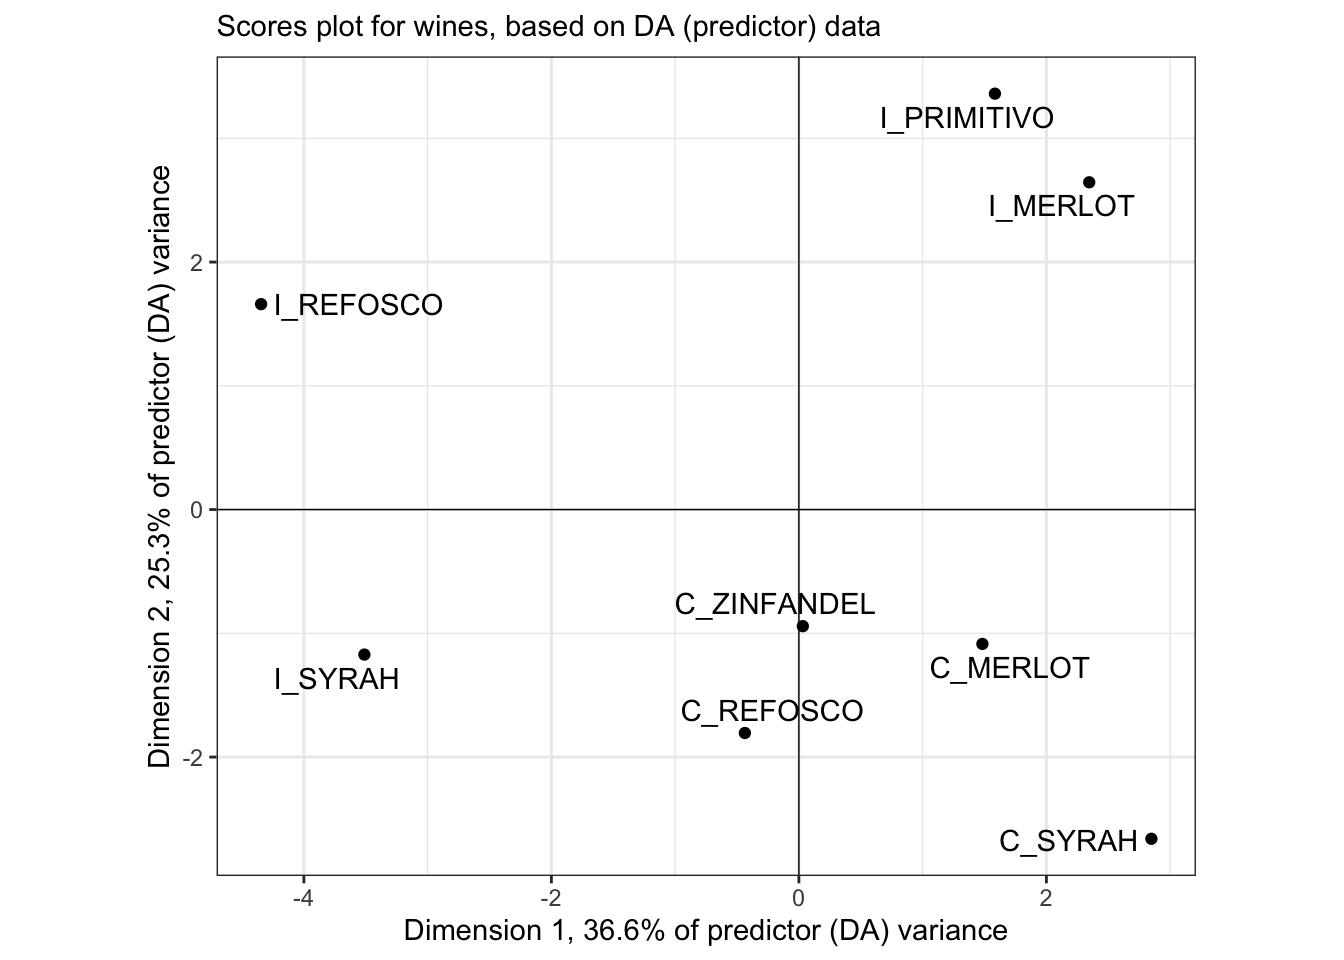
\includegraphics[keepaspectratio]{05-CVA_files/figure-latex/unnamed-chunk-14-1.pdf}}

While this requires a bit of computation time (around 5 seconds on my M2 Mac Mini, writing in 2024), this is still pretty tractable. It would take about 1 minute to do a ``publishable'' bootstrap of 1000 samples, which is still fine. As we'll see, this resampling approach will generalize easily to other needs.

This is a more conservative result than that given by the bivariate normal ellipses in the original \textbf{R Opus}, although the actual conclusions of pairwise sample discrimination are identical.

\section{Packages used in this chapter}\label{packages-used-in-this-chapter-4}

\begin{Shaded}
\begin{Highlighting}[]
\FunctionTok{sessionInfo}\NormalTok{()}
\end{Highlighting}
\end{Shaded}

\begin{verbatim}
## R version 4.4.1 (2024-06-14)
## Platform: x86_64-apple-darwin20
## Running under: macOS 15.2
## 
## Matrix products: default
## BLAS:   /Library/Frameworks/R.framework/Versions/4.4-x86_64/Resources/lib/libRblas.0.dylib 
## LAPACK: /Library/Frameworks/R.framework/Versions/4.4-x86_64/Resources/lib/libRlapack.dylib;  LAPACK version 3.12.0
## 
## locale:
## [1] en_US.UTF-8/en_US.UTF-8/en_US.UTF-8/C/en_US.UTF-8/en_US.UTF-8
## 
## time zone: America/New_York
## tzcode source: internal
## 
## attached base packages:
## [1] stats     graphics  grDevices datasets  utils     methods   base     
## 
## other attached packages:
##  [1] here_1.0.1      candisc_0.9.0   heplots_1.7.3   broom_1.0.6    
##  [5] lubridate_1.9.3 forcats_1.0.0   stringr_1.5.1   dplyr_1.1.4    
##  [9] purrr_1.0.2     readr_2.1.5     tidyr_1.3.1     tibble_3.2.1   
## [13] ggplot2_3.5.1   tidyverse_2.0.0 rgl_1.3.14     
## 
## loaded via a namespace (and not attached):
##  [1] utf8_1.2.4        generics_0.1.3    renv_1.0.9        stringi_1.8.4    
##  [5] hms_1.1.3         digest_0.6.37     magrittr_2.0.3    evaluate_0.23    
##  [9] grid_4.4.1        timechange_0.3.0  bookdown_0.39     fastmap_1.2.0    
## [13] rprojroot_2.0.4   jsonlite_1.8.8    ggrepel_0.9.5     backports_1.5.0  
## [17] fansi_1.0.6       scales_1.3.0      abind_1.4-5       cli_3.6.3        
## [21] crayon_1.5.2      rlang_1.1.4       bit64_4.0.5       munsell_0.5.1    
## [25] base64enc_0.1-3   withr_3.0.0       yaml_2.3.8        parallel_4.4.1   
## [29] tools_4.4.1       tzdb_0.4.0        colorspace_2.1-0  vctrs_0.6.5      
## [33] R6_2.5.1          lifecycle_1.0.4   bit_4.0.5         car_3.1-2        
## [37] htmlwidgets_1.6.4 vroom_1.6.5       MASS_7.3-60.2     pkgconfig_2.0.3  
## [41] pillar_1.9.0      gtable_0.3.5      Rcpp_1.0.13       glue_1.7.0       
## [45] highr_0.10        xfun_0.49         tidyselect_1.2.1  rstudioapi_0.16.0
## [49] knitr_1.46        farver_2.1.2      htmltools_0.5.8.1 labeling_0.4.3   
## [53] rmarkdown_2.27    carData_3.0-5     compiler_4.4.1
\end{verbatim}

\chapter{Principal Components Analysis (PCA)}\label{principal-components-analysis-pca}

While HGH is a strong proponent of Canonical Variate Analysis (CVA), it is hard to argue that Principal Components Analysis is not the ``workhorse'' tool for analysis of multivariate sensory datasets. In fact, PCA is probably the most common tool for multivariate analysis, hard stop. This is because it is so closely related to eigendecomposition and Singular Value Decomposition (SVD).

We'll start with setting up our data as usual. This time, we'll use the \texttt{FactoMineR} package for PCA because of its comprehensive outputs. You could also use the base \texttt{R} function \texttt{princomp()}, but it provides fewer sensory-specific options.

\begin{Shaded}
\begin{Highlighting}[]
\FunctionTok{library}\NormalTok{(tidyverse)}
\FunctionTok{library}\NormalTok{(FactoMineR) }\CommentTok{\# this is new}
\FunctionTok{library}\NormalTok{(here)}

\NormalTok{descriptive\_data }\OtherTok{\textless{}{-}} 
  \FunctionTok{read\_csv}\NormalTok{(}\FunctionTok{here}\NormalTok{(}\StringTok{"data/torriDAFinal.csv"}\NormalTok{)) }\SpecialCharTok{\%\textgreater{}\%}
  \CommentTok{\# note the use of across() to mutate multiple columns}
  \FunctionTok{mutate}\NormalTok{(}\FunctionTok{across}\NormalTok{(}\AttributeTok{.cols =} \DecValTok{1}\SpecialCharTok{:}\DecValTok{3}\NormalTok{, }\SpecialCharTok{\textasciitilde{}}\FunctionTok{as.factor}\NormalTok{(.)))}
\end{Highlighting}
\end{Shaded}

\section{What does PCA do?}\label{what-does-pca-do}

As a reminder, in a dataset with multiple variables measured on the same observations, PCA finds \emph{linear combinations} of the original variables that maximally explain the covariance among the original variables. Thus, the criterion maximized by PCA is explanation of (co)variance. We often describe this as ``amount of variation explained'' by the subsequent, new linear combinations. In highly correlated data, which is usually the case in sensory data, PCA is very effective at finding a few new linear combinations of the original variables that explain most of the observed variance.

Typically, PCA is conducted on mean vectors.

Speaking of CVA, recall that CVA finds linear combinations of variables that best explain \emph{mean-vector} separation in the original data. Thus, while CVA operates on raw data, it is looking to separate the mean-vectors or ``barycenters'' of the data. PCA ``knows'' less information about the data: in fact, PCA is an ``unsupervised'' learning approach, in comparison to the ``supervision'' provided by the group IDs in CVA. PCA is also generally lax about assumptions: the main assumption is that the observed variables are continuous. If they are categorical, it is probably more appropriate to use (multiple) Correspondence Analysis.

PCA is equivalent to the eigendecomposition of the covariance matrix of our original variables. If we standardize our variables (convert them to \emph{z}-scores, or equivalently center our variables and standardize them to have unit variance) we will be conducting eigendecomposition on a correlation matrix. Thus, you will often see discussion of ``correlation'' vs ``covariance'' PCA. There are times in which one or the other is most appropriate for sensory results, but here we'll focus on correlation PCA.

A final note on PCA is that, because of the nature of eigendecomposition, the components are mutually orthogonal: they are uncorrelated and, geometrically, form right angles in the multivariate space.

For more details on PCA, I strongly recommend Hervé Abdi's excellent and detailed chapter on the topic, \href{https://personal.utdallas.edu/~herve/}{available on his website (I think A77 is the entry in his pub list)}.

\section{Let's do PCA!}\label{lets-do-pca}

HGH starts the original \textbf{R Opus} with a function to take column and group means of the data in \texttt{descriptive\_data} that she calls \texttt{mtable()}, for ``means table''. Luckily for us, this functionality is a basic part of the \texttt{tidyverse}, and we've already used this approach in previous sections. So let's generate a means table using \texttt{tidyverse}:

\begin{Shaded}
\begin{Highlighting}[]
\NormalTok{descriptive\_means }\OtherTok{\textless{}{-}}
\NormalTok{  descriptive\_data }\SpecialCharTok{\%\textgreater{}\%}
  \CommentTok{\# What defines the group for which we want means?}
  \FunctionTok{group\_by}\NormalTok{(ProductName) }\SpecialCharTok{\%\textgreater{}\%}
  \CommentTok{\# Then we take the group means for every numeric variable (ignore NR, NJ)}
  \CommentTok{\# Note the use of where() with across() to use a "predicate" function}
  \FunctionTok{summarize}\NormalTok{(}\FunctionTok{across}\NormalTok{(}\FunctionTok{where}\NormalTok{(is.numeric), }\SpecialCharTok{\textasciitilde{}}\FunctionTok{mean}\NormalTok{(.)))}

\NormalTok{descriptive\_means}
\end{Highlighting}
\end{Shaded}

\begin{verbatim}
## # A tibble: 8 x 21
##   ProductName Red_berry Dark_berry   Jam Dried_fruit Artificial_frui Chocolate
##   <fct>           <dbl>      <dbl> <dbl>       <dbl>           <dbl>     <dbl>
## 1 C_MERLOT         2.46       3.05 1.37         1.86           0.776     1.19 
## 2 C_REFOSCO        2.47       2.46 1.03         1.42           0.924     2.00 
## 3 C_SYRAH          2.46       2.93 1.75         1.68           0.883     1.42 
## 4 C_ZINFANDEL      3.08       3.06 1.98         2.06           0.864     0.969
## 5 I_MERLOT         2.79       2.35 0.843        1.85           0.574     0.783
## 6 I_PRIMITIVO      3.85       3.38 3.61         1.44           2.19      1.38 
## 7 I_REFOSCO        2.48       3.01 1.54         1.87           1.11      0.810
## 8 I_SYRAH          3.17       4.48 3.10         2.16           2.43      1.20 
## # i 14 more variables: Vanilla <dbl>, Oak <dbl>, Burned <dbl>, Leather <dbl>,
## #   Earthy <dbl>, Spicy <dbl>, Pepper <dbl>, Grassy <dbl>, Medicinal <dbl>,
## #   `Band-aid` <dbl>, Sour <dbl>, Bitter <dbl>, Alcohol <dbl>, Astringent <dbl>
\end{verbatim}

The \texttt{FactoMineR::PCA()} function is great, but it also tries to do way too much. One of its annoying habits is a desire to give you a lot of plots you don't want. So be sure to use the \texttt{graph\ =\ FALSE} argument so you have more control over plotting. It also uses an older standard which relies on storing observation IDs in \texttt{row.names}--this isn't great programming practice and we have to explicitly do so. Following HGH, we are going to conduct a covariance PCA by setting \texttt{scale.unit\ =\ FALSE}.

\begin{Shaded}
\begin{Highlighting}[]
\NormalTok{means\_pca }\OtherTok{\textless{}{-}} 
\NormalTok{  descriptive\_means }\SpecialCharTok{\%\textgreater{}\%}
  \FunctionTok{column\_to\_rownames}\NormalTok{(}\StringTok{"ProductName"}\NormalTok{) }\SpecialCharTok{\%\textgreater{}\%}
  \FunctionTok{PCA}\NormalTok{(}\AttributeTok{scale.unit =} \ConstantTok{FALSE}\NormalTok{, }\AttributeTok{graph =} \ConstantTok{FALSE}\NormalTok{)}

\NormalTok{means\_pca}
\end{Highlighting}
\end{Shaded}

\begin{verbatim}
## **Results for the Principal Component Analysis (PCA)**
## The analysis was performed on 8 individuals, described by 20 variables
## *The results are available in the following objects:
## 
##    name               description                          
## 1  "$eig"             "eigenvalues"                        
## 2  "$var"             "results for the variables"          
## 3  "$var$coord"       "coord. for the variables"           
## 4  "$var$cor"         "correlations variables - dimensions"
## 5  "$var$cos2"        "cos2 for the variables"             
## 6  "$var$contrib"     "contributions of the variables"     
## 7  "$ind"             "results for the individuals"        
## 8  "$ind$coord"       "coord. for the individuals"         
## 9  "$ind$cos2"        "cos2 for the individuals"           
## 10 "$ind$contrib"     "contributions of the individuals"   
## 11 "$call"            "summary statistics"                 
## 12 "$call$centre"     "mean of the variables"              
## 13 "$call$ecart.type" "standard error of the variables"    
## 14 "$call$row.w"      "weights for the individuals"        
## 15 "$call$col.w"      "weights for the variables"
\end{verbatim}

The nice thing about \texttt{PCA()} is that it gives a well-structured list of results that we can do a lot with. First off, let's make a quick ``scree plot'', describing the variance explained by each of the principal components.

\begin{Shaded}
\begin{Highlighting}[]
\CommentTok{\# Here are the actual numeric results.}
\NormalTok{means\_pca}\SpecialCharTok{$}\NormalTok{eig}
\end{Highlighting}
\end{Shaded}

\begin{verbatim}
##        eigenvalue percentage of variance cumulative percentage of variance
## comp 1 2.65480006              50.496451                          50.49645
## comp 2 1.24849044              23.747301                          74.24375
## comp 3 0.53223903              10.123618                          84.36737
## comp 4 0.32433613               6.169136                          90.53651
## comp 5 0.31577131               6.006227                          96.54273
## comp 6 0.12584413               2.393657                          98.93639
## comp 7 0.05591818               1.063609                         100.00000
\end{verbatim}

\begin{Shaded}
\begin{Highlighting}[]
\CommentTok{\# And now we can plot}
\NormalTok{means\_pca}\SpecialCharTok{$}\NormalTok{eig }\SpecialCharTok{\%\textgreater{}\%}
  \CommentTok{\# Note that we need to use \textasciigrave{}rownames=\textasciigrave{} to capture the rownames from PCA()}
  \FunctionTok{as\_tibble}\NormalTok{(}\AttributeTok{rownames =} \StringTok{"component"}\NormalTok{) }\SpecialCharTok{\%\textgreater{}\%}
  \FunctionTok{ggplot}\NormalTok{(}\FunctionTok{aes}\NormalTok{(}\AttributeTok{x =}\NormalTok{ component, }\AttributeTok{y =} \StringTok{\textasciigrave{}}\AttributeTok{percentage of variance}\StringTok{\textasciigrave{}}\NormalTok{, }\AttributeTok{group =} \DecValTok{1}\NormalTok{)) }\SpecialCharTok{+} 
  \FunctionTok{geom\_line}\NormalTok{() }\SpecialCharTok{+}
  \FunctionTok{theme\_bw}\NormalTok{()}
\end{Highlighting}
\end{Shaded}

\pandocbounded{\includegraphics[keepaspectratio]{06-PCA_files/figure-latex/unnamed-chunk-4-1.pdf}}

We can see that the ``elbow'' here occurs at the third or fourth component, but we're going to only examine the first 2 components. Keep in mind that this means some variation might not be apparent.

The so-called ``loadings'' in a PCA are the weights of the linear combination of original variables that make up each component. We access them in the \texttt{\$var\$coord} table in the results from \texttt{PCA()}.

\begin{Shaded}
\begin{Highlighting}[]
\NormalTok{means\_pca}\SpecialCharTok{$}\NormalTok{var}\SpecialCharTok{$}\NormalTok{coord}
\end{Highlighting}
\end{Shaded}

\begin{verbatim}
##                        Dim.1       Dim.2        Dim.3         Dim.4
## Red_berry        0.392823276  0.01215638 -0.121346852  0.0825451624
## Dark_berry       0.520232898  0.08267522  0.199523469 -0.1864158541
## Jam              0.888495244  0.04433424  0.073820850  0.1720938632
## Dried_fruit      0.050212647  0.10009820 -0.019690630 -0.1664223919
## Artificial_frui  0.572309456  0.05751255  0.238851293 -0.0038853644
## Chocolate       -0.003475125 -0.30028443  0.170378617  0.0938653125
## Vanilla          0.314478467 -0.30349435  0.018229231  0.1585583125
## Oak             -0.193340853 -0.22147313 -0.071362551 -0.0086868023
## Burned          -0.586302217 -0.61025517  0.337991587 -0.0004488918
## Leather         -0.382862924  0.27891331  0.103734732  0.0930246719
## Earthy          -0.257608328  0.09856678  0.079461250  0.0145072272
## Spicy           -0.049183026 -0.02852180  0.031255722 -0.0507807926
## Pepper          -0.153720418  0.07222224 -0.133757042 -0.2058682953
## Grassy           0.162497315  0.10272633 -0.002515019 -0.1016081718
## Medicinal       -0.365073070  0.48842639  0.031051449  0.2422723514
## Band-aid        -0.432054073  0.33143313  0.129721753  0.0777846772
## Sour             0.040307189  0.34354213  0.186317776  0.0065371842
## Bitter           0.126467903  0.18466794  0.285051403 -0.1458235340
## Alcohol          0.082923788 -0.04864986  0.221354178  0.1389696519
## Astringent      -0.143108623  0.12443684  0.217756015 -0.1479925430
##                        Dim.5
## Red_berry        0.157522934
## Dark_berry      -0.097453593
## Jam              0.079902737
## Dried_fruit     -0.135993046
## Artificial_frui  0.168622742
## Chocolate        0.078682732
## Vanilla         -0.039447653
## Oak             -0.178016939
## Burned           0.135757837
## Leather         -0.022575394
## Earthy           0.040315580
## Spicy            0.050007545
## Pepper           0.124049258
## Grassy           0.109061848
## Medicinal       -0.003582952
## Band-aid         0.175578114
## Sour            -0.064779269
## Bitter          -0.029549547
## Alcohol         -0.320004547
## Astringent       0.007052281
\end{verbatim}

Technically, the number of dimensions we \emph{could} get from a PCA is equal to the \(min(n-1, k)\), where \(n\) is the number of product means we have and \(k\) is the number of measured variables, but in practice we won't typically examine more than 3-4 components/dimensions, as having to examine more for our purposes would indicate that PCA may not be the right tool for dimension reduction.

\begin{Shaded}
\begin{Highlighting}[]
\NormalTok{p\_loadings }\OtherTok{\textless{}{-}} 
\NormalTok{  means\_pca}\SpecialCharTok{$}\NormalTok{var}\SpecialCharTok{$}\NormalTok{coord }\SpecialCharTok{\%\textgreater{}\%}
  \FunctionTok{as\_tibble}\NormalTok{(}\AttributeTok{rownames =} \StringTok{"descriptor"}\NormalTok{) }\SpecialCharTok{\%\textgreater{}\%}
  \FunctionTok{ggplot}\NormalTok{(}\FunctionTok{aes}\NormalTok{(}\AttributeTok{x =}\NormalTok{ Dim}\FloatTok{.1}\NormalTok{, }\AttributeTok{y =}\NormalTok{ Dim}\FloatTok{.2}\NormalTok{)) }\SpecialCharTok{+} 
  \FunctionTok{geom\_hline}\NormalTok{(}\AttributeTok{yintercept =} \DecValTok{0}\NormalTok{, }\AttributeTok{linetype =} \StringTok{"dashed"}\NormalTok{, }\AttributeTok{linewidth =} \DecValTok{1}\SpecialCharTok{/}\DecValTok{4}\NormalTok{) }\SpecialCharTok{+}
  \FunctionTok{geom\_vline}\NormalTok{(}\AttributeTok{xintercept =} \DecValTok{0}\NormalTok{, }\AttributeTok{linetype =} \StringTok{"dashed"}\NormalTok{, }\AttributeTok{linewidth =} \DecValTok{1}\SpecialCharTok{/}\DecValTok{4}\NormalTok{) }\SpecialCharTok{+}
  \FunctionTok{geom\_segment}\NormalTok{(}\FunctionTok{aes}\NormalTok{(}\AttributeTok{xend =} \DecValTok{0}\NormalTok{, }\AttributeTok{yend =} \DecValTok{0}\NormalTok{), }
               \AttributeTok{arrow =} \FunctionTok{arrow}\NormalTok{(}\AttributeTok{length =} \FunctionTok{unit}\NormalTok{(}\FloatTok{0.1}\NormalTok{, }\StringTok{"in"}\NormalTok{), }\AttributeTok{ends =} \StringTok{"first"}\NormalTok{)) }\SpecialCharTok{+}
\NormalTok{  ggrepel}\SpecialCharTok{::}\FunctionTok{geom\_text\_repel}\NormalTok{(}\FunctionTok{aes}\NormalTok{(}\AttributeTok{label =}\NormalTok{ descriptor)) }\SpecialCharTok{+} 
  \FunctionTok{theme\_bw}\NormalTok{() }\SpecialCharTok{+}
  \FunctionTok{coord\_fixed}\NormalTok{() }\SpecialCharTok{+} 
  \FunctionTok{labs}\NormalTok{(}\AttributeTok{title =} \StringTok{"Loadings plot for PCA of product means"}\NormalTok{,}
       \AttributeTok{x =} \FunctionTok{paste0}\NormalTok{(}\StringTok{"Dimension 1 ("}\NormalTok{, }\FunctionTok{round}\NormalTok{(means\_pca}\SpecialCharTok{$}\NormalTok{eig[}\DecValTok{1}\NormalTok{, }\DecValTok{2}\NormalTok{], }\DecValTok{2}\NormalTok{), }\StringTok{"\%)"}\NormalTok{),}
       \AttributeTok{y =} \FunctionTok{paste0}\NormalTok{(}\StringTok{"Dimension 2 ("}\NormalTok{, }\FunctionTok{round}\NormalTok{(means\_pca}\SpecialCharTok{$}\NormalTok{eig[}\DecValTok{2}\NormalTok{, }\DecValTok{2}\NormalTok{], }\DecValTok{2}\NormalTok{), }\StringTok{"\%)"}\NormalTok{)) }

\NormalTok{p\_loadings}
\end{Highlighting}
\end{Shaded}

\pandocbounded{\includegraphics[keepaspectratio]{06-PCA_files/figure-latex/unnamed-chunk-6-1.pdf}}

Typically, we'd interpret this by looking at variables that are very ``close'' (make acute angles to) the x- or y-axes (which are the first and second components, respectively), and that are very long. The magnitude of the vector indicates the coefficient for that variable in the linear combination making up each of the two principal components that serve as axes of the displayed space. Therefore, we'd say that the fruity flavors (e.g., \texttt{Jam}) are loading strongly and positively on the first component, and almost not at all to the second component, and that the strongest negative contributions come from \texttt{Burned}, which is also strongly negatively loaded on the second component. For the second component, \texttt{Medicinal} and \texttt{Band-aid}, with other associated flavors, are strongly positively loaded (and negatively loaded on the first dimension), whereas \texttt{Sour} loads positively almost entirely on the first component, but not as strongly. There are many other observations we could make from this plot. It is worth comparing it to the loading/coefficient plot for the CVA; you will see that while the values of the coefficients are not identical, the patterns are very similar.

As a side note (because I had to puzzle this out myself), the \texttt{\$var\$coord} matrix is \emph{not} the raw \(\mathbf{Q}\) loadings matrix from singular value decomposition (SVD), which we'd use to find the scores for the original observations. Rather, if we write the SVD as \(\mathbf{X} = \mathbf{P \Delta Q}^T\), it is \(\mathbf{\Delta Q}^T\). In effect, the ``coordinates'' given in \texttt{\$var\$coord} are expanded by the size of the singular value for the associated principal component. We can find the raw loadings (coefficient), \(\mathbf Q\) in the \texttt{\$svd\$V} matrix in the results from the \texttt{PCA()} function.

We find scores for our product means by using the linear combinations described by the loadings. So, we could by hand calculate:

\begin{Shaded}
\begin{Highlighting}[]
\NormalTok{means\_pca}\SpecialCharTok{$}\NormalTok{svd}\SpecialCharTok{$}\NormalTok{V}
\end{Highlighting}
\end{Shaded}

\begin{verbatim}
##               [,1]        [,2]         [,3]          [,4]         [,5]
##  [1,]  0.241091170  0.01087957 -0.166331750  0.1449419026  0.280322177
##  [2,]  0.319287490  0.07399166  0.273489481 -0.3273295222 -0.173424927
##  [3,]  0.545304646  0.03967772  0.101187224  0.3021813905  0.142192051
##  [4,]  0.030817486  0.08958466 -0.026990210 -0.2922227956 -0.242008358
##  [5,]  0.351248932  0.05147188  0.327396655 -0.0068223514  0.300074997
##  [6,] -0.002132821 -0.26874488  0.233540243  0.1648190709  0.140020974
##  [7,]  0.193007864 -0.27161766  0.024987051  0.2784141773 -0.070199632
##  [8,] -0.118660923 -0.19821131 -0.097817601 -0.0152532458 -0.316792574
##  [9,] -0.359836842 -0.54615870  0.463289578 -0.0007882138  0.241589787
## [10,] -0.234978108  0.24961842  0.142190582  0.1633429815 -0.040174364
## [11,] -0.158104412  0.08821409  0.108918596  0.0254733899  0.071744163
## [12,] -0.030185567 -0.02552609  0.042842635 -0.0891665178  0.088991638
## [13,] -0.094344296  0.06463658 -0.183342562 -0.3614862644  0.220753620
## [14,]  0.099731024  0.09193675 -0.003447371 -0.1784148375  0.194082562
## [15,] -0.224059772  0.43712587  0.042562636  0.4254085222 -0.006376094
## [16,] -0.265168660  0.29662196  0.177811338  0.1365829175  0.312452529
## [17,]  0.024738115  0.30745913  0.255388262  0.0114787092 -0.115278869
## [18,]  0.077618350  0.16527185  0.390723762 -0.2560530483 -0.052585316
## [19,]  0.050893606 -0.04354006  0.303413126  0.2440182460 -0.569468640
## [20,] -0.087831418  0.11136696  0.298481076 -0.2598616336  0.012549988
\end{verbatim}

This tells us that, to get a mean vector \(i\)'s score on principal component 1 (Dimension 1), we would calculate \(PC_i = 0.24 * Red\_berry_i + ... -0.09 * Astringent_i\), and so on (note that because this is a raw matrix, it has no row names or descriptive columns; I am getting the loadings for specific descriptors by looking back at what the 1st and 20th descriptors are in our data set and matching them up manually).

Before we leave this topic, I want to point out one more thing: if we plot the raw loadings, we'll come to the same conclusions:

\begin{Shaded}
\begin{Highlighting}[]
\NormalTok{means\_pca}\SpecialCharTok{$}\NormalTok{svd}\SpecialCharTok{$}\NormalTok{V }\SpecialCharTok{\%\textgreater{}\%}
  \FunctionTok{as\_tibble}\NormalTok{() }\SpecialCharTok{\%\textgreater{}\%}
  \FunctionTok{bind\_cols}\NormalTok{(}\AttributeTok{descriptor =} \FunctionTok{row.names}\NormalTok{(means\_pca}\SpecialCharTok{$}\NormalTok{var}\SpecialCharTok{$}\NormalTok{coord)) }\SpecialCharTok{\%\textgreater{}\%}
  \FunctionTok{rename}\NormalTok{(}\AttributeTok{Dim.1 =}\NormalTok{ V1, }\AttributeTok{Dim.2 =}\NormalTok{ V2) }\SpecialCharTok{\%\textgreater{}\%}
  \FunctionTok{ggplot}\NormalTok{(}\FunctionTok{aes}\NormalTok{(}\AttributeTok{x =}\NormalTok{ Dim}\FloatTok{.1}\NormalTok{, }\AttributeTok{y =}\NormalTok{ Dim}\FloatTok{.2}\NormalTok{)) }\SpecialCharTok{+} 
  \FunctionTok{geom\_hline}\NormalTok{(}\AttributeTok{yintercept =} \DecValTok{0}\NormalTok{, }\AttributeTok{linetype =} \StringTok{"dashed"}\NormalTok{, }\AttributeTok{linewidth =} \DecValTok{1}\SpecialCharTok{/}\DecValTok{4}\NormalTok{) }\SpecialCharTok{+}
  \FunctionTok{geom\_vline}\NormalTok{(}\AttributeTok{xintercept =} \DecValTok{0}\NormalTok{, }\AttributeTok{linetype =} \StringTok{"dashed"}\NormalTok{, }\AttributeTok{linewidth =} \DecValTok{1}\SpecialCharTok{/}\DecValTok{4}\NormalTok{) }\SpecialCharTok{+}
  \FunctionTok{geom\_segment}\NormalTok{(}\FunctionTok{aes}\NormalTok{(}\AttributeTok{xend =} \DecValTok{0}\NormalTok{, }\AttributeTok{yend =} \DecValTok{0}\NormalTok{), }
               \AttributeTok{arrow =} \FunctionTok{arrow}\NormalTok{(}\AttributeTok{length =} \FunctionTok{unit}\NormalTok{(}\FloatTok{0.1}\NormalTok{, }\StringTok{"in"}\NormalTok{), }\AttributeTok{ends =} \StringTok{"first"}\NormalTok{)) }\SpecialCharTok{+}
\NormalTok{  ggrepel}\SpecialCharTok{::}\FunctionTok{geom\_text\_repel}\NormalTok{(}\FunctionTok{aes}\NormalTok{(}\AttributeTok{label =}\NormalTok{ descriptor)) }\SpecialCharTok{+} 
  \FunctionTok{theme\_bw}\NormalTok{() }\SpecialCharTok{+}
  \FunctionTok{coord\_fixed}\NormalTok{() }\SpecialCharTok{+} 
  \FunctionTok{labs}\NormalTok{(}\AttributeTok{title =} \StringTok{"Raw (unscaled) loadings plot for PCA of product means"}\NormalTok{,}
       \AttributeTok{x =} \FunctionTok{paste0}\NormalTok{(}\StringTok{"Dimension 1 ("}\NormalTok{, }\FunctionTok{round}\NormalTok{(means\_pca}\SpecialCharTok{$}\NormalTok{eig[}\DecValTok{1}\NormalTok{, }\DecValTok{2}\NormalTok{], }\DecValTok{2}\NormalTok{), }\StringTok{"\%)"}\NormalTok{),}
       \AttributeTok{y =} \FunctionTok{paste0}\NormalTok{(}\StringTok{"Dimension 2 ("}\NormalTok{, }\FunctionTok{round}\NormalTok{(means\_pca}\SpecialCharTok{$}\NormalTok{eig[}\DecValTok{2}\NormalTok{, }\DecValTok{2}\NormalTok{], }\DecValTok{2}\NormalTok{), }\StringTok{"\%)"}\NormalTok{)) }
\end{Highlighting}
\end{Shaded}

\begin{verbatim}
## Warning: The `x` argument of `as_tibble.matrix()` must have unique column names if
## `.name_repair` is omitted as of tibble 2.0.0.
## i Using compatibility `.name_repair`.
## This warning is displayed once every 8 hours.
## Call `lifecycle::last_lifecycle_warnings()` to see where this warning was
## generated.
\end{verbatim}

\pandocbounded{\includegraphics[keepaspectratio]{06-PCA_files/figure-latex/unnamed-chunk-8-1.pdf}}

OK, with all that said, if we multiply our means-vector ratings (mean-centered for each column) by the loadings we just spent a while getting, we get the \emph{scores} for our mean vectors in the PCA space. These are stored in the \texttt{\$ind\$coord} matrix.

\begin{Shaded}
\begin{Highlighting}[]
\NormalTok{p\_scores }\OtherTok{\textless{}{-}} 
\NormalTok{  means\_pca}\SpecialCharTok{$}\NormalTok{ind}\SpecialCharTok{$}\NormalTok{coord }\SpecialCharTok{\%\textgreater{}\%}
  \FunctionTok{as\_tibble}\NormalTok{(}\AttributeTok{rownames =} \StringTok{"product"}\NormalTok{) }\SpecialCharTok{\%\textgreater{}\%}
  \FunctionTok{ggplot}\NormalTok{(}\FunctionTok{aes}\NormalTok{(}\AttributeTok{x =}\NormalTok{ Dim}\FloatTok{.1}\NormalTok{, }\AttributeTok{y =}\NormalTok{ Dim}\FloatTok{.2}\NormalTok{)) }\SpecialCharTok{+} 
  \FunctionTok{geom\_hline}\NormalTok{(}\AttributeTok{yintercept =} \DecValTok{0}\NormalTok{, }\AttributeTok{linetype =} \StringTok{"dashed"}\NormalTok{, }\AttributeTok{linewidth =} \DecValTok{1}\SpecialCharTok{/}\DecValTok{4}\NormalTok{) }\SpecialCharTok{+}
  \FunctionTok{geom\_vline}\NormalTok{(}\AttributeTok{xintercept =} \DecValTok{0}\NormalTok{, }\AttributeTok{linetype =} \StringTok{"dashed"}\NormalTok{, }\AttributeTok{linewidth =} \DecValTok{1}\SpecialCharTok{/}\DecValTok{4}\NormalTok{) }\SpecialCharTok{+}
  \FunctionTok{geom\_point}\NormalTok{() }\SpecialCharTok{+}
\NormalTok{  ggrepel}\SpecialCharTok{::}\FunctionTok{geom\_text\_repel}\NormalTok{(}\FunctionTok{aes}\NormalTok{(}\AttributeTok{label =}\NormalTok{ product)) }\SpecialCharTok{+} 
  \FunctionTok{theme\_bw}\NormalTok{() }\SpecialCharTok{+}
  \FunctionTok{coord\_fixed}\NormalTok{() }\SpecialCharTok{+} 
  \FunctionTok{labs}\NormalTok{(}\AttributeTok{title =} \StringTok{"Scores plot for PCA of product means"}\NormalTok{,}
       \AttributeTok{x =} \FunctionTok{paste0}\NormalTok{(}\StringTok{"Dimension 1 ("}\NormalTok{, }\FunctionTok{round}\NormalTok{(means\_pca}\SpecialCharTok{$}\NormalTok{eig[}\DecValTok{1}\NormalTok{, }\DecValTok{2}\NormalTok{], }\DecValTok{2}\NormalTok{), }\StringTok{"\%)"}\NormalTok{),}
       \AttributeTok{y =} \FunctionTok{paste0}\NormalTok{(}\StringTok{"Dimension 2 ("}\NormalTok{, }\FunctionTok{round}\NormalTok{(means\_pca}\SpecialCharTok{$}\NormalTok{eig[}\DecValTok{2}\NormalTok{, }\DecValTok{2}\NormalTok{], }\DecValTok{2}\NormalTok{), }\StringTok{"\%)"}\NormalTok{)) }

\NormalTok{p\_scores}
\end{Highlighting}
\end{Shaded}

\pandocbounded{\includegraphics[keepaspectratio]{06-PCA_files/figure-latex/unnamed-chunk-9-1.pdf}}

We interpret this plot by noting the spatial separation of sample mean-vectors, as well as noting the proximity to the axes, which we interpret by their loadings from variables. In order to facilitate this second task, it is often helpful to have the loadings and scores plots side by side. We can accomplish this using the nifty \texttt{patchwork} package, which lets us arrange saved plots however we want.

\begin{Shaded}
\begin{Highlighting}[]
\FunctionTok{library}\NormalTok{(patchwork)}

\NormalTok{p\_scores }\SpecialCharTok{+}\NormalTok{ p\_loadings }\SpecialCharTok{+} \FunctionTok{plot\_layout}\NormalTok{(}\AttributeTok{widths =} \FunctionTok{c}\NormalTok{(}\DecValTok{2}\NormalTok{, }\DecValTok{2}\NormalTok{))}
\end{Highlighting}
\end{Shaded}

\pandocbounded{\includegraphics[keepaspectratio]{06-PCA_files/figure-latex/unnamed-chunk-10-1.pdf}}

By looking at these plots together, we can see that the first dimension, which we previously noted separated fruity flavors from medicinal and burnt flavors, is driven by a separation of the Italian Primitivo and Syrah samples from the other samples. The second dimension, which is separating the medicinal and burnt flavors, is interestingly also separating the Californian and Italian wines made from two sets of the same grape, Refosco and Merlot.

\section{In-depth interpretation}\label{in-depth-interpretation}

There are several ways that we can get more information about the structure of the PCA solution. First, we will follow HGH and investigate the \emph{correlations} between the variables and each of the first two components. HGH used the \texttt{FactoMineR::dimdesc()} function, but we're going to do that later.

We can access the correlations directly using \texttt{\$var\$cor} in the output of the \texttt{PCA()} function. I'll turn it into a tibble to make display easier.

\begin{Shaded}
\begin{Highlighting}[]
\CommentTok{\# The most highly correlated variables with Dimension 1}
\NormalTok{means\_pca}\SpecialCharTok{$}\NormalTok{var}\SpecialCharTok{$}\NormalTok{cor }\SpecialCharTok{\%\textgreater{}\%}
  \FunctionTok{as\_tibble}\NormalTok{(}\AttributeTok{rownames =} \StringTok{"descriptor"}\NormalTok{) }\SpecialCharTok{\%\textgreater{}\%}
  \FunctionTok{select}\NormalTok{(}\DecValTok{1}\SpecialCharTok{:}\DecValTok{3}\NormalTok{) }\SpecialCharTok{\%\textgreater{}\%}
  \FunctionTok{arrange}\NormalTok{(}\SpecialCharTok{{-}}\NormalTok{Dim}\FloatTok{.1}\NormalTok{) }\SpecialCharTok{\%\textgreater{}\%}
  \FunctionTok{slice}\NormalTok{(}\DecValTok{1}\SpecialCharTok{:}\DecValTok{3}\NormalTok{, }\DecValTok{18}\SpecialCharTok{:}\DecValTok{20}\NormalTok{)}
\end{Highlighting}
\end{Shaded}

\begin{verbatim}
## # A tibble: 6 x 3
##   descriptor       Dim.1  Dim.2
##   <chr>            <dbl>  <dbl>
## 1 Jam              0.972 0.0485
## 2 Artificial_frui  0.882 0.0886
## 3 Dark_berry       0.849 0.135 
## 4 Band-aid        -0.726 0.557 
## 5 Leather         -0.750 0.547 
## 6 Earthy          -0.864 0.330
\end{verbatim}

\begin{Shaded}
\begin{Highlighting}[]
\CommentTok{\# The most highly correlated variables with Dimension 2}
\NormalTok{means\_pca}\SpecialCharTok{$}\NormalTok{var}\SpecialCharTok{$}\NormalTok{cor }\SpecialCharTok{\%\textgreater{}\%}
  \FunctionTok{as\_tibble}\NormalTok{(}\AttributeTok{rownames =} \StringTok{"descriptor"}\NormalTok{) }\SpecialCharTok{\%\textgreater{}\%}
  \FunctionTok{select}\NormalTok{(}\DecValTok{1}\SpecialCharTok{:}\DecValTok{3}\NormalTok{) }\SpecialCharTok{\%\textgreater{}\%}
  \FunctionTok{arrange}\NormalTok{(}\SpecialCharTok{{-}}\NormalTok{Dim}\FloatTok{.2}\NormalTok{) }\SpecialCharTok{\%\textgreater{}\%}
  \FunctionTok{slice}\NormalTok{(}\DecValTok{1}\SpecialCharTok{:}\DecValTok{3}\NormalTok{, }\DecValTok{18}\SpecialCharTok{:}\DecValTok{20}\NormalTok{)}
\end{Highlighting}
\end{Shaded}

\begin{verbatim}
## # A tibble: 6 x 3
##   descriptor    Dim.1  Dim.2
##   <chr>         <dbl>  <dbl>
## 1 Sour        0.0997   0.850
## 2 Medicinal  -0.554    0.741
## 3 Band-aid   -0.726    0.557
## 4 Vanilla     0.660   -0.637
## 5 Burned     -0.636   -0.662
## 6 Chocolate  -0.00940 -0.812
\end{verbatim}

These are \emph{also} called loadings \citep{abdiPrincipal2010}. The semantics of PCA are a nightmare. We can see that these reflect our interpretation from the loadings plot pretty accurately.

HGH then calculated the ``communalities'' for variables on the first and second dimensions of the PCA solution. I had to do some digging to figure out what she meant by this, but she described them as:

\begin{quote}
Communality is the sum of the squared loadings for the number of dimensions that you would like to keep.
\end{quote}

We know from \citet{abdiPrincipal2010} that the sum of squared loadings (in the sense of \emph{correlations}) for each dimension should sum to 1, so this allows us to speak of ``proportion of explained variance'' for each variable and each dimension. But we have to remember the semantic overloadings here, so if we want to see this property we will need to look at the \texttt{\$svd\$V} matrix again. The \texttt{\$var\$cor} matrix, remember, stores this scaled by the original variables (maybe this is instead storing covariances). We can see this pretty easily:

\begin{Shaded}
\begin{Highlighting}[]
\CommentTok{\# The "cor" matrix doesn\textquotesingle{}t seem to really be storing what we think of as }
\CommentTok{\# correlations.}
\NormalTok{means\_pca}\SpecialCharTok{$}\NormalTok{var}\SpecialCharTok{$}\NormalTok{cor }\SpecialCharTok{\%\textgreater{}\%}
  \FunctionTok{as\_tibble}\NormalTok{(}\AttributeTok{rownames =} \StringTok{"descriptor"}\NormalTok{) }\SpecialCharTok{\%\textgreater{}\%}
  \FunctionTok{pivot\_longer}\NormalTok{(}\SpecialCharTok{{-}}\NormalTok{descriptor) }\SpecialCharTok{\%\textgreater{}\%}
  \FunctionTok{mutate}\NormalTok{(}\AttributeTok{squared\_loading =}\NormalTok{ value }\SpecialCharTok{\^{}} \DecValTok{2}\NormalTok{) }\SpecialCharTok{\%\textgreater{}\%}
  \FunctionTok{group\_by}\NormalTok{(name) }\SpecialCharTok{\%\textgreater{}\%}
  \FunctionTok{summarize}\NormalTok{(}\AttributeTok{total =} \FunctionTok{sum}\NormalTok{(squared\_loading))}
\end{Highlighting}
\end{Shaded}

\begin{verbatim}
## # A tibble: 5 x 2
##   name  total
##   <chr> <dbl>
## 1 Dim.1  7.46
## 2 Dim.2  4.58
## 3 Dim.3  2.45
## 4 Dim.4  2.06
## 5 Dim.5  1.88
\end{verbatim}

\begin{Shaded}
\begin{Highlighting}[]
\CommentTok{\# Whereas the SVD list behaves as expected.}
\NormalTok{means\_pca}\SpecialCharTok{$}\NormalTok{svd}\SpecialCharTok{$}\NormalTok{V }\SpecialCharTok{\%\textgreater{}\%}
  \FunctionTok{as\_tibble}\NormalTok{() }\SpecialCharTok{\%\textgreater{}\%}
  \FunctionTok{pivot\_longer}\NormalTok{(}\FunctionTok{everything}\NormalTok{()) }\SpecialCharTok{\%\textgreater{}\%}
  \FunctionTok{mutate}\NormalTok{(}\AttributeTok{value =}\NormalTok{ value }\SpecialCharTok{\^{}} \DecValTok{2}\NormalTok{) }\SpecialCharTok{\%\textgreater{}\%}
  \FunctionTok{group\_by}\NormalTok{(name) }\SpecialCharTok{\%\textgreater{}\%}
  \FunctionTok{summarize}\NormalTok{(}\AttributeTok{total =} \FunctionTok{sum}\NormalTok{(value))}
\end{Highlighting}
\end{Shaded}

\begin{verbatim}
## # A tibble: 5 x 2
##   name  total
##   <chr> <dbl>
## 1 V1     1.00
## 2 V2     1   
## 3 V3     1   
## 4 V4     1   
## 5 V5     1.00
\end{verbatim}

\subsection{Correlations or (squared) loadings or contributions}\label{correlations-or-squared-loadings-or-contributions}

The correlations between the variables and the components are also unfortunately called ``\emph{loadings}'' \citep[cf.][ for more info]{abdiPrincipal2010}, but these are distinct (although related, argh) from the ``loadings'' we discussed as the elements of the \(\mathbf Q\) matrix from SVD.

We could directly calculate these, but we can make use of the \texttt{dimdesc()} convenience function

\begin{Shaded}
\begin{Highlighting}[]
\FunctionTok{dimdesc}\NormalTok{(means\_pca, }\AttributeTok{axes =} \FunctionTok{c}\NormalTok{(}\DecValTok{1}\NormalTok{, }\DecValTok{2}\NormalTok{))}
\end{Highlighting}
\end{Shaded}

\begin{verbatim}
## $Dim.1
## 
## Link between the variable and the continuous variables (R-square)
## =================================================================================
##                 correlation      p.value
## Jam               0.9723336 5.184944e-05
## Artificial_frui   0.8819989 3.752736e-03
## Dark_berry        0.8492159 7.630518e-03
## Red_berry         0.8418534 8.752510e-03
## Band-aid         -0.7259831 4.144504e-02
## Leather          -0.7504104 3.195742e-02
## Earthy           -0.8635921 5.713937e-03
## 
## $Dim.2
## 
## Link between the variable and the continuous variables (R-square)
## =================================================================================
##           correlation     p.value
## Sour        0.8501775 0.007491159
## Medicinal   0.7412352 0.035345156
## Chocolate  -0.8121299 0.014329245
\end{verbatim}

HGH calls these squared correlations the ``communalities'' of the variables, which should(?) sum to 1. This is not the case here because we have a typical \(n<p\) problem: there are more variables than observations (when we run a PCA on the means of the products across panelists and reps).

There are a number of other ways to interpret the over-loaded ``\emph{loadings}''--the role of the variables in determining the new principal-components space in PCA results. To return to the progression of the \textbf{R Opus}, let's follow HGH in examining the \textbf{Contributions} and the \textbf{Communalities} in the PCA results.

According to \citet[p.8-9]{abdiPrincipal2010},

\begin{quote}
\ldots the importance of an observation for a component can be obtained by the ratio of the squared factor score of this observation by the eigenvalue associated with that component.
\end{quote}

and

\begin{quote}
The value of a contribution is between 0 and 1 and, for a given component, the sum of the contributions of all observations is equal to 1. The larger the value of the contribution, the more the observation contributes to the component. A useful heuristic is to base the interpretation of a component on the observations whose contribution is larger than the average contribution (i.e., observations whose contribution is larger than \(1/I\)).
\end{quote}

While Abdi and Williams are talking about the \emph{contribution} of an observation, since PCA is (largely) agnostic about the role of observation (product) and variable (descriptor), \texttt{FactoMineR::PCA()} will return contributions for both products and descriptors, found as usual in the \texttt{ind} and \texttt{var} sub-lists of the results. We don't care so much about the products' contributions, in this case, but we do care about the variables'. We can find and print them:

\begin{Shaded}
\begin{Highlighting}[]
\NormalTok{means\_pca}\SpecialCharTok{$}\NormalTok{var}\SpecialCharTok{$}\NormalTok{contrib }\SpecialCharTok{\%\textgreater{}\%} \FunctionTok{round}\NormalTok{(}\DecValTok{3}\NormalTok{)}
\end{Highlighting}
\end{Shaded}

\begin{verbatim}
##                  Dim.1  Dim.2  Dim.3  Dim.4  Dim.5
## Red_berry        5.812  0.012  2.767  2.101  7.858
## Dark_berry      10.194  0.547  7.480 10.714  3.008
## Jam             29.736  0.157  1.024  9.131  2.022
## Dried_fruit      0.095  0.803  0.073  8.539  5.857
## Artificial_frui 12.338  0.265 10.719  0.005  9.005
## Chocolate        0.000  7.222  5.454  2.717  1.961
## Vanilla          3.725  7.378  0.062  7.751  0.493
## Oak              1.408  3.929  0.957  0.023 10.036
## Burned          12.948 29.829 21.464  0.000  5.837
## Leather          5.521  6.231  2.022  2.668  0.161
## Earthy           2.500  0.778  1.186  0.065  0.515
## Spicy            0.091  0.065  0.184  0.795  0.792
## Pepper           0.890  0.418  3.361 13.067  4.873
## Grassy           0.995  0.845  0.001  3.183  3.767
## Medicinal        5.020 19.108  0.181 18.097  0.004
## Band-aid         7.031  8.798  3.162  1.865  9.763
## Sour             0.061  9.453  6.522  0.013  1.329
## Bitter           0.602  2.731 15.267  6.556  0.277
## Alcohol          0.259  0.190  9.206  5.954 32.429
## Astringent       0.771  1.240  8.909  6.753  0.016
\end{verbatim}

Note that \texttt{FactoMineR} seems to scale the contributions to a percentage (e.g., multiply by 100), rather than returning contributions in the range \([0,1]\). Following Abdi \& Williams' suggestion above, we can do a little wrangling to see important contributions visually:

\begin{Shaded}
\begin{Highlighting}[]
\CommentTok{\# First we make a tibble}
\NormalTok{means\_pca}\SpecialCharTok{$}\NormalTok{var}\SpecialCharTok{$}\NormalTok{contrib }\SpecialCharTok{\%\textgreater{}\%}
  \FunctionTok{as\_tibble}\NormalTok{(}\AttributeTok{rownames =} \StringTok{"descriptor"}\NormalTok{) }\SpecialCharTok{\%\textgreater{}\%}
  \CommentTok{\# Then we select the first 2 dimensions (for ease)}
  \FunctionTok{select}\NormalTok{(descriptor, Dim}\FloatTok{.1}\NormalTok{, Dim}\FloatTok{.2}\NormalTok{) }\SpecialCharTok{\%\textgreater{}\%} 
  \CommentTok{\# For both plotting and filtering, long{-}type data will be easier to work with}
  \FunctionTok{pivot\_longer}\NormalTok{(}\SpecialCharTok{{-}}\NormalTok{descriptor) }\SpecialCharTok{\%\textgreater{}\%}
  \CommentTok{\# We can now choose only contributions \textgreater{} 100 / \# of descriptors (that is, 20)}
  \FunctionTok{filter}\NormalTok{(value }\SpecialCharTok{\textgreater{}} \DecValTok{100} \SpecialCharTok{/} \DecValTok{20}\NormalTok{) }\SpecialCharTok{\%\textgreater{}\%}
  \CommentTok{\# We use some convenience functions from \textasciigrave{}tidytext\textasciigrave{} to make our facets nicer}
  \FunctionTok{mutate}\NormalTok{(}\AttributeTok{descriptor =} \FunctionTok{factor}\NormalTok{(descriptor) }\SpecialCharTok{\%\textgreater{}\%}
\NormalTok{           tidytext}\SpecialCharTok{::}\FunctionTok{reorder\_within}\NormalTok{(}\AttributeTok{by =}\NormalTok{ value, }\AttributeTok{within =}\NormalTok{ name)) }\SpecialCharTok{\%\textgreater{}\%}
  \CommentTok{\# And now we plot!}
  \FunctionTok{ggplot}\NormalTok{(}\FunctionTok{aes}\NormalTok{(}\AttributeTok{x =}\NormalTok{ descriptor, }\AttributeTok{y =}\NormalTok{ value)) }\SpecialCharTok{+} 
  \FunctionTok{geom\_col}\NormalTok{(}\FunctionTok{aes}\NormalTok{(}\AttributeTok{fill =}\NormalTok{ name), }\AttributeTok{show.legend =} \ConstantTok{FALSE}\NormalTok{) }\SpecialCharTok{+} 
\NormalTok{  tidytext}\SpecialCharTok{::}\FunctionTok{scale\_x\_reordered}\NormalTok{(}\ConstantTok{NULL}\NormalTok{) }\SpecialCharTok{+} 
  \FunctionTok{coord\_flip}\NormalTok{() }\SpecialCharTok{+} 
  \FunctionTok{theme\_bw}\NormalTok{() }\SpecialCharTok{+} 
  \FunctionTok{facet\_wrap}\NormalTok{(}\SpecialCharTok{\textasciitilde{}}\NormalTok{name, }\AttributeTok{scales =} \StringTok{"free"}\NormalTok{) }\SpecialCharTok{+}
  \FunctionTok{labs}\NormalTok{(}\AttributeTok{x =} \StringTok{"Contribution (in \%)"}\NormalTok{)}
\end{Highlighting}
\end{Shaded}

\pandocbounded{\includegraphics[keepaspectratio]{06-PCA_files/figure-latex/unnamed-chunk-15-1.pdf}}

We can see that for PC1, contributions seem to be coming from a lot of fruity flavors, as well as some influence from complex flavors that I would attribute to possible Brettanomyces influence in some of the wines. In PC2, there appears to be instead more influence of oak (``Chocolate'' and ``Vanilla'') as well as the same Brettanomyces flavors. Note that contributions, as squared measurements, are always positive - these are \emph{absolute} measures of influence on the dimensions.

HGH says in the original \textbf{R Opus} that

\begin{quote}
Communality is the sum of the squared loadings for the number of dimensions that you would like to keep.
\end{quote}

I am not sure I quite follow what she did, as she then goes on to examine the contributions, which as we've described are the squared loadings divided by the eigenvalues so that they sum to 1. In \citet{abdiPrincipal2010} they don't discuss \emph{communality}, and if I remember properly the concept is more frequently applied to Factor Analysis \citep{rencherMethods2002}, so we'll leave it for now. I think that this is a great example of how closely overlapping concepts can get confusing in the world of components-based methods, since to my understanding Factor Analysis, in some of its simpler forms, can be derived directly from PCA but with different assumptions mapped onto the steps.

\section{PCA with resampling for confidence intervals}\label{pca-with-resampling-for-confidence-intervals}

In the original \textbf{R Opus}, HGH uses the \texttt{SensoMineR::panellipse()} function to generate confidence ellipses for the product mean vectors in PCA.

\begin{Shaded}
\begin{Highlighting}[]
\NormalTok{panellipse\_res }\OtherTok{\textless{}{-}} 
  \CommentTok{\# We have to reimport the data because panellipse() doesn\textquotesingle{}t behave well with}
  \CommentTok{\# tibble() formats.}
\NormalTok{  SensoMineR}\SpecialCharTok{::}\FunctionTok{panellipse}\NormalTok{(}\AttributeTok{donnee =} \FunctionTok{read.csv}\NormalTok{(}\FunctionTok{here}\NormalTok{(}\StringTok{"data/torriDAFinal.csv"}\NormalTok{)), }
                         \AttributeTok{col.p =} \DecValTok{2}\NormalTok{, }\AttributeTok{col.j =} \DecValTok{1}\NormalTok{, }\AttributeTok{firstvar =} \DecValTok{4}\NormalTok{, }\AttributeTok{scale.unit =} \ConstantTok{FALSE}\NormalTok{)}
\end{Highlighting}
\end{Shaded}

\pandocbounded{\includegraphics[keepaspectratio]{06-PCA_files/figure-latex/unnamed-chunk-16-1.pdf}} \pandocbounded{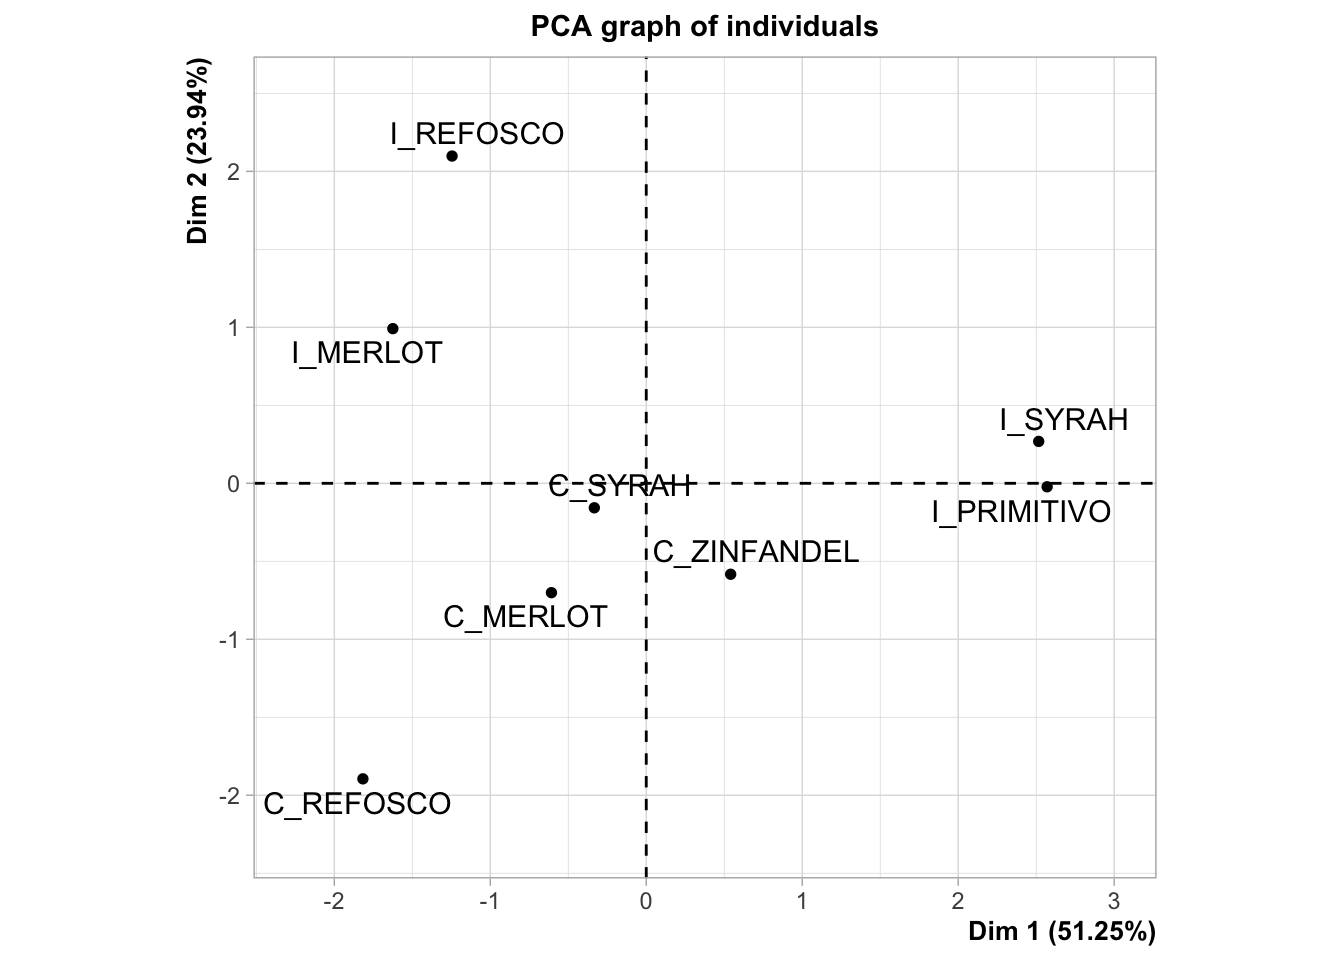
\includegraphics[keepaspectratio]{06-PCA_files/figure-latex/unnamed-chunk-16-2.pdf}} \pandocbounded{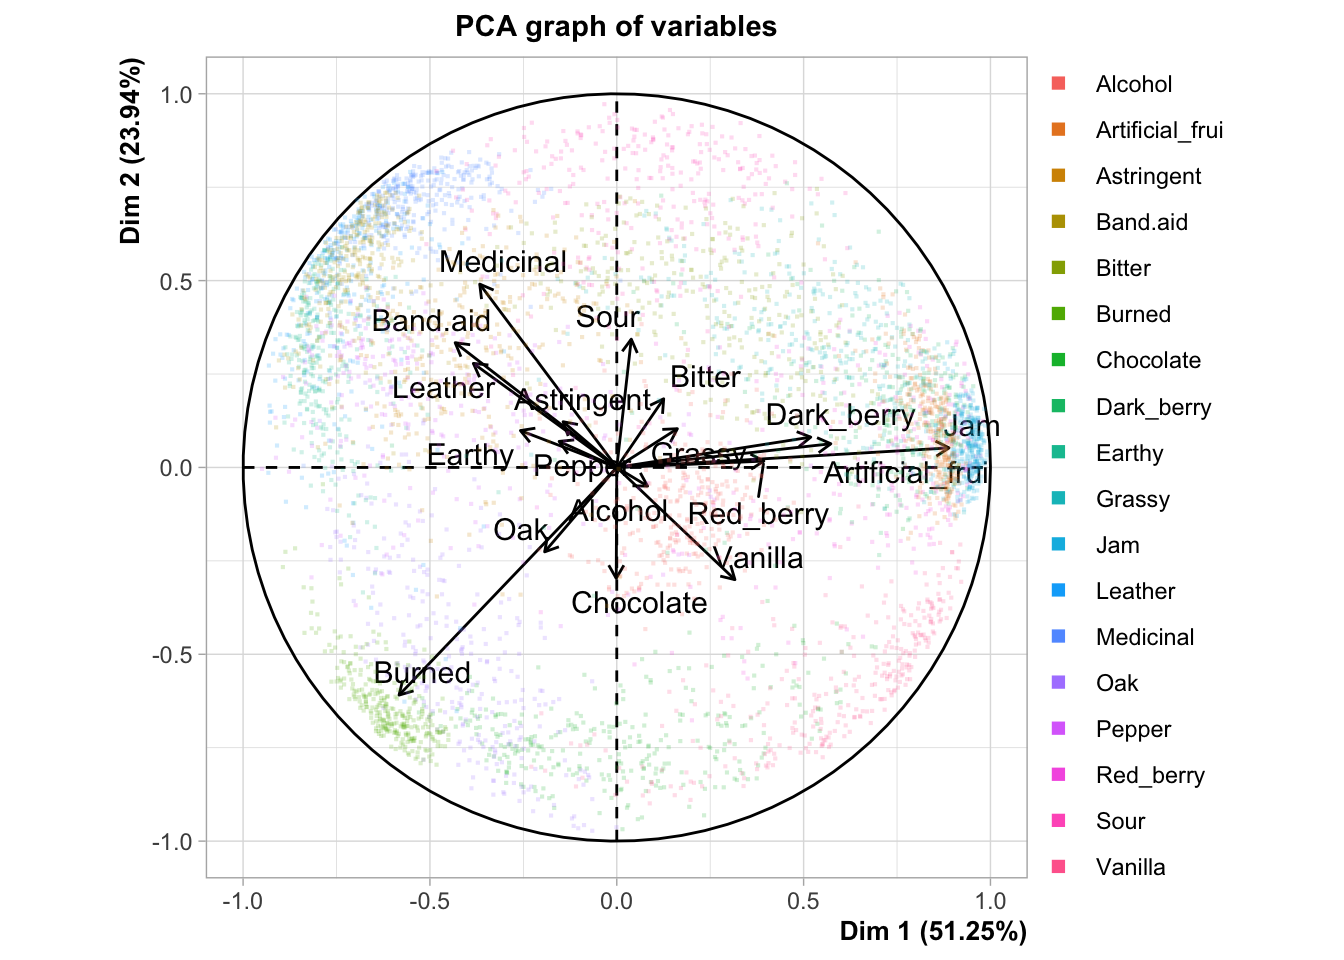
\includegraphics[keepaspectratio]{06-PCA_files/figure-latex/unnamed-chunk-16-3.pdf}} \pandocbounded{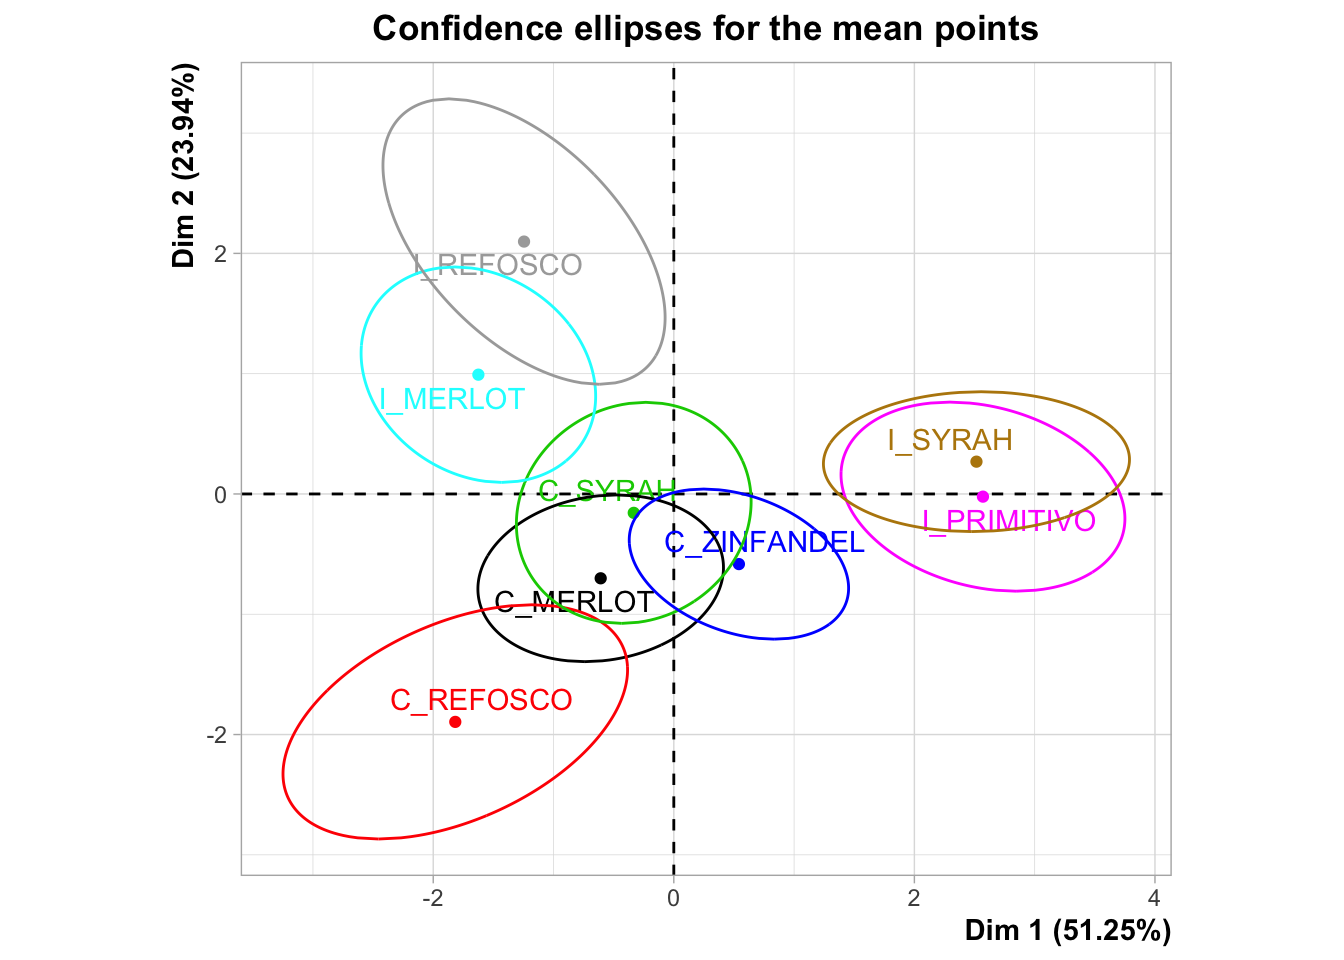
\includegraphics[keepaspectratio]{06-PCA_files/figure-latex/unnamed-chunk-16-4.pdf}}

I'm not a huge fan of \texttt{panellipse()} because it's pretty opaque. I can't find the documentation on what it's doing, and there doesn't seem to be an associated journal article. It doesn't really document how it is resampling or give easily understood descriptions of what the results (both numerical and graphical) it is producing \emph{mean}. Here is the plot that HGH uses for the original \textbf{R Opus}:

\begin{Shaded}
\begin{Highlighting}[]
\NormalTok{panellipse\_res}\SpecialCharTok{$}\NormalTok{graph}\SpecialCharTok{$}\NormalTok{plotIndEll}
\end{Highlighting}
\end{Shaded}

\pandocbounded{\includegraphics[keepaspectratio]{06-PCA_files/figure-latex/unnamed-chunk-17-1.pdf}}

The confidence ellipses are definitely being drawn around 95\% of the resampled results from the bootstrapping procedure, but I'm not sure if this is a bootstrap based on, for example, the ``partial bootstrap'' or the ``truncated bootstrap''. We will us a naive approach to producing a partial bootstrap in order to do some resampling and compare it.

It is also worth noting that the plot produced here is different than that produced in the original \textbf{R Opus}, so either there is simulation variability (probably) or the underlying program has changed between 2015 and now (also possible). The overall conclusions are not greatly different but the overlapping areas can vary quite dramatically.

The basic approach (which we saw back in the CVA section of the \textbf{R Opus}) is to draw a new set of bootstrapped observations for each product: we need 42 observations per product to calculate a new mean. We then can use the projection function from our original PCA solution to project these results into our space; in a nod to the truncated bootstrap approach \citep{cadoretConstruction2013} we will use only the first 2 dimensions of the projection function to get the results so as not to overfit. Finally, we'll draw ellipses around our results to represent variability.

\begin{Shaded}
\begin{Highlighting}[]
\NormalTok{get\_bootstrapped\_pca\_means }\OtherTok{\textless{}{-}} \ControlFlowTok{function}\NormalTok{()\{}
  
\NormalTok{  descriptive\_data }\SpecialCharTok{\%\textgreater{}\%}
    \FunctionTok{select}\NormalTok{(}\SpecialCharTok{{-}}\NormalTok{NJ, }\SpecialCharTok{{-}}\NormalTok{NR) }\SpecialCharTok{\%\textgreater{}\%}
    \FunctionTok{group\_by}\NormalTok{(ProductName) }\SpecialCharTok{\%\textgreater{}\%}
    \CommentTok{\# Here we resample each wine {-} we draw 42 new observations for each wine}
    \CommentTok{\# with replacement}
    \FunctionTok{slice\_sample}\NormalTok{(}\AttributeTok{prop =} \DecValTok{1}\NormalTok{, }\AttributeTok{replace =} \ConstantTok{TRUE}\NormalTok{) }\SpecialCharTok{\%\textgreater{}\%}
    \CommentTok{\# We calculate the mean for the newly drawn samples}
    \FunctionTok{summarize\_if}\NormalTok{(is.numeric, }\SpecialCharTok{\textasciitilde{}}\FunctionTok{mean}\NormalTok{(.)) }\SpecialCharTok{\%\textgreater{}\%}
    \CommentTok{\# And then we center the means (by subtracting the column means)}
    \FunctionTok{mutate\_if}\NormalTok{(is.numeric, }\SpecialCharTok{\textasciitilde{}}\NormalTok{. }\SpecialCharTok{{-}} \FunctionTok{mean}\NormalTok{(.)) }\SpecialCharTok{\%\textgreater{}\%}
    \FunctionTok{nest}\NormalTok{(}\AttributeTok{data =} \SpecialCharTok{{-}}\NormalTok{ProductName) }\SpecialCharTok{\%\textgreater{}\%}
    \FunctionTok{mutate}\NormalTok{(}\AttributeTok{means =} \FunctionTok{map}\NormalTok{(data, }\SpecialCharTok{\textasciitilde{}}\FunctionTok{as.matrix}\NormalTok{(.x)),}
           \AttributeTok{pc1 =} \FunctionTok{map\_dbl}\NormalTok{(means, }\SpecialCharTok{\textasciitilde{}}\NormalTok{ .x }\SpecialCharTok{\%*\%}\NormalTok{ means\_pca}\SpecialCharTok{$}\NormalTok{svd}\SpecialCharTok{$}\NormalTok{V[, }\DecValTok{1}\NormalTok{]),}
           \AttributeTok{pc2 =} \FunctionTok{map\_dbl}\NormalTok{(means, }\SpecialCharTok{\textasciitilde{}}\NormalTok{ .x }\SpecialCharTok{\%*\%}\NormalTok{ means\_pca}\SpecialCharTok{$}\NormalTok{svd}\SpecialCharTok{$}\NormalTok{V[, }\DecValTok{2}\NormalTok{])) }\SpecialCharTok{\%\textgreater{}\%}
    \FunctionTok{select}\NormalTok{(}\SpecialCharTok{{-}}\NormalTok{data, }\SpecialCharTok{{-}}\NormalTok{means)}
  
\NormalTok{\}}

\CommentTok{\# Make it reproducible}
\FunctionTok{set.seed}\NormalTok{(}\DecValTok{6}\NormalTok{)}

\NormalTok{pca\_boots }\OtherTok{\textless{}{-}} 
  \FunctionTok{tibble}\NormalTok{(}\AttributeTok{boot\_id =} \DecValTok{1}\SpecialCharTok{:}\DecValTok{100}\NormalTok{) }\SpecialCharTok{\%\textgreater{}\%}
  \FunctionTok{mutate}\NormalTok{(}\AttributeTok{bootstrapped\_data =} \FunctionTok{map}\NormalTok{(boot\_id, }\SpecialCharTok{\textasciitilde{}}\FunctionTok{get\_bootstrapped\_pca\_means}\NormalTok{())) }\SpecialCharTok{\%\textgreater{}\%}
  \FunctionTok{unnest}\NormalTok{(bootstrapped\_data)}

\NormalTok{p\_scores }\SpecialCharTok{+}
  \FunctionTok{geom\_point}\NormalTok{(}\AttributeTok{data =}\NormalTok{ pca\_boots, }
             \AttributeTok{inherit.aes =} \ConstantTok{FALSE}\NormalTok{,}
             \FunctionTok{aes}\NormalTok{(}\AttributeTok{x =}\NormalTok{ pc1, }\AttributeTok{y =}\NormalTok{ pc2, }\AttributeTok{color =}\NormalTok{ ProductName), }
             \AttributeTok{alpha =} \DecValTok{1}\SpecialCharTok{/}\DecValTok{2}\NormalTok{, }\AttributeTok{size =} \DecValTok{1}\SpecialCharTok{/}\DecValTok{2}\NormalTok{) }\SpecialCharTok{+}
  \FunctionTok{stat\_ellipse}\NormalTok{(}\AttributeTok{data =}\NormalTok{ pca\_boots, }\AttributeTok{inherit.aes =} \ConstantTok{FALSE}\NormalTok{,}
               \FunctionTok{aes}\NormalTok{(}\AttributeTok{x =}\NormalTok{ pc1, }\AttributeTok{y =}\NormalTok{ pc2, }\AttributeTok{color =}\NormalTok{ ProductName))}
\end{Highlighting}
\end{Shaded}

\pandocbounded{\includegraphics[keepaspectratio]{06-PCA_files/figure-latex/unnamed-chunk-18-1.pdf}}

Our results are pretty close, but not exactly the same. It seems like our method of generating bootstrapped scores (via resampling followed by projection via the \(\mathbf Q\) matrix from SVD) is potentially more liberal in product separation than that from the \texttt{panellipse()} function. Perhaps \texttt{panellipse()} is using the ``truncated bootstrap'' approach \citep{cadoretConstruction2013}, which solves a full PCA with the resampled data, then aligns it with the original observed space via \hyperref[generalized-procrustes-analysis]{Generalized Procrustes Analysis}, then repeats that process a large number (e.g., 1000) times..

\section{Comparison of products with PCA}\label{comparison-of-products-with-pca}

HGH then used the \texttt{panellipse()} results to get Hotelling's \(T^2\) stats for each set of products. I believe that Hotelling's \(T^2\) is a generalization of the \(t\)-distribution to multivariate data. These were accessed from the outputs of \texttt{panellipse()}, which we stored in \texttt{panellipse\_res}.

\begin{Shaded}
\begin{Highlighting}[]
\FunctionTok{names}\NormalTok{(panellipse\_res)}
\end{Highlighting}
\end{Shaded}

\begin{verbatim}
## [1] "eig"         "coordinates" "hotelling"   "graph"       "correl"
\end{verbatim}

The \texttt{SensoMineR::coltable()} function HGH used is a visualization function for this kind of output, let's take a look.

\begin{Shaded}
\begin{Highlighting}[]
\NormalTok{SensoMineR}\SpecialCharTok{::}\FunctionTok{coltable}\NormalTok{(panellipse\_res}\SpecialCharTok{$}\NormalTok{hotelling, }\AttributeTok{main.title =} \StringTok{"Hotelling\textquotesingle{}s T2 for all products"}\NormalTok{)}
\end{Highlighting}
\end{Shaded}

\pandocbounded{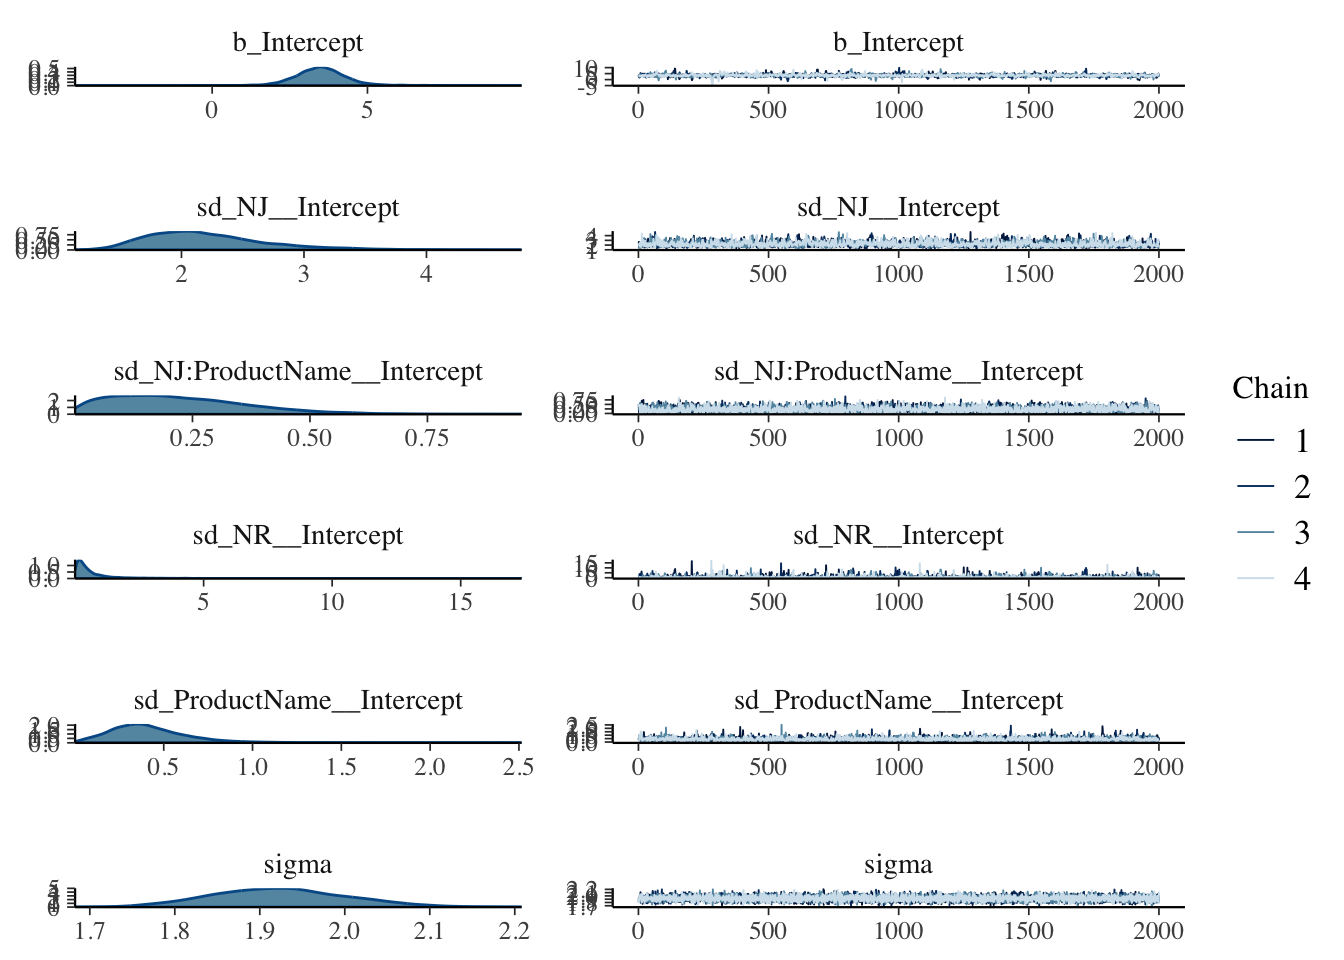
\includegraphics[keepaspectratio]{06-PCA_files/figure-latex/unnamed-chunk-20-1.pdf}}

Let's practice how to make a similar table from this kind of data. The actual \texttt{panellipse\_res\$hotelling} object is just a square matrix. We can use this as input for something like the \texttt{geom\_tile()} function with the right kind of wrangling.

\begin{Shaded}
\begin{Highlighting}[]
\CommentTok{\# First wrangle}

\NormalTok{panellipse\_res}\SpecialCharTok{$}\NormalTok{hotelling }\SpecialCharTok{\%\textgreater{}\%}
  \FunctionTok{as\_tibble}\NormalTok{(}\AttributeTok{rownames =} \StringTok{"x"}\NormalTok{) }\SpecialCharTok{\%\textgreater{}\%}
  \FunctionTok{pivot\_longer}\NormalTok{(}\SpecialCharTok{{-}}\NormalTok{x, }\AttributeTok{names\_to =} \StringTok{"y"}\NormalTok{) }\SpecialCharTok{\%\textgreater{}\%}
  \FunctionTok{mutate}\NormalTok{(}\AttributeTok{color =} \FunctionTok{if\_else}\NormalTok{(value }\SpecialCharTok{\textless{}} \FloatTok{0.05}\NormalTok{, }\StringTok{"pink"}\NormalTok{, }\StringTok{"white"}\NormalTok{)) }\SpecialCharTok{\%\textgreater{}\%}
  
  \CommentTok{\# Now plot}
  
  \FunctionTok{ggplot}\NormalTok{(}\FunctionTok{aes}\NormalTok{(}\AttributeTok{x =}\NormalTok{ x, }\AttributeTok{y =}\NormalTok{ y)) }\SpecialCharTok{+}
  \FunctionTok{geom\_tile}\NormalTok{(}\FunctionTok{aes}\NormalTok{(}\AttributeTok{fill =}\NormalTok{ color),}
            \AttributeTok{color =} \StringTok{"black"}\NormalTok{) }\SpecialCharTok{+}
  \FunctionTok{geom\_text}\NormalTok{(}\FunctionTok{aes}\NormalTok{(}\AttributeTok{label =} \FunctionTok{round}\NormalTok{(value, }\DecValTok{2}\NormalTok{))) }\SpecialCharTok{+}
  \FunctionTok{scale\_fill\_manual}\NormalTok{(}\AttributeTok{values =} \FunctionTok{c}\NormalTok{(}\StringTok{"pink"}\NormalTok{, }\StringTok{"white"}\NormalTok{)) }\SpecialCharTok{+} 
  \FunctionTok{coord\_fixed}\NormalTok{() }\SpecialCharTok{+} 
  
  \CommentTok{\# Everything after this is just making the plot look nice}
  
  \FunctionTok{scale\_x\_discrete}\NormalTok{(}\AttributeTok{position =} \StringTok{"top"}\NormalTok{) }\SpecialCharTok{+} 
  \FunctionTok{scale\_y\_discrete}\NormalTok{(}\AttributeTok{limits =}\NormalTok{ rev) }\SpecialCharTok{+} 
  \FunctionTok{labs}\NormalTok{(}\AttributeTok{x =} \ConstantTok{NULL}\NormalTok{, }
       \AttributeTok{y =} \ConstantTok{NULL}\NormalTok{,}
       \AttributeTok{title =} \FunctionTok{bquote}\NormalTok{(}\StringTok{"Pairwise Hotelling\textquotesingle{}s"}\SpecialCharTok{\textasciitilde{}}\FunctionTok{italic}\NormalTok{(T)}\SpecialCharTok{\^{}}\DecValTok{2}\NormalTok{),}
       \AttributeTok{subtitle =} \FunctionTok{bquote}\NormalTok{(}\FunctionTok{italic}\NormalTok{(p)}\SpecialCharTok{*}\StringTok{"{-}values"}\SpecialCharTok{\textless{}}\FloatTok{0.05}\SpecialCharTok{\textasciitilde{}}\StringTok{"are highlighted in pink"}\NormalTok{)) }\SpecialCharTok{+} 
  \FunctionTok{theme\_minimal}\NormalTok{() }\SpecialCharTok{+} 
  \FunctionTok{theme}\NormalTok{(}\AttributeTok{axis.text.x =} \FunctionTok{element\_text}\NormalTok{(}\AttributeTok{angle =} \DecValTok{270}\NormalTok{, }\AttributeTok{hjust =} \DecValTok{1}\NormalTok{),}
        \AttributeTok{legend.position =} \StringTok{"none"}\NormalTok{,}
        \AttributeTok{axis.ticks =} \FunctionTok{element\_blank}\NormalTok{(),}
        \AttributeTok{panel.grid =} \FunctionTok{element\_blank}\NormalTok{())}
\end{Highlighting}
\end{Shaded}

\pandocbounded{\includegraphics[keepaspectratio]{06-PCA_files/figure-latex/unnamed-chunk-21-1.pdf}}

Notice the \texttt{ggplot2} syntax above is kind of complicated, but that's because I did it all at once, and I wanted to do a lot of minor things like remove axis ticks, so as to replicate the plot from the \texttt{panellipse()} function closely.

As a bonus, we will quickly look into how to conduct Hotelling's \(T^2\) tests ourselves, and then leave the world of PCA (for now) to turn to methods for cluster analysis.

\begin{Shaded}
\begin{Highlighting}[]
\CommentTok{\# We need pairs of products {-} if we wanted to make all pairwise comparisons it}
\CommentTok{\# would be possible to do so using, for example, nested \textasciigrave{}for()\textasciigrave{} loops or some}
\CommentTok{\# kind of list{-}table structure}
\NormalTok{hotelling\_demo\_data }\OtherTok{\textless{}{-}} 
\NormalTok{  descriptive\_data }\SpecialCharTok{\%\textgreater{}\%}
  \FunctionTok{filter}\NormalTok{(ProductName }\SpecialCharTok{\%in\%} \FunctionTok{c}\NormalTok{(}\StringTok{"C\_MERLOT"}\NormalTok{, }\StringTok{"C\_REFOSCO"}\NormalTok{)) }\SpecialCharTok{\%\textgreater{}\%}
  \FunctionTok{select}\NormalTok{(}\SpecialCharTok{{-}}\NormalTok{NJ, }\SpecialCharTok{{-}}\NormalTok{NR)}

\NormalTok{DescTools}\SpecialCharTok{::}\FunctionTok{HotellingsT2Test}\NormalTok{(}\AttributeTok{formula =} \FunctionTok{as.matrix}\NormalTok{(hotelling\_demo\_data[, }\SpecialCharTok{{-}}\DecValTok{1}\NormalTok{]) }\SpecialCharTok{\textasciitilde{}}\NormalTok{ ProductName,}
                            \AttributeTok{data =}\NormalTok{ hotelling\_demo\_data)}
\end{Highlighting}
\end{Shaded}

\begin{verbatim}
## 
##  Hotelling's two sample T2-test
## 
## data:  as.matrix(hotelling_demo_data[, -1]) by ProductName
## T.2 = 2.4053, df1 = 20, df2 = 63, p-value = 0.004345
## alternative hypothesis: true location difference is not equal to c(0,0,0,0,0,0,0,0,0,0,0,0,0,0,0,0,0,0,0,0)
\end{verbatim}

These results are not the same as those given in the \texttt{panellipse()} output; I suspect after reading \texttt{?panellipse} that this is because internally that function is running a Hotelling's \(T^2\) test on the PCA results, rather than on the raw data, but I am not sure and I am not willing to try to interpret the under-the-hood code. If you know, please reach out and let me know!

In general, it seems like using something like CVA and investigating the separability of means there instead of using pairwise Hotelling's \(T^2\) tests would be safer in terms of familywise error inflation.

\section{Packages used in this chapter}\label{packages-used-in-this-chapter-5}

\begin{Shaded}
\begin{Highlighting}[]
\FunctionTok{sessionInfo}\NormalTok{()}
\end{Highlighting}
\end{Shaded}

\begin{verbatim}
## R version 4.4.1 (2024-06-14)
## Platform: x86_64-apple-darwin20
## Running under: macOS 15.2
## 
## Matrix products: default
## BLAS:   /Library/Frameworks/R.framework/Versions/4.4-x86_64/Resources/lib/libRblas.0.dylib 
## LAPACK: /Library/Frameworks/R.framework/Versions/4.4-x86_64/Resources/lib/libRlapack.dylib;  LAPACK version 3.12.0
## 
## locale:
## [1] en_US.UTF-8/en_US.UTF-8/en_US.UTF-8/C/en_US.UTF-8/en_US.UTF-8
## 
## time zone: America/New_York
## tzcode source: internal
## 
## attached base packages:
## [1] stats     graphics  grDevices datasets  utils     methods   base     
## 
## other attached packages:
##  [1] patchwork_1.2.0 here_1.0.1      FactoMineR_2.11 lubridate_1.9.3
##  [5] forcats_1.0.0   stringr_1.5.1   dplyr_1.1.4     purrr_1.0.2    
##  [9] readr_2.1.5     tidyr_1.3.1     tibble_3.2.1    ggplot2_3.5.1  
## [13] tidyverse_2.0.0
## 
## loaded via a namespace (and not attached):
##  [1] Exact_3.3            tidyselect_1.2.1     rootSolve_1.8.2.4   
##  [4] farver_2.1.2         fastmap_1.2.0        janeaustenr_1.0.0   
##  [7] digest_0.6.37        timechange_0.3.0     estimability_1.5.1  
## [10] lifecycle_1.0.4      cluster_2.1.6        multcompView_0.1-10 
## [13] tokenizers_0.3.0     lmom_3.2             magrittr_2.0.3      
## [16] compiler_4.4.1       rlang_1.1.4          tools_4.4.1         
## [19] utf8_1.2.4           yaml_2.3.8           tidytext_0.4.2      
## [22] data.table_1.15.4    knitr_1.46           labeling_0.4.3      
## [25] htmlwidgets_1.6.4    bit_4.0.5            scatterplot3d_0.3-44
## [28] plyr_1.8.9           KernSmooth_2.23-26   expm_1.0-0          
## [31] withr_3.0.0          grid_4.4.1           fansi_1.0.6         
## [34] SensoMineR_1.27      AlgDesign_1.2.1      xtable_1.8-4        
## [37] e1071_1.7-16         colorspace_2.1-0     emmeans_1.10.2      
## [40] scales_1.3.0         gtools_3.9.5         MASS_7.3-60.2       
## [43] flashClust_1.01-2    cli_3.6.3            mvtnorm_1.2-5       
## [46] rmarkdown_2.27       crayon_1.5.2         generics_0.1.3      
## [49] rstudioapi_0.16.0    httr_1.4.7           reshape2_1.4.4      
## [52] tzdb_0.4.0           readxl_1.4.3         gld_2.6.6           
## [55] proxy_0.4-27         parallel_4.4.1       cellranger_1.1.0    
## [58] vctrs_0.6.5          boot_1.3-30          Matrix_1.7-0        
## [61] bookdown_0.39        hms_1.1.3            bit64_4.0.5         
## [64] ggrepel_0.9.5        glue_1.7.0           DT_0.33             
## [67] stringi_1.8.4        gtable_0.3.5         munsell_0.5.1       
## [70] pillar_1.9.0         htmltools_0.5.8.1    R6_2.5.1            
## [73] rprojroot_2.0.4      vroom_1.6.5          evaluate_0.23       
## [76] lattice_0.22-6       haven_2.5.4          highr_0.10          
## [79] SnowballC_0.7.1      leaps_3.1            renv_1.0.9          
## [82] class_7.3-22         DescTools_0.99.58    Rcpp_1.0.13         
## [85] coda_0.19-4.1        xfun_0.49            pkgconfig_2.0.3
\end{verbatim}

\chapter{Cluster analysis}\label{cluster-analysis}

The goal of any cluster analysis is to find groups (``clusters'') of observations that are ``close to'' each other in some sense, so as to reveal underlying structure in the data: typically, we would want to know that groups of more than one observation are very ``close'' so that we can speak about the group instead of the original observations. In most sensory evaluation, ``close'' is usually taken to mean ``similar'', as the definitions of ``close'' we will operationalize are based on the sensory descriptors, so that observations that are ``close'' to each other will, in some sense, have similar sensory profiles.

We could also use cluster analysis to explore possible hypotheses, if we have some hypotheses about the underlying group structure that exists--for example, if we think that wines made from the same grape would be more similar to each other, we'd expect those wines to show up in the same group. We'll explore this more as we look at our results.

We start by loading our results, as before. We will also define a tibble of product means, which will be our main data input to start with.

\begin{Shaded}
\begin{Highlighting}[]
\FunctionTok{library}\NormalTok{(tidyverse)}
\FunctionTok{library}\NormalTok{(here)}
\FunctionTok{library}\NormalTok{(factoextra) }\CommentTok{\# this is new}

\CommentTok{\# I\textquotesingle{}ve decided to use the \textasciigrave{}across()\textasciigrave{} syntax instead of the scoped mutate\_*()}
\CommentTok{\# functions, for documentation check out ?across()}
\NormalTok{descriptive\_data }\OtherTok{\textless{}{-}} \FunctionTok{read\_csv}\NormalTok{(}\FunctionTok{here}\NormalTok{(}\StringTok{"data/torriDAFinal.csv"}\NormalTok{)) }\SpecialCharTok{\%\textgreater{}\%}
  \FunctionTok{mutate}\NormalTok{(}\FunctionTok{across}\NormalTok{(}\DecValTok{1}\SpecialCharTok{:}\DecValTok{3}\NormalTok{, }\SpecialCharTok{\textasciitilde{}}\FunctionTok{as.factor}\NormalTok{(.)))}

\NormalTok{descriptive\_means }\OtherTok{\textless{}{-}} 
\NormalTok{  descriptive\_data }\SpecialCharTok{\%\textgreater{}\%}
  \FunctionTok{group\_by}\NormalTok{(ProductName) }\SpecialCharTok{\%\textgreater{}\%}
  \FunctionTok{summarize}\NormalTok{(}\FunctionTok{across}\NormalTok{(}\FunctionTok{where}\NormalTok{(is.numeric), }\SpecialCharTok{\textasciitilde{}}\FunctionTok{mean}\NormalTok{(.)))}
\end{Highlighting}
\end{Shaded}

We're going to mostly use the built in \texttt{stats::hclust()} function for most of this workflow, but do know that this is the simplest (and perhaps not best) clustering tool available in \texttt{R}. It will do for our purposes.

In the \textbf{R Opus}, HGH \emph{scales} the mean data to have zero-means and unit-variance. This choice (it is not necessary for calculation) means that all descriptors will have equal impact on our estimates of proximity for the purpose of clustering. We'll follow along.

\begin{Shaded}
\begin{Highlighting}[]
\NormalTok{descriptive\_means\_scaled }\OtherTok{\textless{}{-}} 
\NormalTok{  descriptive\_means }\SpecialCharTok{\%\textgreater{}\%}
  \CommentTok{\# This line is dense {-} notice the "lambda" ("\textasciitilde{}") function that uses multiple}
  \CommentTok{\# references to the same column: we are subtracting the column mean and}
  \CommentTok{\# dividing by the column sd for each column.}
  \FunctionTok{mutate}\NormalTok{(}\FunctionTok{across}\NormalTok{(}\FunctionTok{where}\NormalTok{(is.numeric), }\SpecialCharTok{\textasciitilde{}}\NormalTok{ (. }\SpecialCharTok{{-}} \FunctionTok{mean}\NormalTok{(.)) }\SpecialCharTok{/} \FunctionTok{sd}\NormalTok{(.)))}
\end{Highlighting}
\end{Shaded}

Now we're ready to think about ``close''. As the word implies, we're going to examine the distances among all of our products. The built in function in \texttt{R} to calculate distance is \texttt{stats::dist()}. This will serve our purposes well.

\begin{Shaded}
\begin{Highlighting}[]
\NormalTok{descriptive\_distance }\OtherTok{\textless{}{-}} 
\NormalTok{  descriptive\_means\_scaled }\SpecialCharTok{\%\textgreater{}\%}
  \CommentTok{\# We need to remember to move our variable column to the "rownames" attribute}
  \CommentTok{\# so that the older function keeps it (and doesn\textquotesingle{}t try to find distances}
  \CommentTok{\# between character vectors)}
  \FunctionTok{column\_to\_rownames}\NormalTok{(}\StringTok{"ProductName"}\NormalTok{) }\SpecialCharTok{\%\textgreater{}\%}
  \FunctionTok{dist}\NormalTok{(}\AttributeTok{method =} \StringTok{"euclidean"}\NormalTok{)}

\NormalTok{descriptive\_distance}
\end{Highlighting}
\end{Shaded}

\begin{verbatim}
##             C_MERLOT C_REFOSCO  C_SYRAH C_ZINFANDEL I_MERLOT I_PRIMITIVO
## C_REFOSCO   5.083950                                                    
## C_SYRAH     4.525147  5.472269                                          
## C_ZINFANDEL 3.909011  5.856348 4.817566                                 
## I_MERLOT    4.503404  6.405151 6.153529    6.522035                     
## I_PRIMITIVO 6.129930  7.853063 5.998705    5.543431 7.842528            
## I_REFOSCO   6.272963  6.992652 5.408757    6.917554 4.452965    8.514098
## I_SYRAH     6.911105  8.427799 6.359281    6.170264 7.546229    5.747512
##             I_REFOSCO
## C_REFOSCO            
## C_SYRAH              
## C_ZINFANDEL          
## I_MERLOT             
## I_PRIMITIVO          
## I_REFOSCO            
## I_SYRAH      7.537424
\end{verbatim}

The \texttt{dist()} function produces a lower-triangular matrix of the distances between each pair of mean vectors. Because we selected \texttt{method\ =\ "euclidean"} the distance is calculated as the typical (L2) norm: the square-root of the the sum of the squared differences between each attribute mean for the two products. Other common options are available, see \texttt{?dist}.

Technically, all (mathematical) distances must fulfill 4 properties:

\begin{enumerate}
\def\labelenumi{\arabic{enumi}.}
\tightlist
\item
  For any object, \(dist(a,a) = 0\) (the distance of an object to itself is always 0)
\item
  For all pairs of objects, \(dist(a,b) ≥ 0\) (all distances are positive or 0)
\item
  For any pair of objects, \(dist(a,b) = dist(b,a)\) (distance is symmetric)
\item
  For any three objects, \(dist(a,b) + dist(b,c) ≥ dist(a,c)\) (the triangle inequality - I like the \href{https://en.wikipedia.org/wiki/Distance\#Mathematical_formalization}{Wikipedia description} as ``intermediate objects can't speed you up'')
\end{enumerate}

Enough about distance! Let's get on with it. We can see that our distance matrix is all positive entries that give us some idea of ``how close'' each pair of objects is. Smaller numbers indicate proximity.

\section{Hierarchical clustering on distances}\label{hierarchical-clustering-on-distances}

One of the major families of clustering is called ``hierarchical'' clustering (HCA: Hierarchical Clustering Analysis). In plain language, hierarchical methods are iterative methods that start with the assumption that each object (sample) starts in its own group and then, for each step in the process, the two ``closest'' objects are merged into a group. Different strategies for calculating distance (between the merged groups, as we will typically stick with Euclidean distance as our base metric for singlets) and different methods for making the merge define the different hierarchical clustering approaches.

In the original \textbf{R Opus}, HGH demonstrates 4 different HCA methods. We'll look at each briefly.

\subsection{Ward's Method}\label{wards-method}

Ward's Method is probably the most commonly used (and intellectually satisfying approach). For Ward's method, to quote \citet[p.466]{rencherMethods2002}:

\begin{quote}
Ward's method, also called the incremental sum of squares method, uses the within cluster (squared) distances and the between-cluster (squared) distances\ldots{} Ward's method joins the two clusters A and B that minimize the increase in {[}the difference between the new AB cluster's within-distance and the old A and B within-distances{]}.
\end{quote}

Ward's method, qualitatively, tends to find balanced clusters that result from the merge of smaller clusters.

\begin{Shaded}
\begin{Highlighting}[]
\NormalTok{cluster\_ward }\OtherTok{\textless{}{-}}
\NormalTok{  descriptive\_distance }\SpecialCharTok{\%\textgreater{}\%}
  \FunctionTok{hclust}\NormalTok{(}\AttributeTok{method =} \StringTok{"ward.D2"}\NormalTok{)}
\end{Highlighting}
\end{Shaded}

Note that the original \textbf{R Opus} used \texttt{method\ =\ "ward"}--according to the documentation in \texttt{?hclust}:

\begin{quote}
Two different algorithms are found in the literature for Ward clustering. The one used by option ``ward.D'' (equivalent to the only Ward option ``ward'' in R versions ≤ 3.0.3) does not implement Ward's (1963) clustering criterion, whereas option ``ward.D2'' implements that criterion (Murtagh and Legendre 2014). With the latter, the dissimilarities are squared before cluster updating. Note that agnes(\emph{, method=``ward'') corresponds to hclust(}, ``ward.D2'').
\end{quote}

\begin{Shaded}
\begin{Highlighting}[]
\NormalTok{p\_ward }\OtherTok{\textless{}{-}} 
\NormalTok{  cluster\_ward }\SpecialCharTok{\%\textgreater{}\%}
  \FunctionTok{fviz\_dend}\NormalTok{(}\AttributeTok{k =} \DecValTok{3}\NormalTok{, }\AttributeTok{cex =} \DecValTok{2}\SpecialCharTok{/}\DecValTok{3}\NormalTok{)}
\end{Highlighting}
\end{Shaded}

We're going to use the \texttt{factoextra::fviz\_dend()} function for drawing our clusters. Long-story-short, the native \texttt{ggplot2} functions for plotting tree- and graph-like structures like ``dendrograms'' (the tree plots that are common for HCA results) don't really exist, and \texttt{fviz\_dend()} is going to do a lot of heavy lifting for us in the background by giving us a basic dendrogram \texttt{ggplot2} object that we can alter as we see fit using more familiar syntax.

\begin{Shaded}
\begin{Highlighting}[]
\NormalTok{p\_ward }\OtherTok{\textless{}{-}} 
\NormalTok{  p\_ward }\SpecialCharTok{+} 
  \CommentTok{\# Stretch out the y{-}axis so that we can see the labels}
  \FunctionTok{expand\_limits}\NormalTok{(}\AttributeTok{y =} \SpecialCharTok{{-}}\DecValTok{6}\NormalTok{) }\SpecialCharTok{+} 
  \CommentTok{\# Clean up the messiness}
  \FunctionTok{labs}\NormalTok{(}\AttributeTok{title =} \StringTok{"Clustering with Ward\textquotesingle{}s method"}\NormalTok{, }\AttributeTok{y =} \ConstantTok{NULL}\NormalTok{) }\SpecialCharTok{+}
  \FunctionTok{scale\_color\_viridis\_d}\NormalTok{() }\SpecialCharTok{+} 
  \FunctionTok{scale\_y\_continuous}\NormalTok{(}\AttributeTok{breaks =} \FunctionTok{c}\NormalTok{(}\DecValTok{0}\NormalTok{, }\DecValTok{5}\NormalTok{, }\DecValTok{10}\NormalTok{))}

\NormalTok{p\_ward}
\end{Highlighting}
\end{Shaded}

\pandocbounded{\includegraphics[keepaspectratio]{07-HCA_files/figure-latex/unnamed-chunk-6-1.pdf}}

Notice that we had to \emph{tell} the program (in this case \texttt{fviz\_dend()}) how many groups we wanted to label separately (\texttt{k\ =\ 3}). We're following HGH here. In general, while there are methods for attempting to determine the ``right'' number of groups from HCA, this involves ``researcher degrees of freedom'' (i.e., ``good judgment'').

\subsection{Single linkage}\label{single-linkage}

Single linkage is also called ``nearest neighbor'' clustering. In single-linkage, the key element is that the distance between any two \emph{clusters} \(A\) and \(B\) is defined as the \emph{minimum} distance between a point \(a\) in \(A\) and a point \(b\) in \(B\). Single linkage is, therefore, ``greedy'', because big clusters will tend to get bigger: there is a greater chance that a large cluster will have a small distance between \emph{some} point within it and another point outside it.

\begin{Shaded}
\begin{Highlighting}[]
\NormalTok{cluster\_single }\OtherTok{\textless{}{-}} 
\NormalTok{  descriptive\_distance }\SpecialCharTok{\%\textgreater{}\%}
  \FunctionTok{hclust}\NormalTok{(}\AttributeTok{method =} \StringTok{"single"}\NormalTok{)}
\end{Highlighting}
\end{Shaded}

We can use the same number of groups (\texttt{k\ =\ 3}) so we can have a consistent comparison among the methods.

\begin{Shaded}
\begin{Highlighting}[]
\NormalTok{p\_single }\OtherTok{\textless{}{-}} 
\NormalTok{  cluster\_single }\SpecialCharTok{\%\textgreater{}\%}
  \FunctionTok{fviz\_dend}\NormalTok{(}\AttributeTok{k =} \DecValTok{3}\NormalTok{, }\AttributeTok{cex =} \DecValTok{2}\SpecialCharTok{/}\DecValTok{3}\NormalTok{) }\SpecialCharTok{+} 
  \FunctionTok{expand\_limits}\NormalTok{(}\AttributeTok{y =} \SpecialCharTok{{-}}\DecValTok{3}\NormalTok{) }\SpecialCharTok{+} 
  \FunctionTok{scale\_color\_viridis\_d}\NormalTok{() }\SpecialCharTok{+}
  \FunctionTok{labs}\NormalTok{(}\AttributeTok{y =} \ConstantTok{NULL}\NormalTok{, }\AttributeTok{title =} \StringTok{"Clustering with Single Linkage"}\NormalTok{) }\SpecialCharTok{+} 
  \FunctionTok{scale\_y\_continuous}\NormalTok{(}\AttributeTok{breaks =} \FunctionTok{c}\NormalTok{(}\DecValTok{0}\NormalTok{, }\DecValTok{5}\NormalTok{, }\DecValTok{10}\NormalTok{))}

\NormalTok{p\_single}
\end{Highlighting}
\end{Shaded}

\pandocbounded{\includegraphics[keepaspectratio]{07-HCA_files/figure-latex/unnamed-chunk-8-1.pdf}}

Notice the ``greediness'': large single group keeps adding a single new observation at each step of the algorithm, resulting in this characteristic ``step'' pattern. For most situations, single linkage is a not a recommended approach for clustering.

\subsection{Complete Linkage}\label{complete-linkage}

The complete linkage approach is just the opposite of the single linkage method: the distance between two clusters is the \emph{maximum} distance between all two points \(a\) and \(b\) in clusters \(A\) and \(B\), respectively. With this definition, the same iterative approach is carried out and the two closest clusters are merged at each step.

\begin{Shaded}
\begin{Highlighting}[]
\NormalTok{cluster\_complete }\OtherTok{\textless{}{-}} 
\NormalTok{  descriptive\_distance }\SpecialCharTok{\%\textgreater{}\%}
  \FunctionTok{hclust}\NormalTok{(}\AttributeTok{method =} \StringTok{"complete"}\NormalTok{)}

\NormalTok{p\_complete }\OtherTok{\textless{}{-}}
\NormalTok{  cluster\_complete }\SpecialCharTok{\%\textgreater{}\%}
  \FunctionTok{fviz\_dend}\NormalTok{(}\AttributeTok{k =} \DecValTok{3}\NormalTok{, }\AttributeTok{cex =} \DecValTok{2}\SpecialCharTok{/}\DecValTok{3}\NormalTok{) }\SpecialCharTok{+} 
  \FunctionTok{expand\_limits}\NormalTok{(}\AttributeTok{y =} \SpecialCharTok{{-}}\DecValTok{3}\NormalTok{) }\SpecialCharTok{+} 
  \FunctionTok{labs}\NormalTok{(}\AttributeTok{y =} \ConstantTok{NULL}\NormalTok{, }\AttributeTok{title =} \StringTok{"Clustering with Complete Linkage"}\NormalTok{) }\SpecialCharTok{+}
  \FunctionTok{scale\_color\_viridis\_d}\NormalTok{() }\SpecialCharTok{+}
  \FunctionTok{scale\_y\_continuous}\NormalTok{(}\AttributeTok{breaks =} \FunctionTok{c}\NormalTok{(}\DecValTok{0}\NormalTok{, }\DecValTok{5}\NormalTok{, }\DecValTok{10}\NormalTok{))}

\NormalTok{p\_complete}
\end{Highlighting}
\end{Shaded}

\pandocbounded{\includegraphics[keepaspectratio]{07-HCA_files/figure-latex/unnamed-chunk-9-1.pdf}}

Intuitively, complete linkage avoids the ``greediness'' problem of single linkage. It is the default method used in \texttt{hclust()}: see \texttt{?hclust}.

\subsection{Average Linkage}\label{average-linkage}

As the name implies, in the average linkage method, the distance between two clusters is defined as the average distance between all objects \(a_i\) in \(A\) and all objects \(b_j\) in \(B\).

\begin{Shaded}
\begin{Highlighting}[]
\NormalTok{cluster\_average }\OtherTok{\textless{}{-}}
\NormalTok{  descriptive\_distance }\SpecialCharTok{\%\textgreater{}\%}
  \FunctionTok{hclust}\NormalTok{(}\AttributeTok{method =} \StringTok{"average"}\NormalTok{)}

\NormalTok{p\_average }\OtherTok{\textless{}{-}} 
\NormalTok{  cluster\_average }\SpecialCharTok{\%\textgreater{}\%}
  \FunctionTok{fviz\_dend}\NormalTok{(}\AttributeTok{k =} \DecValTok{3}\NormalTok{, }\AttributeTok{cex =} \DecValTok{2}\SpecialCharTok{/}\DecValTok{3}\NormalTok{) }\SpecialCharTok{+}
  \FunctionTok{expand\_limits}\NormalTok{(}\AttributeTok{y =} \SpecialCharTok{{-}}\DecValTok{3}\NormalTok{) }\SpecialCharTok{+} 
  \FunctionTok{labs}\NormalTok{(}\AttributeTok{title =} \StringTok{"Clustering with Average Linkage"}\NormalTok{, }\AttributeTok{y =} \ConstantTok{NULL}\NormalTok{) }\SpecialCharTok{+} 
  \FunctionTok{scale\_color\_viridis\_d}\NormalTok{() }\SpecialCharTok{+} 
  \FunctionTok{scale\_y\_continuous}\NormalTok{(}\AttributeTok{breaks =} \FunctionTok{c}\NormalTok{(}\DecValTok{0}\NormalTok{, }\DecValTok{5}\NormalTok{, }\DecValTok{10}\NormalTok{))}

\NormalTok{p\_average}
\end{Highlighting}
\end{Shaded}

\pandocbounded{\includegraphics[keepaspectratio]{07-HCA_files/figure-latex/unnamed-chunk-10-1.pdf}}

\subsection{Comparing methods}\label{comparing-methods}

Let's look at the results of our cluster analyses side by side.

\begin{Shaded}
\begin{Highlighting}[]
\FunctionTok{library}\NormalTok{(patchwork)}

\NormalTok{(p\_ward }\SpecialCharTok{+}\NormalTok{ p\_single) }\SpecialCharTok{/}\NormalTok{ (p\_complete }\SpecialCharTok{+}\NormalTok{ p\_average)}
\end{Highlighting}
\end{Shaded}

\pandocbounded{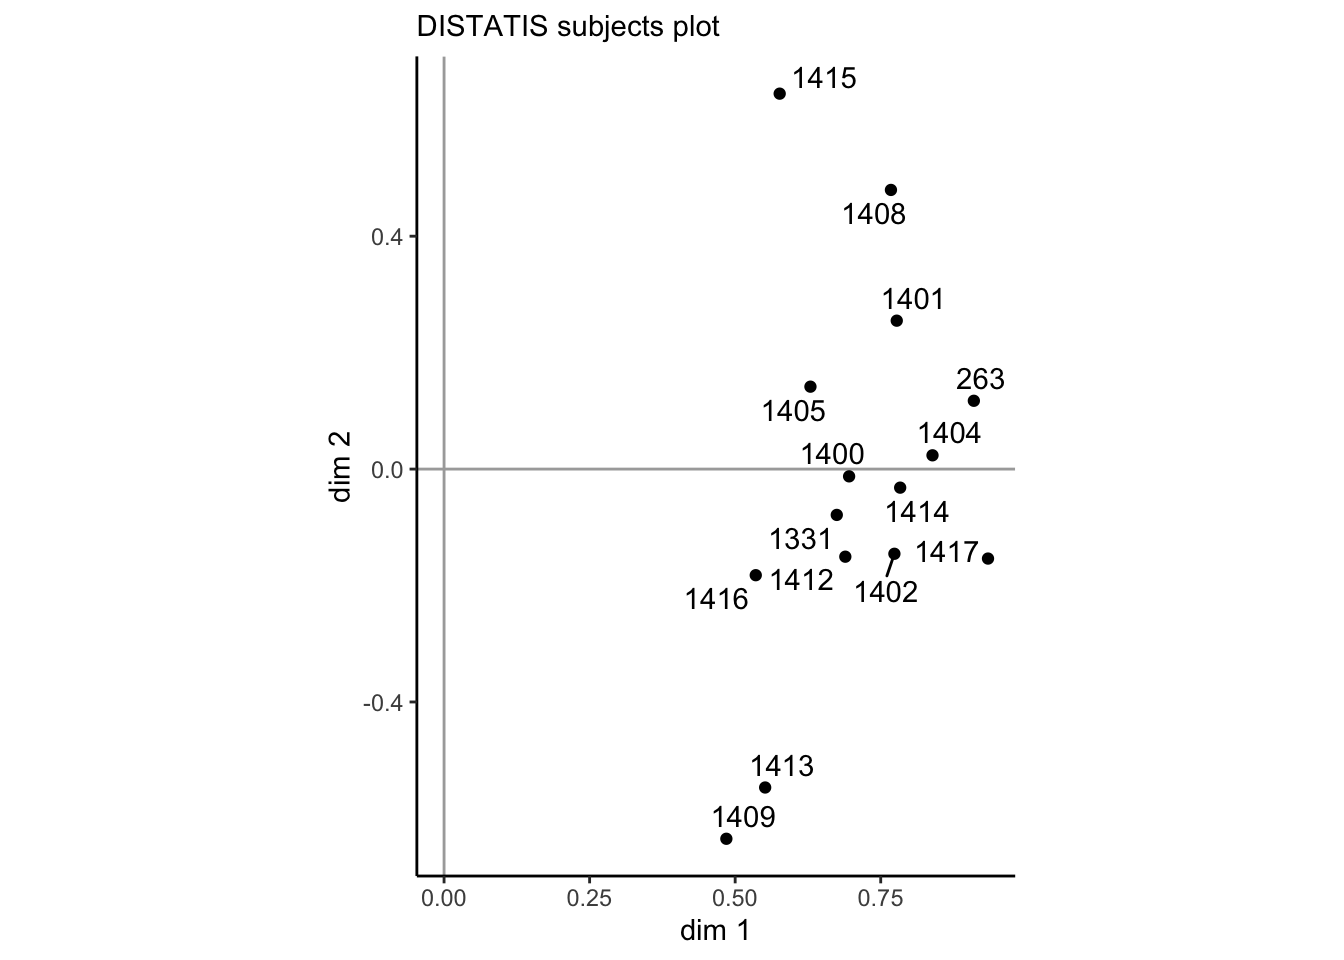
\includegraphics[keepaspectratio]{07-HCA_files/figure-latex/unnamed-chunk-11-1.pdf}}

Only single linkage gives us very different results; the others are a matter of scaling. This could be quite different if we had a larger number of more dissimilar objects - recall our distance matrix:

\begin{Shaded}
\begin{Highlighting}[]
\NormalTok{descriptive\_distance}
\end{Highlighting}
\end{Shaded}

\begin{verbatim}
##             C_MERLOT C_REFOSCO  C_SYRAH C_ZINFANDEL I_MERLOT I_PRIMITIVO
## C_REFOSCO   5.083950                                                    
## C_SYRAH     4.525147  5.472269                                          
## C_ZINFANDEL 3.909011  5.856348 4.817566                                 
## I_MERLOT    4.503404  6.405151 6.153529    6.522035                     
## I_PRIMITIVO 6.129930  7.853063 5.998705    5.543431 7.842528            
## I_REFOSCO   6.272963  6.992652 5.408757    6.917554 4.452965    8.514098
## I_SYRAH     6.911105  8.427799 6.359281    6.170264 7.546229    5.747512
##             I_REFOSCO
## C_REFOSCO            
## C_SYRAH              
## C_ZINFANDEL          
## I_MERLOT             
## I_PRIMITIVO          
## I_REFOSCO            
## I_SYRAH      7.537424
\end{verbatim}

Not actually that much variation!

We can do the same thing with our individual observations.

\begin{Shaded}
\begin{Highlighting}[]
\NormalTok{individual\_distances }\OtherTok{\textless{}{-}} 
\NormalTok{  descriptive\_data }\SpecialCharTok{\%\textgreater{}\%}
  \FunctionTok{unite}\NormalTok{(NJ, ProductName, NR, }\AttributeTok{col =} \StringTok{"ID"}\NormalTok{) }\SpecialCharTok{\%\textgreater{}\%}
  \FunctionTok{mutate}\NormalTok{(}\FunctionTok{across}\NormalTok{(}\FunctionTok{where}\NormalTok{(is.numeric), }\SpecialCharTok{\textasciitilde{}}\NormalTok{ (. }\SpecialCharTok{{-}} \FunctionTok{mean}\NormalTok{(.)) }\SpecialCharTok{/} \FunctionTok{sd}\NormalTok{(.))) }\SpecialCharTok{\%\textgreater{}\%}
  \FunctionTok{column\_to\_rownames}\NormalTok{(}\StringTok{"ID"}\NormalTok{) }\SpecialCharTok{\%\textgreater{}\%}
  \FunctionTok{dist}\NormalTok{()}

\NormalTok{clusters\_individual }\OtherTok{\textless{}{-}} 
\NormalTok{  individual\_distances }\SpecialCharTok{\%\textgreater{}\%}
  \FunctionTok{hclust}\NormalTok{(}\AttributeTok{method =} \StringTok{"ward.D2"}\NormalTok{)}

\CommentTok{\# Here we drop the original unique IDs for just the ProductName}
\NormalTok{clusters\_individual}\SpecialCharTok{$}\NormalTok{labels }\OtherTok{\textless{}{-}} \FunctionTok{str\_extract}\NormalTok{(clusters\_individual}\SpecialCharTok{$}\NormalTok{labels, }\StringTok{"[A{-}Z]\_[A{-}Z]+"}\NormalTok{)}

\NormalTok{p }\OtherTok{\textless{}{-}}\NormalTok{ clusters\_individual }\SpecialCharTok{\%\textgreater{}\%}
  \FunctionTok{fviz\_dend}\NormalTok{(}\AttributeTok{cex =} \DecValTok{1}\SpecialCharTok{/}\DecValTok{4}\NormalTok{,}
            \AttributeTok{k =} \DecValTok{8}\NormalTok{,}
            \AttributeTok{label\_cols =}\NormalTok{ clusters\_individual}\SpecialCharTok{$}\NormalTok{labels }\SpecialCharTok{\%\textgreater{}\%} \FunctionTok{as.factor}\NormalTok{() }\SpecialCharTok{\%\textgreater{}\%} \FunctionTok{as.numeric}\NormalTok{()) }\SpecialCharTok{+} 
  \FunctionTok{labs}\NormalTok{(}\AttributeTok{title =} \StringTok{"Clustering raw data with Ward\textquotesingle{}s method"}\NormalTok{) }\SpecialCharTok{+}
  \FunctionTok{scale\_color\_viridis\_d}\NormalTok{()}

\NormalTok{p}
\end{Highlighting}
\end{Shaded}

\pandocbounded{\includegraphics[keepaspectratio]{07-HCA_files/figure-latex/unnamed-chunk-13-1.pdf}}

We tried looking for 8 clusters (since there are 8 wines) and giving each label (the individual row observation representing a single judge rating a single wine sample) the color of the rated wine. It is obvious that the wines don't cluster together based on their sample ID.

\section{Using cluster IDs}\label{using-cluster-ids}

Above we played a little bit to see if, for the raw data, clustering provided a structure that mirrored product ID. But that was more for demonstration purposes than because it was a good data-analysis practice. More standard in sensory evaluation workflow would be to conduct a clustering analysis and then determine whether that cluster ``explained'' sensory variation in the base data.

From our original clustering results, we can pull out a tibble that tells us which sample belongs to which cluster:

\begin{Shaded}
\begin{Highlighting}[]
\CommentTok{\# We use \textasciigrave{}cutree()\textasciigrave{} with \textasciigrave{}k = 3\textasciigrave{} to get 3 groups from the "tree" (clustering)}
\NormalTok{groups\_from\_ward }\OtherTok{\textless{}{-}} 
\NormalTok{  cluster\_ward }\SpecialCharTok{\%\textgreater{}\%}
  \FunctionTok{cutree}\NormalTok{(}\AttributeTok{k =} \DecValTok{3}\NormalTok{) }\SpecialCharTok{\%\textgreater{}\%}
  \FunctionTok{as\_tibble}\NormalTok{(}\AttributeTok{rownames =} \StringTok{"ProductName"}\NormalTok{) }\SpecialCharTok{\%\textgreater{}\%}
  \FunctionTok{rename}\NormalTok{(}\AttributeTok{ward\_group =}\NormalTok{ value) }\SpecialCharTok{\%\textgreater{}\%}
  \CommentTok{\# It will be helpful to treat group membership as a nominal variable}
  \FunctionTok{mutate}\NormalTok{(}\AttributeTok{ward\_group =} \FunctionTok{factor}\NormalTok{(ward\_group))}

\CommentTok{\# The \textasciigrave{}dplyr::left\_join()\textasciigrave{} function matches up the two tibbles based on the}
\CommentTok{\# value of a shared column(s): in this case, \textasciigrave{}ProductName\textasciigrave{}}
\NormalTok{descriptive\_data }\OtherTok{\textless{}{-}} 
\NormalTok{  descriptive\_data }\SpecialCharTok{\%\textgreater{}\%}
  \FunctionTok{left\_join}\NormalTok{(groups\_from\_ward)}

\FunctionTok{glimpse}\NormalTok{(descriptive\_data)}
\end{Highlighting}
\end{Shaded}

\begin{verbatim}
## Rows: 336
## Columns: 24
## $ NJ              <fct> 1331, 1331, 1331, 1331, 1331, 1331, 1331, 1331, 1400, ~
## $ ProductName     <chr> "C_MERLOT", "C_SYRAH", "C_ZINFANDEL", "C_REFOSCO", "I_~
## $ NR              <fct> 7, 7, 7, 7, 7, 7, 7, 7, 7, 7, 7, 7, 7, 7, 7, 7, 7, 7, ~
## $ Red_berry       <dbl> 5.1, 5.6, 4.9, 5.0, 3.3, 5.7, 2.9, 3.2, 0.1, 1.6, 4.5,~
## $ Dark_berry      <dbl> 5.8, 1.9, 2.6, 1.9, 7.2, 3.6, 5.1, 6.0, 0.1, 0.7, 2.9,~
## $ Jam             <dbl> 2.1, 3.9, 1.4, 7.8, 0.5, 8.7, 8.7, 4.0, 0.2, 0.0, 0.3,~
## $ Dried_fruit     <dbl> 4.7, 1.2, 5.9, 0.6, 5.8, 1.9, 0.4, 0.7, 2.9, 6.4, 2.4,~
## $ Artificial_frui <dbl> 1.0, 7.9, 0.8, 6.6, 0.7, 7.4, 6.2, 4.1, 0.1, 0.1, 0.1,~
## $ Chocolate       <dbl> 2.9, 1.0, 2.0, 6.4, 2.1, 3.3, 3.4, 3.6, 0.2, 1.0, 0.2,~
## $ Vanilla         <dbl> 5.0, 8.3, 2.7, 5.5, 1.3, 6.9, 8.1, 4.8, 2.0, 0.8, 1.9,~
## $ Oak             <dbl> 5.0, 2.3, 5.6, 3.6, 2.1, 1.5, 1.8, 2.6, 3.0, 5.4, 6.1,~
## $ Burned          <dbl> 1.4, 1.8, 1.9, 3.2, 5.6, 0.2, 0.4, 4.7, 7.5, 5.1, 0.3,~
## $ Leather         <dbl> 2.3, 3.5, 4.3, 0.3, 6.5, 1.5, 4.1, 6.5, 0.7, 0.8, 0.2,~
## $ Earthy          <dbl> 0.6, 1.0, 0.6, 0.2, 4.7, 0.3, 0.5, 1.9, 0.7, 3.0, 1.3,~
## $ Spicy           <dbl> 3.2, 0.7, 1.4, 2.9, 0.7, 3.1, 0.7, 1.4, 0.3, 3.2, 3.1,~
## $ Pepper          <dbl> 5.4, 3.0, 4.1, 0.9, 2.8, 1.6, 3.6, 4.5, 0.1, 2.0, 0.9,~
## $ Grassy          <dbl> 2.1, 0.6, 3.6, 1.8, 3.8, 0.9, 2.3, 0.8, 0.1, 1.3, 0.4,~
## $ Medicinal       <dbl> 0.4, 2.2, 1.7, 0.2, 2.6, 0.5, 0.2, 3.8, 0.1, 2.1, 0.1,~
## $ `Band-aid`      <dbl> 0.4, 0.4, 0.1, 0.2, 5.1, 1.2, 0.2, 6.2, 0.1, 1.1, 0.1,~
## $ Sour            <dbl> 5.0, 9.7, 7.8, 8.3, 7.6, 7.2, 5.9, 6.3, 5.7, 6.4, 5.4,~
## $ Bitter          <dbl> 5.9, 5.2, 3.5, 3.0, 1.9, 9.8, 2.9, 0.2, 0.6, 2.9, 0.1,~
## $ Alcohol         <dbl> 9.0, 7.2, 4.7, 8.9, 2.8, 8.7, 1.6, 7.0, 1.6, 5.4, 4.9,~
## $ Astringent      <dbl> 8.7, 8.3, 5.0, 7.8, 5.9, 8.0, 2.6, 4.2, 5.5, 5.1, 5.9,~
## $ ward_group      <fct> 1, 1, 1, 1, 2, 3, 3, 2, 1, 1, 1, 1, 2, 3, 3, 2, 1, 1, ~
\end{verbatim}

Now we have a \texttt{factor} identifying which cluster (from an HCA with Ward's Method and 3 groups) each wine belongs to. We can use this structure as a new possible input for M/ANOVA, like we did in \hyperref[manova-multivariate-analysis-of-variance]{MANOVA (Multivariate Analysis of Variance)}.

\begin{Shaded}
\begin{Highlighting}[]
\NormalTok{cluster\_manova }\OtherTok{\textless{}{-}} 
  \FunctionTok{manova}\NormalTok{(}\AttributeTok{formula =} \FunctionTok{as.matrix}\NormalTok{(descriptive\_data[, }\DecValTok{4}\SpecialCharTok{:}\DecValTok{23}\NormalTok{]) }\SpecialCharTok{\textasciitilde{}}\NormalTok{ ward\_group, }
         \AttributeTok{data =}\NormalTok{ descriptive\_data)}

\CommentTok{\# We get a "significant" 1{-}way MANOVA result for the effect of cluster}
\CommentTok{\# membership on overall sensory profile.}
\FunctionTok{summary}\NormalTok{(cluster\_manova, }\AttributeTok{test =} \StringTok{"W"}\NormalTok{)}
\end{Highlighting}
\end{Shaded}

\begin{verbatim}
##             Df   Wilks approx F num Df den Df    Pr(>F)    
## ward_group   2 0.52896   5.8867     40    628 < 2.2e-16 ***
## Residuals  333                                             
## ---
## Signif. codes:  0 '***' 0.001 '**' 0.01 '*' 0.05 '.' 0.1 ' ' 1
\end{verbatim}

\begin{Shaded}
\begin{Highlighting}[]
\CommentTok{\# Let\textquotesingle{}s review how to use nest() and map() functions to tidily apply 1{-}way ANOVA}
\CommentTok{\# to each variable.}

\NormalTok{descriptive\_data }\SpecialCharTok{\%\textgreater{}\%}
  \CommentTok{\# We are going to ignore (marginalize) reps and judges and even products}
  \FunctionTok{select}\NormalTok{(}\SpecialCharTok{{-}}\NormalTok{NR, }\SpecialCharTok{{-}}\NormalTok{NJ, }\SpecialCharTok{{-}}\NormalTok{ProductName) }\SpecialCharTok{\%\textgreater{}\%}
  \FunctionTok{pivot\_longer}\NormalTok{(}\SpecialCharTok{{-}}\NormalTok{ward\_group,}
               \AttributeTok{names\_to =} \StringTok{"descriptor"}\NormalTok{,}
               \AttributeTok{values\_to =} \StringTok{"rating"}\NormalTok{) }\SpecialCharTok{\%\textgreater{}\%}
  \FunctionTok{nest}\NormalTok{(}\AttributeTok{data =} \SpecialCharTok{{-}}\NormalTok{descriptor) }\SpecialCharTok{\%\textgreater{}\%}
  \CommentTok{\# run 1{-}way ANOVAs}
  \FunctionTok{mutate}\NormalTok{(}\AttributeTok{anova\_results =} \FunctionTok{map}\NormalTok{(}\AttributeTok{.x =}\NormalTok{ data,}
                             \AttributeTok{.f =} \SpecialCharTok{\textasciitilde{}}\FunctionTok{aov}\NormalTok{(rating }\SpecialCharTok{\textasciitilde{}}\NormalTok{ ward\_group, }\AttributeTok{data =}\NormalTok{ .))) }\SpecialCharTok{\%\textgreater{}\%}
  \CommentTok{\# use broom::tidy() to get tibble{-}ized summaries out of the \textasciigrave{}aov\textasciigrave{} objects}
  \FunctionTok{transmute}\NormalTok{(descriptor,}
            \AttributeTok{tidy\_summary =} \FunctionTok{map}\NormalTok{(anova\_results, broom}\SpecialCharTok{::}\NormalTok{tidy)) }\SpecialCharTok{\%\textgreater{}\%}
  \FunctionTok{unnest}\NormalTok{(}\FunctionTok{everything}\NormalTok{()) }\SpecialCharTok{\%\textgreater{}\%}
  \FunctionTok{filter}\NormalTok{(term  }\SpecialCharTok{!=} \StringTok{"Residuals"}\NormalTok{,}
\NormalTok{         p.value }\SpecialCharTok{\textless{}} \FloatTok{0.05}\NormalTok{) }\SpecialCharTok{\%\textgreater{}\%}
  \FunctionTok{mutate}\NormalTok{(}\FunctionTok{across}\NormalTok{(}\FunctionTok{where}\NormalTok{(is.numeric), }\SpecialCharTok{\textasciitilde{}}\FunctionTok{round}\NormalTok{(., }\DecValTok{3}\NormalTok{))) }\SpecialCharTok{\%\textgreater{}\%}
  \FunctionTok{print}\NormalTok{(}\AttributeTok{n =} \DecValTok{13}\NormalTok{)}
\end{Highlighting}
\end{Shaded}

\begin{verbatim}
## # A tibble: 13 x 7
##    descriptor      term          df sumsq meansq statistic p.value
##    <chr>           <chr>      <dbl> <dbl>  <dbl>     <dbl>   <dbl>
##  1 Red_berry       ward_group     2  49.7  24.9       3.97   0.02 
##  2 Dark_berry      ward_group     2  81.5  40.8       5.54   0.004
##  3 Jam             ward_group     2 243.  122.       23.7    0    
##  4 Artificial_frui ward_group     2 134.   66.9      18.7    0    
##  5 Chocolate       ward_group     2  20.6  10.3       3.41   0.034
##  6 Vanilla         ward_group     2  59.6  29.8       7.74   0.001
##  7 Oak             ward_group     2  37.5  18.8       4.89   0.008
##  8 Burned          ward_group     2 106.   53.1      13.7    0    
##  9 Leather         ward_group     2  70.2  35.1       8.90   0    
## 10 Earthy          ward_group     2  20.0  10.0       4.18   0.016
## 11 Grassy          ward_group     2  16.6   8.28      4.07   0.018
## 12 Medicinal       ward_group     2 109.   54.4      14.7    0    
## 13 Band-aid        ward_group     2  96.5  48.3      12.4    0
\end{verbatim}

We find that 13 descriptors have significantly different means for the 3 different clusters. This seems to contradict HGH's results--she found 7 in the original \textbf{R Opus}. I am not quite sure what the difference could be here; when I reran the code from the actual original \textbf{R Opus} my results match the tidy workflow shown above (not shown). I wonder if some data got lost somewhere in the original?

\section{K-means clustering}\label{k-means-clustering}

In hierarchical clustering, we use an iterative process to merge our items into groups--if we let the process run long enough we end up with a single group. We decide on the ``right'' number of groups by examining results like the \emph{dendrogram} produced from the set of merges throughout the process (e.g., we apply \texttt{cutree(k\ =\ 3)}).

If we had some idea \emph{a priori} of how many groups we were expecting, we could use some alternative processes. The most popular--and possibly intuitive--of these is \emph{k-means clustering}. The \(k\) in ``k-means'' stands in for the same thing it does in the \texttt{k\ =} argument in \texttt{cutree()}: how many groups are we looking for. However, in k-means clustering, we don't proceed hierarchically. Instead, we start with some initial \(k\) ``seeds'' - the initial 1-item groups. These can be chosen at random or purposively, although if the former it is important to note that the choice of seed can be influential on the solution, and so multiple runs of k-means clustering may produce different results.

Once the \(k\) seeds are chosen, every other item that is to be clustered is assigned to the group for which it is closest to the seed (again, ``closest'' can be defined by any distance metric). Once a group has more than 1 item, its centroid (the ``mean'' in the name ``k-means'') replaces the initial seed for distance measurements. After an initial run, it is possible that items are in the ``wrong'' group--that a new, different group centroid is closer to them than is their current group centroid. These items are re-assigned, centroids are re-calculated, and the procedure iterates until no items are re-assigned. This reassignment is not possible with hierarchical methods, and so k-means can sometimes find better results. As might be imagined, different choices of methods for calculating centroid and for distance can affect the results of k-means clustering.

A common workflow is to use HCA to get an idea of the appropriate \(k\) for k-means clustering, and then to use k-means clustering to get a final, optimized clustering solution. We will take this approach, using \texttt{k\ =\ 3}.

\begin{Shaded}
\begin{Highlighting}[]
\NormalTok{clusters\_kmeans }\OtherTok{\textless{}{-}}
\NormalTok{  descriptive\_means\_scaled }\SpecialCharTok{\%\textgreater{}\%}
  \FunctionTok{column\_to\_rownames}\NormalTok{(}\StringTok{"ProductName"}\NormalTok{) }\SpecialCharTok{\%\textgreater{}\%}
  \FunctionTok{kmeans}\NormalTok{(}\AttributeTok{centers =} \DecValTok{3}\NormalTok{)}

\NormalTok{clusters\_kmeans}\SpecialCharTok{$}\NormalTok{cluster}
\end{Highlighting}
\end{Shaded}

\begin{verbatim}
##    C_MERLOT   C_REFOSCO     C_SYRAH C_ZINFANDEL    I_MERLOT I_PRIMITIVO 
##           3           3           3           3           2           1 
##   I_REFOSCO     I_SYRAH 
##           2           1
\end{verbatim}

\begin{Shaded}
\begin{Highlighting}[]
\NormalTok{clusters\_kmeans}\SpecialCharTok{$}\NormalTok{centers }\SpecialCharTok{\%\textgreater{}\%}
  \FunctionTok{as\_tibble}\NormalTok{(}\AttributeTok{rownames =} \StringTok{"cluster"}\NormalTok{)}
\end{Highlighting}
\end{Shaded}

\begin{verbatim}
## # A tibble: 3 x 21
##   cluster Red_berry Dark_berry    Jam Dried_fruit Artificial_frui Chocolate
##   <chr>       <dbl>      <dbl>  <dbl>       <dbl>           <dbl>     <dbl>
## 1 1           1.34       1.29   1.49       0.0234           1.58      0.179
## 2 2          -0.423     -0.629 -0.729      0.255           -0.544    -1.07 
## 3 3          -0.456     -0.328 -0.379     -0.139           -0.515     0.444
## # i 14 more variables: Vanilla <dbl>, Oak <dbl>, Burned <dbl>, Leather <dbl>,
## #   Earthy <dbl>, Spicy <dbl>, Pepper <dbl>, Grassy <dbl>, Medicinal <dbl>,
## #   `Band-aid` <dbl>, Sour <dbl>, Bitter <dbl>, Alcohol <dbl>, Astringent <dbl>
\end{verbatim}

HGH shows how to replicate the same workflow as we did above with the HCA results: using the group assignments to run a 1-way M/ANOVA to determine which attributes vary significantly. I am going to leave this as an exercise to the reader, but we'll instead look at how we might visualize these results, since we can't draw a dendrogram in the same way as an HCA.

We'll first run a simple means PCA to get the product score plot, and then we'll draw some hulls around the groups.

\begin{Shaded}
\begin{Highlighting}[]
\NormalTok{means\_pca }\OtherTok{\textless{}{-}} 
\NormalTok{  descriptive\_means }\SpecialCharTok{\%\textgreater{}\%}
  \FunctionTok{column\_to\_rownames}\NormalTok{(}\StringTok{"ProductName"}\NormalTok{) }\SpecialCharTok{\%\textgreater{}\%}
\NormalTok{  FactoMineR}\SpecialCharTok{::}\FunctionTok{PCA}\NormalTok{(}\AttributeTok{scale.unit =} \ConstantTok{FALSE}\NormalTok{, }\AttributeTok{graph =} \ConstantTok{FALSE}\NormalTok{)}

\CommentTok{\# Join the PCA scores to the k{-}means cluster IDs}
\NormalTok{p1 }\OtherTok{\textless{}{-}}
\NormalTok{  means\_pca}\SpecialCharTok{$}\NormalTok{ind}\SpecialCharTok{$}\NormalTok{coord }\SpecialCharTok{\%\textgreater{}\%}
  \FunctionTok{as\_tibble}\NormalTok{(}\AttributeTok{rownames =} \StringTok{"ProductName"}\NormalTok{) }\SpecialCharTok{\%\textgreater{}\%}
  \FunctionTok{left\_join}\NormalTok{(}
\NormalTok{    clusters\_kmeans}\SpecialCharTok{$}\NormalTok{cluster }\SpecialCharTok{\%\textgreater{}\%}
      \FunctionTok{as\_tibble}\NormalTok{(}\AttributeTok{rownames =} \StringTok{"ProductName"}\NormalTok{)}
\NormalTok{  ) }\SpecialCharTok{\%\textgreater{}\%}
  \FunctionTok{mutate}\NormalTok{(}\AttributeTok{value =} \FunctionTok{factor}\NormalTok{(value)) }\SpecialCharTok{\%\textgreater{}\%}
  \CommentTok{\# And plot!}
  \FunctionTok{ggplot}\NormalTok{(}\FunctionTok{aes}\NormalTok{(}\AttributeTok{x =}\NormalTok{ Dim}\FloatTok{.1}\NormalTok{, }\AttributeTok{y =}\NormalTok{ Dim}\FloatTok{.2}\NormalTok{)) }\SpecialCharTok{+} 
  \FunctionTok{geom\_hline}\NormalTok{(}\AttributeTok{yintercept =} \DecValTok{0}\NormalTok{, }\AttributeTok{linetype =} \DecValTok{2}\NormalTok{) }\SpecialCharTok{+} 
  \FunctionTok{geom\_vline}\NormalTok{(}\AttributeTok{xintercept =} \DecValTok{0}\NormalTok{, }\AttributeTok{linetype =} \DecValTok{2}\NormalTok{) }\SpecialCharTok{+} 
  \FunctionTok{geom\_point}\NormalTok{(}\FunctionTok{aes}\NormalTok{(}\AttributeTok{color =}\NormalTok{ value)) }\SpecialCharTok{+} 
\NormalTok{  ggrepel}\SpecialCharTok{::}\FunctionTok{geom\_text\_repel}\NormalTok{(}\FunctionTok{aes}\NormalTok{(}\AttributeTok{color =}\NormalTok{ value, }\AttributeTok{label =}\NormalTok{ ProductName)) }\SpecialCharTok{+} 
\NormalTok{  ggforce}\SpecialCharTok{::}\FunctionTok{geom\_mark\_ellipse}\NormalTok{(}\FunctionTok{aes}\NormalTok{(}\AttributeTok{color =}\NormalTok{ value)) }\SpecialCharTok{+} 
  \FunctionTok{theme\_bw}\NormalTok{() }\SpecialCharTok{+}
  \FunctionTok{coord\_equal}\NormalTok{() }\SpecialCharTok{+} 
  \FunctionTok{theme}\NormalTok{(}\AttributeTok{legend.position =} \StringTok{"none"}\NormalTok{)}
\NormalTok{p1}
\end{Highlighting}
\end{Shaded}

\pandocbounded{\includegraphics[keepaspectratio]{07-HCA_files/figure-latex/unnamed-chunk-17-1.pdf}}

Looks like those California wines end up grouped together even though there is a fair bit of spread. I looked into the PC3 to see if that explained it, but they are even more spread there (not shown--see if you can make the small code tweak to do so). I think this is a case where arguably 3 clusters is not a good solution. We might consider examining some measures of cluster fit, perhaps through something like the \texttt{NbClust} package, to determine if we should consider other solutions.

\section{Packages used in this chapter}\label{packages-used-in-this-chapter-6}

\begin{Shaded}
\begin{Highlighting}[]
\FunctionTok{sessionInfo}\NormalTok{()}
\end{Highlighting}
\end{Shaded}

\begin{verbatim}
## R version 4.4.1 (2024-06-14)
## Platform: x86_64-apple-darwin20
## Running under: macOS 15.2
## 
## Matrix products: default
## BLAS:   /Library/Frameworks/R.framework/Versions/4.4-x86_64/Resources/lib/libRblas.0.dylib 
## LAPACK: /Library/Frameworks/R.framework/Versions/4.4-x86_64/Resources/lib/libRlapack.dylib;  LAPACK version 3.12.0
## 
## locale:
## [1] en_US.UTF-8/en_US.UTF-8/en_US.UTF-8/C/en_US.UTF-8/en_US.UTF-8
## 
## time zone: America/New_York
## tzcode source: internal
## 
## attached base packages:
## [1] stats     graphics  grDevices datasets  utils     methods   base     
## 
## other attached packages:
##  [1] patchwork_1.2.0  factoextra_1.0.7 here_1.0.1       lubridate_1.9.3 
##  [5] forcats_1.0.0    stringr_1.5.1    dplyr_1.1.4      purrr_1.0.2     
##  [9] readr_2.1.5      tidyr_1.3.1      tibble_3.2.1     ggplot2_3.5.1   
## [13] tidyverse_2.0.0 
## 
## loaded via a namespace (and not attached):
##  [1] tidyselect_1.2.1     viridisLite_0.4.2    farver_2.1.2        
##  [4] viridis_0.6.5        fastmap_1.2.0        tweenr_2.0.3        
##  [7] digest_0.6.37        timechange_0.3.0     estimability_1.5.1  
## [10] lifecycle_1.0.4      cluster_2.1.6        multcompView_0.1-10 
## [13] magrittr_2.0.3       compiler_4.4.1       rlang_1.1.4         
## [16] tools_4.4.1          utf8_1.2.4           yaml_2.3.8          
## [19] knitr_1.46           ggsignif_0.6.4       labeling_0.4.3      
## [22] htmlwidgets_1.6.4    bit_4.0.5            scatterplot3d_0.3-44
## [25] abind_1.4-5          withr_3.0.0          grid_4.4.1          
## [28] polyclip_1.10-6      fansi_1.0.6          ggpubr_0.6.0        
## [31] xtable_1.8-4         colorspace_2.1-0     emmeans_1.10.2      
## [34] scales_1.3.0         MASS_7.3-60.2        flashClust_1.01-2   
## [37] cli_3.6.3            mvtnorm_1.2-5        rmarkdown_2.27      
## [40] crayon_1.5.2         generics_0.1.3       rstudioapi_0.16.0   
## [43] tzdb_0.4.0           ggforce_0.4.2        parallel_4.4.1      
## [46] vctrs_0.6.5          carData_3.0-5        bookdown_0.39       
## [49] car_3.1-2            hms_1.1.3            bit64_4.0.5         
## [52] rstatix_0.7.2        ggrepel_0.9.5        FactoMineR_2.11     
## [55] dendextend_1.17.1    glue_1.7.0           DT_0.33             
## [58] stringi_1.8.4        gtable_0.3.5         munsell_0.5.1       
## [61] pillar_1.9.0         htmltools_0.5.8.1    R6_2.5.1            
## [64] rprojroot_2.0.4      vroom_1.6.5          evaluate_0.23       
## [67] lattice_0.22-6       highr_0.10           backports_1.5.0     
## [70] leaps_3.1            broom_1.0.6          renv_1.0.9          
## [73] Rcpp_1.0.13          coda_0.19-4.1        gridExtra_2.3       
## [76] xfun_0.49            pkgconfig_2.0.3
\end{verbatim}

\chapter{Multidimensional Scaling (MDS)}\label{multidimensional-scaling-mds}

Multidimensional scaling (MDS) is a method of representing the distances among a set of items or observations. These distances can come originally from a high-dimensional space (such as the 20-dimensional space that defines our DA data), or from a low-dimensional space. Regardless, the goal of MDS is to find a low-dimensional (2- or 3-dimensional, usually) representation of the items in which the distances among the items is a close approximation of the original distance matrix.

You may notice that MDS operates on the same input data as the clustering techniques we just explored in the \hyperref[cluster-analysis]{previous chapter}. In clustering, the goal is not to find a metric or spatial arrangement of objects, but instead to determine some smaller number of \emph{clusters} or \emph{groups} that summarize or explain the observed distances among our samples. In MDS, the goal is to provide a visual and spatial representation of the distances.

In the \textbf{R Opus}, HGH applied MDS to the DA data. We'll explore the same approach once we review the key concept of metric and non-metric MDS.

\section{Metric vs non-metric}\label{metric-vs-non-metric}

Without going into details, MDS comes in two ``flavors'': metric and non-metric. In \textbf{metric MDS}, the distances among objects are taken as ``metric'' or measurement data: the units themselves are meaningful (another way of saying this is that they are \emph{interval} or \emph{ratio} data). In this case, the underlying algorithm for MDS is very similar to PCA, in which an eigendecomposition provides the optimal solution for finding a low-dimensional representation that explains the majority of the variations in distances among samples. Most sensory data is suitable for metric MDS, and in fact the \hyperref[distatis]{DISTATIS method we will use next} is predicated on a proof that distances even among sorting groups are metric (specifically, Euclidean).

For non-metric MDS, the assumption of the distances being meaningful metrics is relaxed; rather, we assume that the provided distances are only meaningful insofar as they represent ranks (they are \emph{ordinal} data). In this case, non-metric MDS uses a gradient-descent approach to find an approximation by extracting orthogonal dimensions while minimizing a criterion called \(STRESS\). Typically, we won't have to concern ourselves too much with non-metric MDS, but it could be useful when examining results from, for example, flash profiling (in which samples are ranked but not rated).

\section{Metric MDS}\label{metric-mds}

As usual, we begin by loading our required packages and the data.

\begin{Shaded}
\begin{Highlighting}[]
\FunctionTok{library}\NormalTok{(tidyverse)}
\FunctionTok{library}\NormalTok{(here)}

\NormalTok{descriptive\_data }\OtherTok{\textless{}{-}} 
  \FunctionTok{read\_csv}\NormalTok{(}\FunctionTok{here}\NormalTok{(}\StringTok{"data/torriDAFinal.csv"}\NormalTok{)) }\SpecialCharTok{\%\textgreater{}\%}
  \CommentTok{\# We\textquotesingle{}ll make some factors as usual}
  \FunctionTok{mutate}\NormalTok{(}\FunctionTok{across}\NormalTok{(}\DecValTok{1}\SpecialCharTok{:}\DecValTok{3}\NormalTok{, }\SpecialCharTok{\textasciitilde{}}\FunctionTok{as.factor}\NormalTok{(.)))}

\NormalTok{descriptive\_means }\OtherTok{\textless{}{-}} 
\NormalTok{  descriptive\_data }\SpecialCharTok{\%\textgreater{}\%}
  \CommentTok{\# Get the means for each wine and descriptor}
  \FunctionTok{group\_by}\NormalTok{(ProductName) }\SpecialCharTok{\%\textgreater{}\%}
  \FunctionTok{summarize}\NormalTok{(}\FunctionTok{across}\NormalTok{(}\FunctionTok{where}\NormalTok{(is.numeric), }\SpecialCharTok{\textasciitilde{}}\FunctionTok{mean}\NormalTok{(.))) }\SpecialCharTok{\%\textgreater{}\%}
  \CommentTok{\# Scale the data to unit variance}
  \FunctionTok{mutate}\NormalTok{(}\FunctionTok{across}\NormalTok{(}\FunctionTok{where}\NormalTok{(is.numeric), }\SpecialCharTok{\textasciitilde{}}\NormalTok{(. }\SpecialCharTok{{-}} \FunctionTok{mean}\NormalTok{(.)) }\SpecialCharTok{/} \FunctionTok{sd}\NormalTok{(.)))}
\end{Highlighting}
\end{Shaded}

Note that as in the previous chapter, HGH scales (normalizes) the data to \(\bar{x}=0\) and \(s=1\), which is a choice rather than a necessity for these methods. We will follow for consistency.

We then need to get the distances among all of our observations.

\begin{Shaded}
\begin{Highlighting}[]
\NormalTok{descriptive\_distances }\OtherTok{\textless{}{-}} 
\NormalTok{  descriptive\_means }\SpecialCharTok{\%\textgreater{}\%}
  \CommentTok{\# get the rownames as we go back to older functions }
  \FunctionTok{column\_to\_rownames}\NormalTok{(}\StringTok{"ProductName"}\NormalTok{) }\SpecialCharTok{\%\textgreater{}\%}
  \FunctionTok{dist}\NormalTok{(}\AttributeTok{method =} \StringTok{"euclidean"}\NormalTok{)}
\end{Highlighting}
\end{Shaded}

The \texttt{cmdscale()} function in the base \texttt{R} \texttt{stats} package will do metric MDS for us.

\begin{Shaded}
\begin{Highlighting}[]
\NormalTok{metric\_mds }\OtherTok{\textless{}{-}} 
\NormalTok{  descriptive\_distances }\SpecialCharTok{\%\textgreater{}\%}
  \CommentTok{\# \textasciigrave{}k\textasciigrave{} defines the \# of dimensions to extract, \textasciigrave{}eig\textasciigrave{} returns the eigenvalues}
  \CommentTok{\# for the spectral (eigen)decomposition}
  \FunctionTok{cmdscale}\NormalTok{(}\AttributeTok{k =} \DecValTok{2}\NormalTok{, }\AttributeTok{eig =} \ConstantTok{TRUE}\NormalTok{)}

\NormalTok{metric\_mds}
\end{Highlighting}
\end{Shaded}

\begin{verbatim}
## $points
##                    [,1]       [,2]
## C_MERLOT    -0.66017528 -1.4236819
## C_REFOSCO   -2.05394351 -3.2971758
## C_SYRAH     -0.08165706 -0.4392567
## C_ZINFANDEL  1.20071498 -1.5563951
## I_MERLOT    -2.87771919  1.5668345
## I_PRIMITIVO  4.11149279 -0.4593610
## I_REFOSCO   -3.14226246  2.8789771
## I_SYRAH      3.50354973  2.7300588
## 
## $eig
## [1] 5.343721e+01 3.392126e+01 1.755089e+01 1.363281e+01 1.225350e+01
## [6] 7.141861e+00 2.062458e+00 2.787237e-15
## 
## $x
## NULL
## 
## $ac
## [1] 0
## 
## $GOF
## [1] 0.6239891 0.6239891
\end{verbatim}

At this point you are familiar with our plot and wrangle approach - we're going to get that \texttt{\$points} table and pipe it into \texttt{ggplot2} to make a nicer looking plot.

\begin{Shaded}
\begin{Highlighting}[]
\NormalTok{p\_metric }\OtherTok{\textless{}{-}} 
\NormalTok{  metric\_mds}\SpecialCharTok{$}\NormalTok{points }\SpecialCharTok{\%\textgreater{}\%}
  \FunctionTok{as\_tibble}\NormalTok{(}\AttributeTok{rownames =} \StringTok{"sample"}\NormalTok{) }\SpecialCharTok{\%\textgreater{}\%}
  \FunctionTok{ggplot}\NormalTok{(}\FunctionTok{aes}\NormalTok{(}\AttributeTok{x =}\NormalTok{ V1, }\AttributeTok{y =}\NormalTok{ V2)) }\SpecialCharTok{+} 
  \FunctionTok{geom\_point}\NormalTok{() }\SpecialCharTok{+}
\NormalTok{  ggrepel}\SpecialCharTok{::}\FunctionTok{geom\_text\_repel}\NormalTok{(}\FunctionTok{aes}\NormalTok{(}\AttributeTok{label =}\NormalTok{ sample)) }\SpecialCharTok{+} 
  \FunctionTok{labs}\NormalTok{(}\AttributeTok{x =} \StringTok{"Dimension 1"}\NormalTok{, }\AttributeTok{y =} \StringTok{"Dimension 2"}\NormalTok{,}
       \AttributeTok{title =} \StringTok{"Metric MDS for wine DA data"}\NormalTok{) }\SpecialCharTok{+} 
  \FunctionTok{coord\_fixed}\NormalTok{() }\SpecialCharTok{+} 
  \FunctionTok{theme\_bw}\NormalTok{()}
\end{Highlighting}
\end{Shaded}

\begin{verbatim}
## Warning: The `x` argument of `as_tibble.matrix()` must have unique column names if
## `.name_repair` is omitted as of tibble 2.0.0.
## i Using compatibility `.name_repair`.
## This warning is displayed once every 8 hours.
## Call `lifecycle::last_lifecycle_warnings()` to see where this warning was
## generated.
\end{verbatim}

\begin{Shaded}
\begin{Highlighting}[]
\NormalTok{p\_metric}
\end{Highlighting}
\end{Shaded}

\pandocbounded{\includegraphics[keepaspectratio]{08-MDS_files/figure-latex/unnamed-chunk-4-1.pdf}}

We can also examine a scree-plot of the eigenvalues to get a (qualitative) view of this solution.

\begin{Shaded}
\begin{Highlighting}[]
\NormalTok{metric\_mds}\SpecialCharTok{$}\NormalTok{eig }\SpecialCharTok{\%\textgreater{}\%}
  \FunctionTok{as\_tibble}\NormalTok{() }\SpecialCharTok{\%\textgreater{}\%}
  \FunctionTok{mutate}\NormalTok{(}\AttributeTok{dim =} \FunctionTok{str\_c}\NormalTok{(}\StringTok{"Dimension "}\NormalTok{, }\FunctionTok{row\_number}\NormalTok{()),}
         \AttributeTok{value =}\NormalTok{ value }\SpecialCharTok{/} \FunctionTok{sum}\NormalTok{(value)) }\SpecialCharTok{\%\textgreater{}\%}
  \FunctionTok{ggplot}\NormalTok{(}\FunctionTok{aes}\NormalTok{(}\AttributeTok{x =}\NormalTok{ dim, }\AttributeTok{y =}\NormalTok{ value)) }\SpecialCharTok{+} 
  \FunctionTok{geom\_point}\NormalTok{() }\SpecialCharTok{+}
  \FunctionTok{geom\_line}\NormalTok{(}\FunctionTok{aes}\NormalTok{(}\AttributeTok{group =} \DecValTok{1}\NormalTok{)) }\SpecialCharTok{+} 
  \FunctionTok{theme\_bw}\NormalTok{() }\SpecialCharTok{+} 
  \FunctionTok{labs}\NormalTok{(}\AttributeTok{x =} \ConstantTok{NULL}\NormalTok{, }\AttributeTok{y =} \ConstantTok{NULL}\NormalTok{, }
       \AttributeTok{title =} \StringTok{"Scree plot for metric MDS"}\NormalTok{)}
\end{Highlighting}
\end{Shaded}

\pandocbounded{\includegraphics[keepaspectratio]{08-MDS_files/figure-latex/unnamed-chunk-5-1.pdf}}

We can see that, arguably, a 2-dimensional solution is not great for capturing the distances among these samples. See that bend \emph{after} the 3rd dimension? That's where we'd often want to put a cut. But this is a little academic - in practice we often only look at the first dimensions.

Let's compare the distances from our MDS solution to the actual distances:

\begin{Shaded}
\begin{Highlighting}[]
\CommentTok{\# Actual distances}
\NormalTok{descriptive\_distances}
\end{Highlighting}
\end{Shaded}

\begin{verbatim}
##             C_MERLOT C_REFOSCO  C_SYRAH C_ZINFANDEL I_MERLOT I_PRIMITIVO
## C_REFOSCO   5.083950                                                    
## C_SYRAH     4.525147  5.472269                                          
## C_ZINFANDEL 3.909011  5.856348 4.817566                                 
## I_MERLOT    4.503404  6.405151 6.153529    6.522035                     
## I_PRIMITIVO 6.129930  7.853063 5.998705    5.543431 7.842528            
## I_REFOSCO   6.272963  6.992652 5.408757    6.917554 4.452965    8.514098
## I_SYRAH     6.911105  8.427799 6.359281    6.170264 7.546229    5.747512
##             I_REFOSCO
## C_REFOSCO            
## C_SYRAH              
## C_ZINFANDEL          
## I_MERLOT             
## I_PRIMITIVO          
## I_REFOSCO            
## I_SYRAH      7.537424
\end{verbatim}

\begin{Shaded}
\begin{Highlighting}[]
\CommentTok{\# Approximate distances}
\NormalTok{metric\_mds}\SpecialCharTok{$}\NormalTok{points }\SpecialCharTok{\%\textgreater{}\%}
  \FunctionTok{dist}\NormalTok{(}\AttributeTok{method =} \StringTok{"euclidean"}\NormalTok{)}
\end{Highlighting}
\end{Shaded}

\begin{verbatim}
##             C_MERLOT C_REFOSCO  C_SYRAH C_ZINFANDEL I_MERLOT I_PRIMITIVO
## C_REFOSCO   2.335074                                                    
## C_SYRAH     1.141830  3.472408                                          
## C_ZINFANDEL 1.865617  3.690951 1.700728                                 
## I_MERLOT    3.722995  4.933275 3.441274    5.136944                     
## I_PRIMITIVO 4.868134  6.787179 4.193198    3.110645 7.276988            
## I_REFOSCO   4.967256  6.271308 4.514198    6.207574 1.338544    7.985078
## I_SYRAH     5.881341  8.198371 4.785214    4.865875 6.486423    3.246844
##             I_REFOSCO
## C_REFOSCO            
## C_SYRAH              
## C_ZINFANDEL          
## I_MERLOT             
## I_PRIMITIVO          
## I_REFOSCO            
## I_SYRAH      6.647480
\end{verbatim}

Here we can see that the distances are indeed only approximate (and not that good an approximation).

Would this get better if we went up to 3 dimensions? We can answer that pretty easily:

\begin{Shaded}
\begin{Highlighting}[]
\NormalTok{descriptive\_distances }\SpecialCharTok{\%\textgreater{}\%}
  \FunctionTok{cmdscale}\NormalTok{(}\AttributeTok{k =} \DecValTok{3}\NormalTok{, }\AttributeTok{eig =} \ConstantTok{TRUE}\NormalTok{) }\SpecialCharTok{\%\textgreater{}\%}
\NormalTok{  .}\SpecialCharTok{$}\NormalTok{points }\SpecialCharTok{\%\textgreater{}\%}
  \FunctionTok{dist}\NormalTok{()}
\end{Highlighting}
\end{Shaded}

\begin{verbatim}
##             C_MERLOT C_REFOSCO  C_SYRAH C_ZINFANDEL I_MERLOT I_PRIMITIVO
## C_REFOSCO   3.882087                                                    
## C_SYRAH     3.867494  3.522813                                          
## C_ZINFANDEL 2.323006  4.070842 2.869323                                 
## I_MERLOT    3.775222  6.182909 5.523805    5.516157                     
## I_PRIMITIVO 4.910980  7.217195 5.183820    3.196724 7.387510            
## I_REFOSCO   5.696284  6.279119 4.604395    6.364382 3.667013    8.267098
## I_SYRAH     6.453639  8.210405 4.896535    5.029587 7.269797    3.818459
##             I_REFOSCO
## C_REFOSCO            
## C_SYRAH              
## C_ZINFANDEL          
## I_MERLOT             
## I_PRIMITIVO          
## I_REFOSCO            
## I_SYRAH      6.648776
\end{verbatim}

It does look like we're getting closer to the original distances as we go up in dimensionality - the algorithm is able to find ``space'' to place the points further apart.

Let's examine one more thing that will lead us to \emph{non}-metric MDS: does our 2-dimensional MDS solution capture the correct \emph{rank order} of distances? In other words, is each pairwise distance in the MDS approximation in the same \emph{order} as it would be in the actual distance matrix?

\begin{Shaded}
\begin{Highlighting}[]
\CommentTok{\# I am getting sick of manually tidying distance matrices, so we\textquotesingle{}re going to}
\CommentTok{\# enlist the \textasciigrave{}widyr\textasciigrave{} package to automate this.}
\FunctionTok{library}\NormalTok{(widyr)}

\CommentTok{\# Of course this creates a new set of needs, including getting our data into a}
\CommentTok{\# tidy format to start with}
\NormalTok{tidy\_descriptive\_distances }\OtherTok{\textless{}{-}} 
\NormalTok{  descriptive\_means }\SpecialCharTok{\%\textgreater{}\%}
  \FunctionTok{pivot\_longer}\NormalTok{(}\SpecialCharTok{{-}}\NormalTok{ProductName,}
               \AttributeTok{names\_to =} \StringTok{"descriptor"}\NormalTok{,}
               \AttributeTok{values\_to =} \StringTok{"rating"}\NormalTok{) }\SpecialCharTok{\%\textgreater{}\%}
  \FunctionTok{arrange}\NormalTok{(ProductName) }\SpecialCharTok{\%\textgreater{}\%}
  \CommentTok{\# The distance between \textasciigrave{}ProductName\textasciigrave{}, based on \textasciigrave{}descriptor\textasciigrave{}, with values}
  \CommentTok{\# stored in \textasciigrave{}rating\textasciigrave{}}
  \FunctionTok{pairwise\_dist}\NormalTok{(}\AttributeTok{item =}\NormalTok{ ProductName, }\AttributeTok{feature =}\NormalTok{ descriptor, }\AttributeTok{value =}\NormalTok{ rating,}
                \AttributeTok{upper =} \ConstantTok{FALSE}\NormalTok{, }\AttributeTok{method =} \StringTok{"euclidean"}\NormalTok{)}

\FunctionTok{head}\NormalTok{(tidy\_descriptive\_distances)}
\end{Highlighting}
\end{Shaded}

\begin{verbatim}
## # A tibble: 6 x 3
##   item1     item2       distance
##   <fct>     <fct>          <dbl>
## 1 C_MERLOT  C_REFOSCO       5.08
## 2 C_MERLOT  C_SYRAH         4.53
## 3 C_REFOSCO C_SYRAH         5.47
## 4 C_MERLOT  C_ZINFANDEL     3.91
## 5 C_REFOSCO C_ZINFANDEL     5.86
## 6 C_SYRAH   C_ZINFANDEL     4.82
\end{verbatim}

\begin{Shaded}
\begin{Highlighting}[]
\CommentTok{\# We\textquotesingle{}ll do the same thing with our MDS results}
\NormalTok{tidy\_mds\_distances }\OtherTok{\textless{}{-}} 
\NormalTok{  metric\_mds}\SpecialCharTok{$}\NormalTok{points }\SpecialCharTok{\%\textgreater{}\%}
  \FunctionTok{as\_tibble}\NormalTok{(}\AttributeTok{rownames =} \StringTok{"product"}\NormalTok{) }\SpecialCharTok{\%\textgreater{}\%}
  \FunctionTok{arrange}\NormalTok{(product) }\SpecialCharTok{\%\textgreater{}\%}
  \FunctionTok{pivot\_longer}\NormalTok{(}\SpecialCharTok{{-}}\NormalTok{product) }\SpecialCharTok{\%\textgreater{}\%}
  \FunctionTok{pairwise\_dist}\NormalTok{(}\AttributeTok{item =}\NormalTok{ product, }\AttributeTok{feature =}\NormalTok{ name, }\AttributeTok{value =}\NormalTok{ value,}
                \AttributeTok{upper =} \ConstantTok{FALSE}\NormalTok{, }\AttributeTok{method =} \StringTok{"euclidean"}\NormalTok{)}

\FunctionTok{head}\NormalTok{(tidy\_mds\_distances)}
\end{Highlighting}
\end{Shaded}

\begin{verbatim}
## # A tibble: 6 x 3
##   item1     item2       distance
##   <chr>     <chr>          <dbl>
## 1 C_MERLOT  C_REFOSCO       2.34
## 2 C_MERLOT  C_SYRAH         1.14
## 3 C_REFOSCO C_SYRAH         3.47
## 4 C_MERLOT  C_ZINFANDEL     1.87
## 5 C_REFOSCO C_ZINFANDEL     3.69
## 6 C_SYRAH   C_ZINFANDEL     1.70
\end{verbatim}

We can now look at the ranks of pairwise distances and see how many are misaligned.

\begin{Shaded}
\begin{Highlighting}[]
\CommentTok{\# We will rank the pairwise distances from the original data}
\NormalTok{distance\_rankings }\OtherTok{\textless{}{-}}
\NormalTok{  tidy\_descriptive\_distances }\SpecialCharTok{\%\textgreater{}\%}
  \FunctionTok{unite}\NormalTok{(item1, item2, }\AttributeTok{col =} \StringTok{"items"}\NormalTok{, }\AttributeTok{sep =} \StringTok{" \textless{}{-}{-}\textgreater{} "}\NormalTok{) }\SpecialCharTok{\%\textgreater{}\%}
  \FunctionTok{transmute}\NormalTok{(items,}
            \AttributeTok{desc\_distance\_rank =} \FunctionTok{dense\_rank}\NormalTok{(distance)) }\SpecialCharTok{\%\textgreater{}\%}
  \FunctionTok{arrange}\NormalTok{(items) }\SpecialCharTok{\%\textgreater{}\%}
  \CommentTok{\# And now we\textquotesingle{}ll line this up with the MDS results}
  \FunctionTok{left\_join}\NormalTok{(}
\NormalTok{    tidy\_mds\_distances }\SpecialCharTok{\%\textgreater{}\%}
      \FunctionTok{unite}\NormalTok{(item1, item2, }\AttributeTok{col =} \StringTok{"items"}\NormalTok{, }\AttributeTok{sep =} \StringTok{" \textless{}{-}{-}\textgreater{} "}\NormalTok{) }\SpecialCharTok{\%\textgreater{}\%}
      \FunctionTok{transmute}\NormalTok{(items,}
                \AttributeTok{mds\_distance\_rank =} \FunctionTok{dense\_rank}\NormalTok{(distance)) }\SpecialCharTok{\%\textgreater{}\%}
      \FunctionTok{arrange}\NormalTok{(items),}
    \CommentTok{\# This is the line that lines them up (\textasciigrave{}by = \textasciigrave{})}
    \AttributeTok{by =} \StringTok{"items"}\NormalTok{)}

\NormalTok{distance\_rankings}
\end{Highlighting}
\end{Shaded}

\begin{verbatim}
## # A tibble: 28 x 3
##    items                      desc_distance_rank mds_distance_rank
##    <chr>                                   <int>             <int>
##  1 C_MERLOT <--> C_REFOSCO                     6                 5
##  2 C_MERLOT <--> C_SYRAH                       4                 1
##  3 C_MERLOT <--> C_ZINFANDEL                   1                 4
##  4 C_MERLOT <--> I_MERLOT                      3                11
##  5 C_MERLOT <--> I_PRIMITIVO                  13                16
##  6 C_MERLOT <--> I_REFOSCO                    16                18
##  7 C_MERLOT <--> I_SYRAH                      20                20
##  8 C_REFOSCO <--> C_SYRAH                      8                 9
##  9 C_REFOSCO <--> C_ZINFANDEL                 11                10
## 10 C_REFOSCO <--> I_MERLOT                    18                17
## # i 18 more rows
\end{verbatim}

\begin{Shaded}
\begin{Highlighting}[]
  \CommentTok{\# And finally we\textquotesingle{}ll check which are the same}
\NormalTok{distance\_rankings }\SpecialCharTok{\%\textgreater{}\%}
  \FunctionTok{mutate}\NormalTok{(}\AttributeTok{match =}\NormalTok{ desc\_distance\_rank }\SpecialCharTok{==}\NormalTok{ mds\_distance\_rank) }\SpecialCharTok{\%\textgreater{}\%}
  \FunctionTok{count}\NormalTok{(match)}
\end{Highlighting}
\end{Shaded}

\begin{verbatim}
## # A tibble: 2 x 2
##   match     n
##   <lgl> <int>
## 1 FALSE    21
## 2 TRUE      7
\end{verbatim}

That's actually very bad! We see only 1/4 of the original distances captured by the 2-dimensional MDS solution. Yikes.

Let's take a look and see if a non-metric MDS can do better.

\section{Non-metric MDS}\label{non-metric-mds}

In non-metric MDS, we assume that the observed distances are non-metric: they only represent an \emph{ordination} of the distances among the items. An example would be, in our actual data, that the observed distances represent estimates or opinions from our panelists:

\begin{Shaded}
\begin{Highlighting}[]
\NormalTok{tidy\_descriptive\_distances }\SpecialCharTok{\%\textgreater{}\%}
  \FunctionTok{arrange}\NormalTok{(distance)}
\end{Highlighting}
\end{Shaded}

\begin{verbatim}
## # A tibble: 28 x 3
##    item1       item2       distance
##    <fct>       <fct>          <dbl>
##  1 C_MERLOT    C_ZINFANDEL     3.91
##  2 I_MERLOT    I_REFOSCO       4.45
##  3 C_MERLOT    I_MERLOT        4.50
##  4 C_MERLOT    C_SYRAH         4.53
##  5 C_SYRAH     C_ZINFANDEL     4.82
##  6 C_MERLOT    C_REFOSCO       5.08
##  7 C_SYRAH     I_REFOSCO       5.41
##  8 C_REFOSCO   C_SYRAH         5.47
##  9 C_ZINFANDEL I_PRIMITIVO     5.54
## 10 I_PRIMITIVO I_SYRAH         5.75
## # i 18 more rows
\end{verbatim}

The closest samples are \texttt{C\_MERLOT} and \texttt{C\_ZINFANDEL}, and the second closest are \texttt{I\_MERLOT} and \texttt{I\_REFOSCO}. If our distances are merely ordinations, we can only say that--we can't compare the actual ``differences of distances'' as we could if these were metric. In the metric case, we could subtract the distance between \texttt{C\_MERLOT} and \texttt{C\_ZINFANDEL} and \texttt{I\_MERLOT} and \texttt{I\_REFOSCO} (\(\approx4.5-3.9\approx0.6\)) and say that the difference between those distances is larger than that between the second and third smallest distances (\texttt{I\_MERLOT} and \texttt{I\_REFOSCO} vs \texttt{C\_MERLOT} and \texttt{I\_MERLOT}, which is \(\approx4.5-4.45\approx0\)). So we could say something like ``the difference between the two closest pairs of samples is quite large, but the difference between the next two closest is approximately the same''. We can't do that with an ordination, because we only know the relative ranks:

\begin{Shaded}
\begin{Highlighting}[]
\NormalTok{tidy\_descriptive\_distances }\SpecialCharTok{\%\textgreater{}\%}
  \FunctionTok{transmute}\NormalTok{(item1, item2, }
            \AttributeTok{distance\_rank =} \FunctionTok{dense\_rank}\NormalTok{(distance)) }\SpecialCharTok{\%\textgreater{}\%}
  \FunctionTok{arrange}\NormalTok{(distance\_rank)}
\end{Highlighting}
\end{Shaded}

\begin{verbatim}
## # A tibble: 28 x 3
##    item1       item2       distance_rank
##    <fct>       <fct>               <int>
##  1 C_MERLOT    C_ZINFANDEL             1
##  2 I_MERLOT    I_REFOSCO               2
##  3 C_MERLOT    I_MERLOT                3
##  4 C_MERLOT    C_SYRAH                 4
##  5 C_SYRAH     C_ZINFANDEL             5
##  6 C_MERLOT    C_REFOSCO               6
##  7 C_SYRAH     I_REFOSCO               7
##  8 C_REFOSCO   C_SYRAH                 8
##  9 C_ZINFANDEL I_PRIMITIVO             9
## 10 I_PRIMITIVO I_SYRAH                10
## # i 18 more rows
\end{verbatim}

We can no longer know if the difference between 1st and 2nd place (so to speak, of \texttt{distance\_rank}) is the same as the difference between 2nd and 3rd place, and so on. We only know that \texttt{C\_MERLOT} and \texttt{C\_ZINFANDEL} are closer than \texttt{I\_MERLOT} and \texttt{I\_REFOSCO}, and so on.

OK, with that out of the way, let's take a look at non-metric MDS. For this, we will use the \texttt{MASS} package. \texttt{MASS} is bundled with \texttt{R}, but is not loaded by default. It contains many useful core functions for statistics, especially non-linear and multivariate stats. You can learn more about it \href{https://www.stats.ox.ac.uk/pub/MASS4/}{at the authors' website}.

\begin{Shaded}
\begin{Highlighting}[]
\FunctionTok{library}\NormalTok{(MASS)}

\CommentTok{\# the \textasciigrave{}isoMDS()\textasciigrave{} function will be what we use.}

\NormalTok{nonmetric\_mds }\OtherTok{\textless{}{-}}
  \FunctionTok{isoMDS}\NormalTok{(}\AttributeTok{d =}\NormalTok{ descriptive\_distances, }\AttributeTok{k =} \DecValTok{2}\NormalTok{)}
\end{Highlighting}
\end{Shaded}

\begin{verbatim}
## initial  value 9.444389 
## iter   5 value 7.065995
## iter  10 value 6.940918
## final  value 6.928604 
## converged
\end{verbatim}

As mentioned, non-metric MDS is an iterative optimization problem. We are told that the solution has ``converged'' because the \(STRESS\) value is no longer going down with subsequent iterations. Let's look at our results.

\begin{Shaded}
\begin{Highlighting}[]
\NormalTok{p\_nonmetric }\OtherTok{\textless{}{-}}
\NormalTok{  nonmetric\_mds}\SpecialCharTok{$}\NormalTok{points }\SpecialCharTok{\%\textgreater{}\%}
  \FunctionTok{as\_tibble}\NormalTok{(}\AttributeTok{rownames =} \StringTok{"sample"}\NormalTok{) }\SpecialCharTok{\%\textgreater{}\%}
  \FunctionTok{ggplot}\NormalTok{(}\FunctionTok{aes}\NormalTok{(}\AttributeTok{x =}\NormalTok{ V1, }\AttributeTok{y =}\NormalTok{ V2)) }\SpecialCharTok{+} 
  \FunctionTok{geom\_point}\NormalTok{() }\SpecialCharTok{+}
\NormalTok{  ggrepel}\SpecialCharTok{::}\FunctionTok{geom\_text\_repel}\NormalTok{(}\FunctionTok{aes}\NormalTok{(}\AttributeTok{label =}\NormalTok{ sample)) }\SpecialCharTok{+} 
  \FunctionTok{labs}\NormalTok{(}\AttributeTok{x =} \StringTok{"Dimension 1"}\NormalTok{, }\AttributeTok{y =} \StringTok{"Dimension 2"}\NormalTok{,}
       \AttributeTok{title =} \StringTok{"Non{-}metric MDS for wine DA data"}\NormalTok{) }\SpecialCharTok{+} 
  \FunctionTok{coord\_fixed}\NormalTok{() }\SpecialCharTok{+} 
  \FunctionTok{theme\_bw}\NormalTok{()}

\NormalTok{p\_nonmetric}
\end{Highlighting}
\end{Shaded}

\pandocbounded{\includegraphics[keepaspectratio]{08-MDS_files/figure-latex/unnamed-chunk-13-1.pdf}}

I'd like to compare our metric and non-metric configurations. To do so we can use the \texttt{patchwork} package, as we have before.

\begin{Shaded}
\begin{Highlighting}[]
\FunctionTok{library}\NormalTok{(patchwork)}

\NormalTok{p\_metric }\SpecialCharTok{+}\NormalTok{ p\_nonmetric}
\end{Highlighting}
\end{Shaded}

\pandocbounded{\includegraphics[keepaspectratio]{08-MDS_files/figure-latex/unnamed-chunk-14-1.pdf}}

Note that the configurations are quite similar, but with some notable shifts (e.g., the positioning of \texttt{I\_MERLOT} pops out). This makes sense: if you read the \texttt{?isoMDS} documentation, you'll see that the initial configuration for the non-metric MDS \emph{is} the metric MDS solution, so this approach starts with our metric MDS configuration and improves on it.

Let's see if we've improved the representation of our relative ranks for distances:

\begin{Shaded}
\begin{Highlighting}[]
\NormalTok{tidy\_nonmetric\_mds\_distances }\OtherTok{\textless{}{-}} 
\NormalTok{  nonmetric\_mds}\SpecialCharTok{$}\NormalTok{points }\SpecialCharTok{\%\textgreater{}\%}
  \FunctionTok{as\_tibble}\NormalTok{(}\AttributeTok{rownames =} \StringTok{"product"}\NormalTok{) }\SpecialCharTok{\%\textgreater{}\%}
  \FunctionTok{arrange}\NormalTok{(product) }\SpecialCharTok{\%\textgreater{}\%}
  \FunctionTok{pivot\_longer}\NormalTok{(}\SpecialCharTok{{-}}\NormalTok{product) }\SpecialCharTok{\%\textgreater{}\%}
  \FunctionTok{pairwise\_dist}\NormalTok{(}\AttributeTok{item =}\NormalTok{ product, }\AttributeTok{feature =}\NormalTok{ name, }\AttributeTok{value =}\NormalTok{ value,}
                \AttributeTok{upper =} \ConstantTok{FALSE}\NormalTok{, }\AttributeTok{method =} \StringTok{"euclidean"}\NormalTok{)}

\NormalTok{tidy\_descriptive\_distances }\SpecialCharTok{\%\textgreater{}\%}
  \FunctionTok{unite}\NormalTok{(item1, item2, }\AttributeTok{col =} \StringTok{"items"}\NormalTok{, }\AttributeTok{sep =} \StringTok{" \textless{}{-}{-}\textgreater{} "}\NormalTok{) }\SpecialCharTok{\%\textgreater{}\%}
  \FunctionTok{transmute}\NormalTok{(}\AttributeTok{observed\_rank =}\NormalTok{ items,}
            \AttributeTok{distance\_rank =} \FunctionTok{dense\_rank}\NormalTok{(distance)) }\SpecialCharTok{\%\textgreater{}\%}
  \FunctionTok{arrange}\NormalTok{(distance\_rank) }\SpecialCharTok{\%\textgreater{}\%}
  \CommentTok{\# And now we\textquotesingle{}ll line this up with the MDS results}
  \FunctionTok{left\_join}\NormalTok{(}
\NormalTok{    tidy\_nonmetric\_mds\_distances }\SpecialCharTok{\%\textgreater{}\%}
      \FunctionTok{unite}\NormalTok{(item1, item2, }\AttributeTok{col =} \StringTok{"items"}\NormalTok{, }\AttributeTok{sep =} \StringTok{" \textless{}{-}{-}\textgreater{} "}\NormalTok{) }\SpecialCharTok{\%\textgreater{}\%}
      \FunctionTok{transmute}\NormalTok{(}\AttributeTok{mds\_rank =}\NormalTok{ items,}
                \AttributeTok{distance\_rank =} \FunctionTok{dense\_rank}\NormalTok{(distance)) }\SpecialCharTok{\%\textgreater{}\%}
      \FunctionTok{arrange}\NormalTok{(distance\_rank),}
    \CommentTok{\# This is the line that lines them up (\textasciigrave{}by = \textasciigrave{})}
    \AttributeTok{by =} \StringTok{"distance\_rank"}
\NormalTok{  ) }\SpecialCharTok{\%\textgreater{}\%}
  \CommentTok{\# And finally we\textquotesingle{}ll check which are the same}
  \FunctionTok{mutate}\NormalTok{(}\AttributeTok{match =}\NormalTok{ observed\_rank }\SpecialCharTok{==}\NormalTok{ mds\_rank) }\SpecialCharTok{\%\textgreater{}\%}
  \FunctionTok{count}\NormalTok{(match)}
\end{Highlighting}
\end{Shaded}

\begin{verbatim}
## # A tibble: 2 x 2
##   match     n
##   <lgl> <int>
## 1 FALSE    25
## 2 TRUE      3
\end{verbatim}

It certainly doesn't seem like we have! Yikes! I think a higher-dimensional solution is certainly required to adequately capture the configuration of these products.

\section{Wrap up}\label{wrap-up}

To be fair, saying ``Yikes!'' is probably a little overblown. If we examined the tables above I used to compare the observed and estimated ranks in more detail, we'd see that the variation is quite small, for example, for the non-metric data:

\begin{verbatim}
## # A tibble: 28 x 4
##    observed_rank                distance_rank mds_rank                     match
##    <chr>                                <int> <chr>                        <lgl>
##  1 C_MERLOT <--> C_ZINFANDEL                1 C_MERLOT <--> C_ZINFANDEL    TRUE 
##  2 I_MERLOT <--> I_REFOSCO                  2 C_SYRAH <--> C_ZINFANDEL     FALSE
##  3 C_MERLOT <--> I_MERLOT                   3 C_MERLOT <--> C_SYRAH        FALSE
##  4 C_MERLOT <--> C_SYRAH                    4 I_MERLOT <--> I_REFOSCO      FALSE
##  5 C_SYRAH <--> C_ZINFANDEL                 5 C_MERLOT <--> I_MERLOT       FALSE
##  6 C_MERLOT <--> C_REFOSCO                  6 C_MERLOT <--> C_REFOSCO      TRUE 
##  7 C_SYRAH <--> I_REFOSCO                   7 C_ZINFANDEL <--> I_PRIMITIVO FALSE
##  8 C_REFOSCO <--> C_SYRAH                   8 C_SYRAH <--> I_MERLOT        FALSE
##  9 C_ZINFANDEL <--> I_PRIMITIVO             9 C_REFOSCO <--> I_MERLOT      FALSE
## 10 I_PRIMITIVO <--> I_SYRAH                10 C_REFOSCO <--> C_ZINFANDEL   FALSE
## # i 18 more rows
\end{verbatim}

As we can see, while indeed there are rank reversals, they are relatively minor: it isn't like samples that are close in the actual distance matrix are ending up being very far in the non-metric MDS 2-dimensional solution.

\section{Packages used in this chapter}\label{packages-used-in-this-chapter-7}

\begin{Shaded}
\begin{Highlighting}[]
\FunctionTok{sessionInfo}\NormalTok{()}
\end{Highlighting}
\end{Shaded}

\begin{verbatim}
## R version 4.4.1 (2024-06-14)
## Platform: x86_64-apple-darwin20
## Running under: macOS 15.2
## 
## Matrix products: default
## BLAS:   /Library/Frameworks/R.framework/Versions/4.4-x86_64/Resources/lib/libRblas.0.dylib 
## LAPACK: /Library/Frameworks/R.framework/Versions/4.4-x86_64/Resources/lib/libRlapack.dylib;  LAPACK version 3.12.0
## 
## locale:
## [1] en_US.UTF-8/en_US.UTF-8/en_US.UTF-8/C/en_US.UTF-8/en_US.UTF-8
## 
## time zone: America/New_York
## tzcode source: internal
## 
## attached base packages:
## [1] stats     graphics  grDevices datasets  utils     methods   base     
## 
## other attached packages:
##  [1] patchwork_1.2.0 MASS_7.3-60.2   widyr_0.1.5     here_1.0.1     
##  [5] lubridate_1.9.3 forcats_1.0.0   stringr_1.5.1   dplyr_1.1.4    
##  [9] purrr_1.0.2     readr_2.1.5     tidyr_1.3.1     tibble_3.2.1   
## [13] ggplot2_3.5.1   tidyverse_2.0.0
## 
## loaded via a namespace (and not attached):
##  [1] utf8_1.2.4        generics_0.1.3    renv_1.0.9        lattice_0.22-6   
##  [5] stringi_1.8.4     hms_1.1.3         digest_0.6.37     magrittr_2.0.3   
##  [9] evaluate_0.23     grid_4.4.1        timechange_0.3.0  bookdown_0.39    
## [13] fastmap_1.2.0     plyr_1.8.9        Matrix_1.7-0      rprojroot_2.0.4  
## [17] ggrepel_0.9.5     backports_1.5.0   fansi_1.0.6       scales_1.3.0     
## [21] cli_3.6.3         rlang_1.1.4       crayon_1.5.2      bit64_4.0.5      
## [25] munsell_0.5.1     withr_3.0.0       yaml_2.3.8        tools_4.4.1      
## [29] parallel_4.4.1    reshape2_1.4.4    tzdb_0.4.0        colorspace_2.1-0 
## [33] broom_1.0.6       vctrs_0.6.5       R6_2.5.1          lifecycle_1.0.4  
## [37] bit_4.0.5         vroom_1.6.5       pkgconfig_2.0.3   pillar_1.9.0     
## [41] gtable_0.3.5      glue_1.7.0        Rcpp_1.0.13       highr_0.10       
## [45] xfun_0.49         tidyselect_1.2.1  rstudioapi_0.16.0 knitr_1.46       
## [49] farver_2.1.2      htmltools_0.5.8.1 labeling_0.4.3    rmarkdown_2.27   
## [53] compiler_4.4.1
\end{verbatim}

\chapter{DISTATIS}\label{distatis}

DISTATIS is the ``discriminant sorting'' version of STATIS, which according to \citet[p.125]{abdiSTATIS2012} is a French acronym for

\begin{quote}
``Structuration des Tableaux à Trois Indices de la Statistique'' (which can, approximately, be translated as ``structuring three way statistical tables'').
\end{quote}

Whereas STATIS is a methodology that is closely related to Multiple Factor Analysis \citep[MFA:][]{abdiMultiple2013}, DISTATIS is an elaboration of the method primarily for analyzing the results of \textbf{sorting tasks}. In a sorting task, subjects receive a set of samples all at the same time (simultaneous sample presentation) and are asked to sort them into groups. Typically, subjects are not given specific criteria for sorting, although variations of the method do exist that specify this. Also typically, with \(n\) samples, subjects are told to make between \(2\) and \(n-1\) groups (i.e., they cannot say all samples are identical or all samples are different). With this simple set of instructions, a set of 15-25 subjects can evaluate a set of samples in a relatively efficient fashion. The results are often not as well-defined or discriminating as traditional profiling methods (Descriptive Analysis, for the most part), but as a ``first look'' into the structure of a sample set, sorting tasks are often quite useful.

Two further points are worth mentioning:

\begin{enumerate}
\def\labelenumi{\arabic{enumi}.}
\tightlist
\item
  DISTATIS can be used on any dissimilarity data, not just that from sorting tasks. It also does not require that the dissimilarity data be \emph{binary} (as it is in a sorting task: in a group or not in a group). For example, DISTATIS can be used with the results of hierarchical or multiple sorting \citep{courcouxFree2023}. Recently, ``free linking'' tasks, in which pairwise-similarity is judged among a set of samples (as opposed to group-wise similarity), have also been analyzed successfully with DISTATIS: these results are also non-binary similarities.
\item
  DISTATIS is closely related to MDS: it is an eigendecomposition on a set of dissimilarities. It differs primarily in data-preprocessing and in the generation of additional analytical outputs, which are often useful. The biplots produced by MDS and DISTATIS will usually be almost identical (see below).
\end{enumerate}

With that said, let's launch into our application of DISTATIS.

\section{The dataset: sorting wines by color}\label{the-dataset-sorting-wines-by-color}

We're actually going to use another dataset for this analysis, not the results of the DA we've been analyzing so far. We're going to load the \texttt{sorting\_r1} dataset, which according to HGH is

\begin{quote}
color data that came from sorting the wines into similarly colored groups.
\end{quote}

Thus, the data pertain to the same wine, but is sorted into groups \emph{by appearance} by 15 panelists.

\begin{Shaded}
\begin{Highlighting}[]
\FunctionTok{library}\NormalTok{(tidyverse)}
\FunctionTok{library}\NormalTok{(here)}

\NormalTok{sorting\_data }\OtherTok{\textless{}{-}} \FunctionTok{read\_csv}\NormalTok{(}\FunctionTok{here}\NormalTok{(}\StringTok{"data/sorting\_r1.csv"}\NormalTok{))}

\NormalTok{sorting\_data}
\end{Highlighting}
\end{Shaded}

\begin{verbatim}
## # A tibble: 8 x 16
##   wine      `263` `1331` `1400` `1401` `1402` `1404` `1405` `1408` `1409` `1412`
##   <chr>     <chr> <chr>  <chr>  <chr>  <chr>  <chr>  <chr>  <chr>  <chr>  <chr> 
## 1 I_REFOSCO G6    G3     G5     G4     G5     G4     G2     G2     G1     G1    
## 2 I_MERLOT  G1    G3     G4     G3     G2     G3     G4     G3     G1     G2    
## 3 I_SYRAH   G5    G4     G2     G1     G1     G2     G1     G4     G1     G2    
## 4 I_PRIMIT~ G2    G1     G3     G1     G4     G5     G3     G4     G3     G2    
## 5 C_SYRAH   G3    G2     G4     G4     G5     G6     G1     G3     G2     G4    
## 6 C_REFOSCO G4    G3     G1     G2     G5     G5     G2     G1     G2     G3    
## 7 C_MERLOT  G1    G2     G3     G3     G3     G1     G4     G3     G2     G2    
## 8 C_ZINFAN~ G1    G5     G3     G3     G2     G1     G1     G3     G1     G2    
## # i 5 more variables: `1413` <chr>, `1414` <chr>, `1415` <chr>, `1416` <chr>,
## #   `1417` <chr>
\end{verbatim}

It looks like the data are presented as follows: each row corresponds to 1 of the 8 wine samples we've been dealing with so far, and each column represents a panelist (coded numerically), with the cells showing which group they assigned the wine to. So, for example, panelist \texttt{263} assigned \texttt{I\_REFOSCO} to group \texttt{G6}, whereas panelist \texttt{1331} assigned the same wine to group \texttt{G3}. You'll notice, of course, that the problem with these data are that group numbers are dependent on panelist: it doesn't matter what actual number is assigned, but rather \emph{what other wines each panelist thinks are in the same group}. We need some way to show this data: this is exactly transforming groups into dissimilarities.

We are going to use the \texttt{DistatisR} package for much of the analysis in this section. It has a utility function, \texttt{DistanceFromSort()}, that will transform this kind of grouping information into dissimilarities: symmetrical matrices for each panelist that show dissimilarity. Let's check it out:

\begin{Shaded}
\begin{Highlighting}[]
\FunctionTok{library}\NormalTok{(DistatisR)}

\NormalTok{sorting\_dissimilarities }\OtherTok{\textless{}{-}} 
\NormalTok{  sorting\_data }\SpecialCharTok{\%\textgreater{}\%}
  \CommentTok{\# As is often the case, we need to move our ID column to \textasciigrave{}rownames\textasciigrave{}}
  \FunctionTok{column\_to\_rownames}\NormalTok{(}\StringTok{"wine"}\NormalTok{) }\SpecialCharTok{\%\textgreater{}\%}
  \FunctionTok{DistanceFromSort}\NormalTok{()}

\CommentTok{\# Let\textquotesingle{}s take a look at what we have now}
\FunctionTok{str}\NormalTok{(sorting\_dissimilarities)}
\end{Highlighting}
\end{Shaded}

\begin{verbatim}
##  num [1:8, 1:8, 1:15] 0 1 1 1 1 1 1 1 1 0 ...
##  - attr(*, "dimnames")=List of 3
##   ..$ : chr [1:8] "I_REFOSCO" "I_MERLOT" "I_SYRAH" "I_PRIMITIVO" ...
##   ..$ : chr [1:8] "I_REFOSCO" "I_MERLOT" "I_SYRAH" "I_PRIMITIVO" ...
##   ..$ : chr [1:15] "263" "1331" "1400" "1401" ...
\end{verbatim}

\begin{Shaded}
\begin{Highlighting}[]
\CommentTok{\# And here is a "slice" of the sorting "brick" (3D array or tensor)}
\NormalTok{sorting\_dissimilarities[, , }\DecValTok{1}\NormalTok{]}
\end{Highlighting}
\end{Shaded}

\begin{verbatim}
##             I_REFOSCO I_MERLOT I_SYRAH I_PRIMITIVO C_SYRAH C_REFOSCO C_MERLOT
## I_REFOSCO           0        1       1           1       1         1        1
## I_MERLOT            1        0       1           1       1         1        0
## I_SYRAH             1        1       0           1       1         1        1
## I_PRIMITIVO         1        1       1           0       1         1        1
## C_SYRAH             1        1       1           1       0         1        1
## C_REFOSCO           1        1       1           1       1         0        1
## C_MERLOT            1        0       1           1       1         1        0
## C_ZINFANDEL         1        0       1           1       1         1        0
##             C_ZINFANDEL
## I_REFOSCO             1
## I_MERLOT              0
## I_SYRAH               1
## I_PRIMITIVO           1
## C_SYRAH               1
## C_REFOSCO             1
## C_MERLOT              0
## C_ZINFANDEL           0
\end{verbatim}

In order to deal with these data, the \texttt{DistanceFromSort()} function produces a ``brick'' of data (more typically called an ``array'' or a ``tensor'' in the machine-learning literature). An array is a stack of matrices: the 3rd dimension, in this case, indexes subjects, so that \texttt{sorting\_dissimilarities{[},\ ,\ 1{]}} gets the dissimilarity judgments of the first subject.

These matrices are symmetric and contain only \texttt{0} and \texttt{1}: \texttt{0} when the row and column wines are in the same group, and \texttt{1} when they are not. \citet{abdiAnalyzing2007} have a demonstration that this in fact constitutes a Euclidean distance.

For subject \#1, it looks like most wines were different, with only one group of 2 wines being similar by color (\texttt{C\_MERLOT} and \texttt{C\_ZINFANDEL}).

You'll notice that this process is much easier than the one used in the original \textbf{R Opus}. The \texttt{DistatisR} package has matured (it incorporates the code file that HGH references) and so much of the preprocessing is now fully automatic.

\section{DISTATIS demonstrated}\label{distatis-demonstrated}

I am not going to go into all of the steps of DISTATIS \citep[see instead][]{abdiAnalyzing2007}, but briefly: DISTATIS first uses multivariate statistics to evaluate how similar all the subjects' sorts are to each other, then weights each subject by their similarity to the overall consensus, uses these weights to sum up the individual results into a consensus dissimilarity, and finally uses an eigendecomposition on the weighted sum to produce a map of (dis)similarities (this final step is the MDS-like part).

This multistep approach means that not only do we have the consensus results, but we have access to results that tell us how much consensus there actually is, as well as the ability to generate bootstrapped confidence intervals based on individuals.

Luckily, the \texttt{DistatisR} package makes it quite easy to run DISTATIS.

\begin{Shaded}
\begin{Highlighting}[]
\NormalTok{distatis\_results }\OtherTok{\textless{}{-}} \FunctionTok{distatis}\NormalTok{(sorting\_dissimilarities)}

\CommentTok{\# We will also generate some bootstrapped results while we\textquotesingle{}re at it so as to be}
\CommentTok{\# able to plot confidence ellipses.}
\NormalTok{distatis\_boots }\OtherTok{\textless{}{-}} \FunctionTok{BootFromCompromise}\NormalTok{(sorting\_dissimilarities)}
\end{Highlighting}
\end{Shaded}

\begin{verbatim}
## [1] Starting Full Bootstrap. Iterations #: 
## [2] 1000
\end{verbatim}

Before we proceed, let's look at what we've done:

\begin{Shaded}
\begin{Highlighting}[]
\NormalTok{distatis\_results}
\end{Highlighting}
\end{Shaded}

\begin{verbatim}
## **Results for DiSTATIS**
## The analysis was performed on  15 individuals, on 8 sorted items.
## *The results are available in the following objects:
## 
##   name         description                                
## 1 "$res4Cmat"  "Results from the C matrix (see notation)" 
## 2 "$res4Splus" "Results from the S+ matrix (see notation)"
## 3 "$compact"   "a boolean. TRUE if compact results used."
\end{verbatim}

You'll notice that the output from \texttt{distatis()} is a complex list object that is reasonably well-annotated (similar to what can be found in the \texttt{FactoMineR} package outputs). We'll dig into this in a minute.

\begin{Shaded}
\begin{Highlighting}[]
\NormalTok{distatis\_boots }\SpecialCharTok{\%\textgreater{}\%}\NormalTok{ str}
\end{Highlighting}
\end{Shaded}

\begin{verbatim}
##  num [1:8, 1:3, 1:1000] -0.2708 0.299 -0.0393 -0.162 -0.0385 ...
##  - attr(*, "dimnames")=List of 3
##   ..$ : chr [1:8] "I_REFOSCO" "I_MERLOT" "I_SYRAH" "I_PRIMITIVO" ...
##   ..$ : chr [1:3] "Factor 1" "Factor 2" "Factor 3"
##   ..$ : NULL
\end{verbatim}

\begin{Shaded}
\begin{Highlighting}[]
\NormalTok{distatis\_boots[, , }\DecValTok{1}\NormalTok{]}
\end{Highlighting}
\end{Shaded}

\begin{verbatim}
##                Factor 1    Factor 2    Factor 3
## I_REFOSCO   -0.27081856 -0.22376063  0.32274448
## I_MERLOT     0.29900986  0.01107633  0.15298217
## I_SYRAH     -0.03926297  0.28803623 -0.10708587
## I_PRIMITIVO -0.16197581  0.36833791 -0.12750989
## C_SYRAH     -0.03851128 -0.28608015 -0.24590602
## C_REFOSCO   -0.33649621 -0.29241575 -0.02637067
## C_MERLOT     0.27417375  0.01893888 -0.06176821
## C_ZINFANDEL  0.27388121  0.11586718  0.09291401
\end{verbatim}

The \texttt{BootFromCompromise()} function gives us another array: in this case a set of factor scores for the samples on the first 3 factors/components, over 1000 (the default) bootstrapped iterations. Each slice is a single bootstrapped iteration.

Finally, let's examine our results. The output from \texttt{distatis()} stores results about the \emph{samples} in the \texttt{\$res4Splus} list, and results about the judges in the \texttt{\$res4Cmat} list. These are named after the matrices defined in \citet{abdiAnalyzing2007}: the \(\mathbf{C}\) matrix is the matrix of \(RV\) coefficients between judges (a measure of multidimensional similarity), and the \(\mathbf{S_+}\) matrix contains the compromise matrix of dissimilarities (after double-centering, weighting as I described above, and summing).

Let's follow along in the order that HGH did in her workflow. She starts by examining first the overall explained variances. These are found in the \texttt{distatis\_results\$res4Splus\$tau} vector.

\begin{Shaded}
\begin{Highlighting}[]
\NormalTok{distatis\_results}\SpecialCharTok{$}\NormalTok{res4Splus}\SpecialCharTok{$}\NormalTok{tau }\SpecialCharTok{\%\textgreater{}\%}
  \FunctionTok{as\_tibble}\NormalTok{(}\AttributeTok{rownames =} \StringTok{"dim"}\NormalTok{) }\SpecialCharTok{\%\textgreater{}\%}
  \FunctionTok{mutate}\NormalTok{(}\AttributeTok{dim =} \FunctionTok{str\_c}\NormalTok{(}\StringTok{"Dimension "}\NormalTok{, dim)) }\SpecialCharTok{\%\textgreater{}\%}
  \FunctionTok{ggplot}\NormalTok{(}\FunctionTok{aes}\NormalTok{(}\AttributeTok{x =}\NormalTok{ dim, }\AttributeTok{y =}\NormalTok{ value)) }\SpecialCharTok{+} 
  \FunctionTok{geom\_col}\NormalTok{(}\AttributeTok{fill =} \StringTok{"grey"}\NormalTok{, }\AttributeTok{color =} \StringTok{"black"}\NormalTok{, }\AttributeTok{linewidth =} \DecValTok{1}\SpecialCharTok{/}\DecValTok{2}\NormalTok{) }\SpecialCharTok{+} 
  \FunctionTok{theme\_classic}\NormalTok{() }\SpecialCharTok{+} 
  \FunctionTok{labs}\NormalTok{(}\AttributeTok{x =} \ConstantTok{NULL}\NormalTok{, }\AttributeTok{y =} \StringTok{"\% variance explained"}\NormalTok{)}
\end{Highlighting}
\end{Shaded}

\pandocbounded{\includegraphics[keepaspectratio]{09-DISTATIS_files/figure-latex/unnamed-chunk-6-1.pdf}}

These results look the same as HGH's (good news!), and we can see our first two dimensions explain about 41\% of the total variation in the sorts; this is fairly common for sorting, in which getting very high explanation in 2 dimensions is unlikely.

Let's look at how the products project into those first 2 dimensions.

\begin{Shaded}
\begin{Highlighting}[]
\NormalTok{p\_splus }\OtherTok{\textless{}{-}} 
\NormalTok{  distatis\_results}\SpecialCharTok{$}\NormalTok{res4Splus}\SpecialCharTok{$}\NormalTok{F }\SpecialCharTok{\%\textgreater{}\%}
  \FunctionTok{as\_tibble}\NormalTok{(}\AttributeTok{rownames =} \StringTok{"sample"}\NormalTok{) }\SpecialCharTok{\%\textgreater{}\%}
  \FunctionTok{ggplot}\NormalTok{(}\FunctionTok{aes}\NormalTok{(}\AttributeTok{x =} \StringTok{\textasciigrave{}}\AttributeTok{Factor 1}\StringTok{\textasciigrave{}}\NormalTok{, }\AttributeTok{y =} \StringTok{\textasciigrave{}}\AttributeTok{Factor 2}\StringTok{\textasciigrave{}}\NormalTok{)) }\SpecialCharTok{+} 
  \FunctionTok{geom\_vline}\NormalTok{(}\AttributeTok{xintercept =} \DecValTok{0}\NormalTok{, }\AttributeTok{color =} \StringTok{"darkgrey"}\NormalTok{) }\SpecialCharTok{+} 
  \FunctionTok{geom\_hline}\NormalTok{(}\AttributeTok{yintercept =} \DecValTok{0}\NormalTok{, }\AttributeTok{color =} \StringTok{"darkgrey"}\NormalTok{) }\SpecialCharTok{+}
  \FunctionTok{geom\_point}\NormalTok{() }\SpecialCharTok{+} 
\NormalTok{  ggrepel}\SpecialCharTok{::}\FunctionTok{geom\_text\_repel}\NormalTok{(}\FunctionTok{aes}\NormalTok{(}\AttributeTok{label =}\NormalTok{ sample)) }\SpecialCharTok{+}
  \FunctionTok{coord\_equal}\NormalTok{() }\SpecialCharTok{+} 
  \FunctionTok{theme\_bw}\NormalTok{() }\SpecialCharTok{+} 
  \FunctionTok{labs}\NormalTok{(}\AttributeTok{subtitle =} \StringTok{"DISTATIS plot for compromise dissimilarities"}\NormalTok{)}

\NormalTok{p\_splus}
\end{Highlighting}
\end{Shaded}

\pandocbounded{\includegraphics[keepaspectratio]{09-DISTATIS_files/figure-latex/unnamed-chunk-7-1.pdf}}

These results are the same as HGH's, again, which is good news.

HGH plotted the individual subjects as projected into this space. It's a little annoying to do, and I do not think it is typically particularly illuminating, but we'll do it here for practice.

\begin{Shaded}
\begin{Highlighting}[]
\NormalTok{p\_splus\_augmented }\OtherTok{\textless{}{-}}\NormalTok{ p\_splus}
\ControlFlowTok{for}\NormalTok{(i }\ControlFlowTok{in} \DecValTok{1}\SpecialCharTok{:}\FunctionTok{dim}\NormalTok{(distatis\_results}\SpecialCharTok{$}\NormalTok{res4Splus}\SpecialCharTok{$}\NormalTok{PartialF)[}\DecValTok{3}\NormalTok{])\{}
\NormalTok{  augmented\_data }\OtherTok{\textless{}{-}} 
\NormalTok{    distatis\_results}\SpecialCharTok{$}\NormalTok{res4Splus}\SpecialCharTok{$}\NormalTok{PartialF[, , i] }\SpecialCharTok{\%\textgreater{}\%}
    \FunctionTok{as\_tibble}\NormalTok{(}\AttributeTok{rownames =} \StringTok{"sample"}\NormalTok{) }\SpecialCharTok{\%\textgreater{}\%}
    \CommentTok{\# and then add the compromise barycenters so we can draw lines to them}
    \FunctionTok{bind\_cols}\NormalTok{(}
\NormalTok{      distatis\_results}\SpecialCharTok{$}\NormalTok{res4Splus}\SpecialCharTok{$}\NormalTok{F }\SpecialCharTok{\%\textgreater{}\%}
        \FunctionTok{as\_tibble}\NormalTok{() }\SpecialCharTok{\%\textgreater{}\%}
        \FunctionTok{rename}\NormalTok{(}\AttributeTok{xend =} \DecValTok{1}\NormalTok{, }\AttributeTok{yend =} \DecValTok{2}\NormalTok{)}
\NormalTok{    )}
  
\NormalTok{  p\_splus\_augmented }\OtherTok{\textless{}{-}} 
\NormalTok{    p\_splus\_augmented }\SpecialCharTok{+}
    \FunctionTok{geom\_point}\NormalTok{(}\AttributeTok{data =}\NormalTok{ augmented\_data, }
               \AttributeTok{shape =} \DecValTok{23}\NormalTok{) }\SpecialCharTok{+} 
    \FunctionTok{geom\_segment}\NormalTok{(}\AttributeTok{data =}\NormalTok{ augmented\_data,}
                 \FunctionTok{aes}\NormalTok{(}\AttributeTok{x =} \StringTok{\textasciigrave{}}\AttributeTok{Factor 1}\StringTok{\textasciigrave{}}\NormalTok{, }\AttributeTok{y =} \StringTok{\textasciigrave{}}\AttributeTok{Factor 2}\StringTok{\textasciigrave{}}\NormalTok{,}
                     \AttributeTok{xend =}\NormalTok{ xend, }\AttributeTok{yend =}\NormalTok{ yend),}
                 \AttributeTok{size =} \DecValTok{1}\SpecialCharTok{/}\DecValTok{4}\NormalTok{)}
\NormalTok{\}}
\end{Highlighting}
\end{Shaded}

\begin{verbatim}
## Warning: Using `size` aesthetic for lines was deprecated in ggplot2 3.4.0.
## i Please use `linewidth` instead.
## This warning is displayed once every 8 hours.
## Call `lifecycle::last_lifecycle_warnings()` to see where this warning was
## generated.
\end{verbatim}

\begin{Shaded}
\begin{Highlighting}[]
\NormalTok{p\_splus\_augmented }\SpecialCharTok{+} 
  \FunctionTok{labs}\NormalTok{(}\AttributeTok{title =} \StringTok{"DISTATIS compromise plot"}\NormalTok{,}
       \AttributeTok{subtitle =} \StringTok{"Individual subjects are projected as hollow diamonds"}\NormalTok{)}
\end{Highlighting}
\end{Shaded}

\pandocbounded{\includegraphics[keepaspectratio]{09-DISTATIS_files/figure-latex/unnamed-chunk-8-1.pdf}}

We can see how each wine's position is actually the (weighted) barycenter of all the subject's judgments about where that wine should be grouped. We could make this more easily readable by doing some work with colors and shapes, but I rarely find this kind of plot useful or informative. I leave this to the reader!

Before we move on to examining the subjects and comparing to MDS, let's take a look at the bootstrapped confidence ellipses we generated.

\begin{Shaded}
\begin{Highlighting}[]
\CommentTok{\# We will need to reshape these arrays into a tibble that we can more easily}
\CommentTok{\# feed into \textasciigrave{}stat\_ellipse()\textasciigrave{}}

\CommentTok{\# I hate converting arrays to tibbles {-} if anyone has a better way than a loop,}
\CommentTok{\# let me know}
\NormalTok{boot\_tbl }\OtherTok{\textless{}{-}} \FunctionTok{tibble}\NormalTok{()}

\ControlFlowTok{for}\NormalTok{(i }\ControlFlowTok{in} \DecValTok{1}\SpecialCharTok{:}\DecValTok{1000}\NormalTok{)\{}
\NormalTok{  boot\_tbl }\OtherTok{\textless{}{-}} 
    \FunctionTok{bind\_rows}\NormalTok{(boot\_tbl,}
\NormalTok{              distatis\_boots[, , i] }\SpecialCharTok{\%\textgreater{}\%}
                \FunctionTok{as\_tibble}\NormalTok{(}\AttributeTok{rownames =} \StringTok{"sample"}\NormalTok{))}
\NormalTok{\}}

\NormalTok{p\_splus\_boots }\OtherTok{\textless{}{-}} 
\NormalTok{  distatis\_results}\SpecialCharTok{$}\NormalTok{res4Splus}\SpecialCharTok{$}\NormalTok{F }\SpecialCharTok{\%\textgreater{}\%}
  \FunctionTok{as\_tibble}\NormalTok{(}\AttributeTok{rownames =} \StringTok{"sample"}\NormalTok{) }\SpecialCharTok{\%\textgreater{}\%}
  \FunctionTok{ggplot}\NormalTok{(}\FunctionTok{aes}\NormalTok{(}\AttributeTok{x =} \StringTok{\textasciigrave{}}\AttributeTok{Factor 1}\StringTok{\textasciigrave{}}\NormalTok{, }\AttributeTok{y =} \StringTok{\textasciigrave{}}\AttributeTok{Factor 2}\StringTok{\textasciigrave{}}\NormalTok{)) }\SpecialCharTok{+} 
  \FunctionTok{geom\_vline}\NormalTok{(}\AttributeTok{xintercept =} \DecValTok{0}\NormalTok{, }\AttributeTok{color =} \StringTok{"darkgrey"}\NormalTok{) }\SpecialCharTok{+} 
  \FunctionTok{geom\_hline}\NormalTok{(}\AttributeTok{yintercept =} \DecValTok{0}\NormalTok{, }\AttributeTok{color =} \StringTok{"darkgrey"}\NormalTok{) }\SpecialCharTok{+}
  \FunctionTok{stat\_ellipse}\NormalTok{(}\AttributeTok{data =}\NormalTok{ boot\_tbl,}
               \FunctionTok{aes}\NormalTok{(}\AttributeTok{fill =}\NormalTok{ sample), }
               \AttributeTok{show.legend =} \ConstantTok{FALSE}\NormalTok{, }
               \AttributeTok{geom =} \StringTok{"polygon"}\NormalTok{,}
               \AttributeTok{alpha =} \DecValTok{1}\SpecialCharTok{/}\DecValTok{4}\NormalTok{) }\SpecialCharTok{+}
  \FunctionTok{geom\_point}\NormalTok{(}\FunctionTok{aes}\NormalTok{(}\AttributeTok{color =}\NormalTok{ sample), }\AttributeTok{show.legend =} \ConstantTok{FALSE}\NormalTok{) }\SpecialCharTok{+} 
\NormalTok{  ggrepel}\SpecialCharTok{::}\FunctionTok{geom\_text\_repel}\NormalTok{(}\FunctionTok{aes}\NormalTok{(}\AttributeTok{label =}\NormalTok{ sample)) }\SpecialCharTok{+}
  \FunctionTok{coord\_equal}\NormalTok{() }\SpecialCharTok{+} 
  \FunctionTok{theme\_bw}\NormalTok{() }\SpecialCharTok{+} 
  \FunctionTok{labs}\NormalTok{(}\AttributeTok{subtitle =} \StringTok{"DISTATIS compromise plot with bootstrapped ellipses"}\NormalTok{) }\SpecialCharTok{+}
  \FunctionTok{scale\_color\_viridis\_d}\NormalTok{() }\SpecialCharTok{+} 
  \FunctionTok{scale\_fill\_viridis\_d}\NormalTok{()}

\NormalTok{p\_splus\_boots}
\end{Highlighting}
\end{Shaded}

\pandocbounded{\includegraphics[keepaspectratio]{09-DISTATIS_files/figure-latex/unnamed-chunk-9-1.pdf}}

With bootstrapping, we can see that there are 4 distinct groups of samples that don't appear to overlap even when we perturb the original data.

We can now turn our consideration to the subjects: how much did they agree? We use the \(RV\) matrix to examine this.

\begin{Shaded}
\begin{Highlighting}[]
\NormalTok{distatis\_results}\SpecialCharTok{$}\NormalTok{res4Cmat}\SpecialCharTok{$}\NormalTok{C }\SpecialCharTok{\%\textgreater{}\%}
  \FunctionTok{round}\NormalTok{(}\DecValTok{3}\NormalTok{)}
\end{Highlighting}
\end{Shaded}

\begin{verbatim}
##        263  1331  1400  1401  1402  1404  1405  1408  1409  1412  1413  1414
## 263  1.000 0.461 0.564 0.855 0.718 0.778 0.568 0.730 0.333 0.651 0.569 0.614
## 1331 0.461 1.000 0.452 0.333 0.476 0.533 0.511 0.464 0.419 0.322 0.214 0.710
## 1400 0.564 0.452 1.000 0.422 0.452 0.660 0.333 0.464 0.189 0.537 0.261 0.482
## 1401 0.855 0.333 0.422 1.000 0.711 0.627 0.399 0.730 0.181 0.639 0.371 0.438
## 1402 0.718 0.476 0.452 0.711 1.000 0.533 0.466 0.464 0.419 0.645 0.475 0.507
## 1404 0.778 0.533 0.660 0.627 0.533 1.000 0.462 0.581 0.324 0.487 0.493 0.622
## 1405 0.568 0.511 0.333 0.399 0.466 0.462 1.000 0.449 0.142 0.439 0.238 0.462
## 1408 0.730 0.464 0.464 0.730 0.464 0.581 0.449 1.000 0.219 0.432 0.237 0.581
## 1409 0.333 0.419 0.189 0.181 0.419 0.324 0.142 0.219 1.000 0.272 0.601 0.502
## 1412 0.651 0.322 0.537 0.639 0.645 0.487 0.439 0.432 0.272 1.000 0.495 0.372
## 1413 0.569 0.214 0.261 0.371 0.475 0.493 0.238 0.237 0.601 0.495 1.000 0.291
## 1414 0.614 0.710 0.482 0.438 0.507 0.622 0.462 0.581 0.502 0.372 0.291 1.000
## 1415 0.581 0.309 0.309 0.504 0.309 0.493 0.360 0.827 0.068 0.174 0.077 0.493
## 1416 0.377 0.289 0.533 0.254 0.311 0.438 0.212 0.341 0.318 0.238 0.238 0.462
## 1417 0.785 0.700 0.700 0.626 0.700 0.808 0.626 0.597 0.488 0.592 0.494 0.808
##       1415  1416  1417
## 263  0.581 0.377 0.785
## 1331 0.309 0.289 0.700
## 1400 0.309 0.533 0.700
## 1401 0.504 0.254 0.626
## 1402 0.309 0.311 0.700
## 1404 0.493 0.438 0.808
## 1405 0.360 0.212 0.626
## 1408 0.827 0.341 0.597
## 1409 0.068 0.318 0.488
## 1412 0.174 0.238 0.592
## 1413 0.077 0.238 0.494
## 1414 0.493 0.462 0.808
## 1415 1.000 0.216 0.378
## 1416 0.216 1.000 0.626
## 1417 0.378 0.626 1.000
\end{verbatim}

\(RV\) is a generalization of the concept of (Pearson) correlation to multivariate data. \(RV\) coefficients between two matrices can only be positive, and is constrained to the \([0,1]\) interval, with higher values indicating more agreement.

If we use eigendecomposition on the \(RV\) matrix, the coordinates of each subject on the first dimension indicate their maximum agreement. We can use the first 2 dimensions to examine whether there are groups of subjects, as well as how well they agree in general:

\begin{Shaded}
\begin{Highlighting}[]
\NormalTok{p\_cmat }\OtherTok{\textless{}{-}}
\NormalTok{  distatis\_results}\SpecialCharTok{$}\NormalTok{res4Cmat}\SpecialCharTok{$}\NormalTok{G }\SpecialCharTok{\%\textgreater{}\%}
  \FunctionTok{as\_tibble}\NormalTok{(}\AttributeTok{rownames =} \StringTok{"subject"}\NormalTok{) }\SpecialCharTok{\%\textgreater{}\%}
  \FunctionTok{ggplot}\NormalTok{(}\FunctionTok{aes}\NormalTok{(}\AttributeTok{x =} \StringTok{\textasciigrave{}}\AttributeTok{dim 1}\StringTok{\textasciigrave{}}\NormalTok{, }\AttributeTok{y =} \StringTok{\textasciigrave{}}\AttributeTok{dim 2}\StringTok{\textasciigrave{}}\NormalTok{)) }\SpecialCharTok{+} 
  \FunctionTok{geom\_vline}\NormalTok{(}\AttributeTok{xintercept =} \DecValTok{0}\NormalTok{, }\AttributeTok{color =} \StringTok{"darkgrey"}\NormalTok{) }\SpecialCharTok{+} 
  \FunctionTok{geom\_hline}\NormalTok{(}\AttributeTok{yintercept =} \DecValTok{0}\NormalTok{, }\AttributeTok{color =} \StringTok{"darkgrey"}\NormalTok{) }\SpecialCharTok{+} 
  \FunctionTok{geom\_point}\NormalTok{() }\SpecialCharTok{+} 
\NormalTok{  ggrepel}\SpecialCharTok{::}\FunctionTok{geom\_text\_repel}\NormalTok{(}\FunctionTok{aes}\NormalTok{(}\AttributeTok{label =}\NormalTok{ subject)) }\SpecialCharTok{+} 
  \FunctionTok{coord\_equal}\NormalTok{() }\SpecialCharTok{+}
  \FunctionTok{theme\_classic}\NormalTok{() }\SpecialCharTok{+}
  \FunctionTok{labs}\NormalTok{(}\AttributeTok{subtitle =} \StringTok{"DISTATIS subjects plot"}\NormalTok{)}
  
\NormalTok{p\_cmat}
\end{Highlighting}
\end{Shaded}

\pandocbounded{\includegraphics[keepaspectratio]{09-DISTATIS_files/figure-latex/unnamed-chunk-11-1.pdf}}

Subjects' positions on the x-axis here are proportional to the weight their sorts receive in the final consensus plot--we can see that overall subjects largely agree, with weights between just less than \texttt{0.5} up to about \texttt{0.85}. On the second dimension we do see a fair amount of spread, so it is obvious that there is some disagreement among subjects. However, without some grouping variable (like level of experience in winemaking), we can't interpret whether this disagreement is systematic.

\section{Comparison to MDS}\label{comparison-to-mds}

HGH goes on to also analyze these data via metric and non-metric MDS. We will use metric MDS for convenience. Because MDS requires a distance matrix, we have to convert our original sorting data into some kind of consensus. HGH used the \texttt{cluster::daisy()} function. Reading the \texttt{?daisy} file, it appears that this is a general dissimilarity tool. We'll compare it to simply summing up the observed groups.

\begin{Shaded}
\begin{Highlighting}[]
\NormalTok{daisy\_data }\OtherTok{\textless{}{-}} 
\NormalTok{  sorting\_data }\SpecialCharTok{\%\textgreater{}\%} 
  \FunctionTok{column\_to\_rownames}\NormalTok{(}\StringTok{"wine"}\NormalTok{) }\SpecialCharTok{\%\textgreater{}\%}
  \CommentTok{\# \textasciigrave{}daisy()\textasciigrave{} does not seem to accept string data}
  \FunctionTok{mutate}\NormalTok{(}\FunctionTok{across}\NormalTok{(}\FunctionTok{everything}\NormalTok{(), }\SpecialCharTok{\textasciitilde{}}\FunctionTok{as.factor}\NormalTok{(.))) }\SpecialCharTok{\%\textgreater{}\%}
\NormalTok{  cluster}\SpecialCharTok{::}\FunctionTok{daisy}\NormalTok{()}

\NormalTok{simple\_data }\OtherTok{\textless{}{-}} 
\NormalTok{  sorting\_data }\SpecialCharTok{\%\textgreater{}\%}
  \FunctionTok{column\_to\_rownames}\NormalTok{(}\StringTok{"wine"}\NormalTok{) }\SpecialCharTok{\%\textgreater{}\%}
  \FunctionTok{DistanceFromSort}\NormalTok{() }\SpecialCharTok{\%\textgreater{}\%}
  \CommentTok{\# Here we summ across the 3rd dimension of the array, "squishing" it }
  \FunctionTok{apply}\NormalTok{(}\FunctionTok{c}\NormalTok{(}\DecValTok{1}\NormalTok{, }\DecValTok{2}\NormalTok{), sum) }\SpecialCharTok{\%\textgreater{}\%}
  \FunctionTok{dist}\NormalTok{(}\AttributeTok{method =} \StringTok{"max"}\NormalTok{)}

\NormalTok{p\_mds\_daisy }\OtherTok{\textless{}{-}} 
\NormalTok{  daisy\_data }\SpecialCharTok{\%\textgreater{}\%}
  \FunctionTok{cmdscale}\NormalTok{() }\SpecialCharTok{\%\textgreater{}\%}
  \FunctionTok{as\_tibble}\NormalTok{(}\AttributeTok{rownames =} \StringTok{"wine"}\NormalTok{) }\SpecialCharTok{\%\textgreater{}\%}
  \FunctionTok{ggplot}\NormalTok{(}\FunctionTok{aes}\NormalTok{(}\AttributeTok{x =}\NormalTok{ V1, }\AttributeTok{y =}\NormalTok{ V2)) }\SpecialCharTok{+} 
  \FunctionTok{geom\_point}\NormalTok{() }\SpecialCharTok{+} 
\NormalTok{  ggrepel}\SpecialCharTok{::}\FunctionTok{geom\_text\_repel}\NormalTok{(}\FunctionTok{aes}\NormalTok{(}\AttributeTok{label =}\NormalTok{ wine)) }\SpecialCharTok{+} 
  \FunctionTok{coord\_fixed}\NormalTok{() }\SpecialCharTok{+} 
  \FunctionTok{labs}\NormalTok{(}\AttributeTok{x =} \StringTok{"Dimension 1"}\NormalTok{, }\AttributeTok{y =} \StringTok{"Dimension 2"}\NormalTok{,}
       \AttributeTok{subtitle =} \StringTok{"MDS with dissimilarities derived from Gower\textquotesingle{}s distance"}\NormalTok{) }\SpecialCharTok{+} 
  \FunctionTok{theme\_bw}\NormalTok{()}

\NormalTok{p\_mds\_simple }\OtherTok{\textless{}{-}} 
\NormalTok{  simple\_data }\SpecialCharTok{\%\textgreater{}\%}
  \FunctionTok{cmdscale}\NormalTok{() }\SpecialCharTok{\%\textgreater{}\%}
  \FunctionTok{as\_tibble}\NormalTok{(}\AttributeTok{rownames =} \StringTok{"wine"}\NormalTok{) }\SpecialCharTok{\%\textgreater{}\%}
  \FunctionTok{ggplot}\NormalTok{(}\FunctionTok{aes}\NormalTok{(}\AttributeTok{x =}\NormalTok{ V1, }\AttributeTok{y =}\NormalTok{ V2)) }\SpecialCharTok{+} 
  \FunctionTok{geom\_point}\NormalTok{() }\SpecialCharTok{+} 
\NormalTok{  ggrepel}\SpecialCharTok{::}\FunctionTok{geom\_text\_repel}\NormalTok{(}\FunctionTok{aes}\NormalTok{(}\AttributeTok{label =}\NormalTok{ wine)) }\SpecialCharTok{+} 
  \FunctionTok{coord\_fixed}\NormalTok{() }\SpecialCharTok{+} 
  \FunctionTok{labs}\NormalTok{(}\AttributeTok{x =} \StringTok{"Dimension 1"}\NormalTok{, }\AttributeTok{y =} \StringTok{"Dimension 2"}\NormalTok{,}
       \AttributeTok{subtitle =} \StringTok{"MDS with dissimilarities from simply summing sorts"}\NormalTok{) }\SpecialCharTok{+} 
  \FunctionTok{theme\_bw}\NormalTok{()}

\FunctionTok{library}\NormalTok{(patchwork)}

\NormalTok{p\_mds\_simple }\SpecialCharTok{+}\NormalTok{ p\_mds\_daisy}
\end{Highlighting}
\end{Shaded}

\pandocbounded{\includegraphics[keepaspectratio]{09-DISTATIS_files/figure-latex/unnamed-chunk-12-1.pdf}}

We can see that the dissimilarities produced from \texttt{daisy()} and from our simple sum of dissimilarities are the same except for a scale constant.

Finally, we can compare this alignment to that from DISTATIS:

\begin{Shaded}
\begin{Highlighting}[]
\NormalTok{p\_splus }\SpecialCharTok{+}\NormalTok{ p\_mds\_simple}
\end{Highlighting}
\end{Shaded}

\pandocbounded{\includegraphics[keepaspectratio]{09-DISTATIS_files/figure-latex/unnamed-chunk-13-1.pdf}}

We can see that overall our results are extremely similar, although there are some changes (the increased spread between the Merlot wines in the DISTATIS plot, and the decreased spread between the Refosco wines).

\section{Packages used in this chapter}\label{packages-used-in-this-chapter-8}

\begin{Shaded}
\begin{Highlighting}[]
\FunctionTok{sessionInfo}\NormalTok{()}
\end{Highlighting}
\end{Shaded}

\begin{verbatim}
## R version 4.4.1 (2024-06-14)
## Platform: x86_64-apple-darwin20
## Running under: macOS 15.2
## 
## Matrix products: default
## BLAS:   /Library/Frameworks/R.framework/Versions/4.4-x86_64/Resources/lib/libRblas.0.dylib 
## LAPACK: /Library/Frameworks/R.framework/Versions/4.4-x86_64/Resources/lib/libRlapack.dylib;  LAPACK version 3.12.0
## 
## locale:
## [1] en_US.UTF-8/en_US.UTF-8/en_US.UTF-8/C/en_US.UTF-8/en_US.UTF-8
## 
## time zone: America/New_York
## tzcode source: internal
## 
## attached base packages:
## [1] stats     graphics  grDevices datasets  utils     methods   base     
## 
## other attached packages:
##  [1] patchwork_1.2.0 DistatisR_1.1.1 here_1.0.1      lubridate_1.9.3
##  [5] forcats_1.0.0   stringr_1.5.1   dplyr_1.1.4     purrr_1.0.2    
##  [9] readr_2.1.5     tidyr_1.3.1     tibble_3.2.1    ggplot2_3.5.1  
## [13] tidyverse_2.0.0
## 
## loaded via a namespace (and not attached):
##  [1] gtable_0.3.5       xfun_0.49          ggrepel_0.9.5      lattice_0.22-6    
##  [5] tzdb_0.4.0         vctrs_0.6.5        tools_4.4.1        generics_0.1.3    
##  [9] parallel_4.4.1     fansi_1.0.6        cluster_2.1.6      highr_0.10        
## [13] janeaustenr_1.0.0  pkgconfig_2.0.3    prettyGraphs_2.1.6 tokenizers_0.3.0  
## [17] Matrix_1.7-0       readxl_1.4.3       lifecycle_1.0.4    compiler_4.4.1    
## [21] farver_2.1.2       munsell_0.5.1      carData_3.0-5      htmltools_0.5.8.1 
## [25] SnowballC_0.7.1    yaml_2.3.8         tidytext_0.4.2     pillar_1.9.0      
## [29] car_3.1-2          crayon_1.5.2       MASS_7.3-60.2      abind_1.4-5       
## [33] tidyselect_1.2.1   digest_0.6.37      stringi_1.8.4      bookdown_0.39     
## [37] labeling_0.4.3     rprojroot_2.0.4    fastmap_1.2.0      grid_4.4.1        
## [41] colorspace_2.1-0   cli_3.6.3          magrittr_2.0.3     utf8_1.2.4        
## [45] withr_3.0.0        scales_1.3.0       bit64_4.0.5        timechange_0.3.0  
## [49] rmarkdown_2.27     bit_4.0.5          cellranger_1.1.0   hms_1.1.3         
## [53] evaluate_0.23      knitr_1.46         viridisLite_0.4.2  rlang_1.1.4       
## [57] Rcpp_1.0.13        glue_1.7.0         renv_1.0.9         rstudioapi_0.16.0 
## [61] vroom_1.6.5        R6_2.5.1
\end{verbatim}

\chapter{Correspondence Analysis (CA)}\label{correspondence-analysis-ca}

Correspondence Analysis (CA) is a close relative of PCA that can be applied to count data. While PCA is appropriate for application when all observations are interval or ratio data, CA is built for the case when cell counts are positive integers. CA in its modern form was developed for application to survey data by French quantitative sociologists, and the most comprehensive introduction to it is probably Michael Greenacre's \emph{Correspondence Analysis in Practice} \citeyearpar{greenacre2017correspondence}. In sensory evaluation, we often apply CA to check-all-that-apply (CATA) data or to data derived from free-comment/text analysis, because these data involve positive counts. Sometimes these data meet the theoretical requirements for CA, and sometimes they do not. We won't dig into those details here, but I also recommend checking out \href{https://personal.utdallas.edu/~herve/abdi-AB2014_CA.pdf}{Abdi and Bera's more succinct articles} on the topic \citeyearpar{abdiCorrespondence}.

None of the data we've been using for is exactly suited for CA (although \emph{Multiple} Correspondence Analysis can be effectively used to analyze sorting data), so HGH used the \texttt{author} dataset that is included in the \texttt{ca} package (i.e., \texttt{ca::author}) to demonstrate the approach. We'll follow suit.

\begin{Shaded}
\begin{Highlighting}[]
\FunctionTok{library}\NormalTok{(tidyverse)}
\FunctionTok{library}\NormalTok{(here)}
\FunctionTok{library}\NormalTok{(ca)}

\CommentTok{\# We have to load the \textasciigrave{}author\textasciigrave{} dataset ourselves}
\FunctionTok{data}\NormalTok{(author)}

\NormalTok{author}
\end{Highlighting}
\end{Shaded}

\begin{verbatim}
##                                a   b   c   d    e   f   g   h   i  j  k   l   m
## three daughters (buck)       550 116 147 374 1015 131 131 493 442  2 52 302 159
## drifters (michener)          515 109 172 311  827 167 136 376 432  8 61 280 146
## lost world (clark)           590 112 181 265  940 137 119 419 514  6 46 335 176
## east wind (buck)             557 129 128 343  996 158 129 571 555  4 76 291 247
## farewell to arms (hemingway) 589  72 129 339  866 108 159 449 472  7 59 264 158
## sound and fury 7 (faulkner)  541 109 136 228  763 126 129 401 520  5 72 280 209
## sound and fury 6 (faulkner)  517  96 127 356  771 115 189 478 558  6 80 322 163
## profiles of future (clark)   592 151 251 238  985 168 152 381 544  7 39 416 236
## islands (hemingway)          576 120 136 404  873 122 156 593 406  3 90 281 142
## pendorric 3 (holt)           557  97 145 354  909  97 121 479 431 10 94 240 154
## asia (michener)              554 108 206 243  797 164 100 328 471  4 34 293 149
## pendorric 2 (holt)           541  93 149 390  887 133 154 463 518  4 65 265 194
##                                n   o   p q   r   s   t   u   v   w  x   y  z
## three daughters (buck)       534 516 115 4 409 467 632 174  66 155  5 150  3
## drifters (michener)          470 561 140 4 368 387 632 195  60 156 14 137  5
## lost world (clark)           403 505 147 8 395 464 670 224 113 146 13 162 10
## east wind (buck)             479 509  92 3 413 533 632 181  68 187 10 184  4
## farewell to arms (hemingway) 504 542  95 0 416 314 691 197  64 225  1 155  2
## sound and fury 7 (faulkner)  471 589  84 2 324 454 672 247  71 160 11 280  1
## sound and fury 6 (faulkner)  483 617  82 8 294 358 685 225  37 216 12 171  5
## profiles of future (clark)   526 524 107 9 418 508 655 226  89 106 15 142 20
## islands (hemingway)          516 488  91 3 339 349 640 194  40 250  3 104  5
## pendorric 3 (holt)           417 477 100 3 305 415 597 237  64 194  9 140  4
## asia (michener)              482 532 145 8 361 402 630 196  66 149  2  80  6
## pendorric 2 (holt)           484 545  70 4 299 423 644 193  66 218  2 127  2
\end{verbatim}

The \texttt{author} dataset is a \texttt{matrix} of counts for each letter of the English alphabet in several published works by various authors. As such, it's suitable for analysis by CA. We are, in effect, asking which authors (rows) are most associated with which letters (columns) and vice versa.

The \texttt{ca::ca()} function has various options, but HGH used it with default settings, which we will do as well:

\begin{Shaded}
\begin{Highlighting}[]
\NormalTok{author\_ca }\OtherTok{\textless{}{-}} \FunctionTok{ca}\NormalTok{(author)}

\NormalTok{author\_ca}
\end{Highlighting}
\end{Shaded}

\begin{verbatim}
## 
##  Principal inertias (eigenvalues):
##            1        2        3        4        5        6        7       
## Value      0.007664 0.003688 0.002411 0.001383 0.001002 0.000723 0.000659
## Percentage 40.91%   19.69%   12.87%   7.38%    5.35%    3.86%    3.52%   
##            8        9        10       11      
## Value      0.000455 0.000374 0.000263 0.000113
## Percentage 2.43%    2%       1.4%     0.6%    
## 
## 
##  Rows:
##         three daughters (buck) drifters (michener) lost world (clark)
## Mass                  0.085407            0.079728           0.084881
## ChiDist               0.097831            0.094815           0.128432
## Inertia               0.000817            0.000717           0.001400
## Dim. 1               -0.095388            0.405697           1.157803
## Dim. 2               -0.794999           -0.405560          -0.023114
##         east wind (buck) farewell to arms (hemingway)
## Mass            0.089411                     0.082215
## ChiDist         0.118655                     0.122889
## Inertia         0.001259                     0.001242
## Dim. 1         -0.173901                    -0.831886
## Dim. 2          0.434443                    -0.136485
##         sound and fury 7 (faulkner) sound and fury 6 (faulkner)
## Mass                       0.082310                    0.083338
## ChiDist                    0.172918                    0.141937
## Inertia                    0.002461                    0.001679
## Dim. 1                     0.302025                   -0.925572
## Dim. 2                     2.707599                    0.966944
##         profiles of future (clark) islands (hemingway) pendorric 3 (holt)
## Mass                      0.089722            0.082776           0.079501
## ChiDist                   0.187358            0.165529           0.113174
## Inertia                   0.003150            0.002268           0.001018
## Dim. 1                    1.924060           -1.566481          -0.724758
## Dim. 2                   -0.249310           -1.185338          -0.106349
##         asia (michener) pendorric 2 (holt)
## Mass           0.077827           0.082884
## ChiDist        0.155115           0.101369
## Inertia        0.001873           0.000852
## Dim. 1         1.179548          -0.764937
## Dim. 2        -1.186934          -0.091188
## 
## 
##  Columns:
##                 a         b         c         d         e         f         g
## Mass     0.079847  0.015685  0.022798  0.045967  0.127070  0.019439  0.020025
## ChiDist  0.048441  0.148142  0.222783  0.189938  0.070788  0.165442  0.156640
## Inertia  0.000187  0.000344  0.001132  0.001658  0.000637  0.000532  0.000491
## Dim. 1   0.017623  0.984463  2.115029 -1.925632  0.086722  1.276526 -1.020713
## Dim. 2  -0.320271 -0.398032 -1.373448 -1.135362 -0.684785 -0.732952  0.353017
##                 h        i        j         k         l        m         n
## Mass     0.064928 0.070092 0.000789  0.009181  0.042667 0.025500  0.068968
## ChiDist  0.154745 0.086328 0.412075  0.296727  0.120397 0.159747  0.075706
## Inertia  0.001555 0.000522 0.000134  0.000808  0.000618 0.000651  0.000395
## Dim. 1  -1.501277 0.267473 0.453341 -2.755177  1.018257 0.712695 -0.200364
## Dim. 2  -0.302413 0.889546 0.916032  1.231557 -0.165020 1.400966 -0.417258
##                 o         p         q         r        s         t        u
## Mass     0.076572  0.015159  0.000669  0.051897 0.060660  0.093010 0.029756
## ChiDist  0.088101  0.250617  0.582298  0.111725 0.123217  0.050630 0.119215
## Inertia  0.000594  0.000952  0.000227  0.000648 0.000921  0.000238 0.000423
## Dim. 1  -0.108491  1.610807  4.079786  0.591372 0.860202 -0.100464 0.163295
## Dim. 2   0.637987 -1.837948 -1.914791 -0.734216 0.405610  0.203141 1.017140
##                v         w        x        y         z
## Mass    0.009612  0.025847 0.001160 0.021902  0.000801
## ChiDist 0.269770  0.232868 0.600831 0.301376  0.833700
## Inertia 0.000700  0.001402 0.000419 0.001989  0.000557
## Dim. 1  2.281333 -2.499232 3.340505 0.001519  6.808100
## Dim. 2  0.177022 -0.284722 4.215355 4.706083 -3.509223
\end{verbatim}

Printing the \texttt{author\_ca} object gives us details about the analysis, which we are going to follow HGH in not interpreting over-much. We are going to treat CA largely as a visualization method, and not get too into the math: it's not overly complicated, but it involves a lot of saying things like ``for rows (correspondingly, columns)'' and I just don't see it being worthwhile.

As always, we're going to replace base-\texttt{R} plotting with \texttt{ggplot2}. We'll do this in a couple of ways. First off, we can get the ``standard coordinates'' (per the \texttt{?ca} documentation) in \texttt{\$colcoord} and \texttt{\$rowcoord}. Let's see what happens if we pull them out and plot them directly

\begin{Shaded}
\begin{Highlighting}[]
\NormalTok{book\_coords }\OtherTok{\textless{}{-}} 
\NormalTok{  author\_ca}\SpecialCharTok{$}\NormalTok{rowcoord }\SpecialCharTok{\%\textgreater{}\%}
  \FunctionTok{as\_tibble}\NormalTok{(}\AttributeTok{rownames =} \StringTok{"name"}\NormalTok{) }\SpecialCharTok{\%\textgreater{}\%}
  \FunctionTok{mutate}\NormalTok{(}\AttributeTok{point\_type =} \StringTok{"book"}\NormalTok{)}

\NormalTok{letter\_coords }\OtherTok{\textless{}{-}} 
\NormalTok{  author\_ca}\SpecialCharTok{$}\NormalTok{colcoord }\SpecialCharTok{\%\textgreater{}\%}
  \FunctionTok{as\_tibble}\NormalTok{(}\AttributeTok{rownames =} \StringTok{"name"}\NormalTok{) }\SpecialCharTok{\%\textgreater{}\%}
  \FunctionTok{mutate}\NormalTok{(}\AttributeTok{point\_type =} \StringTok{"letter"}\NormalTok{)}

\CommentTok{\# Now we can bind these together and plot them easily}
\NormalTok{p\_symmetric }\OtherTok{\textless{}{-}} 
  \FunctionTok{bind\_rows}\NormalTok{(book\_coords, letter\_coords) }\SpecialCharTok{\%\textgreater{}\%}
  \FunctionTok{ggplot}\NormalTok{(}\FunctionTok{aes}\NormalTok{(}\AttributeTok{x =}\NormalTok{ Dim1, }\AttributeTok{y =}\NormalTok{ Dim2)) }\SpecialCharTok{+} 
  \FunctionTok{geom\_vline}\NormalTok{(}\AttributeTok{xintercept =} \DecValTok{0}\NormalTok{, }\AttributeTok{linewidth =} \DecValTok{1}\SpecialCharTok{/}\DecValTok{10}\NormalTok{) }\SpecialCharTok{+} 
  \FunctionTok{geom\_hline}\NormalTok{(}\AttributeTok{yintercept =} \DecValTok{0}\NormalTok{, }\AttributeTok{linewidth =} \DecValTok{1}\SpecialCharTok{/}\DecValTok{10}\NormalTok{) }\SpecialCharTok{+}
  \FunctionTok{geom\_point}\NormalTok{(}\FunctionTok{aes}\NormalTok{(}\AttributeTok{color =}\NormalTok{ point\_type)) }\SpecialCharTok{+} 
\NormalTok{  ggrepel}\SpecialCharTok{::}\FunctionTok{geom\_text\_repel}\NormalTok{(}\FunctionTok{aes}\NormalTok{(}\AttributeTok{label =}\NormalTok{ name, }\AttributeTok{color =}\NormalTok{ point\_type),}
                           \AttributeTok{max.overlaps =} \DecValTok{12}\NormalTok{, }\AttributeTok{size =} \DecValTok{3}\NormalTok{) }\SpecialCharTok{+}
  \FunctionTok{scale\_color\_manual}\NormalTok{(}\AttributeTok{values =} \FunctionTok{c}\NormalTok{(}\StringTok{"darkgreen"}\NormalTok{, }\StringTok{"darkorange"}\NormalTok{)) }\SpecialCharTok{+}
  \FunctionTok{theme\_bw}\NormalTok{() }\SpecialCharTok{+} 
  \CommentTok{\# I am not sure if I mentioned it before, but \textasciigrave{}coord\_equal()\textasciigrave{} constrains the}
  \CommentTok{\# axes to have equal unit spacing, which is important when we are interested}
  \CommentTok{\# in plotting something, like CA, that spatially imputes similarity.}
  \FunctionTok{coord\_equal}\NormalTok{() }\SpecialCharTok{+}
  \FunctionTok{theme}\NormalTok{(}\AttributeTok{legend.position =} \StringTok{"none"}\NormalTok{) }\SpecialCharTok{+}
  \FunctionTok{labs}\NormalTok{(}\AttributeTok{x =} \StringTok{"Dimension 1, 40.9\% variance"}\NormalTok{,}
       \AttributeTok{y =} \StringTok{"Dimension 2, 19.7\% variance"}\NormalTok{,}
       \AttributeTok{subtitle =} \StringTok{"CA plot for \textasciigrave{}author\textasciigrave{} table {-} Symmetric"}\NormalTok{)}

\NormalTok{p\_symmetric}
\end{Highlighting}
\end{Shaded}

\begin{verbatim}
## Warning: ggrepel: 7 unlabeled data points (too many overlaps). Consider
## increasing max.overlaps
\end{verbatim}

\pandocbounded{\includegraphics[keepaspectratio]{10-CA_files/figure-latex/unnamed-chunk-3-1.pdf}}

If we compare this to the base-\texttt{R} plotting version, you can see that ours is a (nicer) version:

\begin{Shaded}
\begin{Highlighting}[]
\FunctionTok{plot}\NormalTok{(author\_ca)}
\end{Highlighting}
\end{Shaded}

\pandocbounded{\includegraphics[keepaspectratio]{10-CA_files/figure-latex/unnamed-chunk-4-1.pdf}}

I am not sure why there is a difference in scaling for these two maps - but it appears to be a uniform expansion factor. This ``symmetric'' map is \textbf{not} a biplot: we cannot interpret the proximity of books (rows, in green) to the letter (columns, in orange).

We can also generate various non-``symmetric'' plots. In a nutshell, in CA the rows and columns of the contingency table explain the same amount of the variance \citep[because of the sum to marginality/sum to one constraint,][]{abdiCorrespondence}, and so in order to actually produce a biplot in which the direct proximity of the row and column points is meaningful, we need to scale appropriately. I'm going to quote \citet[p.279]{abdiCorrespondence} directly and extensively, so that I don't get myself reversed:

\begin{quote}
In a CA map when two row (respectively, column) points are close to each other, this means that these points have similar profiles, and when two points have the same profile, they will be located exactly at the same place (this is a consequence of the distributional equivalence principle). The proximity between row and column points is more delicate to interpret because of the barycentric principle (see section on ``The Transition Formula''): The position of a row (respectively, column) point is determined from its barycenter on the column (respectively, row), and therefore, the proximity between a row point and one column point cannot be interpreted directly
\end{quote}

But

\begin{quote}
\ldots{} the plots can reflect {[}any{]} asymmetry by normalizing one set {[}of either rows or columns{]} such that the variance of its factor scores is equal to 1 for each factor\ldots{} {[}i{]}n the asymmetric plot obtained\ldots{} {[}t{]}he distances between the rows and columns can now be interpreted meaningfully: the distance between a row point and column point reflects their association\ldots{}
\end{quote}

In other words, by construction the standard, symmetric plot tells us that when two row (respectively, column) points are close together, we can say that their profiles are similar, but there is no direct interpretation of the proximity of a row and column point. In the asymmetric plots, the proximity of row and column points becomes meaningful.

The fastest way to do this is to use the \texttt{factoextra::fviz\_ca()} function, which will show an improved version of the plots HGH noted ``look terrible'':

\begin{Shaded}
\begin{Highlighting}[]
\FunctionTok{library}\NormalTok{(factoextra)}

\NormalTok{p\_biplot }\OtherTok{\textless{}{-}} 
  \FunctionTok{fviz\_ca}\NormalTok{(author\_ca, }
          \AttributeTok{map =} \StringTok{"colprincipal"}\NormalTok{,}
          \AttributeTok{repel =} \ConstantTok{TRUE}\NormalTok{) }\SpecialCharTok{+}
  \FunctionTok{coord\_equal}\NormalTok{()}

\NormalTok{p\_biplot}
\end{Highlighting}
\end{Shaded}

\pandocbounded{\includegraphics[keepaspectratio]{10-CA_files/figure-latex/unnamed-chunk-5-1.pdf}}

In this plot, the columns are plotted in principal coordinates and the rows are plotted in standard coordinates. We can clean up the plot ourselves. Reading through various help files (\texttt{?ca} and \texttt{?plot.ca}), I determined that the difference in scaling we observed between our symmetric CA plot and the default is indeed due to differences in scaling: the \texttt{ca} package by default gives a symmetric plot in ``principal'' coordinates: ``In this map both the row and column points are scaled to have inertias (weighted variances) equal to the principal inertia (eigenvalue or squared singular value) along the principal axes, that is both rows and columns are in principal coordinates.'' \citep[\texttt{?plot.ca} vs.][]{abdiCorrespondence}. However, in the output of \texttt{ca::ca()}, the \texttt{\$rowcoord}/\texttt{\$colcoord} matrices are given in so-called ``standard coordinates'', and so need to be converted to principal coordinates for plotting \citep[\texttt{?ca} vs.][]{abdiCorrespondence}. Let's see if we can get there.

\begin{Shaded}
\begin{Highlighting}[]
\CommentTok{\# First off, we see that \textasciigrave{}plot.ca()\textasciigrave{} invisibly returns coordinates, so we can}
\CommentTok{\# grab those to check our work.}
\NormalTok{author\_ca\_asymmetric\_coords }\OtherTok{\textless{}{-}} 
  \FunctionTok{plot.ca}\NormalTok{(author\_ca, }\AttributeTok{map =} \StringTok{"colprincipal"}\NormalTok{)}
\end{Highlighting}
\end{Shaded}

\begin{Shaded}
\begin{Highlighting}[]
\CommentTok{\# Here is where I get puzzled: if we look at the total scaled output for this,}
\CommentTok{\# neither the rows or the colums have inertia equal to the (squared) singular}
\CommentTok{\# values:}

\NormalTok{author\_ca\_asymmetric\_coords}\SpecialCharTok{$}\NormalTok{rows }\SpecialCharTok{\%\textgreater{}\%} \FunctionTok{colSums}\NormalTok{()}
\end{Highlighting}
\end{Shaded}

\begin{verbatim}
##        Dim1        Dim2 
## -0.11379020 -0.07029046
\end{verbatim}

\begin{Shaded}
\begin{Highlighting}[]
\NormalTok{author\_ca\_asymmetric\_coords}\SpecialCharTok{$}\NormalTok{cols }\SpecialCharTok{\%\textgreater{}\%} \FunctionTok{colSums}\NormalTok{()}
\end{Highlighting}
\end{Shaded}

\begin{verbatim}
##      Dim1      Dim2 
## 1.4495184 0.1422949
\end{verbatim}

\begin{Shaded}
\begin{Highlighting}[]
\NormalTok{author\_ca}\SpecialCharTok{$}\NormalTok{sv[}\DecValTok{1}\SpecialCharTok{:}\DecValTok{2}\NormalTok{]}
\end{Highlighting}
\end{Shaded}

\begin{verbatim}
## [1] 0.08754348 0.06073157
\end{verbatim}

\begin{Shaded}
\begin{Highlighting}[]
\NormalTok{author\_ca}\SpecialCharTok{$}\NormalTok{sv[}\DecValTok{1}\SpecialCharTok{:}\DecValTok{2}\NormalTok{]}\SpecialCharTok{\^{}}\DecValTok{2}
\end{Highlighting}
\end{Shaded}

\begin{verbatim}
## [1] 0.007663861 0.003688324
\end{verbatim}

So you've got me, there! I am not sure what the \texttt{ca()} function is doing here. If you understand better than me, please let me know! However, just to demonstrate how we can go on to use these to build prettier versions of our asymmetric maps, we will take the saved results and pipe them into \texttt{ggplot2}.

\begin{Shaded}
\begin{Highlighting}[]
\NormalTok{author\_column\_asymmetric }\OtherTok{\textless{}{-}} 
\NormalTok{  author\_ca\_asymmetric\_coords }\SpecialCharTok{\%\textgreater{}\%}
  \CommentTok{\# \textasciigrave{}enframe()\textasciigrave{} takes a list and puts it into a tibble, so we can use \textasciigrave{}map()\textasciigrave{} on}
  \CommentTok{\# it!}
  \FunctionTok{enframe}\NormalTok{() }\SpecialCharTok{\%\textgreater{}\%}
  \CommentTok{\# We\textquotesingle{}ll make sure to capture those matrix rownames properly... note the use of}
  \CommentTok{\# ordered arguments passed directly to \textasciigrave{}map()\textasciigrave{}, instead of the lambda function}
  \CommentTok{\# ("\textasciitilde{}") form}
  \FunctionTok{mutate}\NormalTok{(}\AttributeTok{tbl =} \FunctionTok{map}\NormalTok{(value, as\_tibble, }\AttributeTok{rownames =} \StringTok{"label"}\NormalTok{)) }\SpecialCharTok{\%\textgreater{}\%}
  \FunctionTok{unnest}\NormalTok{(tbl)}

\NormalTok{p\_asymmetric }\OtherTok{\textless{}{-}} 
\NormalTok{  author\_column\_asymmetric }\SpecialCharTok{\%\textgreater{}\%}
  \FunctionTok{ggplot}\NormalTok{(}\FunctionTok{aes}\NormalTok{(}\AttributeTok{x =}\NormalTok{ Dim1, }\AttributeTok{y =}\NormalTok{ Dim2)) }\SpecialCharTok{+} 
  \FunctionTok{geom\_vline}\NormalTok{(}\AttributeTok{xintercept =} \DecValTok{0}\NormalTok{, }\AttributeTok{linewidth =} \DecValTok{1}\SpecialCharTok{/}\DecValTok{10}\NormalTok{) }\SpecialCharTok{+} 
  \FunctionTok{geom\_hline}\NormalTok{(}\AttributeTok{yintercept =} \DecValTok{0}\NormalTok{, }\AttributeTok{linewidth =} \DecValTok{1}\SpecialCharTok{/}\DecValTok{10}\NormalTok{) }\SpecialCharTok{+}
  \FunctionTok{geom\_point}\NormalTok{(}\FunctionTok{aes}\NormalTok{(}\AttributeTok{color =}\NormalTok{ name)) }\SpecialCharTok{+} 
\NormalTok{  ggrepel}\SpecialCharTok{::}\FunctionTok{geom\_text\_repel}\NormalTok{(}\FunctionTok{aes}\NormalTok{(}\AttributeTok{label =}\NormalTok{ label, }\AttributeTok{color =}\NormalTok{ name),}
                           \AttributeTok{max.overlaps =} \DecValTok{12}\NormalTok{, }\AttributeTok{size =} \DecValTok{3}\NormalTok{) }\SpecialCharTok{+}
  \FunctionTok{scale\_color\_manual}\NormalTok{(}\AttributeTok{values =} \FunctionTok{c}\NormalTok{(}\StringTok{"darkgreen"}\NormalTok{, }\StringTok{"darkorange"}\NormalTok{)) }\SpecialCharTok{+}
  \FunctionTok{theme\_bw}\NormalTok{() }\SpecialCharTok{+} 
  \CommentTok{\# I am not sure if I mentioned it before, but \textasciigrave{}coord\_equal()\textasciigrave{} constrains the}
  \CommentTok{\# axes to have equal unit spacing, which is important when we are interested}
  \CommentTok{\# in plotting something, like CA, that spatially imputes similarity.}
  \FunctionTok{coord\_equal}\NormalTok{() }\SpecialCharTok{+}
  \FunctionTok{theme}\NormalTok{(}\AttributeTok{legend.position =} \StringTok{"none"}\NormalTok{) }\SpecialCharTok{+}
  \FunctionTok{labs}\NormalTok{(}\AttributeTok{x =} \StringTok{"Dimension 1, 40.9\% variance"}\NormalTok{,}
       \AttributeTok{y =} \StringTok{"Dimension 2, 19.7\% variance"}\NormalTok{,}
       \AttributeTok{subtitle =} \StringTok{"CA plot for \textasciigrave{}author\textasciigrave{} table:}\SpecialCharTok{\textbackslash{}n}\StringTok{asymmetric w/ column{-}principle"}\NormalTok{)}

\NormalTok{p\_asymmetric}
\end{Highlighting}
\end{Shaded}

\begin{verbatim}
## Warning: ggrepel: 24 unlabeled data points (too many overlaps). Consider
## increasing max.overlaps
\end{verbatim}

\pandocbounded{\includegraphics[keepaspectratio]{10-CA_files/figure-latex/unnamed-chunk-7-1.pdf}}

We can see the same kind of difficult-to-parse plot that HGH complained of, although the use of \texttt{ggrepel} and some other aesthetic adjustments make it easier to use. We can also use it to illustrate the principle that \citet{abdiCorrespondence} note in their paper:

\begin{quote}
\ldots{} a row {[}read column here for our case{]} is positioned exactly at the barycenter of the columns {[}read: row{]}
\end{quote}

\begin{Shaded}
\begin{Highlighting}[]
\NormalTok{author\_ca\_x\_data }\OtherTok{\textless{}{-}}
\NormalTok{  author\_ca\_asymmetric\_coords}\SpecialCharTok{$}\NormalTok{rows }\SpecialCharTok{\%\textgreater{}\%}
  \FunctionTok{as\_tibble}\NormalTok{(}\AttributeTok{rownames =} \StringTok{"label"}\NormalTok{) }\SpecialCharTok{\%\textgreater{}\%}
  \CommentTok{\# We will demonstrate with the letter "x", since it appears to be one of the}
  \CommentTok{\# more discriminating column points.}
  \FunctionTok{mutate}\NormalTok{(}\AttributeTok{xend =}\NormalTok{ author\_ca\_asymmetric\_coords}\SpecialCharTok{$}\NormalTok{cols[}\StringTok{"x"}\NormalTok{, }\DecValTok{1}\NormalTok{],}
         \AttributeTok{yend =}\NormalTok{ author\_ca\_asymmetric\_coords}\SpecialCharTok{$}\NormalTok{cols[}\StringTok{"x"}\NormalTok{, }\DecValTok{2}\NormalTok{])}

\NormalTok{p\_asymmetric }\SpecialCharTok{+} 
  \FunctionTok{geom\_segment}\NormalTok{(}\AttributeTok{data =}\NormalTok{ author\_ca\_x\_data,}
               \FunctionTok{aes}\NormalTok{(}\AttributeTok{x =}\NormalTok{ Dim1, }\AttributeTok{y =}\NormalTok{ Dim2, }\AttributeTok{xend =}\NormalTok{ xend, }\AttributeTok{yend =}\NormalTok{ yend),}
               \AttributeTok{linetype =} \DecValTok{2}\NormalTok{, }\AttributeTok{linewidth =} \DecValTok{1}\SpecialCharTok{/}\DecValTok{3}\NormalTok{, }\AttributeTok{color =} \StringTok{"orange"}\NormalTok{) }\SpecialCharTok{+} 
  \FunctionTok{labs}\NormalTok{(}\AttributeTok{subtitle =} \StringTok{"The point for the \textquotesingle{}x\textquotesingle{} column profile lies at the}\SpecialCharTok{\textbackslash{}n}\StringTok{barycenter of all the row points."}\NormalTok{)}
\end{Highlighting}
\end{Shaded}

\begin{verbatim}
## Warning: ggrepel: 24 unlabeled data points (too many overlaps). Consider
## increasing max.overlaps
\end{verbatim}

\pandocbounded{\includegraphics[keepaspectratio]{10-CA_files/figure-latex/unnamed-chunk-8-1.pdf}}

Let's look at the actual column profile for ``x'':

\begin{Shaded}
\begin{Highlighting}[]
\NormalTok{(author[, }\StringTok{"x"}\NormalTok{] }\SpecialCharTok{/} \FunctionTok{sum}\NormalTok{(author[, }\StringTok{"x"}\NormalTok{])) }\SpecialCharTok{\%\textgreater{}\%}
  \FunctionTok{round}\NormalTok{(}\DecValTok{3}\NormalTok{) }\SpecialCharTok{\%\textgreater{}\%}
  \FunctionTok{as\_tibble}\NormalTok{(}\AttributeTok{rownames =} \StringTok{"book"}\NormalTok{) }\SpecialCharTok{\%\textgreater{}\%}
  \FunctionTok{arrange}\NormalTok{(}\SpecialCharTok{{-}}\NormalTok{value)}
\end{Highlighting}
\end{Shaded}

\begin{verbatim}
## # A tibble: 12 x 2
##    book                         value
##    <chr>                        <dbl>
##  1 profiles of future (clark)   0.155
##  2 drifters (michener)          0.144
##  3 lost world (clark)           0.134
##  4 sound and fury 6 (faulkner)  0.124
##  5 sound and fury 7 (faulkner)  0.113
##  6 east wind (buck)             0.103
##  7 pendorric 3 (holt)           0.093
##  8 three daughters (buck)       0.052
##  9 islands (hemingway)          0.031
## 10 asia (michener)              0.021
## 11 pendorric 2 (holt)           0.021
## 12 farewell to arms (hemingway) 0.01
\end{verbatim}

This tells us what books have the highest count of ``x''; looking at the plot, we can see that indeed ``x'' is closest to those novels\ldots{} for the most part. Let's keep digging a little bit. If we look at, for example, \texttt{profiles\ of\ future\ (clark)}, we can see that while it is important for ``x'', ``x'' is not so important for it\ldots{}

\begin{Shaded}
\begin{Highlighting}[]
\NormalTok{(author[}\StringTok{"profiles of future (clark)"}\NormalTok{, ] }\SpecialCharTok{/} \FunctionTok{sum}\NormalTok{(author[}\StringTok{"profiles of future (clark)"}\NormalTok{, ])) }\SpecialCharTok{\%\textgreater{}\%}
  \FunctionTok{round}\NormalTok{(}\DecValTok{5}\NormalTok{) }\SpecialCharTok{\%\textgreater{}\%}
  \FunctionTok{as\_tibble}\NormalTok{(}\AttributeTok{rownames =} \StringTok{"letter"}\NormalTok{) }\SpecialCharTok{\%\textgreater{}\%}
  \FunctionTok{arrange}\NormalTok{(value)}
\end{Highlighting}
\end{Shaded}

\begin{verbatim}
## # A tibble: 26 x 2
##    letter   value
##    <chr>    <dbl>
##  1 j      0.00093
##  2 q      0.0012 
##  3 x      0.002  
##  4 z      0.00266
##  5 k      0.0052 
##  6 v      0.0119 
##  7 w      0.0141 
##  8 p      0.0143 
##  9 y      0.0189 
## 10 b      0.0201 
## # i 16 more rows
\end{verbatim}

But for \texttt{drifters\ (michener)}, maybe the story is different.

\begin{Shaded}
\begin{Highlighting}[]
\NormalTok{(author[}\StringTok{"drifters (michener)"}\NormalTok{, ] }\SpecialCharTok{/} \FunctionTok{sum}\NormalTok{(author[}\StringTok{"drifters (michener)"}\NormalTok{, ])) }\SpecialCharTok{\%\textgreater{}\%}
  \FunctionTok{round}\NormalTok{(}\DecValTok{5}\NormalTok{) }\SpecialCharTok{\%\textgreater{}\%}
  \FunctionTok{as\_tibble}\NormalTok{(}\AttributeTok{rownames =} \StringTok{"letter"}\NormalTok{) }\SpecialCharTok{\%\textgreater{}\%}
  \FunctionTok{arrange}\NormalTok{(value)}
\end{Highlighting}
\end{Shaded}

\begin{verbatim}
## # A tibble: 26 x 2
##    letter   value
##    <chr>    <dbl>
##  1 q      0.0006 
##  2 z      0.00075
##  3 j      0.0012 
##  4 x      0.0021 
##  5 v      0.009  
##  6 k      0.00915
##  7 b      0.0163 
##  8 g      0.0204 
##  9 y      0.0205 
## 10 p      0.0210 
## # i 16 more rows
\end{verbatim}

\ldots nope! Well, sort of. In fact, we have run into a common problem with Correspondence Analysis: the plots are over-influenced by uncommon observations. ``x'', of course is an uncommon letter of the alphabet, and so minor variations (probably by chance in the \texttt{author} sample) have a large effect on the spatial arrangement of the biplot.

One way to combat this problem is to look at some other measures of configuration quality. A common quality to examine is the \emph{contribution} of a variable (row or column) to each dimension. We can calculate conrtibutions from the output as the squared factor score for the row, multiplied by the row mass, and divided by the eigenvalue for the corresponding dimension, e.g., for row \(i\) and dimension/component/factor \(l\):

\[ctr_i=\frac{f_{i,l}^2r_{i}}{\lambda_l}\]

\begin{Shaded}
\begin{Highlighting}[]
\NormalTok{author\_ctrs }\OtherTok{\textless{}{-}} 
  \FunctionTok{tibble}\NormalTok{(}
  \AttributeTok{letter =}\NormalTok{ author\_ca}\SpecialCharTok{$}\NormalTok{colnames,}
  \AttributeTok{ctr\_1 =}\NormalTok{ (author\_ca}\SpecialCharTok{$}\NormalTok{colmass }\SpecialCharTok{*}\NormalTok{ (author\_ca}\SpecialCharTok{$}\NormalTok{colcoord[, }\DecValTok{1}\NormalTok{])}\SpecialCharTok{\^{}}\DecValTok{2} \SpecialCharTok{/}\NormalTok{ author\_ca}\SpecialCharTok{$}\NormalTok{sv[}\DecValTok{1}\NormalTok{]),}
  \AttributeTok{ctr\_2 =}\NormalTok{ (author\_ca}\SpecialCharTok{$}\NormalTok{colmass }\SpecialCharTok{*}\NormalTok{ (author\_ca}\SpecialCharTok{$}\NormalTok{colcoord[, }\DecValTok{2}\NormalTok{])}\SpecialCharTok{\^{}}\DecValTok{2} \SpecialCharTok{/}\NormalTok{ author\_ca}\SpecialCharTok{$}\NormalTok{sv[}\DecValTok{2}\NormalTok{])}
\NormalTok{) }\SpecialCharTok{\%\textgreater{}\%}
  \FunctionTok{mutate}\NormalTok{(}\FunctionTok{across}\NormalTok{(}\FunctionTok{where}\NormalTok{(is.numeric), }\SpecialCharTok{\textasciitilde{}}\FunctionTok{round}\NormalTok{(., }\DecValTok{2}\NormalTok{)))}

\NormalTok{author\_ctrs }\SpecialCharTok{\%\textgreater{}\%}
  \FunctionTok{ggplot}\NormalTok{(}\FunctionTok{aes}\NormalTok{(}\AttributeTok{x =}\NormalTok{ ctr\_1, }\AttributeTok{y =}\NormalTok{ ctr\_2)) }\SpecialCharTok{+} 
  \FunctionTok{geom\_point}\NormalTok{() }\SpecialCharTok{+} 
\NormalTok{  ggrepel}\SpecialCharTok{::}\FunctionTok{geom\_text\_repel}\NormalTok{(}\FunctionTok{aes}\NormalTok{(}\AttributeTok{label =}\NormalTok{ letter)) }\SpecialCharTok{+}
  \FunctionTok{theme\_bw}\NormalTok{() }\SpecialCharTok{+} 
  \FunctionTok{labs}\NormalTok{(}\AttributeTok{x =} \StringTok{"Contribution to Dimension 1"}\NormalTok{,}
       \AttributeTok{y =} \StringTok{"Contribution to Dimension 2"}\NormalTok{)}
\end{Highlighting}
\end{Shaded}

\pandocbounded{\includegraphics[keepaspectratio]{10-CA_files/figure-latex/unnamed-chunk-12-1.pdf}}

We can see that ``y'' contributes disproportionately to Dimension 2, and that ``d'', ``w'', and ``h'' are the largest contributors to Dimension 1. We can take this information to help build a potentially more useful visualization:

\begin{Shaded}
\begin{Highlighting}[]
\CommentTok{\# Neat functionality: remove a layer from a compiled ggplot2 to avoid more work.}
\CommentTok{\# You can see what layers are in a \textasciigrave{}gg\textasciigrave{} object by using [object]$layers}
\NormalTok{ggedit}\SpecialCharTok{::}\FunctionTok{remove\_geom}\NormalTok{(p\_symmetric, }\AttributeTok{geom =} \StringTok{"point"}\NormalTok{) }\SpecialCharTok{+}
  \FunctionTok{geom\_point}\NormalTok{(}\AttributeTok{data =}\NormalTok{ . }\SpecialCharTok{\%\textgreater{}\%} 
               \FunctionTok{filter}\NormalTok{(point\_type }\SpecialCharTok{==} \StringTok{"letter"}\NormalTok{) }\SpecialCharTok{\%\textgreater{}\%}
               \FunctionTok{left\_join}\NormalTok{(author\_ctrs, }\AttributeTok{by =} \FunctionTok{c}\NormalTok{(}\StringTok{"name"} \OtherTok{=} \StringTok{"letter"}\NormalTok{)),}
             \AttributeTok{mapping =} \FunctionTok{aes}\NormalTok{(}\AttributeTok{size =} \FunctionTok{map2\_dbl}\NormalTok{(ctr\_1, ctr\_2, sum)),}
             \AttributeTok{color =} \StringTok{"orange"}\NormalTok{) }\SpecialCharTok{+}
  \FunctionTok{scale\_size\_continuous}\NormalTok{(}\AttributeTok{range =} \FunctionTok{c}\NormalTok{(}\DecValTok{0}\NormalTok{, }\DecValTok{3}\NormalTok{)) }\SpecialCharTok{+}
  \FunctionTok{labs}\NormalTok{(}\AttributeTok{subtitle =} \StringTok{"CA symmetric plot with point size representing summed}\SpecialCharTok{\textbackslash{}n}\StringTok{contribution to Dimensions 1 and 2"}\NormalTok{)}
\end{Highlighting}
\end{Shaded}

\begin{verbatim}
## Registered S3 method overwritten by 'ggedit':
##   method from   
##   +.gg   ggplot2
\end{verbatim}

\begin{verbatim}
## Warning: ggrepel: 7 unlabeled data points (too many overlaps). Consider
## increasing max.overlaps
\end{verbatim}

\pandocbounded{\includegraphics[keepaspectratio]{10-CA_files/figure-latex/unnamed-chunk-13-1.pdf}}

Now even though we cannot directly interpret proximity of books to letters, we can say that the fact that \texttt{sound\ and\ fury\ 7\ (faulkner)} is strongly separated by Dimension 2 is probably due to an unusual proportion of ``y'' in the text: and we'd be right! It is the 11th most common letter in that row, as compared to many of the other examples we looked at above (scroll up and check to see if I'm right!).

\begin{Shaded}
\begin{Highlighting}[]
\NormalTok{(author[}\StringTok{"sound and fury 7 (faulkner)"}\NormalTok{, ] }\SpecialCharTok{/} \FunctionTok{sum}\NormalTok{(author[}\StringTok{"sound and fury 7 (faulkner)"}\NormalTok{, ])) }\SpecialCharTok{\%\textgreater{}\%}
  \FunctionTok{round}\NormalTok{(}\DecValTok{5}\NormalTok{) }\SpecialCharTok{\%\textgreater{}\%}
  \FunctionTok{as\_tibble}\NormalTok{(}\AttributeTok{rownames =} \StringTok{"letter"}\NormalTok{) }\SpecialCharTok{\%\textgreater{}\%}
  \FunctionTok{arrange}\NormalTok{(}\SpecialCharTok{{-}}\NormalTok{value) }\SpecialCharTok{\%\textgreater{}\%}
  \FunctionTok{print}\NormalTok{(}\AttributeTok{n =} \DecValTok{12}\NormalTok{)}
\end{Highlighting}
\end{Shaded}

\begin{verbatim}
## # A tibble: 26 x 2
##    letter  value
##    <chr>   <dbl>
##  1 e      0.111 
##  2 t      0.0976
##  3 o      0.0856
##  4 a      0.0786
##  5 i      0.0755
##  6 n      0.0684
##  7 s      0.0659
##  8 h      0.0582
##  9 r      0.0471
## 10 l      0.0407
## 11 y      0.0407
## 12 u      0.0359
## # i 14 more rows
\end{verbatim}

Thus, we can use some careful exploration of data combined with some additional quantities to help us use CA to really explore a data set.

\section{Packages used in this chapter}\label{packages-used-in-this-chapter-9}

\begin{Shaded}
\begin{Highlighting}[]
\FunctionTok{sessionInfo}\NormalTok{()}
\end{Highlighting}
\end{Shaded}

\begin{verbatim}
## R version 4.4.1 (2024-06-14)
## Platform: x86_64-apple-darwin20
## Running under: macOS 15.2
## 
## Matrix products: default
## BLAS:   /Library/Frameworks/R.framework/Versions/4.4-x86_64/Resources/lib/libRblas.0.dylib 
## LAPACK: /Library/Frameworks/R.framework/Versions/4.4-x86_64/Resources/lib/libRlapack.dylib;  LAPACK version 3.12.0
## 
## locale:
## [1] en_US.UTF-8/en_US.UTF-8/en_US.UTF-8/C/en_US.UTF-8/en_US.UTF-8
## 
## time zone: America/New_York
## tzcode source: internal
## 
## attached base packages:
## [1] stats     graphics  grDevices datasets  utils     methods   base     
## 
## other attached packages:
##  [1] factoextra_1.0.7 ca_0.71.1        here_1.0.1       lubridate_1.9.3 
##  [5] forcats_1.0.0    stringr_1.5.1    dplyr_1.1.4      purrr_1.0.2     
##  [9] readr_2.1.5      tidyr_1.3.1      tibble_3.2.1     ggplot2_3.5.1   
## [13] tidyverse_2.0.0 
## 
## loaded via a namespace (and not attached):
##  [1] gtable_0.3.5      xfun_0.49         ggrepel_0.9.5     rstatix_0.7.2    
##  [5] tzdb_0.4.0        vctrs_0.6.5       tools_4.4.1       generics_0.1.3   
##  [9] fansi_1.0.6       highr_0.10        pkgconfig_2.0.3   lifecycle_1.0.4  
## [13] compiler_4.4.1    farver_2.1.2      munsell_0.5.1     carData_3.0-5    
## [17] httpuv_1.6.15     htmltools_0.5.8.1 yaml_2.3.8        pillar_1.9.0     
## [21] later_1.3.2       car_3.1-2         ggpubr_0.6.0      abind_1.4-5      
## [25] mime_0.12         tidyselect_1.2.1  digest_0.6.37     stringi_1.8.4    
## [29] bookdown_0.39     labeling_0.4.3    rprojroot_2.0.4   fastmap_1.2.0    
## [33] grid_4.4.1        colorspace_2.1-0  cli_3.6.3         magrittr_2.0.3   
## [37] utf8_1.2.4        broom_1.0.6       withr_3.0.0       shinyBS_0.61.1   
## [41] scales_1.3.0      promises_1.3.0    backports_1.5.0   timechange_0.3.0 
## [45] rmarkdown_2.27    ggsignif_0.6.4    hms_1.1.3         ggedit_0.4.1     
## [49] shiny_1.8.1.1     evaluate_0.23     knitr_1.46        miniUI_0.1.1.1   
## [53] rlang_1.1.4       Rcpp_1.0.13       xtable_1.8-4      glue_1.7.0       
## [57] shinyAce_0.4.3    renv_1.0.9        jsonlite_1.8.8    rstudioapi_0.16.0
## [61] R6_2.5.1
\end{verbatim}

\chapter{Preference Mapping}\label{preference-mapping}

In general, preference mapping is the name for a broad set of methods that attempts to produce cartesian representations of consumer preferences for a set of products. \textbf{External} preference mapping uses some sort of other data (the ``external'' data)--chemical data, DA data, even product-ingredient data--to explain patterns in consumer liking. \textbf{Internal} preference mapping treats consumers themselves as variables explaining the products, and uses simple approaches like PCA to produce a low-dimensional but hopefully informative insight into the patterns of consumer liking.

One of the challenges of preference mapping is the seemingly endless set of options for performing it. As reviewed by \citet{yenketCOMPARISON2011}, there are at least 10 distinct approaches to external preference mapping, possibly even more. They each solve slightly different optimization problems, and so produce slightly different results. Therefore, there is a real danger of an analyst going method-by-method until they find one that supports their prior intuition.

On top of that, I personally find that many of the approaches are technically and analytically convoluted and difficult to follow, producing outputs that are prone to misinterpretation. Therefore, in this section we're going to depart pretty strongly from HGH's approach: we're going to entirely ignore \texttt{SensoMineR::carto()} and the related workflow, because I find the method itself opaque and the outputs less-than-useful. Instead, we're going to focus on (what I believe to be) the simplest tractable tools for these use cases.

\section{Data}\label{data}

To do preference mapping, we of course need some consumer data. We have data on consumer responses to the wines profiled in our DA example in the \texttt{torriconsFinal.csv} file. Let's load our standard packages and import the data.

\begin{Shaded}
\begin{Highlighting}[]
\FunctionTok{library}\NormalTok{(tidyverse)}
\FunctionTok{library}\NormalTok{(here)}

\NormalTok{consumer\_data }\OtherTok{\textless{}{-}}\FunctionTok{read\_csv}\NormalTok{(}\FunctionTok{here}\NormalTok{(}\StringTok{"data/torriconsFinal.csv"}\NormalTok{))}

\CommentTok{\# We\textquotesingle{}ll also need the DA data}
\NormalTok{descriptive\_data }\OtherTok{\textless{}{-}} \FunctionTok{read\_csv}\NormalTok{(}\FunctionTok{here}\NormalTok{(}\StringTok{"data/torriDAFinal.csv"}\NormalTok{)) }\SpecialCharTok{\%\textgreater{}\%}
  \FunctionTok{mutate\_at}\NormalTok{(}\AttributeTok{.vars =} \FunctionTok{vars}\NormalTok{(}\DecValTok{1}\SpecialCharTok{:}\DecValTok{3}\NormalTok{), }\SpecialCharTok{\textasciitilde{}}\FunctionTok{as.factor}\NormalTok{(.))}

\CommentTok{\# And finally let\textquotesingle{}s take a look at our data}
\NormalTok{skimr}\SpecialCharTok{::}\FunctionTok{skim}\NormalTok{(consumer\_data) }\SpecialCharTok{\%\textgreater{}\%} 
  \CommentTok{\# This is purely to allow the skimr::skim() to be rendered in PDF, ignore otherwise}
\NormalTok{  knitr}\SpecialCharTok{::}\FunctionTok{kable}\NormalTok{()}
\end{Highlighting}
\end{Shaded}

\begin{tabular}{l|l|r|r|r|r|r|r|r|r|r|l}
\hline
skim\_type & skim\_variable & n\_missing & complete\_rate & numeric.mean & numeric.sd & numeric.p0 & numeric.p25 & numeric.p50 & numeric.p75 & numeric.p100 & numeric.hist\\
\hline
numeric & Judge & 0 & 1 & 53.500000 & 30.7435630 & 1 & 27.25 & 53.5 & 79.75 & 106 & ▇▇▇▇▇\\
\hline
numeric & Wine Frequency & 0 & 1 & 2.018868 & 0.8942263 & 1 & 1.00 & 2.0 & 3.00 & 4 & ▇▇▁▅▁\\
\hline
numeric & IT frequency & 0 & 1 & 2.745283 & 0.7179511 & 1 & 2.00 & 3.0 & 3.00 & 5 & ▁▅▇▁▁\\
\hline
numeric & Gender & 0 & 1 & 1.481132 & 0.5020175 & 1 & 1.00 & 1.0 & 2.00 & 2 & ▇▁▁▁▇\\
\hline
numeric & Age & 0 & 1 & 38.915094 & 14.4684339 & 21 & 26.00 & 35.0 & 51.50 & 67 & ▇▃▂▃▃\\
\hline
numeric & C\_MERLOT & 0 & 1 & 5.773585 & 1.8009681 & 2 & 4.00 & 6.0 & 7.00 & 9 & ▃▃▇▅▅\\
\hline
numeric & C\_SYRAH & 0 & 1 & 5.537736 & 2.0150601 & 1 & 4.00 & 6.0 & 7.00 & 9 & ▂▆▂▇▅\\
\hline
numeric & C\_ZINFANDEL & 0 & 1 & 6.056604 & 1.7611154 & 1 & 5.00 & 6.0 & 7.00 & 9 & ▁▂▂▇▃\\
\hline
numeric & C\_REFOSCO & 0 & 1 & 5.443396 & 2.0427814 & 1 & 4.00 & 6.0 & 7.00 & 9 & ▂▆▃▇▃\\
\hline
numeric & I\_MERLOT & 0 & 1 & 4.547170 & 1.9475605 & 1 & 3.00 & 4.0 & 6.00 & 8 & ▅▅▇▅▅\\
\hline
numeric & I\_SYRAH & 0 & 1 & 5.226415 & 1.9187447 & 1 & 4.00 & 6.0 & 7.00 & 8 & ▂▃▆▅▇\\
\hline
numeric & I\_PRIMITIVO & 0 & 1 & 5.009434 & 2.0023571 & 1 & 4.00 & 5.0 & 6.75 & 9 & ▂▇▂▇▂\\
\hline
numeric & I\_REFOSCO & 0 & 1 & 4.820755 & 2.2116452 & 1 & 3.00 & 5.0 & 7.00 & 9 & ▅▅▂▇▂\\
\hline
\end{tabular}

So we have a lot of rows, each one of which represents a judge. In fact, we have two kinds of data in this wide data frame: data about consumer preferences (titled with wine names, like \texttt{I\_SYRAH}) and data about the judges themselves (\texttt{Wine\ Frequency}, \texttt{Age}, etc). Let's break these up for ease of use.

\begin{Shaded}
\begin{Highlighting}[]
\NormalTok{consumer\_demo }\OtherTok{\textless{}{-}} 
\NormalTok{  consumer\_data }\SpecialCharTok{\%\textgreater{}\%}
  \FunctionTok{select}\NormalTok{(Judge}\SpecialCharTok{:}\NormalTok{Age) }\SpecialCharTok{\%\textgreater{}\%}
  \CommentTok{\# Everything but Age is a factor anyway, let\textquotesingle{}s fix it}
  \FunctionTok{mutate}\NormalTok{(}\FunctionTok{across}\NormalTok{(}\SpecialCharTok{{-}}\NormalTok{Age, }\SpecialCharTok{\textasciitilde{}}\FunctionTok{as.factor}\NormalTok{(.)))}

\NormalTok{consumer\_data }\OtherTok{\textless{}{-}} 
\NormalTok{  consumer\_data }\SpecialCharTok{\%\textgreater{}\%}
  \FunctionTok{select}\NormalTok{(Judge, C\_MERLOT}\SpecialCharTok{:}\NormalTok{I\_REFOSCO) }\SpecialCharTok{\%\textgreater{}\%}
  \FunctionTok{mutate}\NormalTok{(}\AttributeTok{Judge =} \FunctionTok{as.factor}\NormalTok{(Judge))}
\end{Highlighting}
\end{Shaded}

OK, now we're ready to start working! Before we do, let's do a little summary work to get some insight into the data. We might be curious, for example, to get some kind of \(mean±se\) estimate for our liking for each wine. Easy enough to do with what we've learned so far:

\begin{Shaded}
\begin{Highlighting}[]
\NormalTok{consumer\_data }\SpecialCharTok{\%\textgreater{}\%}
  \FunctionTok{pivot\_longer}\NormalTok{(}\SpecialCharTok{{-}}\NormalTok{Judge) }\SpecialCharTok{\%\textgreater{}\%}
  \FunctionTok{ggplot}\NormalTok{(}\FunctionTok{aes}\NormalTok{(}\AttributeTok{x =}\NormalTok{ name, }\AttributeTok{y =}\NormalTok{ value)) }\SpecialCharTok{+} 
  \FunctionTok{geom\_jitter}\NormalTok{(}\AttributeTok{alpha =} \DecValTok{1}\SpecialCharTok{/}\DecValTok{5}\NormalTok{, }\AttributeTok{width =} \FloatTok{0.1}\NormalTok{, }\AttributeTok{color =} \StringTok{"lightblue"}\NormalTok{) }\SpecialCharTok{+}
  \FunctionTok{stat\_summary}\NormalTok{() }\SpecialCharTok{+}
  \FunctionTok{theme\_bw}\NormalTok{() }\SpecialCharTok{+} 
  \FunctionTok{labs}\NormalTok{(}\AttributeTok{x =} \ConstantTok{NULL}\NormalTok{, }\AttributeTok{y =} \StringTok{"mean liking ± se"}\NormalTok{) }\SpecialCharTok{+} 
  \FunctionTok{scale\_y\_continuous}\NormalTok{(}\AttributeTok{limits =} \FunctionTok{c}\NormalTok{(}\DecValTok{1}\NormalTok{, }\DecValTok{9}\NormalTok{))}
\end{Highlighting}
\end{Shaded}

\begin{verbatim}
## Warning: Removed 23 rows containing missing values or values outside the scale range
## (`geom_point()`).
\end{verbatim}

\pandocbounded{\includegraphics[keepaspectratio]{11-preference-mapping_files/figure-latex/unnamed-chunk-3-1.pdf}}

See how I scaled that to include the entire range of possible responses on the 9-pt scale? It shows how little variability there actually is in our data.

Anyway, we can see that on average the Californian wines seem to be rated a bit higher in terms of overall liking. If we were interested we might consider pairing the wine types across region (in this case, \href{https://en.wikipedia.org/wiki/Zinfandel}{we would assume Zinfandel and Primitivo are chosen to be matches for each other}) and treat this as a 2-factor design. But that is outside our remit at the moment.

\section{Internal preference mapping}\label{internal-preference-mapping}

We'll start out nice and easy with an \textbf{internal preference map}. In this approach, we treat each consumer as a variable measured on the wine, and we look for combinations of variables that best explain the variation in the wines. Sound familiar? We're just describing a (covariance) PCA on the consumer data! Let's dive in.

First, we need to transpose our table so that judges are the variables and wines are the observations:

\begin{Shaded}
\begin{Highlighting}[]
\NormalTok{internal\_map }\OtherTok{\textless{}{-}} 
\NormalTok{  consumer\_data }\SpecialCharTok{\%\textgreater{}\%}
  \FunctionTok{column\_to\_rownames}\NormalTok{(}\StringTok{"Judge"}\NormalTok{) }\SpecialCharTok{\%\textgreater{}\%}
  \CommentTok{\# Pretty easy {-} \textasciigrave{}t()\textasciigrave{} is the base{-}\textasciigrave{}R\textasciigrave{} transpose function}
  \FunctionTok{t}\NormalTok{() }\SpecialCharTok{\%\textgreater{}\%}
\NormalTok{  FactoMineR}\SpecialCharTok{::}\FunctionTok{PCA}\NormalTok{(}\AttributeTok{graph =} \ConstantTok{FALSE}\NormalTok{, }\AttributeTok{scale.unit =} \ConstantTok{FALSE}\NormalTok{)}
\end{Highlighting}
\end{Shaded}

Notice that I just used \texttt{t()} to transpose; HGH demonstrated a workflow using the \texttt{reshape} package, which we could replicate with some combination of \texttt{pivot\_*()} functions, but this seemed easier for the application.

Let's take a look at what we got.

\begin{Shaded}
\begin{Highlighting}[]
\NormalTok{internal\_coordinates }\OtherTok{\textless{}{-}} 
  \CommentTok{\# we use a tibble of tibbles to easily combine our row and column coords}
  \FunctionTok{tibble}\NormalTok{(}\AttributeTok{point\_type =} \FunctionTok{c}\NormalTok{(}\StringTok{"subject"}\NormalTok{, }\StringTok{"product"}\NormalTok{),}
         \AttributeTok{data =} \FunctionTok{list}\NormalTok{(internal\_map}\SpecialCharTok{$}\NormalTok{var}\SpecialCharTok{$}\NormalTok{coord,}
\NormalTok{                     internal\_map}\SpecialCharTok{$}\NormalTok{ind}\SpecialCharTok{$}\NormalTok{coord)) }\SpecialCharTok{\%\textgreater{}\%}
  \CommentTok{\# and as\_tibble() will turn our matrices into legible tables}
  \FunctionTok{mutate}\NormalTok{(}\AttributeTok{data =} \FunctionTok{map}\NormalTok{(data, as\_tibble, }\AttributeTok{rownames =} \StringTok{"label"}\NormalTok{)) }\SpecialCharTok{\%\textgreater{}\%}
  \FunctionTok{unnest}\NormalTok{(}\FunctionTok{everything}\NormalTok{())}

\CommentTok{\# The scales for our factor scores are very different, so we will want to plot}
\CommentTok{\# separately and join them up via \textasciigrave{}patchwork\textasciigrave{}.}

\NormalTok{internal\_coordinates }\SpecialCharTok{\%\textgreater{}\%}
  \FunctionTok{group\_by}\NormalTok{(point\_type) }\SpecialCharTok{\%\textgreater{}\%}
  \FunctionTok{summarize}\NormalTok{(}\FunctionTok{across}\NormalTok{(}\FunctionTok{where}\NormalTok{(is.numeric), }\SpecialCharTok{\textasciitilde{}}\FunctionTok{mean}\NormalTok{(}\FunctionTok{abs}\NormalTok{(.))))}
\end{Highlighting}
\end{Shaded}

\begin{verbatim}
## # A tibble: 2 x 6
##   point_type Dim.1 Dim.2 Dim.3 Dim.4 Dim.5
##   <chr>      <dbl> <dbl> <dbl> <dbl> <dbl>
## 1 product    7.84  5.91  6.34  5.47  4.72 
## 2 subject    0.639 0.573 0.542 0.496 0.477
\end{verbatim}

\begin{Shaded}
\begin{Highlighting}[]
\CommentTok{\# This is just to avoid re{-}typing}

\NormalTok{axis\_labels }\OtherTok{\textless{}{-}} 
  \FunctionTok{labs}\NormalTok{(}\AttributeTok{x =} \FunctionTok{paste0}\NormalTok{(}\StringTok{"Dimension 1, "}\NormalTok{, }\FunctionTok{round}\NormalTok{(internal\_map}\SpecialCharTok{$}\NormalTok{eig[}\DecValTok{1}\NormalTok{, }\DecValTok{2}\NormalTok{], }\DecValTok{2}\NormalTok{), }\StringTok{"\% of variance"}\NormalTok{),}
       \AttributeTok{y =} \FunctionTok{paste0}\NormalTok{(}\StringTok{"Dimension 2, "}\NormalTok{, }\FunctionTok{round}\NormalTok{(internal\_map}\SpecialCharTok{$}\NormalTok{eig[}\DecValTok{2}\NormalTok{, }\DecValTok{2}\NormalTok{], }\DecValTok{2}\NormalTok{), }\StringTok{"\% of variance"}\NormalTok{))}

\CommentTok{\# First the product map}

\NormalTok{p\_internal\_products }\OtherTok{\textless{}{-}} 
\NormalTok{  internal\_coordinates }\SpecialCharTok{\%\textgreater{}\%}
  \FunctionTok{filter}\NormalTok{(point\_type }\SpecialCharTok{==} \StringTok{"product"}\NormalTok{) }\SpecialCharTok{\%\textgreater{}\%}
  \FunctionTok{ggplot}\NormalTok{(}\FunctionTok{aes}\NormalTok{(}\AttributeTok{x =}\NormalTok{ Dim}\FloatTok{.1}\NormalTok{, }\AttributeTok{y =}\NormalTok{ Dim}\FloatTok{.2}\NormalTok{)) }\SpecialCharTok{+} 
  \FunctionTok{geom\_vline}\NormalTok{(}\AttributeTok{xintercept =} \DecValTok{0}\NormalTok{, }\AttributeTok{linewidth =} \DecValTok{1}\SpecialCharTok{/}\DecValTok{10}\NormalTok{) }\SpecialCharTok{+} 
  \FunctionTok{geom\_hline}\NormalTok{(}\AttributeTok{yintercept =} \DecValTok{0}\NormalTok{, }\AttributeTok{linewidth =} \DecValTok{1}\SpecialCharTok{/}\DecValTok{10}\NormalTok{) }\SpecialCharTok{+} 
  \FunctionTok{geom\_point}\NormalTok{() }\SpecialCharTok{+} 
\NormalTok{  ggrepel}\SpecialCharTok{::}\FunctionTok{geom\_text\_repel}\NormalTok{(}\FunctionTok{aes}\NormalTok{(}\AttributeTok{label =}\NormalTok{ label)) }\SpecialCharTok{+} 
  \FunctionTok{coord\_equal}\NormalTok{() }\SpecialCharTok{+} 
  \FunctionTok{labs}\NormalTok{(}\AttributeTok{subtitle =} \StringTok{"Wines, plotted in consumer{-}liking space"}\NormalTok{) }\SpecialCharTok{+} 
\NormalTok{  axis\_labels }\SpecialCharTok{+}
  \FunctionTok{theme\_bw}\NormalTok{()}

\CommentTok{\# Then the consumer map}

\NormalTok{p\_internal\_consumers }\OtherTok{\textless{}{-}} 
\NormalTok{  internal\_coordinates }\SpecialCharTok{\%\textgreater{}\%}
  \FunctionTok{filter}\NormalTok{(point\_type }\SpecialCharTok{==} \StringTok{"subject"}\NormalTok{) }\SpecialCharTok{\%\textgreater{}\%}
  \FunctionTok{ggplot}\NormalTok{(}\FunctionTok{aes}\NormalTok{(}\AttributeTok{x =}\NormalTok{ Dim}\FloatTok{.1}\NormalTok{, }\AttributeTok{y =}\NormalTok{ Dim}\FloatTok{.2}\NormalTok{)) }\SpecialCharTok{+} 
  \FunctionTok{geom\_vline}\NormalTok{(}\AttributeTok{xintercept =} \DecValTok{0}\NormalTok{, }\AttributeTok{linewidth =} \DecValTok{1}\SpecialCharTok{/}\DecValTok{10}\NormalTok{) }\SpecialCharTok{+} 
  \FunctionTok{geom\_hline}\NormalTok{(}\AttributeTok{yintercept =} \DecValTok{0}\NormalTok{, }\AttributeTok{linewidth =} \DecValTok{1}\SpecialCharTok{/}\DecValTok{10}\NormalTok{) }\SpecialCharTok{+}
  \FunctionTok{geom\_segment}\NormalTok{(}\FunctionTok{aes}\NormalTok{(}\AttributeTok{xend =} \DecValTok{0}\NormalTok{, }\AttributeTok{yend =} \DecValTok{0}\NormalTok{),}
               \AttributeTok{arrow =} \FunctionTok{arrow}\NormalTok{(}\AttributeTok{length =} \FunctionTok{unit}\NormalTok{(}\FloatTok{0.05}\NormalTok{, }\AttributeTok{units =} \StringTok{"in"}\NormalTok{), }\AttributeTok{ends =} \StringTok{"first"}\NormalTok{),}
               \AttributeTok{linewidth =} \DecValTok{1}\SpecialCharTok{/}\DecValTok{4}\NormalTok{, }\AttributeTok{alpha =} \DecValTok{1}\SpecialCharTok{/}\DecValTok{2}\NormalTok{) }\SpecialCharTok{+} 
\NormalTok{  ggrepel}\SpecialCharTok{::}\FunctionTok{geom\_text\_repel}\NormalTok{(}\FunctionTok{aes}\NormalTok{(}\AttributeTok{label =}\NormalTok{ label), }\AttributeTok{size =} \DecValTok{3}\NormalTok{) }\SpecialCharTok{+} 
  \FunctionTok{coord\_equal}\NormalTok{() }\SpecialCharTok{+} 
\NormalTok{  axis\_labels }\SpecialCharTok{+} 
  \FunctionTok{labs}\NormalTok{(}\AttributeTok{subtitle =} \StringTok{"Consumers, plotted as loadings in the}\SpecialCharTok{\textbackslash{}n}\StringTok{consumer{-}liking space"}\NormalTok{) }\SpecialCharTok{+} 
  \FunctionTok{theme\_bw}\NormalTok{()}

\FunctionTok{library}\NormalTok{(patchwork)}

\NormalTok{p\_internal\_consumers }\SpecialCharTok{+}\NormalTok{ p\_internal\_products}
\end{Highlighting}
\end{Shaded}

\begin{verbatim}
## Warning: ggrepel: 29 unlabeled data points (too many overlaps). Consider
## increasing max.overlaps
\end{verbatim}

\pandocbounded{\includegraphics[keepaspectratio]{11-preference-mapping_files/figure-latex/unnamed-chunk-5-1.pdf}}

In the original \textbf{R Opus}, HGH filtered the consumers to show those with the highest \(cos^2\) values: this measures their effect (in my head I always read ``leverage'') on the spatial arrangement of the plotted dimensions. She did this using the base-\texttt{R} plotting options for the \texttt{carto()} function, and I have no idea how it specifies selection - I have not tried to figure out how that function works in detail. Instead, if we wanted to do something similar we could look into the output of \texttt{PCA()} and create a list of influential subjects:

\begin{Shaded}
\begin{Highlighting}[]
\NormalTok{influential\_subjects }\OtherTok{\textless{}{-}} 
\NormalTok{  internal\_map}\SpecialCharTok{$}\NormalTok{var}\SpecialCharTok{$}\NormalTok{cos2 }\SpecialCharTok{\%\textgreater{}\%}
  \FunctionTok{as\_tibble}\NormalTok{(}\AttributeTok{rownames =} \StringTok{"subject"}\NormalTok{) }\SpecialCharTok{\%\textgreater{}\%}
  \FunctionTok{filter}\NormalTok{(Dim}\FloatTok{.1} \SpecialCharTok{\textgreater{}} \FloatTok{0.6} \SpecialCharTok{|}\NormalTok{ Dim}\FloatTok{.2} \SpecialCharTok{\textgreater{}} \FloatTok{0.6}\NormalTok{) }\SpecialCharTok{\%\textgreater{}\%}
  \FunctionTok{pull}\NormalTok{(subject)}

\CommentTok{\# We can then use these to filter our plot:}

\NormalTok{internal\_coordinates }\SpecialCharTok{\%\textgreater{}\%}
  \FunctionTok{filter}\NormalTok{(point\_type }\SpecialCharTok{==} \StringTok{"subject"}\NormalTok{,}
\NormalTok{         label }\SpecialCharTok{\%in\%}\NormalTok{ influential\_subjects) }\SpecialCharTok{\%\textgreater{}\%}
  \FunctionTok{ggplot}\NormalTok{(}\FunctionTok{aes}\NormalTok{(}\AttributeTok{x =}\NormalTok{ Dim}\FloatTok{.1}\NormalTok{, }\AttributeTok{y =}\NormalTok{ Dim}\FloatTok{.2}\NormalTok{)) }\SpecialCharTok{+} 
  \FunctionTok{geom\_vline}\NormalTok{(}\AttributeTok{xintercept =} \DecValTok{0}\NormalTok{, }\AttributeTok{linewidth =} \DecValTok{1}\SpecialCharTok{/}\DecValTok{10}\NormalTok{) }\SpecialCharTok{+} 
  \FunctionTok{geom\_hline}\NormalTok{(}\AttributeTok{yintercept =} \DecValTok{0}\NormalTok{, }\AttributeTok{linewidth =} \DecValTok{1}\SpecialCharTok{/}\DecValTok{10}\NormalTok{) }\SpecialCharTok{+}
  \FunctionTok{geom\_segment}\NormalTok{(}\FunctionTok{aes}\NormalTok{(}\AttributeTok{xend =} \DecValTok{0}\NormalTok{, }\AttributeTok{yend =} \DecValTok{0}\NormalTok{),}
               \AttributeTok{arrow =} \FunctionTok{arrow}\NormalTok{(}\AttributeTok{length =} \FunctionTok{unit}\NormalTok{(}\FloatTok{0.05}\NormalTok{, }\AttributeTok{units =} \StringTok{"in"}\NormalTok{), }\AttributeTok{ends =} \StringTok{"first"}\NormalTok{),}
               \AttributeTok{linewidth =} \DecValTok{1}\SpecialCharTok{/}\DecValTok{4}\NormalTok{, }\AttributeTok{alpha =} \DecValTok{1}\SpecialCharTok{/}\DecValTok{2}\NormalTok{) }\SpecialCharTok{+} 
\NormalTok{  ggrepel}\SpecialCharTok{::}\FunctionTok{geom\_text\_repel}\NormalTok{(}\FunctionTok{aes}\NormalTok{(}\AttributeTok{label =}\NormalTok{ label), }\AttributeTok{size =} \DecValTok{3}\NormalTok{) }\SpecialCharTok{+} 
  \FunctionTok{coord\_equal}\NormalTok{() }\SpecialCharTok{+} 
\NormalTok{  axis\_labels }\SpecialCharTok{+} 
  \FunctionTok{labs}\NormalTok{(}\AttributeTok{subtitle =} \StringTok{"Influential consumers on the first 2 dimensions"}\NormalTok{) }\SpecialCharTok{+} 
  \FunctionTok{theme\_bw}\NormalTok{()}
\end{Highlighting}
\end{Shaded}

\pandocbounded{\includegraphics[keepaspectratio]{11-preference-mapping_files/figure-latex/unnamed-chunk-6-1.pdf}}

We get fewer points than HGH did; I am assuming that the \texttt{SensoMineR} function is filtering its subjects that are influential on ANY of the dimensions of the PCA, not just on the first 2 dimensions, but that seems to be counterindicated (to me) for looking at these 2-dimensional biplots.

One step that HGH didn't take was to cluster the consumers according to their patterns of liking. This is a common end goal of preference mapping in general, and HGH pursued it in the original \textbf{R Opus} section on \emph{external} preference mapping. However, there is no reason we can't do it with the results of an internal preference map:

\begin{Shaded}
\begin{Highlighting}[]
\NormalTok{internal\_consumer\_cluster }\OtherTok{\textless{}{-}} 
\NormalTok{  consumer\_data }\SpecialCharTok{\%\textgreater{}\%}
  \FunctionTok{column\_to\_rownames}\NormalTok{(}\StringTok{"Judge"}\NormalTok{) }\SpecialCharTok{\%\textgreater{}\%}
  \FunctionTok{dist}\NormalTok{(}\AttributeTok{method =} \StringTok{"euclidean"}\NormalTok{) }\SpecialCharTok{\%\textgreater{}\%}
  \FunctionTok{hclust}\NormalTok{(}\AttributeTok{method =} \StringTok{"ward.D2"}\NormalTok{) }

\NormalTok{internal\_consumer\_cluster }\SpecialCharTok{\%\textgreater{}\%}
\NormalTok{  factoextra}\SpecialCharTok{::}\FunctionTok{fviz\_dend}\NormalTok{(}\AttributeTok{k =} \DecValTok{3}\NormalTok{, }\AttributeTok{rect =} \ConstantTok{TRUE}\NormalTok{) }\SpecialCharTok{+}
  \FunctionTok{scale\_color\_viridis\_d}\NormalTok{()}
\end{Highlighting}
\end{Shaded}

\begin{verbatim}
## Scale for colour is already present.
## Adding another scale for colour, which will replace the existing scale.
\end{verbatim}

\pandocbounded{\includegraphics[keepaspectratio]{11-preference-mapping_files/figure-latex/unnamed-chunk-7-1.pdf}}

I think there are plausibly 3 clusters of consumers; we could also explore the possibility that there are 2, 4, or even 5. However, 3 seems good to me, because the distance between groups 2 and 3 (blue and green) is quite large, so forcing them to remain in a single group seems less plausible than splitting them.

We can take this grouping information and project it back into our preference maps in different ways. I am going to opt for simply replacing the original labels with labels colored by group membership.

\begin{Shaded}
\begin{Highlighting}[]
\NormalTok{p\_internal\_consumers }\OtherTok{\textless{}{-}} 
\NormalTok{  p\_internal\_consumers }\SpecialCharTok{\%\textgreater{}\%}
\NormalTok{  ggedit}\SpecialCharTok{::}\FunctionTok{remove\_geom}\NormalTok{(}\AttributeTok{geom =} \StringTok{"text"}\NormalTok{) }\SpecialCharTok{+}
\NormalTok{  ggrepel}\SpecialCharTok{::}\FunctionTok{geom\_text\_repel}\NormalTok{(}\FunctionTok{aes}\NormalTok{(}\AttributeTok{label =}\NormalTok{ label, }
                               \AttributeTok{color =} \FunctionTok{as.factor}\NormalTok{(}\FunctionTok{cutree}\NormalTok{(internal\_consumer\_cluster, }\AttributeTok{k =} \DecValTok{3}\NormalTok{))),}
                           \AttributeTok{size =} \DecValTok{3}\NormalTok{, }\AttributeTok{fontface =} \StringTok{"bold"}\NormalTok{) }\SpecialCharTok{+} 
  \FunctionTok{scale\_color\_viridis\_d}\NormalTok{(}\StringTok{"group"}\NormalTok{, }\AttributeTok{end =} \FloatTok{0.8}\NormalTok{) }\SpecialCharTok{+} 
  \FunctionTok{theme}\NormalTok{(}\AttributeTok{legend.position =} \StringTok{"bottom"}\NormalTok{) }
\end{Highlighting}
\end{Shaded}

\begin{verbatim}
## Registered S3 method overwritten by 'ggedit':
##   method from   
##   +.gg   ggplot2
\end{verbatim}

\begin{Shaded}
\begin{Highlighting}[]
\NormalTok{p\_internal\_consumers }\SpecialCharTok{+}\NormalTok{ p\_internal\_products}
\end{Highlighting}
\end{Shaded}

\begin{verbatim}
## Warning: ggrepel: 29 unlabeled data points (too many overlaps). Consider
## increasing max.overlaps
\end{verbatim}

\pandocbounded{\includegraphics[keepaspectratio]{11-preference-mapping_files/figure-latex/unnamed-chunk-8-1.pdf}}

We can see that the purple and teal-ish groups are well-separated in this space, whereas the bright green group is not. I suspect (and leave it as an exercise to find out) that this group would be better separated in a third dimension.

We can then use the clusters identified here to ask questions about, for example, consumer demographic groups. A quick way to do per-group summaries of (often qualitative) variables is using the \texttt{skimr::skim()} function with \texttt{group\_by()}.

\begin{Shaded}
\begin{Highlighting}[]
\NormalTok{consumer\_demo }\SpecialCharTok{\%\textgreater{}\%}
  \FunctionTok{bind\_cols}\NormalTok{(}\AttributeTok{cluster =} \FunctionTok{cutree}\NormalTok{(internal\_consumer\_cluster, }\AttributeTok{k =} \DecValTok{3}\NormalTok{)) }\SpecialCharTok{\%\textgreater{}\%}
  \FunctionTok{group\_by}\NormalTok{(cluster) }\SpecialCharTok{\%\textgreater{}\%}
\NormalTok{  skimr}\SpecialCharTok{::}\FunctionTok{skim}\NormalTok{() }\SpecialCharTok{\%\textgreater{}\%} 
  \CommentTok{\# This is purely to allow the skimr::skim() to be rendered in PDF, ignore otherwise}
\NormalTok{  knitr}\SpecialCharTok{::}\FunctionTok{kable}\NormalTok{()}
\end{Highlighting}
\end{Shaded}

\begin{tabular}{l|l|r|r|r|l|r|l|r|r|r|r|r|r|r|l}
\hline
skim\_type & skim\_variable & cluster & n\_missing & complete\_rate & factor.ordered & factor.n\_unique & factor.top\_counts & numeric.mean & numeric.sd & numeric.p0 & numeric.p25 & numeric.p50 & numeric.p75 & numeric.p100 & numeric.hist\\
\hline
factor & Judge & 1 & 0 & 1 & FALSE & 56 & 1: 1, 4: 1, 6: 1, 8: 1 & NA & NA & NA & NA & NA & NA & NA & NA\\
\hline
factor & Judge & 2 & 0 & 1 & FALSE & 27 & 2: 1, 5: 1, 13: 1, 21: 1 & NA & NA & NA & NA & NA & NA & NA & NA\\
\hline
factor & Judge & 3 & 0 & 1 & FALSE & 23 & 3: 1, 7: 1, 18: 1, 19: 1 & NA & NA & NA & NA & NA & NA & NA & NA\\
\hline
factor & Wine Frequency & 1 & 0 & 1 & FALSE & 4 & 2: 22, 1: 16, 3: 16, 4: 2 & NA & NA & NA & NA & NA & NA & NA & NA\\
\hline
factor & Wine Frequency & 2 & 0 & 1 & FALSE & 4 & 1: 12, 2: 6, 3: 6, 4: 3 & NA & NA & NA & NA & NA & NA & NA & NA\\
\hline
factor & Wine Frequency & 3 & 0 & 1 & FALSE & 4 & 2: 12, 1: 7, 3: 3, 4: 1 & NA & NA & NA & NA & NA & NA & NA & NA\\
\hline
factor & IT frequency & 1 & 0 & 1 & FALSE & 5 & 3: 35, 2: 16, 1: 2, 4: 2 & NA & NA & NA & NA & NA & NA & NA & NA\\
\hline
factor & IT frequency & 2 & 0 & 1 & FALSE & 4 & 3: 11, 2: 10, 4: 5, 1: 1 & NA & NA & NA & NA & NA & NA & NA & NA\\
\hline
factor & IT frequency & 3 & 0 & 1 & FALSE & 4 & 3: 14, 2: 5, 4: 3, 1: 1 & NA & NA & NA & NA & NA & NA & NA & NA\\
\hline
factor & Gender & 1 & 0 & 1 & FALSE & 2 & 1: 28, 2: 28 & NA & NA & NA & NA & NA & NA & NA & NA\\
\hline
factor & Gender & 2 & 0 & 1 & FALSE & 2 & 1: 14, 2: 13 & NA & NA & NA & NA & NA & NA & NA & NA\\
\hline
factor & Gender & 3 & 0 & 1 & FALSE & 2 & 1: 13, 2: 10 & NA & NA & NA & NA & NA & NA & NA & NA\\
\hline
numeric & Age & 1 & 0 & 1 & NA & NA & NA & 36.92857 & 14.41194 & 21 & 24.75 & 30.5 & 49.25 & 67 & ▇▂▂▂▂\\
\hline
numeric & Age & 2 & 0 & 1 & NA & NA & NA & 40.07407 & 14.83739 & 21 & 26.50 & 38.0 & 51.50 & 66 & ▇▃▂▃▃\\
\hline
numeric & Age & 3 & 0 & 1 & NA & NA & NA & 42.39130 & 13.97641 & 24 & 30.50 & 39.0 & 54.50 & 66 & ▇▆▃▅▅\\
\hline
\end{tabular}

We can see some interesting (if minor!) differences in these groups. Group 1, for example, has more answers for ``2'' and ``1'' for wine consumption frequency, proportionally--since I don't have the original data, I have no idea if this is more or less frequent. I am guessing less, though, because group 1 also has a lower mean age and less of a long tale in the Age variable.

\section{External preference mapping}\label{external-preference-mapping}

As I mentioned above, the range of possible approaches to external preference mapping is quite large \citep{yenketCOMPARISON2011}, and I have little interest in exploring all of them. In particular, I find both the interface and the documentation for \texttt{SensoMineR} a little hard to grasp, so I am going to avoid its use in favor of approaches that will yield largely the same answers but with more transparency (for me).

\subsection{Partial Least Squares Regression}\label{partial-least-squares-regression}

I believe the most common tool for preference mapping currently used in sensory evaluation is Partial Least Squares Regression (PLS-R). PLS-R is one of a larger family of PLS methods. All PLS methods are concerned with the explanation of two data tables that contain measurements on the same set of observations: in other words, the data tables have the same rows (the observations, say, in our case, \emph{wines}) but different columns (measurements, in our case we have one table with DA ratings and one with consumer ratings). This kind of dual-table data structure is common in food science: we might have a set of chemical measurements and a set of descriptive ratings, or a set of descriptive ratings and consumer liking measurements (as we do here), or many other possible configurations.

There are other PLS approaches we will not consider here: correlation (in which the two tables are simultaneously explained) and path modeling (which proposes causal links among the variables in multiple tables). We like PLS-Regression in this case because we want to model an \emph{explanatory} relationship: we want to know how the profiles of (mean) DA ratings in our \texttt{descriptive\_data} table explains the patterns of consumer liking we see in our \texttt{consumer\_data} table. In addition, to quote \citet[p.567]{abdiPartial2013}:

\begin{quote}
As a regression technique, PLSR {[}sic{]} is used to predict a whole table of data (by contrast with standard regression which predicts one variable only), and it can also handle the case of multicolinear predictors (i.e., when the predictors are not linearly independent). These features make PLSR {[}sic{]} a very versatile tool because it can be used with very large data sets for which standard regression methods fail.
\end{quote}

That all sounds pretty good! To paraphrase the same authors, PLS-R finds a \emph{single set} of latent variables from the predictor matrix (\texttt{descriptive\_data} for us) that best explains the variation in \texttt{consumer\_data}.

I am not going to try to do further explanation of PLS-R, because it is a rather complex, iterative fitting procedure. The outcome, however, is relatively easy to understand, and we will talk through it once we generate it. For this, we're going to need to load some new packages!

\begin{Shaded}
\begin{Highlighting}[]
\FunctionTok{library}\NormalTok{(pls)}

\NormalTok{descriptive\_means }\OtherTok{\textless{}{-}} 
\NormalTok{  descriptive\_data }\SpecialCharTok{\%\textgreater{}\%}
  \FunctionTok{select}\NormalTok{(ProductName, Red\_berry}\SpecialCharTok{:}\NormalTok{Astringent) }\SpecialCharTok{\%\textgreater{}\%}
  \FunctionTok{group\_by}\NormalTok{(ProductName) }\SpecialCharTok{\%\textgreater{}\%}
  \FunctionTok{summarize}\NormalTok{(}\FunctionTok{across}\NormalTok{(}\FunctionTok{where}\NormalTok{(is.numeric), mean)) }\SpecialCharTok{\%\textgreater{}\%}
  \FunctionTok{column\_to\_rownames}\NormalTok{(}\StringTok{"ProductName"}\NormalTok{) }\SpecialCharTok{\%\textgreater{}\%}
  \FunctionTok{as.matrix}\NormalTok{()}

\NormalTok{consumer\_data\_wide }\OtherTok{\textless{}{-}} 
\NormalTok{  consumer\_data }\SpecialCharTok{\%\textgreater{}\%}
  \FunctionTok{column\_to\_rownames}\NormalTok{(}\StringTok{"Judge"}\NormalTok{) }\SpecialCharTok{\%\textgreater{}\%}
  \FunctionTok{t}\NormalTok{() }\SpecialCharTok{\%\textgreater{}\%}
  \FunctionTok{as.matrix}\NormalTok{()}

\NormalTok{pls\_data }\OtherTok{\textless{}{-}} 
  \FunctionTok{list}\NormalTok{(}\AttributeTok{x =}\NormalTok{ descriptive\_means,}
       \AttributeTok{y =}\NormalTok{ consumer\_data\_wide)}

\CommentTok{\# \textasciigrave{}plsr()\textasciigrave{} has an interface that is built to act like \textasciigrave{}lm()\textasciigrave{} or \textasciigrave{}aov()\textasciigrave{}}
\NormalTok{pls\_fit }\OtherTok{\textless{}{-}} 
  \FunctionTok{plsr}\NormalTok{(y }\SpecialCharTok{\textasciitilde{}}\NormalTok{ x, }
       \AttributeTok{data =}\NormalTok{ pls\_data, }
       \AttributeTok{scale =} \ConstantTok{TRUE}\NormalTok{)}

\FunctionTok{summary}\NormalTok{(pls\_fit)}
\end{Highlighting}
\end{Shaded}

\begin{verbatim}
## Data:    X dimension: 8 20 
##  Y dimension: 8 106
## Fit method: kernelpls
## Number of components considered: 7
## TRAINING: % variance explained
##        1 comps  2 comps  3 comps  4 comps  5 comps  6 comps  7 comps
## X    3.660e+01  61.8849   74.726   84.556   93.330    98.51      100
## 1    1.793e+00   5.6562   11.742   41.441   90.691    90.85      100
## 2    1.860e+01  43.9844   46.198   62.851   65.184    92.07      100
## 3    7.218e+00  10.7913   14.893   22.859   94.121    95.10      100
....
\end{verbatim}

I only printed out the first few lines (as otherwise the \texttt{summary()} function will print several hundred lines). Overall we see \emph{almost} the same results as HGH did (good news). However, we are not exactly the same in terms of variance explained. I wonder if this is because HGH lost subject \#1 in data wrangling? I can't explain the difference otherwise. We'll see that our solutions do start to diverge as we go on.

HGH decided to only examine 2 components, but I believe that if we investigate cross-validation we would probably choose to retain only a single component based on \(PRESS\) values:

\begin{Shaded}
\begin{Highlighting}[]
\NormalTok{pls\_val }\OtherTok{\textless{}{-}} \FunctionTok{plsr}\NormalTok{(y }\SpecialCharTok{\textasciitilde{}}\NormalTok{ x, }\AttributeTok{data =}\NormalTok{ pls\_data, }\AttributeTok{scale =} \ConstantTok{TRUE}\NormalTok{, }\AttributeTok{validation =} \StringTok{"LOO"}\NormalTok{)}

\CommentTok{\# PRESS values for the predictor (DA) variables}
\NormalTok{pls\_val}\SpecialCharTok{$}\NormalTok{validation}\SpecialCharTok{$}\NormalTok{PRESS[}\DecValTok{1}\NormalTok{, ]}
\end{Highlighting}
\end{Shaded}

\begin{verbatim}
##  1 comps  2 comps  3 comps  4 comps  5 comps  6 comps 
## 43.08863 62.24039 78.94974 62.31154 56.22270 87.64232
\end{verbatim}

We can see that \(PRESS\) is lowest with only a single component.

\ldots but, I am lazy and more interested in showing \emph{how} to do things, and in replicating the original \textbf{R Opus} workflow, so we will stick with a 2-component solution.

Following our typical practice, we will see how to extract elements of the output of \texttt{plsr()} to produce nicer looking plots in \texttt{ggplot2}. This will take a little digging because the \texttt{pls} package makes use of a lot of (what I consider) tricky and obtuse indexing and object formats. Bear with me.

\begin{Shaded}
\begin{Highlighting}[]
\CommentTok{\# The "scores" are the factor scores for the observations (wines) based on the}
\CommentTok{\# predictor (DA) variables}
\NormalTok{pls\_scores }\OtherTok{\textless{}{-}} \FunctionTok{scores}\NormalTok{(pls\_fit)}

\CommentTok{\# Note this ugly output object of class "scores".  This is a problem.}
\NormalTok{pls\_scores}
\end{Highlighting}
\end{Shaded}

\begin{verbatim}
##                  Comp 1     Comp 2     Comp 3      Comp 4      Comp 5
## C_MERLOT     1.48290560 -1.0856932  1.6664093 -0.08429563  0.67322911
## C_SYRAH      2.84859866 -2.6602500 -1.6667701 -1.55380857 -1.32209708
## C_ZINFANDEL  0.03184129 -0.9422643 -1.6209039  2.16194022  0.08136815
## C_REFOSCO   -0.43645910 -1.8055096  0.6126194 -0.10221889  2.47673917
## I_MERLOT     2.34624636  2.6446633  1.9018586 -0.80383273 -0.57175907
## I_SYRAH     -3.51138619 -1.1718605  1.6098890  1.03261515 -1.84741358
## I_PRIMITIVO  1.58414715  3.3609231 -1.1958901  1.20118210  0.15460504
## I_REFOSCO   -4.34589378  1.6599913 -1.3072122 -1.85158164  0.35532825
##                 Comp 6       Comp 7
## C_MERLOT    -1.1483719 -0.938560264
## C_SYRAH      0.4962983 -0.009963997
## C_ZINFANDEL -1.3552622  0.470925662
## C_REFOSCO    1.1209200  0.409238012
## I_MERLOT    -0.4332254  0.739342596
## I_SYRAH      0.7803878 -0.057086046
## I_PRIMITIVO  1.1672424 -0.509146097
## I_REFOSCO   -0.6279891 -0.104749865
## attr(,"class")
## [1] "scores"
## attr(,"explvar")
##    Comp 1    Comp 2    Comp 3    Comp 4    Comp 5    Comp 6    Comp 7 
## 36.598160 25.286782 12.841009  9.829632  8.774663  5.176661  1.493093
\end{verbatim}

\begin{Shaded}
\begin{Highlighting}[]
\CommentTok{\# My solution is old{-}fashioned class coercion: }
\FunctionTok{class}\NormalTok{(pls\_scores) }\OtherTok{\textless{}{-}} \StringTok{"matrix"}

\NormalTok{pls\_scores }\OtherTok{\textless{}{-}} 
\NormalTok{  pls\_scores }\SpecialCharTok{\%\textgreater{}\%} 
  \FunctionTok{as\_tibble}\NormalTok{(}\AttributeTok{rownames =} \StringTok{"wine"}\NormalTok{)}

\NormalTok{pls\_scores}
\end{Highlighting}
\end{Shaded}

\begin{verbatim}
## # A tibble: 8 x 8
##   wine        `Comp 1` `Comp 2` `Comp 3` `Comp 4` `Comp 5` `Comp 6` `Comp 7`
##   <chr>          <dbl>    <dbl>    <dbl>    <dbl>    <dbl>    <dbl>    <dbl>
## 1 C_MERLOT      1.48     -1.09     1.67   -0.0843   0.673    -1.15  -0.939  
## 2 C_SYRAH       2.85     -2.66    -1.67   -1.55    -1.32      0.496 -0.00996
## 3 C_ZINFANDEL   0.0318   -0.942   -1.62    2.16     0.0814   -1.36   0.471  
## 4 C_REFOSCO    -0.436    -1.81     0.613  -0.102    2.48      1.12   0.409  
## 5 I_MERLOT      2.35      2.64     1.90   -0.804   -0.572    -0.433  0.739  
## 6 I_SYRAH      -3.51     -1.17     1.61    1.03    -1.85      0.780 -0.0571 
## 7 I_PRIMITIVO   1.58      3.36    -1.20    1.20     0.155     1.17  -0.509  
## 8 I_REFOSCO    -4.35      1.66    -1.31   -1.85     0.355    -0.628 -0.105
\end{verbatim}

We have to take the same approach for the loadings:

\begin{Shaded}
\begin{Highlighting}[]
\CommentTok{\# The "scores" are the factor loadings for the predictor (DA) variables that}
\CommentTok{\# explain how the scores for the wines are generated.}
\NormalTok{pls\_loadings }\OtherTok{\textless{}{-}} \FunctionTok{loadings}\NormalTok{(pls\_fit)}

\FunctionTok{class}\NormalTok{(pls\_loadings) }\OtherTok{\textless{}{-}} \StringTok{"matrix"}

\NormalTok{pls\_loadings }\OtherTok{\textless{}{-}} 
\NormalTok{  pls\_loadings }\SpecialCharTok{\%\textgreater{}\%}
  \FunctionTok{as\_tibble}\NormalTok{(}\AttributeTok{rownames =} \StringTok{"descriptor"}\NormalTok{)}

\NormalTok{pls\_loadings}
\end{Highlighting}
\end{Shaded}

\begin{verbatim}
## # A tibble: 20 x 8
##    descriptor     `Comp 1` `Comp 2` `Comp 3` `Comp 4` `Comp 5` `Comp 6` `Comp 7`
##    <chr>             <dbl>    <dbl>    <dbl>    <dbl>    <dbl>    <dbl>    <dbl>
##  1 Red_berry      -0.299    -0.0372  0.255    -0.0284 -0.161     0.333   0.317  
##  2 Dark_berry     -0.331     0.0726 -0.124    -0.127   0.135    -0.108  -0.517  
##  3 Jam            -0.362    -0.0338  0.0276    0.0759 -0.102     0.155  -0.174  
##  4 Dried_fruit    -0.0884    0.214   0.00334  -0.192   0.600    -0.129  -0.0280 
##  5 Artificial_fr~ -0.340     0.0425 -0.0836   -0.111  -0.215     0.113  -0.337  
##  6 Chocolate       0.00735  -0.329  -0.265    -0.126  -0.367    -0.0988 -0.133  
##  7 Vanilla        -0.227    -0.335  -0.0582   -0.0340 -0.0204    0.251   0.0659 
##  8 Oak             0.205    -0.243  -0.0606   -0.153   0.401     0.248  -0.192  
##  9 Burned          0.239    -0.217  -0.245    -0.239  -0.214    -0.119  -0.0742 
## 10 Leather         0.261     0.244  -0.174     0.139   0.00743   0.314  -0.103  
## 11 Earthy          0.299     0.188  -0.164     0.115  -0.201    -0.157   0.0185 
## 12 Spicy           0.118     0.0269 -0.0704   -0.580  -0.0442    0.433   0.313  
## 13 Pepper          0.188     0.187   0.359    -0.273  -0.00282  -0.286  -0.234  
## 14 Grassy         -0.253     0.224   0.199    -0.157  -0.203    -0.251   0.178  
## 15 Medicinal       0.187     0.281  -0.0652    0.385  -0.0773    0.214   0.00614
## 16 Band-aid        0.250     0.275  -0.0976    0.0698 -0.231     0.221  -0.0170 
## 17 Sour           -0.0778    0.370  -0.262     0.129   0.0735    0.226  -0.112  
## 18 Bitter         -0.166     0.270  -0.344    -0.145  -0.0339   -0.247   0.325  
## 19 Alcohol        -0.0999   -0.103  -0.475     0.287   0.230    -0.126   0.317  
## 20 Astringent      0.120     0.282  -0.349    -0.307   0.00121  -0.0517 -0.0935
\end{verbatim}

Now we can make the first two plots that HGH showed:

\begin{Shaded}
\begin{Highlighting}[]
\CommentTok{\# We\textquotesingle{}ll reuse this}

\NormalTok{axis\_labels }\OtherTok{\textless{}{-}} 
  \FunctionTok{labs}\NormalTok{(}\AttributeTok{x =} \FunctionTok{paste0}\NormalTok{(}\StringTok{"Dimension 1, "}\NormalTok{, }\FunctionTok{round}\NormalTok{(}\FunctionTok{explvar}\NormalTok{(pls\_fit)[}\DecValTok{1}\NormalTok{], }\DecValTok{1}\NormalTok{), }\StringTok{"\% of predictor (DA) variance"}\NormalTok{),}
       \AttributeTok{y =} \FunctionTok{paste0}\NormalTok{(}\StringTok{"Dimension 2, "}\NormalTok{, }\FunctionTok{round}\NormalTok{(}\FunctionTok{explvar}\NormalTok{(pls\_fit)[}\DecValTok{2}\NormalTok{], }\DecValTok{1}\NormalTok{), }\StringTok{"\% of predictor (DA) variance"}\NormalTok{))}

\NormalTok{pls\_scores }\SpecialCharTok{\%\textgreater{}\%}
  \FunctionTok{ggplot}\NormalTok{(}\FunctionTok{aes}\NormalTok{(}\AttributeTok{x =} \StringTok{\textasciigrave{}}\AttributeTok{Comp 1}\StringTok{\textasciigrave{}}\NormalTok{, }\AttributeTok{y =} \StringTok{\textasciigrave{}}\AttributeTok{Comp 2}\StringTok{\textasciigrave{}}\NormalTok{)) }\SpecialCharTok{+} 
  \FunctionTok{geom\_vline}\NormalTok{(}\AttributeTok{xintercept =} \DecValTok{0}\NormalTok{, }\AttributeTok{linewidth =} \DecValTok{1}\SpecialCharTok{/}\DecValTok{4}\NormalTok{) }\SpecialCharTok{+} 
  \FunctionTok{geom\_hline}\NormalTok{(}\AttributeTok{yintercept =} \DecValTok{0}\NormalTok{, }\AttributeTok{linewidth =} \DecValTok{1}\SpecialCharTok{/}\DecValTok{4}\NormalTok{) }\SpecialCharTok{+} 
  \FunctionTok{geom\_point}\NormalTok{() }\SpecialCharTok{+} 
\NormalTok{  ggrepel}\SpecialCharTok{::}\FunctionTok{geom\_text\_repel}\NormalTok{(}\FunctionTok{aes}\NormalTok{(}\AttributeTok{label =}\NormalTok{ wine)) }\SpecialCharTok{+} 
  \FunctionTok{coord\_equal}\NormalTok{() }\SpecialCharTok{+}
  \FunctionTok{theme\_bw}\NormalTok{() }\SpecialCharTok{+}
\NormalTok{  axis\_labels }\SpecialCharTok{+} 
  \FunctionTok{labs}\NormalTok{(}\AttributeTok{subtitle =} \StringTok{"Scores plot for wines, based on DA (predictor) data"}\NormalTok{)}
\end{Highlighting}
\end{Shaded}

\pandocbounded{\includegraphics[keepaspectratio]{11-preference-mapping_files/figure-latex/unnamed-chunk-14-1.pdf}}

This plot is quite different from HGH's, but I confirmed that even using the same base-\texttt{R} plotting methods, I got the same plot shown here (but uglier). Is it possible subject \#1 made that big a difference?

As you might guess, our loadings are also going to end up somewhat different:

\begin{Shaded}
\begin{Highlighting}[]
\NormalTok{pls\_loadings }\SpecialCharTok{\%\textgreater{}\%}
  \FunctionTok{ggplot}\NormalTok{(}\FunctionTok{aes}\NormalTok{(}\AttributeTok{x =} \StringTok{\textasciigrave{}}\AttributeTok{Comp 1}\StringTok{\textasciigrave{}}\NormalTok{, }\AttributeTok{y =} \StringTok{\textasciigrave{}}\AttributeTok{Comp 2}\StringTok{\textasciigrave{}}\NormalTok{)) }\SpecialCharTok{+} 
  \FunctionTok{geom\_vline}\NormalTok{(}\AttributeTok{xintercept =} \DecValTok{0}\NormalTok{, }\AttributeTok{linewidth =} \DecValTok{1}\SpecialCharTok{/}\DecValTok{4}\NormalTok{) }\SpecialCharTok{+} 
  \FunctionTok{geom\_hline}\NormalTok{(}\AttributeTok{yintercept =} \DecValTok{0}\NormalTok{, }\AttributeTok{linewidth =} \DecValTok{1}\SpecialCharTok{/}\DecValTok{4}\NormalTok{) }\SpecialCharTok{+} 
  \FunctionTok{geom\_segment}\NormalTok{(}\FunctionTok{aes}\NormalTok{(}\AttributeTok{xend =} \DecValTok{0}\NormalTok{, }\AttributeTok{yend =} \DecValTok{0}\NormalTok{),}
               \AttributeTok{arrow =} \FunctionTok{arrow}\NormalTok{(}\AttributeTok{length =} \FunctionTok{unit}\NormalTok{(}\FloatTok{0.05}\NormalTok{, }\AttributeTok{units =} \StringTok{"in"}\NormalTok{), }\AttributeTok{ends =} \StringTok{"first"}\NormalTok{),}
               \AttributeTok{linewidth =} \DecValTok{1}\SpecialCharTok{/}\DecValTok{2}\NormalTok{, }\AttributeTok{alpha =} \DecValTok{2}\SpecialCharTok{/}\DecValTok{3}\NormalTok{) }\SpecialCharTok{+} 
\NormalTok{  ggrepel}\SpecialCharTok{::}\FunctionTok{geom\_text\_repel}\NormalTok{(}\FunctionTok{aes}\NormalTok{(}\AttributeTok{label =}\NormalTok{ descriptor)) }\SpecialCharTok{+} 
  \FunctionTok{coord\_equal}\NormalTok{() }\SpecialCharTok{+} 
\NormalTok{  axis\_labels }\SpecialCharTok{+} 
  \FunctionTok{labs}\NormalTok{(}\AttributeTok{subtitle =} \StringTok{"Loadings plot for wines, based on DA (predictor) data"}\NormalTok{) }\SpecialCharTok{+}
  \FunctionTok{theme\_bw}\NormalTok{()}
\end{Highlighting}
\end{Shaded}

\pandocbounded{\includegraphics[keepaspectratio]{11-preference-mapping_files/figure-latex/unnamed-chunk-15-1.pdf}}

\begin{Shaded}
\begin{Highlighting}[]
\CommentTok{\# We start with calculating the correlation betwee the original predictors and}
\CommentTok{\# the factor scores for the wines from the DA in the PLS fit.}
\FunctionTok{cor}\NormalTok{(pls\_data}\SpecialCharTok{$}\NormalTok{x, }\FunctionTok{column\_to\_rownames}\NormalTok{(pls\_scores, }\StringTok{"wine"}\NormalTok{)) }\SpecialCharTok{\%\textgreater{}\%}
  \FunctionTok{as\_tibble}\NormalTok{(}\AttributeTok{rownames =} \StringTok{"descriptor"}\NormalTok{) }\SpecialCharTok{\%\textgreater{}\%}
  \FunctionTok{ggplot}\NormalTok{(}\FunctionTok{aes}\NormalTok{(}\AttributeTok{x =} \StringTok{\textasciigrave{}}\AttributeTok{Comp 1}\StringTok{\textasciigrave{}}\NormalTok{, }\AttributeTok{y =} \StringTok{\textasciigrave{}}\AttributeTok{Comp 2}\StringTok{\textasciigrave{}}\NormalTok{)) }\SpecialCharTok{+} 
  \FunctionTok{geom\_vline}\NormalTok{(}\AttributeTok{xintercept =} \DecValTok{0}\NormalTok{, }\AttributeTok{linewidth =} \DecValTok{1}\SpecialCharTok{/}\DecValTok{4}\NormalTok{) }\SpecialCharTok{+} 
  \FunctionTok{geom\_hline}\NormalTok{(}\AttributeTok{yintercept =} \DecValTok{0}\NormalTok{, }\AttributeTok{linewidth =} \DecValTok{1}\SpecialCharTok{/}\DecValTok{4}\NormalTok{) }\SpecialCharTok{+} 
\NormalTok{  ggforce}\SpecialCharTok{::}\FunctionTok{geom\_circle}\NormalTok{(}\FunctionTok{aes}\NormalTok{(}\AttributeTok{x0 =}\NormalTok{ x, }\AttributeTok{y0 =}\NormalTok{ y, }\AttributeTok{r =}\NormalTok{ r),}
                       \AttributeTok{data =} \FunctionTok{crossing}\NormalTok{(}\AttributeTok{x =} \DecValTok{0}\NormalTok{, }\AttributeTok{y =} \DecValTok{0}\NormalTok{, }\AttributeTok{r =} \FunctionTok{c}\NormalTok{(}\FunctionTok{sqrt}\NormalTok{(}\FloatTok{0.5}\NormalTok{), }\DecValTok{1}\NormalTok{)),}
                       \AttributeTok{inherit.aes =} \ConstantTok{FALSE}\NormalTok{,}
                       \AttributeTok{linetype =} \DecValTok{2}\NormalTok{) }\SpecialCharTok{+} 
  \FunctionTok{geom\_segment}\NormalTok{(}\FunctionTok{aes}\NormalTok{(}\AttributeTok{xend =} \DecValTok{0}\NormalTok{, }\AttributeTok{yend =} \DecValTok{0}\NormalTok{),}
               \AttributeTok{arrow =} \FunctionTok{arrow}\NormalTok{(}\AttributeTok{length =} \FunctionTok{unit}\NormalTok{(}\FloatTok{0.05}\NormalTok{, }\AttributeTok{units =} \StringTok{"in"}\NormalTok{), }\AttributeTok{ends =} \StringTok{"first"}\NormalTok{),}
               \AttributeTok{linewidth =} \DecValTok{1}\SpecialCharTok{/}\DecValTok{2}\NormalTok{,}
               \AttributeTok{alpha =} \DecValTok{2}\SpecialCharTok{/}\DecValTok{3}\NormalTok{) }\SpecialCharTok{+} 
\NormalTok{  ggrepel}\SpecialCharTok{::}\FunctionTok{geom\_label\_repel}\NormalTok{(}\FunctionTok{aes}\NormalTok{(}\AttributeTok{label =}\NormalTok{ descriptor), }\AttributeTok{size =} \DecValTok{3}\NormalTok{) }\SpecialCharTok{+} 
  \FunctionTok{coord\_equal}\NormalTok{(}\AttributeTok{xlim =} \FunctionTok{c}\NormalTok{(}\SpecialCharTok{{-}}\DecValTok{1}\NormalTok{, }\DecValTok{1}\NormalTok{), }\AttributeTok{ylim =} \FunctionTok{c}\NormalTok{(}\SpecialCharTok{{-}}\DecValTok{1}\NormalTok{, }\DecValTok{1}\NormalTok{)) }\SpecialCharTok{+} 
\NormalTok{  axis\_labels }\SpecialCharTok{+} 
  \FunctionTok{labs}\NormalTok{(}\AttributeTok{subtitle =} \StringTok{"Correlation between predictor (DA) variables and PLS scores"}\NormalTok{) }\SpecialCharTok{+}
  \FunctionTok{theme\_classic}\NormalTok{()}
\end{Highlighting}
\end{Shaded}

\pandocbounded{\includegraphics[keepaspectratio]{11-preference-mapping_files/figure-latex/unnamed-chunk-16-1.pdf}}

The correlation plot gives us similar information to the loadings plot, above, but it is scaled so that the squared distance between each descriptor and the origin represents the amount of variance for that variable explained by the two dimensions visualized. The dashed circles are a visual aid for 50\% and 100\% of variance. For this, it is clear that our 2-dimensional PLS-R fit does a good job of explaining most of the variation in the large majority of descriptors; notable exceptions are \texttt{Alcohol}, \texttt{Dried\_fruit}, and \texttt{Spicy}.

We can take the same approach to understand our outcome (consumer) variables:

\begin{Shaded}
\begin{Highlighting}[]
\FunctionTok{cor}\NormalTok{(pls\_data}\SpecialCharTok{$}\NormalTok{y, }\FunctionTok{column\_to\_rownames}\NormalTok{(pls\_scores, }\StringTok{"wine"}\NormalTok{)) }\SpecialCharTok{\%\textgreater{}\%}
  \FunctionTok{as\_tibble}\NormalTok{(}\AttributeTok{rownames =} \StringTok{"consumer"}\NormalTok{) }\SpecialCharTok{\%\textgreater{}\%}
  \FunctionTok{ggplot}\NormalTok{(}\FunctionTok{aes}\NormalTok{(}\AttributeTok{x =} \StringTok{\textasciigrave{}}\AttributeTok{Comp 1}\StringTok{\textasciigrave{}}\NormalTok{, }\AttributeTok{y =} \StringTok{\textasciigrave{}}\AttributeTok{Comp 2}\StringTok{\textasciigrave{}}\NormalTok{)) }\SpecialCharTok{+} 
  \FunctionTok{geom\_vline}\NormalTok{(}\AttributeTok{xintercept =} \DecValTok{0}\NormalTok{, }\AttributeTok{linewidth =} \DecValTok{1}\SpecialCharTok{/}\DecValTok{4}\NormalTok{) }\SpecialCharTok{+} 
  \FunctionTok{geom\_hline}\NormalTok{(}\AttributeTok{yintercept =} \DecValTok{0}\NormalTok{, }\AttributeTok{linewidth =} \DecValTok{1}\SpecialCharTok{/}\DecValTok{4}\NormalTok{) }\SpecialCharTok{+} 
\NormalTok{  ggforce}\SpecialCharTok{::}\FunctionTok{geom\_circle}\NormalTok{(}\FunctionTok{aes}\NormalTok{(}\AttributeTok{x0 =}\NormalTok{ x, }\AttributeTok{y0 =}\NormalTok{ y, }\AttributeTok{r =}\NormalTok{ r),}
                       \AttributeTok{data =} \FunctionTok{crossing}\NormalTok{(}\AttributeTok{x =} \DecValTok{0}\NormalTok{, }\AttributeTok{y =} \DecValTok{0}\NormalTok{, }\AttributeTok{r =} \FunctionTok{c}\NormalTok{(}\FunctionTok{sqrt}\NormalTok{(}\FloatTok{0.5}\NormalTok{), }\DecValTok{1}\NormalTok{)),}
                       \AttributeTok{inherit.aes =} \ConstantTok{FALSE}\NormalTok{,}
                       \AttributeTok{linetype =} \DecValTok{2}\NormalTok{) }\SpecialCharTok{+} 
  \FunctionTok{geom\_point}\NormalTok{() }\SpecialCharTok{+}
\NormalTok{  ggrepel}\SpecialCharTok{::}\FunctionTok{geom\_text\_repel}\NormalTok{(}\FunctionTok{aes}\NormalTok{(}\AttributeTok{label =}\NormalTok{ consumer), }\AttributeTok{size =} \DecValTok{3}\NormalTok{) }\SpecialCharTok{+} 
  \FunctionTok{coord\_equal}\NormalTok{(}\AttributeTok{xlim =} \FunctionTok{c}\NormalTok{(}\SpecialCharTok{{-}}\DecValTok{1}\NormalTok{, }\DecValTok{1}\NormalTok{), }\AttributeTok{ylim =} \FunctionTok{c}\NormalTok{(}\SpecialCharTok{{-}}\DecValTok{1}\NormalTok{, }\DecValTok{1}\NormalTok{)) }\SpecialCharTok{+} 
\NormalTok{  axis\_labels }\SpecialCharTok{+} 
  \FunctionTok{labs}\NormalTok{(}\AttributeTok{subtitle =} \StringTok{"Correlation between predicted (consumer) variables and PLS scores"}\NormalTok{) }\SpecialCharTok{+}
  \FunctionTok{theme\_classic}\NormalTok{()}
\end{Highlighting}
\end{Shaded}

\pandocbounded{\includegraphics[keepaspectratio]{11-preference-mapping_files/figure-latex/unnamed-chunk-17-1.pdf}}

And this is where our external preference map can come in. Let's go ahead and segment these consumers by the clusters we identified previously:

\begin{Shaded}
\begin{Highlighting}[]
\FunctionTok{cor}\NormalTok{(pls\_data}\SpecialCharTok{$}\NormalTok{y, }\FunctionTok{column\_to\_rownames}\NormalTok{(pls\_scores, }\StringTok{"wine"}\NormalTok{)) }\SpecialCharTok{\%\textgreater{}\%}
  \FunctionTok{as\_tibble}\NormalTok{(}\AttributeTok{rownames =} \StringTok{"consumer"}\NormalTok{) }\SpecialCharTok{\%\textgreater{}\%} 
  \CommentTok{\# Notice we are relying on positional matching here, generally a bad idea}
  \FunctionTok{mutate}\NormalTok{(}\AttributeTok{cluster =} \FunctionTok{as.factor}\NormalTok{(}\FunctionTok{cutree}\NormalTok{(internal\_consumer\_cluster, }\AttributeTok{k =} \DecValTok{3}\NormalTok{))) }\SpecialCharTok{\%\textgreater{}\%}
  \FunctionTok{ggplot}\NormalTok{(}\FunctionTok{aes}\NormalTok{(}\AttributeTok{x =} \StringTok{\textasciigrave{}}\AttributeTok{Comp 1}\StringTok{\textasciigrave{}}\NormalTok{, }\AttributeTok{y =} \StringTok{\textasciigrave{}}\AttributeTok{Comp 2}\StringTok{\textasciigrave{}}\NormalTok{)) }\SpecialCharTok{+} 
  \FunctionTok{geom\_vline}\NormalTok{(}\AttributeTok{xintercept =} \DecValTok{0}\NormalTok{, }\AttributeTok{linewidth =} \DecValTok{1}\SpecialCharTok{/}\DecValTok{4}\NormalTok{) }\SpecialCharTok{+} 
  \FunctionTok{geom\_hline}\NormalTok{(}\AttributeTok{yintercept =} \DecValTok{0}\NormalTok{, }\AttributeTok{linewidth =} \DecValTok{1}\SpecialCharTok{/}\DecValTok{4}\NormalTok{) }\SpecialCharTok{+} 
\NormalTok{  ggforce}\SpecialCharTok{::}\FunctionTok{geom\_circle}\NormalTok{(}\FunctionTok{aes}\NormalTok{(}\AttributeTok{x0 =}\NormalTok{ x, }\AttributeTok{y0 =}\NormalTok{ y, }\AttributeTok{r =}\NormalTok{ r),}
                       \AttributeTok{data =} \FunctionTok{crossing}\NormalTok{(}\AttributeTok{x =} \DecValTok{0}\NormalTok{, }\AttributeTok{y =} \DecValTok{0}\NormalTok{, }\AttributeTok{r =} \FunctionTok{c}\NormalTok{(}\FunctionTok{sqrt}\NormalTok{(}\FloatTok{0.5}\NormalTok{), }\DecValTok{1}\NormalTok{)),}
                       \AttributeTok{inherit.aes =} \ConstantTok{FALSE}\NormalTok{,}
                       \AttributeTok{linetype =} \DecValTok{2}\NormalTok{) }\SpecialCharTok{+} 
  \FunctionTok{geom\_point}\NormalTok{(}\FunctionTok{aes}\NormalTok{(}\AttributeTok{color =}\NormalTok{ cluster)) }\SpecialCharTok{+} 
  \CommentTok{\# Here we are adding the correlations of the descriptor data, filtered so that}
  \CommentTok{\# the total variance explained in the 1st 2 dimensions is \textgreater{} 0.75 (pretty}
  \CommentTok{\# arbitrarily)}
\NormalTok{  ggrepel}\SpecialCharTok{::}\FunctionTok{geom\_label\_repel}\NormalTok{(}\AttributeTok{data =} \FunctionTok{cor}\NormalTok{(pls\_data}\SpecialCharTok{$}\NormalTok{x, }\FunctionTok{column\_to\_rownames}\NormalTok{(pls\_scores, }\StringTok{"wine"}\NormalTok{)) }\SpecialCharTok{\%\textgreater{}\%}
                              \FunctionTok{as\_tibble}\NormalTok{(}\AttributeTok{rownames =} \StringTok{"descriptor"}\NormalTok{) }\SpecialCharTok{\%\textgreater{}\%}
                              \FunctionTok{filter}\NormalTok{(}\FunctionTok{sqrt}\NormalTok{(}\StringTok{\textasciigrave{}}\AttributeTok{Comp 1}\StringTok{\textasciigrave{}}\SpecialCharTok{\^{}}\DecValTok{2} \SpecialCharTok{+} \StringTok{\textasciigrave{}}\AttributeTok{Comp 2}\StringTok{\textasciigrave{}}\SpecialCharTok{\^{}}\DecValTok{2}\NormalTok{) }\SpecialCharTok{\textgreater{}} \DecValTok{3}\SpecialCharTok{/}\DecValTok{4}\NormalTok{),}
                            \AttributeTok{mapping =} \FunctionTok{aes}\NormalTok{(}\AttributeTok{label =}\NormalTok{ descriptor),}
                            \AttributeTok{alpha =} \DecValTok{2}\SpecialCharTok{/}\DecValTok{3}\NormalTok{, }\AttributeTok{size =} \DecValTok{3}\NormalTok{) }\SpecialCharTok{+} 
\FunctionTok{coord\_equal}\NormalTok{(}\AttributeTok{xlim =} \FunctionTok{c}\NormalTok{(}\SpecialCharTok{{-}}\DecValTok{1}\NormalTok{, }\DecValTok{1}\NormalTok{), }\AttributeTok{ylim =} \FunctionTok{c}\NormalTok{(}\SpecialCharTok{{-}}\DecValTok{1}\NormalTok{, }\DecValTok{1}\NormalTok{)) }\SpecialCharTok{+} 
\NormalTok{  axis\_labels }\SpecialCharTok{+} 
  \FunctionTok{labs}\NormalTok{(}\AttributeTok{subtitle =} \StringTok{"PLS for external preference mapping"}\NormalTok{) }\SpecialCharTok{+}
  \FunctionTok{theme\_classic}\NormalTok{() }\SpecialCharTok{+} 
  \FunctionTok{scale\_color\_viridis\_d}\NormalTok{(}\StringTok{"group"}\NormalTok{, }\AttributeTok{end =} \FloatTok{0.8}\NormalTok{) }\SpecialCharTok{+} 
  \FunctionTok{theme}\NormalTok{(}\AttributeTok{legend.position =} \StringTok{"bottom"}\NormalTok{)}
\end{Highlighting}
\end{Shaded}

\pandocbounded{\includegraphics[keepaspectratio]{11-preference-mapping_files/figure-latex/unnamed-chunk-18-1.pdf}}

We're doing a lot in this plot, but hopefully the previous ones have prepared you! This shows us the same consumer plot as above, but we've clustered the consumers by the similarity between their liking scores, as we did in the internal preference mapping above. We could change this choice--perhaps cluster them based on their loadings in the 1st 2 dimensions of the PLS-R space--but I decided this was the way I wanted to go.

We see a similar pattern of separation of these groups as we did with the internal preference mapping, but now we have the ability to explain the data optimally: it appears the largest cluster (cluster 1) prefers wines that have proportionally higher ratings in attributes like \texttt{Oak}, \texttt{Burned}, and \texttt{Earthy}, while cluster 2 prefers \texttt{Sour} wines that are more characterized witht the various fruit flavors. As before, cluster 3 appears to be poorly represented in this space. We'd have to look into the further components to understand their preferences better (and it's not clear to me whether or not we should, based on the \(PRESS\) values).

\section{Other approaches}\label{other-approaches}

Beyond PLS-R and the models provided in \texttt{SensoMineR}, there are MANY models that can fit the goals of preference mapping: simultaneously explaining 2 data tables that have a variable linking them. One I have used more extensively in the past is Clustering around Latent Variables (CLV), which \href{https://pdfs.semanticscholar.org/6f83/755c961579c891a63579a7a5a3bdf5df51e8.pdf}{has its own \texttt{R} package and good tutorial here}. Hopefully going this extensively through PLS-R gives you enough of a background to tackle this approach (and others!) if you choose to use them.

Whatever approach you choose, though, I would recommend you err on the side of analytical simplicity: preference mapping is one of those areas in sensory evaluation in which apparently unending analytical sophistication is possible, but I have found that the gains in explanatory power or insight is limited. Remember that we are typically working with ``small'' data that is likely prone to random and sampling error, and so bringing huge power to bear on it is probably overkill. In addition, excessively complex methods are more likely to trip you up (it's happened to me!) and to lose your audience, thus reducing your overall impact.

\section{Principal Components Regression}\label{principal-components-regression}

To my understanding, Principal Components Regression (PCR) is a type of regression procedure that models a \emph{univariate} outcome (a single \(\mathbf{y}\) variable) based on the principal components (estimated through typical SVD) of a set of \(\mathbf{X}\) predictors. So I am not entirely sure why HGH chose to apply PCR to the 2-table data (with a set of \(\mathbf{Y}\) consumer liking outcomes), or even how it fit properly! PCR is not widely used in sensory evaluation, and so I am a little less familiar with it. The documentation for \texttt{?pls::pcr} is not at all detailed.

Inspecting the results that HGH got for PCR in the original \textbf{R Opus}, it appears that the results are almost \emph{identical} to those of PLS-R with a rotation around the \(y\)-axis. So I can't imagine this is worth our time, especially for a method that is a) ill-defined in the documentation and b) seems to have been superseded by PLS methods in our field (and superseded by ridge/lasso regression elsewhere).

\section{Packages used in this chapter}\label{packages-used-in-this-chapter-10}

\begin{Shaded}
\begin{Highlighting}[]
\FunctionTok{sessionInfo}\NormalTok{()}
\end{Highlighting}
\end{Shaded}

\begin{verbatim}
## R version 4.4.1 (2024-06-14)
## Platform: x86_64-apple-darwin20
## Running under: macOS 15.2
## 
## Matrix products: default
## BLAS:   /Library/Frameworks/R.framework/Versions/4.4-x86_64/Resources/lib/libRblas.0.dylib 
## LAPACK: /Library/Frameworks/R.framework/Versions/4.4-x86_64/Resources/lib/libRlapack.dylib;  LAPACK version 3.12.0
## 
## locale:
## [1] en_US.UTF-8/en_US.UTF-8/en_US.UTF-8/C/en_US.UTF-8/en_US.UTF-8
## 
## time zone: America/New_York
## tzcode source: internal
## 
## attached base packages:
## [1] stats     graphics  grDevices datasets  utils     methods   base     
## 
## other attached packages:
##  [1] pls_2.8-3       patchwork_1.2.0 here_1.0.1      lubridate_1.9.3
##  [5] forcats_1.0.0   stringr_1.5.1   dplyr_1.1.4     purrr_1.0.2    
##  [9] readr_2.1.5     tidyr_1.3.1     tibble_3.2.1    ggplot2_3.5.1  
## [13] tidyverse_2.0.0
## 
## loaded via a namespace (and not attached):
##  [1] tidyselect_1.2.1     viridisLite_0.4.2    farver_2.1.2        
##  [4] viridis_0.6.5        fastmap_1.2.0        tweenr_2.0.3        
##  [7] promises_1.3.0       digest_0.6.37        mime_0.12           
## [10] estimability_1.5.1   timechange_0.3.0     lifecycle_1.0.4     
## [13] factoextra_1.0.7     cluster_2.1.6        multcompView_0.1-10 
## [16] magrittr_2.0.3       compiler_4.4.1       rlang_1.1.4         
## [19] tools_4.4.1          utf8_1.2.4           yaml_2.3.8          
## [22] knitr_1.46           ggsignif_0.6.4       skimr_2.1.5         
## [25] labeling_0.4.3       htmlwidgets_1.6.4    bit_4.0.5           
## [28] scatterplot3d_0.3-44 shinyAce_0.4.3       repr_1.1.7          
## [31] abind_1.4-5          miniUI_0.1.1.1       withr_3.0.0         
## [34] polyclip_1.10-6      grid_4.4.1           fansi_1.0.6         
## [37] ggpubr_0.6.0         xtable_1.8-4         colorspace_2.1-0    
## [40] emmeans_1.10.2       scales_1.3.0         MASS_7.3-60.2       
## [43] flashClust_1.01-2    cli_3.6.3            mvtnorm_1.2-5       
## [46] rmarkdown_2.27       crayon_1.5.2         generics_0.1.3      
## [49] rstudioapi_0.16.0    tzdb_0.4.0           ggforce_0.4.2       
## [52] ggedit_0.4.1         parallel_4.4.1       base64enc_0.1-3     
## [55] vctrs_0.6.5          jsonlite_1.8.8       carData_3.0-5       
## [58] bookdown_0.39        car_3.1-2            hms_1.1.3           
## [61] bit64_4.0.5          ggrepel_0.9.5        rstatix_0.7.2       
## [64] FactoMineR_2.11      dendextend_1.17.1    shinyBS_0.61.1      
## [67] glue_1.7.0           DT_0.33              stringi_1.8.4       
## [70] gtable_0.3.5         later_1.3.2          munsell_0.5.1       
## [73] pillar_1.9.0         htmltools_0.5.8.1    R6_2.5.1            
## [76] rprojroot_2.0.4      shiny_1.8.1.1        vroom_1.6.5         
## [79] evaluate_0.23        lattice_0.22-6       highr_0.10          
## [82] backports_1.5.0      leaps_3.1            broom_1.0.6         
## [85] httpuv_1.6.15        renv_1.0.9           Rcpp_1.0.13         
## [88] coda_0.19-4.1        gridExtra_2.3        xfun_0.49           
## [91] pkgconfig_2.0.3
\end{verbatim}

\chapter{Multiple Factor(ial) Analysis (MFA)}\label{multiple-factorial-analysis-mfa}

Multiple Factor Analysis \citep[MFA: sometimes called Multiple Factor\emph{ial} Analysis, to distinguish from the ``Factor Analysis'' approaches related to Exploratory and Confirmatory Factor Analysis, see][]{rencherMethods2002} is a surprisingly straightforward extension to PCA that allows the comparison of multiple sets of data collected on the same observations. It is therefore suitable for use on the same sorts of data as PLS and other multi-table approaches. Unlike those approaches, however, MFA is (in its basic forms) a purely \emph{exploratory} data analysis (in the same was as PCA is!)--PLS-R, by contrast, is inferential, claiming that the \(\mathbf{Y}\) matrix can be explained by the variables in the \(\mathbf{X}\) matrix.

The basic idea of MFA is very simple: given multiple sets of measurements (sets of columns or variables) collected on the same observations (rows), each set can be ``normalized'' by its first singular value so that all the sets are ``commensurate'' for a PCA. To put it another way, MFA consists of a sequence of PCAs: first each set of measurements is analyzed by PCA (really, Singular Value Decompositon) to extract its first singular value; then each element of each set of measurements is divided by its respective singular value; finally, the normalized tables are (row-wise) concatenated into a single table, which is then analyzed by a second PCA (SVD). A more complete and detailed explanation is given in \citet{abdiMultiple2013}.

In comparison to standard PCA, MFA has several advantages. The primary advantage is that it is possible not only to assess the role of rows (observations or samples) and columns (variables or measurements), but also tables themselves. This allows us to get insight into the agreement and disagreement between different \emph{sets} of measurements: in sensory evaluation, this is particularly helpful when we have multiple (untrained?) subjects, or subjects using different sets of descriptors to assess products.

In the original \textbf{R Opus}, HGH analyzed the DA and the consumer data for the wines by MFA. We will follow this, but we will start by first analyzing only the DA data by MFA in order to gain a feel for the methodology (and to avoid boredom with results that will be quite similar to the results from our Preference Mapping section). We will use \texttt{FactoMineR} for the \texttt{MFA()} function.

\begin{Shaded}
\begin{Highlighting}[]
\FunctionTok{library}\NormalTok{(tidyverse)}
\FunctionTok{library}\NormalTok{(here)}
\FunctionTok{library}\NormalTok{(FactoMineR)}
\FunctionTok{library}\NormalTok{(paletteer)}

\CommentTok{\# This is all just standard set up}

\NormalTok{descriptive\_data }\OtherTok{\textless{}{-}} 
  \FunctionTok{read\_csv}\NormalTok{(}\FunctionTok{here}\NormalTok{(}\StringTok{"data/torriDAFinal.csv"}\NormalTok{)) }\SpecialCharTok{\%\textgreater{}\%}
  \FunctionTok{mutate}\NormalTok{(}\FunctionTok{across}\NormalTok{(}\DecValTok{1}\SpecialCharTok{:}\DecValTok{3}\NormalTok{, }\SpecialCharTok{\textasciitilde{}}\FunctionTok{as.factor}\NormalTok{(.)))}

\NormalTok{consumer\_data }\OtherTok{\textless{}{-}} \FunctionTok{read\_csv}\NormalTok{(}\FunctionTok{here}\NormalTok{(}\StringTok{"data/torriconsFinal.csv"}\NormalTok{))}

\NormalTok{consumer\_demo }\OtherTok{\textless{}{-}} 
\NormalTok{  consumer\_data }\SpecialCharTok{\%\textgreater{}\%}
  \FunctionTok{select}\NormalTok{(Judge}\SpecialCharTok{:}\NormalTok{Age) }\SpecialCharTok{\%\textgreater{}\%}
  \FunctionTok{mutate}\NormalTok{(}\FunctionTok{across}\NormalTok{(Judge}\SpecialCharTok{:}\NormalTok{Age, }\SpecialCharTok{\textasciitilde{}}\FunctionTok{as.factor}\NormalTok{(.)))}

\NormalTok{consumer\_data }\OtherTok{\textless{}{-}} 
\NormalTok{  consumer\_data }\SpecialCharTok{\%\textgreater{}\%}
  \FunctionTok{select}\NormalTok{(}\SpecialCharTok{{-}}\NormalTok{(}\StringTok{\textasciigrave{}}\AttributeTok{Wine Frequency}\StringTok{\textasciigrave{}}\SpecialCharTok{:}\NormalTok{Age)) }\SpecialCharTok{\%\textgreater{}\%}
  \FunctionTok{mutate}\NormalTok{(}\AttributeTok{Judge =} \FunctionTok{as.factor}\NormalTok{(Judge))}
\end{Highlighting}
\end{Shaded}

\section{MFA vs PCA}\label{mfa-vs-pca}

Typically, we have been conducting PCA on a matrix of mean values for each wine and descriptor: we have averaged across judge and across replication. But we can instead treat these as individual data tables to be analyzed by MFA. Let's contrast the results.

\begin{Shaded}
\begin{Highlighting}[]
\NormalTok{descriptive\_pca }\OtherTok{\textless{}{-}} 
\NormalTok{  descriptive\_data }\SpecialCharTok{\%\textgreater{}\%}
  \FunctionTok{group\_by}\NormalTok{(ProductName) }\SpecialCharTok{\%\textgreater{}\%}
  \FunctionTok{summarize}\NormalTok{(}\FunctionTok{across}\NormalTok{(}\FunctionTok{where}\NormalTok{(is.numeric), }\SpecialCharTok{\textasciitilde{}}\FunctionTok{mean}\NormalTok{(.))) }\SpecialCharTok{\%\textgreater{}\%}
  \FunctionTok{column\_to\_rownames}\NormalTok{(}\StringTok{"ProductName"}\NormalTok{) }\SpecialCharTok{\%\textgreater{}\%}
  \CommentTok{\# Because MFA typically scales all columns to unit variance, we will do so as}
  \CommentTok{\# well}
  \FunctionTok{PCA}\NormalTok{(}\AttributeTok{scale.unit =} \ConstantTok{TRUE}\NormalTok{, }\AttributeTok{graph =} \ConstantTok{FALSE}\NormalTok{)}

\NormalTok{descriptive\_very\_wide\_data }\OtherTok{\textless{}{-}} 
\NormalTok{  descriptive\_data }\SpecialCharTok{\%\textgreater{}\%}
  \FunctionTok{pivot\_longer}\NormalTok{(}\SpecialCharTok{{-}}\FunctionTok{c}\NormalTok{(NJ, ProductName, NR)) }\SpecialCharTok{\%\textgreater{}\%}
  \FunctionTok{pivot\_wider}\NormalTok{(}\AttributeTok{names\_from =} \FunctionTok{c}\NormalTok{(name, NJ, NR), }
              \AttributeTok{values\_from =}\NormalTok{ value, }
              \AttributeTok{names\_vary =} \StringTok{"fastest"}\NormalTok{, }
              \AttributeTok{names\_sep =} \StringTok{"."}\NormalTok{)}

\FunctionTok{glimpse}\NormalTok{(descriptive\_very\_wide\_data)}
\end{Highlighting}
\end{Shaded}

\begin{verbatim}
## Rows: 8
## Columns: 841
## $ ProductName            <fct> C_MERLOT, C_SYRAH, C_ZINFANDEL, C_REFOSCO, I_ME~
## $ Red_berry.1331.7       <dbl> 5.1, 5.6, 4.9, 5.0, 3.3, 5.7, 2.9, 3.2
## $ Dark_berry.1331.7      <dbl> 5.8, 1.9, 2.6, 1.9, 7.2, 3.6, 5.1, 6.0
## $ Jam.1331.7             <dbl> 2.1, 3.9, 1.4, 7.8, 0.5, 8.7, 8.7, 4.0
## $ Dried_fruit.1331.7     <dbl> 4.7, 1.2, 5.9, 0.6, 5.8, 1.9, 0.4, 0.7
## $ Artificial_frui.1331.7 <dbl> 1.0, 7.9, 0.8, 6.6, 0.7, 7.4, 6.2, 4.1
## $ Chocolate.1331.7       <dbl> 2.9, 1.0, 2.0, 6.4, 2.1, 3.3, 3.4, 3.6
## $ Vanilla.1331.7         <dbl> 5.0, 8.3, 2.7, 5.5, 1.3, 6.9, 8.1, 4.8
....
\end{verbatim}

We have made an \emph{extremely} wide data frame with a set of 20 columns for each unique combination of \texttt{NR} (rep) and \texttt{NJ} (judge). We can now use that information to create an MFA that will give a best compromise among all these measurements.

\begin{Shaded}
\begin{Highlighting}[]
\NormalTok{descriptive\_mfa }\OtherTok{\textless{}{-}}\NormalTok{ descriptive\_very\_wide\_data }\SpecialCharTok{\%\textgreater{}\%}
  \FunctionTok{column\_to\_rownames}\NormalTok{(}\StringTok{"ProductName"}\NormalTok{) }\SpecialCharTok{\%\textgreater{}\%}
  \CommentTok{\# \textasciigrave{}group = \textasciigrave{} specifies the sets of measurements by length.  We have 42 tables}
  \CommentTok{\# of 20 descriptors.}
  \FunctionTok{MFA}\NormalTok{(}\AttributeTok{group =} \FunctionTok{rep}\NormalTok{(}\DecValTok{20}\NormalTok{, }\AttributeTok{times =} \DecValTok{42}\NormalTok{), }\AttributeTok{graph =} \ConstantTok{FALSE}\NormalTok{)}

\NormalTok{descriptive\_mfa}
\end{Highlighting}
\end{Shaded}

\begin{verbatim}
## **Results of the Multiple Factor Analysis (MFA)**
## The analysis was performed on 8 individuals, described by 840 variables
## *Results are available in the following objects :
## 
##   name                 description                                    
## 1 "$eig"               "eigenvalues"                                  
## 2 "$separate.analyses" "separate analyses for each group of variables"
## 3 "$group"             "results for all the groups"                   
## 4 "$partial.axes"      "results for the partial axes"                 
## 5 "$inertia.ratio"     "inertia ratio"                                
## 6 "$ind"               "results for the individuals"                  
## 7 "$quanti.var"        "results for the quantitative variables"       
## 8 "$summary.quanti"    "summary for the quantitative variables"       
## 9 "$global.pca"        "results for the global PCA"
\end{verbatim}

We have a structure similar to the output of \texttt{PCA()} that we can explore.

\begin{Shaded}
\begin{Highlighting}[]
\CommentTok{\# Like in PCA, the \textasciigrave{}$ind$coord matrix stores the compromise factor score for the}
\CommentTok{\# observations}
\NormalTok{descriptive\_mfa}\SpecialCharTok{$}\NormalTok{ind}\SpecialCharTok{$}\NormalTok{coord}
\end{Highlighting}
\end{Shaded}

\begin{verbatim}
##                  Dim.1     Dim.2     Dim.3     Dim.4      Dim.5
## C_MERLOT     0.7723305 -4.171193 -2.954031 -5.620380 -0.7324718
## C_SYRAH     -1.4562624 -2.849077  9.074701  1.411735 -4.7204734
## C_ZINFANDEL  0.1367775 -1.711573  2.670878 -5.363997  7.6147229
## C_REFOSCO    2.6219121 -8.087547 -3.874773  5.648048 -0.3530799
## I_MERLOT     6.9880002  4.766397 -3.438988 -1.792783 -4.0954920
## I_SYRAH     -6.6389771  3.068949 -2.518430  5.198407  3.8804125
## I_PRIMITIVO -8.3061000  3.190520 -1.866387 -2.559056 -4.0406986
## I_REFOSCO    5.8823192  5.793524  2.907029  3.078027  2.4470802
\end{verbatim}

\begin{Shaded}
\begin{Highlighting}[]
\CommentTok{\# UNLIKE in PCA, the \textasciigrave{}$ind$coord.partiel matrix stores the projected coordinates}
\CommentTok{\# for each observation in each table.  }
\NormalTok{descriptive\_mfa}\SpecialCharTok{$}\NormalTok{ind}\SpecialCharTok{$}\NormalTok{coord.partiel}
\end{Highlighting}
\end{Shaded}

\begin{verbatim}
##                         Dim.1         Dim.2        Dim.3        Dim.4
## C_MERLOT.Gr1      -0.19053168  -3.629446503  -2.68596672  -4.40043966
## C_MERLOT.Gr2      -4.78396619  -4.926014582  -5.51062842  -7.04473809
## C_MERLOT.Gr3      -0.74993145  -3.018605425  -0.61136476  -2.34024347
## C_MERLOT.Gr4       2.22210511  -2.099845596  -1.81557499  -8.82012771
## C_MERLOT.Gr5      -1.80642414  -7.245935797  -4.44630035  -1.33456791
## C_MERLOT.Gr6       2.82800808  -1.078390329  -7.00711321  -7.38923231
## C_MERLOT.Gr7       4.34894523  -2.337919303  -5.41346962  -7.97502412
## C_MERLOT.Gr8       0.12792494  -9.011485159  -5.29773974  -4.63584711
## C_MERLOT.Gr9      -1.34091440  -5.250368152  -5.08971727  -4.74163321
## C_MERLOT.Gr10      3.57275492 -10.985929526  -7.20226887 -11.18033073
## C_MERLOT.Gr11      5.61137737   0.996081536  -5.33308618  -6.15207138
## C_MERLOT.Gr12      0.84579635  -7.098427362  -0.10136758  -3.26800472
## C_MERLOT.Gr13      0.22303333   1.068272126  -2.40859820  -6.28148245
## C_MERLOT.Gr14      2.98548322  -2.939548397  -3.91949534  -5.52822662
## C_MERLOT.Gr15     -2.42931973  -3.148890253  -2.67932877  -3.21070776
## C_MERLOT.Gr16      1.86168446  -8.336718486  -2.09371088 -15.60286176
## C_MERLOT.Gr17      2.29846056  -1.483202382   0.50942716  -3.78207470
## C_MERLOT.Gr18      1.87592509  -3.740508610  -0.52836410  -4.69688710
## C_MERLOT.Gr19     -1.75269487  -1.340179706   1.82418023  -1.58732032
....
\end{verbatim}

We can use these projected (partial) coordinates to get some ideas about the consensus (or lack thereof) among our judges. Let's wrangle.

\begin{Shaded}
\begin{Highlighting}[]
\FunctionTok{library}\NormalTok{(patchwork)}

\NormalTok{p\_descriptive\_mfa }\OtherTok{\textless{}{-}} 
  
  \CommentTok{\# First we need to get our data all into one place}
  
\NormalTok{  descriptive\_mfa}\SpecialCharTok{$}\NormalTok{ind}\SpecialCharTok{$}\NormalTok{coord }\SpecialCharTok{\%\textgreater{}\%}
  \FunctionTok{as\_tibble}\NormalTok{(}\AttributeTok{rownames =} \StringTok{"wine"}\NormalTok{) }\SpecialCharTok{\%\textgreater{}\%}
  \FunctionTok{bind\_rows}\NormalTok{(}
\NormalTok{    descriptive\_mfa}\SpecialCharTok{$}\NormalTok{ind}\SpecialCharTok{$}\NormalTok{coord.partiel }\SpecialCharTok{\%\textgreater{}\%}
      \FunctionTok{as\_tibble}\NormalTok{(}\AttributeTok{rownames =} \StringTok{"wine"}\NormalTok{)}
\NormalTok{  ) }\SpecialCharTok{\%\textgreater{}\%}
  \FunctionTok{separate}\NormalTok{(wine, }\AttributeTok{into =} \FunctionTok{c}\NormalTok{(}\StringTok{"wine"}\NormalTok{, }\StringTok{"table"}\NormalTok{), }\AttributeTok{sep =} \StringTok{"}\SpecialCharTok{\textbackslash{}\textbackslash{}}\StringTok{."}\NormalTok{) }\SpecialCharTok{\%\textgreater{}\%}
  \FunctionTok{mutate}\NormalTok{(}\AttributeTok{table =} \FunctionTok{replace\_na}\NormalTok{(table, }\StringTok{"compromise"}\NormalTok{)) }\SpecialCharTok{\%\textgreater{}\%}
  
  \CommentTok{\# And then we can make a plot!}
  
  \FunctionTok{ggplot}\NormalTok{(}\FunctionTok{aes}\NormalTok{(}\AttributeTok{x =}\NormalTok{ Dim}\FloatTok{.1}\NormalTok{, }\AttributeTok{y =}\NormalTok{ Dim}\FloatTok{.2}\NormalTok{, }\AttributeTok{color =}\NormalTok{ wine)) }\SpecialCharTok{+} 
  \FunctionTok{geom\_vline}\NormalTok{(}\AttributeTok{xintercept =} \DecValTok{0}\NormalTok{, }\AttributeTok{linewidth =} \DecValTok{1}\SpecialCharTok{/}\DecValTok{10}\NormalTok{) }\SpecialCharTok{+}
  \FunctionTok{geom\_hline}\NormalTok{(}\AttributeTok{yintercept =} \DecValTok{0}\NormalTok{, }\AttributeTok{linewidth =} \DecValTok{1}\SpecialCharTok{/}\DecValTok{10}\NormalTok{) }\SpecialCharTok{+} 
  \FunctionTok{geom\_point}\NormalTok{(}\AttributeTok{data =}\NormalTok{ . }\SpecialCharTok{\%\textgreater{}\%} \FunctionTok{filter}\NormalTok{(table }\SpecialCharTok{==} \StringTok{"compromise"}\NormalTok{), }
             \AttributeTok{size =} \DecValTok{2}\NormalTok{) }\SpecialCharTok{+} 
  \FunctionTok{geom\_point}\NormalTok{(}\AttributeTok{data =}\NormalTok{ . }\SpecialCharTok{\%\textgreater{}\%} \FunctionTok{filter}\NormalTok{(table }\SpecialCharTok{!=} \StringTok{"compromise"}\NormalTok{), }
             \AttributeTok{size =} \DecValTok{1}\NormalTok{, }\AttributeTok{alpha =} \DecValTok{1}\SpecialCharTok{/}\DecValTok{4}\NormalTok{) }\SpecialCharTok{+}
\NormalTok{  ggrepel}\SpecialCharTok{::}\FunctionTok{geom\_text\_repel}\NormalTok{(}\AttributeTok{data =}\NormalTok{ . }\SpecialCharTok{\%\textgreater{}\%} \FunctionTok{filter}\NormalTok{(table }\SpecialCharTok{==} \StringTok{"compromise"}\NormalTok{),}
                           \FunctionTok{aes}\NormalTok{(}\AttributeTok{label =}\NormalTok{ wine)) }\SpecialCharTok{+} 
  \FunctionTok{coord\_equal}\NormalTok{() }\SpecialCharTok{+} 
  \FunctionTok{scale\_color\_paletteer\_d}\NormalTok{(}\StringTok{"RSkittleBrewer::smarties"}\NormalTok{) }\SpecialCharTok{+}
  \FunctionTok{labs}\NormalTok{(}\AttributeTok{subtitle =} \StringTok{"MFA compromise plot with projected}\SpecialCharTok{\textbackslash{}n}\StringTok{individual judge evaluations"}\NormalTok{,}
       \AttributeTok{x =} \FunctionTok{paste0}\NormalTok{(}\StringTok{"Dimension 1, "}\NormalTok{, }\FunctionTok{round}\NormalTok{(descriptive\_mfa}\SpecialCharTok{$}\NormalTok{eig[}\DecValTok{1}\NormalTok{, }\DecValTok{2}\NormalTok{], }\DecValTok{1}\NormalTok{), }\StringTok{"\% of variance"}\NormalTok{),}
       \AttributeTok{y =} \FunctionTok{paste0}\NormalTok{(}\StringTok{"Dimension 2, "}\NormalTok{, }\FunctionTok{round}\NormalTok{(descriptive\_mfa}\SpecialCharTok{$}\NormalTok{eig[}\DecValTok{2}\NormalTok{, }\DecValTok{2}\NormalTok{], }\DecValTok{1}\NormalTok{), }\StringTok{"\% of variance"}\NormalTok{)) }\SpecialCharTok{+}
  \FunctionTok{theme\_classic}\NormalTok{() }\SpecialCharTok{+}
  \FunctionTok{theme}\NormalTok{(}\AttributeTok{legend.position =} \StringTok{"none"}\NormalTok{)}

\NormalTok{p\_descriptive\_pca }\OtherTok{\textless{}{-}} 
\NormalTok{  descriptive\_pca}\SpecialCharTok{$}\NormalTok{ind}\SpecialCharTok{$}\NormalTok{coord }\SpecialCharTok{\%\textgreater{}\%}
  \FunctionTok{as\_tibble}\NormalTok{(}\AttributeTok{rownames =} \StringTok{"wine"}\NormalTok{) }\SpecialCharTok{\%\textgreater{}\%}
  \FunctionTok{ggplot}\NormalTok{(}\FunctionTok{aes}\NormalTok{(}\AttributeTok{x =}\NormalTok{ Dim}\FloatTok{.1}\NormalTok{, }\AttributeTok{y =}\NormalTok{ Dim}\FloatTok{.2}\NormalTok{, }\AttributeTok{color =}\NormalTok{ wine)) }\SpecialCharTok{+} 
  \FunctionTok{geom\_vline}\NormalTok{(}\AttributeTok{xintercept =} \DecValTok{0}\NormalTok{, }\AttributeTok{linewidth =} \DecValTok{1}\SpecialCharTok{/}\DecValTok{10}\NormalTok{) }\SpecialCharTok{+}
  \FunctionTok{geom\_hline}\NormalTok{(}\AttributeTok{yintercept =} \DecValTok{0}\NormalTok{, }\AttributeTok{linewidth =} \DecValTok{1}\SpecialCharTok{/}\DecValTok{10}\NormalTok{) }\SpecialCharTok{+}
  \FunctionTok{geom\_point}\NormalTok{(}\AttributeTok{size =} \DecValTok{2}\NormalTok{) }\SpecialCharTok{+} 
\NormalTok{  ggrepel}\SpecialCharTok{::}\FunctionTok{geom\_text\_repel}\NormalTok{(}\FunctionTok{aes}\NormalTok{(}\AttributeTok{label =}\NormalTok{ wine)) }\SpecialCharTok{+} 
  \FunctionTok{coord\_equal}\NormalTok{(}\AttributeTok{xlim =} \FunctionTok{c}\NormalTok{(}\SpecialCharTok{{-}}\DecValTok{10}\NormalTok{, }\DecValTok{10}\NormalTok{), }\AttributeTok{ylim =} \FunctionTok{c}\NormalTok{(}\SpecialCharTok{{-}}\DecValTok{10}\NormalTok{, }\DecValTok{10}\NormalTok{)) }\SpecialCharTok{+} 
  \FunctionTok{scale\_color\_paletteer\_d}\NormalTok{(}\StringTok{"RSkittleBrewer::smarties"}\NormalTok{) }\SpecialCharTok{+} 
  \FunctionTok{labs}\NormalTok{(}\AttributeTok{subtitle =} \StringTok{"PCA scores plot"}\NormalTok{,}
       \AttributeTok{x =} \FunctionTok{paste0}\NormalTok{(}\StringTok{"Dimension 1, "}\NormalTok{, }\FunctionTok{round}\NormalTok{(descriptive\_pca}\SpecialCharTok{$}\NormalTok{eig[}\DecValTok{1}\NormalTok{, }\DecValTok{2}\NormalTok{], }\DecValTok{1}\NormalTok{), }\StringTok{"\% of variance"}\NormalTok{),}
       \AttributeTok{y =} \FunctionTok{paste0}\NormalTok{(}\StringTok{"Dimension 2, "}\NormalTok{, }\FunctionTok{round}\NormalTok{(descriptive\_pca}\SpecialCharTok{$}\NormalTok{eig[}\DecValTok{2}\NormalTok{, }\DecValTok{2}\NormalTok{], }\DecValTok{1}\NormalTok{), }\StringTok{"\% of variance"}\NormalTok{)) }\SpecialCharTok{+}
  \FunctionTok{theme\_classic}\NormalTok{() }\SpecialCharTok{+}
  \FunctionTok{theme}\NormalTok{(}\AttributeTok{legend.position =} \StringTok{"none"}\NormalTok{)}

\NormalTok{p\_descriptive\_pca }\SpecialCharTok{+}\NormalTok{ p\_descriptive\_mfa }\SpecialCharTok{+}
  \FunctionTok{plot\_annotation}\NormalTok{(}\AttributeTok{caption =} \StringTok{"Note that axes have been scaled to be approximately comparable"}\NormalTok{)}
\end{Highlighting}
\end{Shaded}

\pandocbounded{\includegraphics[keepaspectratio]{12-MFA_files/figure-latex/unnamed-chunk-5-1.pdf}}

We can see some major differences (as well as some similarities!) between these analyses:

\begin{itemize}
\tightlist
\item
  The first two dimensions of the MFA explain far less variance than those of the PCA. Why? Without resorting to talking about dimensionality, we can merely observe that our standard approach to PCA (as above) is to use mean vectors, which means we are literally averaging out variance before we analyze. MFA is perhaps more faithful as a \emph{descriptive} method, which can be seen by\ldots{}
\item
  \ldots the individual judge's observations, projected into the MFA plot. We can see that while there is definitely \emph{not} complete consensus about each wine based on individual tables, there is actually remarkable agreement: the colored pale points tend to be closer to the their respective compromise (the dark point) than to other points. This is good news for the quality of our analysis, while also giving us a good picture of how much variability we \emph{actually} have!
\item
  In fact, our spatial configuration is not very different between the two. We see that the separation between the \texttt{I\_PRIMITIVO} and \texttt{I\_SYRAH} from the PCA seems to not be supported by the MFA, and ditto for the \texttt{I\_REFOSCO} and \texttt{I\_MERLOT}, but otherwise the overall space looks pretty similar.
\end{itemize}

We can take a similar approach to understanding the loadings in the space, but because of the large number of variables to plot and distinguish with aesthetic elements like color, we're going to use \texttt{facet\_wrap()} to break up the plot into a set, with 1 plot per attribute.

\begin{Shaded}
\begin{Highlighting}[]
\CommentTok{\# We can see a similar structure for the variables {-} one per table}
\NormalTok{descriptive\_mfa}\SpecialCharTok{$}\NormalTok{quanti.var}\SpecialCharTok{$}\NormalTok{coord}
\end{Highlighting}
\end{Shaded}

\begin{verbatim}
##                                Dim.1         Dim.2        Dim.3         Dim.4
## Red_berry.1331.7       -0.2420588137 -0.6371336481  0.211907444  0.2053230519
## Dark_berry.1331.7       0.3409561657  0.6686617185 -0.406031062 -0.3427279964
## Jam.1331.7             -0.6815368032 -0.0463691326 -0.241509769  0.6173101029
## Dried_fruit.1331.7      0.3612632061  0.0100625165 -0.170846662 -0.6949093381
## Artificial_frui.1331.7 -0.5501233197 -0.1105770048  0.249949163  0.7437361957
## Chocolate.1331.7        0.0582188355 -0.3315085859 -0.598948146  0.5240282618
## Vanilla.1331.7         -0.7391098115 -0.1480763672  0.300182532  0.3593531824
## Oak.1331.7              0.2726983399 -0.5845646815  0.006397835 -0.5679731406
## Burned.1331.7           0.9347565617  0.2337330908 -0.031914519  0.1144208471
....
\end{verbatim}

\begin{Shaded}
\begin{Highlighting}[]
\NormalTok{descriptive\_mfa}\SpecialCharTok{$}\NormalTok{global.pca}\SpecialCharTok{$}\NormalTok{var}\SpecialCharTok{$}\NormalTok{cor }\SpecialCharTok{\%\textgreater{}\%}
  \FunctionTok{as\_tibble}\NormalTok{(}\AttributeTok{rownames =} \StringTok{"descriptor"}\NormalTok{) }\SpecialCharTok{\%\textgreater{}\%}
  \FunctionTok{separate}\NormalTok{(descriptor, }
           \AttributeTok{into =} \FunctionTok{c}\NormalTok{(}\StringTok{"descriptor"}\NormalTok{, }\StringTok{"panelist"}\NormalTok{, }\StringTok{"rep"}\NormalTok{),}
           \AttributeTok{sep =} \StringTok{"}\SpecialCharTok{\textbackslash{}\textbackslash{}}\StringTok{."}\NormalTok{) }\SpecialCharTok{\%\textgreater{}\%}
  \FunctionTok{ggplot}\NormalTok{(}\FunctionTok{aes}\NormalTok{(}\AttributeTok{x =}\NormalTok{ Dim}\FloatTok{.1}\NormalTok{, }\AttributeTok{y =}\NormalTok{ Dim}\FloatTok{.2}\NormalTok{, }\AttributeTok{color =}\NormalTok{ descriptor)) }\SpecialCharTok{+} 
  \FunctionTok{geom\_vline}\NormalTok{(}\AttributeTok{xintercept =} \DecValTok{0}\NormalTok{, }\AttributeTok{linewidth =} \DecValTok{1}\SpecialCharTok{/}\DecValTok{10}\NormalTok{) }\SpecialCharTok{+}
  \FunctionTok{geom\_hline}\NormalTok{(}\AttributeTok{yintercept =} \DecValTok{0}\NormalTok{, }\AttributeTok{linewidth =} \DecValTok{1}\SpecialCharTok{/}\DecValTok{10}\NormalTok{) }\SpecialCharTok{+} 
  \FunctionTok{geom\_segment}\NormalTok{(}\FunctionTok{aes}\NormalTok{(}\AttributeTok{xend =} \DecValTok{0}\NormalTok{, }\AttributeTok{yend =} \DecValTok{0}\NormalTok{),}
               \AttributeTok{arrow =} \FunctionTok{arrow}\NormalTok{(}\AttributeTok{length =} \FunctionTok{unit}\NormalTok{(}\FloatTok{0.02}\NormalTok{, }\AttributeTok{units =} \StringTok{"in"}\NormalTok{), }\AttributeTok{ends =} \StringTok{"first"}\NormalTok{),}
               \AttributeTok{linewidth =} \DecValTok{1}\SpecialCharTok{/}\DecValTok{3}\NormalTok{, }\AttributeTok{alpha =} \DecValTok{1}\SpecialCharTok{/}\DecValTok{2}\NormalTok{) }\SpecialCharTok{+}
\NormalTok{  ggforce}\SpecialCharTok{::}\FunctionTok{geom\_circle}\NormalTok{(}\FunctionTok{aes}\NormalTok{(}\AttributeTok{x0 =} \DecValTok{0}\NormalTok{, }\AttributeTok{y0 =} \DecValTok{0}\NormalTok{, }\AttributeTok{r =} \DecValTok{1}\NormalTok{),}
                       \AttributeTok{linewidth =} \DecValTok{1}\SpecialCharTok{/}\DecValTok{10}\NormalTok{, }\AttributeTok{linetype =} \DecValTok{3}\NormalTok{,}
                       \AttributeTok{color =} \StringTok{"grey"}\NormalTok{) }\SpecialCharTok{+} 
  \FunctionTok{coord\_equal}\NormalTok{() }\SpecialCharTok{+} 
  \FunctionTok{scale\_color\_paletteer\_d}\NormalTok{(}\StringTok{"ggthemes::Classic\_20"}\NormalTok{) }\SpecialCharTok{+} 
  \FunctionTok{scale\_x\_continuous}\NormalTok{(}\AttributeTok{breaks =} \FunctionTok{c}\NormalTok{(}\SpecialCharTok{{-}}\DecValTok{1}\NormalTok{, }\DecValTok{0}\NormalTok{, }\DecValTok{1}\NormalTok{)) }\SpecialCharTok{+} 
  \FunctionTok{scale\_y\_continuous}\NormalTok{(}\AttributeTok{breaks =} \FunctionTok{c}\NormalTok{(}\SpecialCharTok{{-}}\DecValTok{1}\NormalTok{, }\DecValTok{0}\NormalTok{, }\DecValTok{1}\NormalTok{)) }\SpecialCharTok{+} 
  \FunctionTok{theme\_classic}\NormalTok{() }\SpecialCharTok{+}
  \FunctionTok{theme}\NormalTok{(}\AttributeTok{legend.position =} \StringTok{"none"}\NormalTok{,}
        \AttributeTok{strip.text =} \FunctionTok{element\_text}\NormalTok{(}\AttributeTok{size =} \DecValTok{6}\NormalTok{)) }\SpecialCharTok{+} 
  \FunctionTok{facet\_wrap}\NormalTok{(}\SpecialCharTok{\textasciitilde{}}\NormalTok{descriptor) }\SpecialCharTok{+} 
  \FunctionTok{labs}\NormalTok{(}\AttributeTok{subtitle =} \StringTok{"MFA correlation plot for variables with}\SpecialCharTok{\textbackslash{}n}\StringTok{overall consensus space"}\NormalTok{,}
       \AttributeTok{x =} \FunctionTok{paste0}\NormalTok{(}\StringTok{"Dimension 1, "}\NormalTok{, }\FunctionTok{round}\NormalTok{(descriptive\_mfa}\SpecialCharTok{$}\NormalTok{eig[}\DecValTok{1}\NormalTok{, }\DecValTok{2}\NormalTok{], }\DecValTok{1}\NormalTok{), }\StringTok{"\% of variance"}\NormalTok{),}
       \AttributeTok{y =} \FunctionTok{paste0}\NormalTok{(}\StringTok{"Dimension 2, "}\NormalTok{, }\FunctionTok{round}\NormalTok{(descriptive\_mfa}\SpecialCharTok{$}\NormalTok{eig[}\DecValTok{2}\NormalTok{, }\DecValTok{2}\NormalTok{], }\DecValTok{1}\NormalTok{), }\StringTok{"\% of variance"}\NormalTok{))}
\end{Highlighting}
\end{Shaded}

\pandocbounded{\includegraphics[keepaspectratio]{12-MFA_files/figure-latex/unnamed-chunk-6-1.pdf}}

From this plot, we can tell that there is reasonable consensus among judges for some attributes--like \texttt{Leather}, \texttt{Jam}, \texttt{Chocolate}, and \texttt{Sour}, and very little for some other attributes, like \texttt{Red\_berry}, \texttt{Oak}, \texttt{Alcohol}, and \texttt{Dried\_fruit}. For some of these, it is quite possible that these two dimensions do not correlate well with the attributes at all--notably \texttt{Alcohol} and \texttt{Astringent} and possibly \texttt{Chocolate}. Again, this gives us the ability, over PCA, to look at some of the ways in which the group coheres around or departs from the consensus.

We could (and would want to!) investigate the contributions of the observations, variables, and sets of variables (``tables'') to the consensus solution to understand what is most important. Here, to save space, we will look primarily at the \emph{tables}: which \texttt{NR:NJ} combination is most important for the space? We will visualize this as a scatterplot, with contributions to the 1st and 2nd dimensions on the axes.

\begin{Shaded}
\begin{Highlighting}[]
\CommentTok{\# Some nicer labels }
\NormalTok{nice\_names }\OtherTok{\textless{}{-}} 
  \FunctionTok{crossing}\NormalTok{(}\AttributeTok{subject =}\NormalTok{ descriptive\_data}\SpecialCharTok{$}\NormalTok{NJ }\SpecialCharTok{\%\textgreater{}\%}\NormalTok{ unique, }
           \AttributeTok{rep =}\NormalTok{ descriptive\_data}\SpecialCharTok{$}\NormalTok{NR }\SpecialCharTok{\%\textgreater{}\%}\NormalTok{ unique) }\SpecialCharTok{\%\textgreater{}\%}
  \FunctionTok{mutate}\NormalTok{(}\AttributeTok{name =} \FunctionTok{str\_c}\NormalTok{(subject, }\StringTok{":"}\NormalTok{, rep))}

\NormalTok{descriptive\_mfa}\SpecialCharTok{$}\NormalTok{group}\SpecialCharTok{$}\NormalTok{contrib }\SpecialCharTok{\%\textgreater{}\%}
  \FunctionTok{as\_tibble}\NormalTok{(}\AttributeTok{rownames =} \StringTok{"group"}\NormalTok{) }\SpecialCharTok{\%\textgreater{}\%}
  \CommentTok{\# Once again we\textquotesingle{}re matching by position, which is risky (but fast)}
  \FunctionTok{bind\_cols}\NormalTok{(nice\_names) }\SpecialCharTok{\%\textgreater{}\%}
  \FunctionTok{ggplot}\NormalTok{(}\FunctionTok{aes}\NormalTok{(}\AttributeTok{x =}\NormalTok{ Dim}\FloatTok{.1}\NormalTok{, }\AttributeTok{y =}\NormalTok{ Dim}\FloatTok{.2}\NormalTok{, }\AttributeTok{color =}\NormalTok{ subject)) }\SpecialCharTok{+} 
  \FunctionTok{geom\_vline}\NormalTok{(}\AttributeTok{xintercept =} \DecValTok{1} \SpecialCharTok{/} \DecValTok{42} \SpecialCharTok{*} \DecValTok{100}\NormalTok{, }\AttributeTok{color =} \StringTok{"darkred"}\NormalTok{, }\AttributeTok{linetype =} \DecValTok{3}\NormalTok{) }\SpecialCharTok{+} 
  \FunctionTok{geom\_hline}\NormalTok{(}\AttributeTok{yintercept =} \DecValTok{1} \SpecialCharTok{/} \DecValTok{42} \SpecialCharTok{*} \DecValTok{100}\NormalTok{, }\AttributeTok{color =} \StringTok{"darkred"}\NormalTok{, }\AttributeTok{linetype =} \DecValTok{3}\NormalTok{) }\SpecialCharTok{+} 
  \FunctionTok{geom\_point}\NormalTok{() }\SpecialCharTok{+} 
\NormalTok{  ggrepel}\SpecialCharTok{::}\FunctionTok{geom\_label\_repel}\NormalTok{(}\FunctionTok{aes}\NormalTok{(}\AttributeTok{label =}\NormalTok{ name), }\AttributeTok{size =} \DecValTok{2}\NormalTok{, }\AttributeTok{box.padding =} \FloatTok{0.1}\NormalTok{) }\SpecialCharTok{+} 
  \FunctionTok{theme\_classic}\NormalTok{() }\SpecialCharTok{+} 
  \FunctionTok{coord\_equal}\NormalTok{() }\SpecialCharTok{+} 
  \FunctionTok{scale\_x\_continuous}\NormalTok{(}\StringTok{"Contribution to Dimension 1"}\NormalTok{, }
                     \AttributeTok{labels =} \SpecialCharTok{\textasciitilde{}}\FunctionTok{str\_c}\NormalTok{(., }\StringTok{"\%"}\NormalTok{),}
                     \AttributeTok{limits =} \FunctionTok{c}\NormalTok{(}\DecValTok{0}\NormalTok{, }\DecValTok{4}\NormalTok{)) }\SpecialCharTok{+} 
  \FunctionTok{scale\_y\_continuous}\NormalTok{(}\StringTok{"Contribution to Dimension 2"}\NormalTok{, }
                     \AttributeTok{labels =} \SpecialCharTok{\textasciitilde{}}\FunctionTok{str\_c}\NormalTok{(., }\StringTok{"\%"}\NormalTok{),}
                     \AttributeTok{limits =} \FunctionTok{c}\NormalTok{(}\DecValTok{0}\NormalTok{, }\DecValTok{4}\NormalTok{)) }\SpecialCharTok{+}
  \FunctionTok{labs}\NormalTok{(}\AttributeTok{subtitle =} \StringTok{"Table contributions to Dimensions 1 and 2}\SpecialCharTok{\textbackslash{}n}\StringTok{of MFA consensus"}\NormalTok{,}
       \AttributeTok{caption =} \StringTok{"Dashed lines represent the expected (change) contribution."}\NormalTok{) }\SpecialCharTok{+}
  \FunctionTok{scale\_color\_paletteer\_d}\NormalTok{(}\StringTok{"ggthemes::Classic\_20"}\NormalTok{) }\SpecialCharTok{+}
  \FunctionTok{theme}\NormalTok{(}\AttributeTok{legend.position =} \StringTok{"none"}\NormalTok{)}
\end{Highlighting}
\end{Shaded}

\pandocbounded{\includegraphics[keepaspectratio]{12-MFA_files/figure-latex/unnamed-chunk-7-1.pdf}}

We could do the same thing for per-table variables and observations. The dotted red lines represent the average (expected) contribution, and so points in the lower left quadrant are contributing less than expected to both dimensions. I colored this by subject so that I could see if there were any patterns for subjects who did not ever contribute to the solution, but I don't see anything that obvious. Closer inspection might show some patterns.

From \citet[p.11-12]{abdiMultiple2013} we are told that computing bootstrap samples from MFA is as simple as averaging the partial factor scores for a bootstrapped index of tables. We could use bootstrapping in this case to investigate the contribution of our samples to the dimensions. However, that seems like it may be drawing me too far outside the scope of this project! A variation on the bootstrap we built for our PCA would work in this case; I leave it as a (rather involved) exercise for the reader.

With this slightly simpler example in mind, let's turn to an MFA where we have qualitatively \emph{different} variables measured on the same observations.

\section{MFA with different measurements}\label{mfa-with-different-measurements}

\begin{Shaded}
\begin{Highlighting}[]
\NormalTok{preference\_mfa }\OtherTok{\textless{}{-}} 
  \CommentTok{\# Get the means of the product attributes from the DA}
\NormalTok{  descriptive\_data }\SpecialCharTok{\%\textgreater{}\%}
  \FunctionTok{group\_by}\NormalTok{(ProductName) }\SpecialCharTok{\%\textgreater{}\%}
  \FunctionTok{summarize}\NormalTok{(}\FunctionTok{across}\NormalTok{(}\FunctionTok{where}\NormalTok{(is.numeric), mean)) }\SpecialCharTok{\%\textgreater{}\%}
  
  \CommentTok{\# Merge these with the (wide: product x consumer) consumer data }
  
  \FunctionTok{left\_join}\NormalTok{(}
\NormalTok{    consumer\_data }\SpecialCharTok{\%\textgreater{}\%}
      \FunctionTok{pivot\_longer}\NormalTok{(}\SpecialCharTok{{-}}\NormalTok{Judge, }\AttributeTok{names\_to =} \StringTok{"wine"}\NormalTok{) }\SpecialCharTok{\%\textgreater{}\%}
      \FunctionTok{pivot\_wider}\NormalTok{(}\AttributeTok{names\_from =}\NormalTok{ Judge, }\AttributeTok{values\_from =}\NormalTok{ value),}
    \AttributeTok{by =} \FunctionTok{c}\NormalTok{(}\StringTok{"ProductName"} \OtherTok{=} \StringTok{"wine"}\NormalTok{)}
\NormalTok{  ) }\SpecialCharTok{\%\textgreater{}\%}
  
  \CommentTok{\# Cast to row{-}names for compatibility with \textasciigrave{}MFA()\textasciigrave{}}
  
  \FunctionTok{column\_to\_rownames}\NormalTok{(}\StringTok{"ProductName"}\NormalTok{) }\SpecialCharTok{\%\textgreater{}\%}
  
  \CommentTok{\# Finally, run MFA.  Remember that columns 1{-}20 are DA, 21{-}126 are consumer}
  
  \FunctionTok{MFA}\NormalTok{(}\AttributeTok{group =} \FunctionTok{c}\NormalTok{(}\DecValTok{20}\NormalTok{, }\DecValTok{106}\NormalTok{), }\AttributeTok{graph =} \ConstantTok{FALSE}\NormalTok{)}

\CommentTok{\# What did we get?}
\NormalTok{preference\_mfa}
\end{Highlighting}
\end{Shaded}

\begin{verbatim}
## **Results of the Multiple Factor Analysis (MFA)**
## The analysis was performed on 8 individuals, described by 126 variables
## *Results are available in the following objects :
## 
##   name                 description                                    
## 1 "$eig"               "eigenvalues"                                  
## 2 "$separate.analyses" "separate analyses for each group of variables"
## 3 "$group"             "results for all the groups"                   
## 4 "$partial.axes"      "results for the partial axes"                 
## 5 "$inertia.ratio"     "inertia ratio"                                
## 6 "$ind"               "results for the individuals"                  
## 7 "$quanti.var"        "results for the quantitative variables"       
## 8 "$summary.quanti"    "summary for the quantitative variables"       
## 9 "$global.pca"        "results for the global PCA"
\end{verbatim}

We can dive into these results in the same way we did with the DA data, but we are presented with a situation that is simpler in some ways and more complex in others. First, we only have two ``groups'' or ``tables'': the DA (means) data and the consumer data. We don't have to, for example, investigate contributions from 42 different tables!

However, we also don't have the same variables measured across both tables, so we need to be a little careful with how we interpret the results. Let's start by looking at the consensus map for the wines, enriched with projections for both how the DA panel and the consumers saw the wines:

\begin{Shaded}
\begin{Highlighting}[]
\NormalTok{p\_preference\_scores }\OtherTok{\textless{}{-}} 
  
  \CommentTok{\# First we need to get our consensus and partial factor scores into a single}
  \CommentTok{\# tibble.  Specifically, it will be easiest if we have the scores (coordinates)}
  \CommentTok{\# for the partial axes in their own columns.}
  
  \FunctionTok{left\_join}\NormalTok{(}
    
    \CommentTok{\# These are our consensus scores}
    
\NormalTok{    preference\_mfa}\SpecialCharTok{$}\NormalTok{ind}\SpecialCharTok{$}\NormalTok{coord }\SpecialCharTok{\%\textgreater{}\%}
      \FunctionTok{as\_tibble}\NormalTok{(}\AttributeTok{rownames =} \StringTok{"product"}\NormalTok{),}
    
    \CommentTok{\# And here are our partial scores, manipulated to have per{-}table dimensional}
    \CommentTok{\# coordinates.}
    
\NormalTok{    preference\_mfa}\SpecialCharTok{$}\NormalTok{ind}\SpecialCharTok{$}\NormalTok{coord.partiel }\SpecialCharTok{\%\textgreater{}\%}
      \FunctionTok{as\_tibble}\NormalTok{(}\AttributeTok{rownames =} \StringTok{"product"}\NormalTok{) }\SpecialCharTok{\%\textgreater{}\%}
      \FunctionTok{separate}\NormalTok{(product, }\AttributeTok{into =} \FunctionTok{c}\NormalTok{(}\StringTok{"product"}\NormalTok{, }\StringTok{"group"}\NormalTok{), }\AttributeTok{sep =} \StringTok{"}\SpecialCharTok{\textbackslash{}\textbackslash{}}\StringTok{."}\NormalTok{) }\SpecialCharTok{\%\textgreater{}\%}
      \FunctionTok{pivot\_longer}\NormalTok{(}\SpecialCharTok{{-}}\FunctionTok{c}\NormalTok{(product, group)) }\SpecialCharTok{\%\textgreater{}\%}
      \FunctionTok{pivot\_wider}\NormalTok{(}\AttributeTok{names\_from =} \FunctionTok{c}\NormalTok{(name, group), }\AttributeTok{values\_from =}\NormalTok{ value)}
\NormalTok{  ) }\SpecialCharTok{\%\textgreater{}\%}
  
  \CommentTok{\# And now we plot!}
  
  \FunctionTok{ggplot}\NormalTok{(}\FunctionTok{aes}\NormalTok{(}\AttributeTok{x =}\NormalTok{ Dim}\FloatTok{.1}\NormalTok{, }\AttributeTok{y =}\NormalTok{ Dim}\FloatTok{.2}\NormalTok{)) }\SpecialCharTok{+}
  \FunctionTok{geom\_vline}\NormalTok{(}\AttributeTok{xintercept =} \DecValTok{0}\NormalTok{, }\AttributeTok{linewidth =} \DecValTok{1}\SpecialCharTok{/}\DecValTok{10}\NormalTok{) }\SpecialCharTok{+} 
  \FunctionTok{geom\_hline}\NormalTok{(}\AttributeTok{yintercept =} \DecValTok{0}\NormalTok{, }\AttributeTok{linewidth =} \DecValTok{1}\SpecialCharTok{/}\DecValTok{10}\NormalTok{) }\SpecialCharTok{+} 
  \FunctionTok{geom\_point}\NormalTok{(}\FunctionTok{aes}\NormalTok{(}\AttributeTok{x =}\NormalTok{ Dim}\FloatTok{.1}\NormalTok{\_Gr1, }\AttributeTok{y =}\NormalTok{ Dim}\FloatTok{.2}\NormalTok{\_Gr1), }
             \AttributeTok{color =} \StringTok{"darkgreen"}\NormalTok{, }\AttributeTok{size =} \DecValTok{1}\NormalTok{) }\SpecialCharTok{+} 
  \FunctionTok{geom\_point}\NormalTok{(}\FunctionTok{aes}\NormalTok{(}\AttributeTok{x =}\NormalTok{ Dim}\FloatTok{.1}\NormalTok{\_Gr2, }\AttributeTok{y =}\NormalTok{ Dim}\FloatTok{.2}\NormalTok{\_Gr2), }
             \AttributeTok{color =} \StringTok{"tan"}\NormalTok{, }\AttributeTok{size =} \DecValTok{1}\NormalTok{) }\SpecialCharTok{+} 
  \FunctionTok{geom\_segment}\NormalTok{(}\FunctionTok{aes}\NormalTok{(}\AttributeTok{xend =}\NormalTok{ Dim}\FloatTok{.1}\NormalTok{\_Gr1, }\AttributeTok{yend =}\NormalTok{ Dim}\FloatTok{.2}\NormalTok{\_Gr1), }
               \AttributeTok{color =} \StringTok{"darkgreen"}\NormalTok{, }\AttributeTok{alpha =} \DecValTok{1}\SpecialCharTok{/}\DecValTok{2}\NormalTok{) }\SpecialCharTok{+} 
  \FunctionTok{geom\_segment}\NormalTok{(}\FunctionTok{aes}\NormalTok{(}\AttributeTok{xend =}\NormalTok{ Dim}\FloatTok{.1}\NormalTok{\_Gr2, }\AttributeTok{yend =}\NormalTok{ Dim}\FloatTok{.2}\NormalTok{\_Gr2),}
               \AttributeTok{color =} \StringTok{"tan"}\NormalTok{, }\AttributeTok{alpha =} \DecValTok{1}\SpecialCharTok{/}\DecValTok{2}\NormalTok{) }\SpecialCharTok{+} 
  \FunctionTok{geom\_point}\NormalTok{(}\FunctionTok{aes}\NormalTok{(}\AttributeTok{color =}\NormalTok{ product), }
             \AttributeTok{size =} \DecValTok{2}\NormalTok{, }\AttributeTok{show.legend =} \ConstantTok{FALSE}\NormalTok{) }\SpecialCharTok{+} 
\NormalTok{  ggrepel}\SpecialCharTok{::}\FunctionTok{geom\_text\_repel}\NormalTok{(}\FunctionTok{aes}\NormalTok{(}\AttributeTok{color =}\NormalTok{ product, }\AttributeTok{label =}\NormalTok{ product), }\AttributeTok{show.legend =} \ConstantTok{FALSE}\NormalTok{) }\SpecialCharTok{+} 
  \FunctionTok{coord\_equal}\NormalTok{() }\SpecialCharTok{+}
  \FunctionTok{theme\_classic}\NormalTok{() }\SpecialCharTok{+} 
  \FunctionTok{theme}\NormalTok{(}\AttributeTok{legend.position =} \StringTok{"bottom"}\NormalTok{) }\SpecialCharTok{+} 
  \FunctionTok{labs}\NormalTok{(}\AttributeTok{x =} \FunctionTok{paste0}\NormalTok{(}\StringTok{"Dimension 1, "}\NormalTok{, }\FunctionTok{round}\NormalTok{(preference\_mfa}\SpecialCharTok{$}\NormalTok{eig[}\DecValTok{1}\NormalTok{, }\DecValTok{2}\NormalTok{], }\DecValTok{2}\NormalTok{), }\StringTok{"\% variance"}\NormalTok{),}
       \AttributeTok{y =} \FunctionTok{paste0}\NormalTok{(}\StringTok{"Dimension 2, "}\NormalTok{, }\FunctionTok{round}\NormalTok{(preference\_mfa}\SpecialCharTok{$}\NormalTok{eig[}\DecValTok{2}\NormalTok{, }\DecValTok{2}\NormalTok{], }\DecValTok{2}\NormalTok{), }\StringTok{"\% variance"}\NormalTok{),}
       \AttributeTok{subtitle =} \StringTok{"MFA consensus map for DA and preference data}\SpecialCharTok{\textbackslash{}n}\StringTok{with projected individual table scores"}\NormalTok{,}
       \AttributeTok{caption =} \StringTok{"DA scores are plotted in green, Consumer scores are plotted in tan."}\NormalTok{) }\SpecialCharTok{+} 
  \FunctionTok{scale\_color\_paletteer\_d}\NormalTok{(}\StringTok{"RSkittleBrewer::smarties"}\NormalTok{)}

\NormalTok{p\_preference\_scores}
\end{Highlighting}
\end{Shaded}

\pandocbounded{\includegraphics[keepaspectratio]{12-MFA_files/figure-latex/unnamed-chunk-9-1.pdf}}

Once again, we find ourselves in slight disagreement with HGH's results for the original \textbf{R Opus}: the overall configuration is similar but not identical. As \hyperref[external-preference-mapping]{with PLS-R}, I wonder if this might have to do with the dropped subject \#1? I re-ran the MFA and the plot with that subject dropped (the reader can do this as an exercise: just use \texttt{select(-}1\texttt{)} in the appropriate part of the workflow above, and make sure to adjust the group indices for the \texttt{MFA()} call), and I got results that were almost identical to HGH, but with slightly different projected points. I am not sure if this is an adjustment to MFA plotting (the \texttt{FactoMineR} package has changes signficantly since 2015) or if there is something else I am missing.

One thing that is worth noting is that the disagreement between our two score plots is reasonably small. We can take a look at the \(RV\) coefficient between the two projections to get a better picture of this:

\begin{Shaded}
\begin{Highlighting}[]
\NormalTok{preference\_mfa}\SpecialCharTok{$}\NormalTok{group}\SpecialCharTok{$}\NormalTok{RV }\SpecialCharTok{\%\textgreater{}\%}
  \FunctionTok{round}\NormalTok{(}\DecValTok{3}\NormalTok{)}
\end{Highlighting}
\end{Shaded}

\begin{verbatim}
##       Gr1   Gr2   MFA
## Gr1 1.000 0.804 0.932
## Gr2 0.804 1.000 0.965
## MFA 0.932 0.965 1.000
\end{verbatim}

We can see that with an \(RV\approx0.8\) between the two data sets, we are quite close in agreement. They also both strongly agree with the consensus score plot (\(RV>0.92\) for both). Although the \(RV\) is biased upwards for large matrices \citep[see][]{josseMeasuring2016}, this is still confirmatory information that our perspective is accurate: the two very different data tables are showing us something similar for the same products.

Given this high level of agreement, it will be informative to inspect the loadings from both plots together: while MFA is strictly a descriptive method, we can use these loadings to give us some hypotheses about the relationship between descriptive attributes and ``vectors of liking'' from the consumers.

\begin{Shaded}
\begin{Highlighting}[]
\CommentTok{\# For whatever reason, we tend to visualize correlations in MFA. These are the}
\CommentTok{\# same as loadings up to a scale factor, so our interpretations will be the}
\CommentTok{\# same.  We can access them in \textasciigrave{}$quanti.var$cor\textasciigrave{}.}

\NormalTok{preference\_mfa}\SpecialCharTok{$}\NormalTok{quanti.var}\SpecialCharTok{$}\NormalTok{cor }\SpecialCharTok{\%\textgreater{}\%}
  \FunctionTok{as\_tibble}\NormalTok{(}\AttributeTok{rownames =} \StringTok{"name"}\NormalTok{) }\SpecialCharTok{\%\textgreater{}\%}
  
\CommentTok{\# This one is easy, we just have to keep track of which meausres come from which}
\CommentTok{\# data set{-}{-}\textasciigrave{}MFA()\textasciigrave{} does this sequentially, by the index we set through \textasciigrave{}group =\textasciigrave{}}
  
  \FunctionTok{mutate}\NormalTok{(}\AttributeTok{type =} \FunctionTok{c}\NormalTok{(}\FunctionTok{rep}\NormalTok{(}\StringTok{"descriptor"}\NormalTok{, }\DecValTok{20}\NormalTok{), }\FunctionTok{rep}\NormalTok{(}\StringTok{"liking"}\NormalTok{, }\DecValTok{106}\NormalTok{))) }\SpecialCharTok{\%\textgreater{}\%}
  
\CommentTok{\# But it might be nice if we grabbed the clusters we found previously from our}
\CommentTok{\# internal preference map...}
  
  \FunctionTok{left\_join}\NormalTok{(}
\NormalTok{    consumer\_data }\SpecialCharTok{\%\textgreater{}\%}
      \FunctionTok{column\_to\_rownames}\NormalTok{(}\StringTok{"Judge"}\NormalTok{) }\SpecialCharTok{\%\textgreater{}\%}
      \FunctionTok{dist}\NormalTok{() }\SpecialCharTok{\%\textgreater{}\%}
      \FunctionTok{hclust}\NormalTok{(}\AttributeTok{method =} \StringTok{"ward.D2"}\NormalTok{) }\SpecialCharTok{\%\textgreater{}\%}
      \FunctionTok{cutree}\NormalTok{(}\AttributeTok{k =} \DecValTok{3}\NormalTok{) }\SpecialCharTok{\%\textgreater{}\%}
      \FunctionTok{as\_tibble}\NormalTok{(}\AttributeTok{rownames =} \StringTok{"name"}\NormalTok{) }\SpecialCharTok{\%\textgreater{}\%}
      \FunctionTok{transmute}\NormalTok{(}\AttributeTok{name =} \FunctionTok{as.character}\NormalTok{(name),}
                \AttributeTok{cluster =} \FunctionTok{as.character}\NormalTok{(value))}
\NormalTok{  ) }\SpecialCharTok{\%\textgreater{}\%}
  \FunctionTok{mutate}\NormalTok{(}\AttributeTok{cluster =} \FunctionTok{replace\_na}\NormalTok{(cluster, }\StringTok{"DA attribute"}\NormalTok{)) }\SpecialCharTok{\%\textgreater{}\%}
  
\CommentTok{\# And now we plot!}
  
  \FunctionTok{ggplot}\NormalTok{(}\FunctionTok{aes}\NormalTok{(}\AttributeTok{x =}\NormalTok{ Dim}\FloatTok{.1}\NormalTok{, }\AttributeTok{y =}\NormalTok{ Dim}\FloatTok{.2}\NormalTok{)) }\SpecialCharTok{+} 
  \FunctionTok{geom\_vline}\NormalTok{(}\AttributeTok{xintercept =} \DecValTok{0}\NormalTok{, }\AttributeTok{linewidth =} \DecValTok{1}\SpecialCharTok{/}\DecValTok{10}\NormalTok{) }\SpecialCharTok{+} 
  \FunctionTok{geom\_hline}\NormalTok{(}\AttributeTok{yintercept =} \DecValTok{0}\NormalTok{, }\AttributeTok{linewidth =} \DecValTok{1}\SpecialCharTok{/}\DecValTok{10}\NormalTok{) }\SpecialCharTok{+} 
\NormalTok{  ggforce}\SpecialCharTok{::}\FunctionTok{geom\_circle}\NormalTok{(}\FunctionTok{aes}\NormalTok{(}\AttributeTok{x0 =} \DecValTok{0}\NormalTok{, }\AttributeTok{y0 =} \DecValTok{0}\NormalTok{, }\AttributeTok{r =} \DecValTok{1}\NormalTok{), }
                       \AttributeTok{linetype =} \DecValTok{3}\NormalTok{, }\AttributeTok{color =} \StringTok{"grey"}\NormalTok{, }\AttributeTok{size =} \DecValTok{1}\SpecialCharTok{/}\DecValTok{4}\NormalTok{) }\SpecialCharTok{+} 
  \FunctionTok{geom\_segment}\NormalTok{(}\FunctionTok{aes}\NormalTok{(}\AttributeTok{xend =} \DecValTok{0}\NormalTok{, }\AttributeTok{yend =} \DecValTok{0}\NormalTok{, }\AttributeTok{color =}\NormalTok{ cluster, }\AttributeTok{linewidth =}\NormalTok{ type),}
               \AttributeTok{arrow =} \FunctionTok{arrow}\NormalTok{(}\AttributeTok{length =} \FunctionTok{unit}\NormalTok{(}\FloatTok{0.05}\NormalTok{, }\AttributeTok{units =} \StringTok{"in"}\NormalTok{), }\AttributeTok{ends =} \StringTok{"first"}\NormalTok{)) }\SpecialCharTok{+}
\NormalTok{  ggrepel}\SpecialCharTok{::}\FunctionTok{geom\_label\_repel}\NormalTok{(}\AttributeTok{data =}\NormalTok{ . }\SpecialCharTok{\%\textgreater{}\%} \FunctionTok{filter}\NormalTok{(type }\SpecialCharTok{==} \StringTok{"descriptor"}\NormalTok{),}
                           \FunctionTok{aes}\NormalTok{(}\AttributeTok{label =}\NormalTok{ name),}
                           \AttributeTok{size =} \DecValTok{3}\NormalTok{, }\AttributeTok{alpha =} \DecValTok{3}\SpecialCharTok{/}\DecValTok{4}\NormalTok{, }\AttributeTok{label.padding =} \FloatTok{0.1}\NormalTok{) }\SpecialCharTok{+} 
  \FunctionTok{scale\_linewidth\_manual}\NormalTok{(}\AttributeTok{guide =} \StringTok{"none"}\NormalTok{, }\AttributeTok{values =} \FunctionTok{c}\NormalTok{(}\DecValTok{3}\SpecialCharTok{/}\DecValTok{4}\NormalTok{, }\DecValTok{1}\SpecialCharTok{/}\DecValTok{4}\NormalTok{)) }\SpecialCharTok{+} 
  \FunctionTok{coord\_equal}\NormalTok{() }\SpecialCharTok{+} 
  \FunctionTok{theme\_bw}\NormalTok{() }\SpecialCharTok{+}
  \FunctionTok{scale\_color\_paletteer\_d}\NormalTok{(}\StringTok{"ggthemes::calc"}\NormalTok{) }\SpecialCharTok{+} 
  \FunctionTok{theme}\NormalTok{(}\AttributeTok{legend.position =} \StringTok{"bottom"}\NormalTok{) }\SpecialCharTok{+} 
  \FunctionTok{labs}\NormalTok{(}\AttributeTok{x =} \FunctionTok{paste0}\NormalTok{(}\StringTok{"Dimension 1, "}\NormalTok{, }\FunctionTok{round}\NormalTok{(preference\_mfa}\SpecialCharTok{$}\NormalTok{eig[}\DecValTok{1}\NormalTok{, }\DecValTok{2}\NormalTok{], }\DecValTok{2}\NormalTok{), }\StringTok{"\% variance"}\NormalTok{),}
       \AttributeTok{y =} \FunctionTok{paste0}\NormalTok{(}\StringTok{"Dimension 2, "}\NormalTok{, }\FunctionTok{round}\NormalTok{(preference\_mfa}\SpecialCharTok{$}\NormalTok{eig[}\DecValTok{2}\NormalTok{, }\DecValTok{2}\NormalTok{], }\DecValTok{2}\NormalTok{), }\StringTok{"\% variance"}\NormalTok{),}
       \AttributeTok{color =} \ConstantTok{NULL}\NormalTok{)}
\end{Highlighting}
\end{Shaded}

\begin{verbatim}
## Warning: Using `size` aesthetic for lines was deprecated in ggplot2 3.4.0.
## i Please use `linewidth` instead.
## This warning is displayed once every 8 hours.
## Call `lifecycle::last_lifecycle_warnings()` to see where this warning was
## generated.
\end{verbatim}

\pandocbounded{\includegraphics[keepaspectratio]{12-MFA_files/figure-latex/unnamed-chunk-11-1.pdf}}

By some careful inspection, we can see that two of the consumer clusters are reasonably well-aligned with some directions in the DA correlation plot: cluster 1 (blue) is aligned with attributes stemming from barrel aging: \texttt{Burned}, \texttt{Oak}, \texttt{Chocolate}, and somewhat with \texttt{Vanilla}. Cluster 2 (orange) is aligned more with fruit-related attributes: \texttt{Jam}, \texttt{Red\_berry}, \texttt{Dark\_berry}, and \texttt{Artificial\_frui} (sic). Cluster 3, however, does not have any clear alignment with the DA scores. Compare these results to the preference-mapping results from the previous section!

I am not sure that there is any real benefit to pulling the other visualizations that HGH rendered in the original \textbf{R Opus}: I think that they were mainly there to demonstrate the functionality of the \texttt{MFA()}, which I feel like we have done in sufficient detail, and since she didn't add any commentary I am assuming, like me, that she did not find them to be actually useful for interpreting the data. Given the additional work we put in above, I will not dig into them.

Instead, we will wrap up with a contribution plot to understand which dimensions are being driven by DA and which by consumer data:

\begin{Shaded}
\begin{Highlighting}[]
\CommentTok{\# Grab the contribution data}
\NormalTok{preference\_mfa}\SpecialCharTok{$}\NormalTok{group}\SpecialCharTok{$}\NormalTok{contrib }\SpecialCharTok{\%\textgreater{}\%}
  \FunctionTok{as\_tibble}\NormalTok{() }\SpecialCharTok{\%\textgreater{}\%}
  \FunctionTok{mutate}\NormalTok{(}\AttributeTok{table =} \FunctionTok{c}\NormalTok{(}\StringTok{"DA"}\NormalTok{, }\StringTok{"consumer"}\NormalTok{)) }\SpecialCharTok{\%\textgreater{}\%} \CommentTok{\# positional matching :(}
  \FunctionTok{pivot\_longer}\NormalTok{(}\SpecialCharTok{{-}}\NormalTok{table) }\SpecialCharTok{\%\textgreater{}\%}
  
\CommentTok{\# And plot!}
  
  \FunctionTok{ggplot}\NormalTok{(}\FunctionTok{aes}\NormalTok{(}\AttributeTok{x =}\NormalTok{ name, }\AttributeTok{y =}\NormalTok{ value)) }\SpecialCharTok{+} 
  \FunctionTok{geom\_col}\NormalTok{(}\FunctionTok{aes}\NormalTok{(}\AttributeTok{fill =}\NormalTok{ table), }\AttributeTok{color =} \ConstantTok{NA}\NormalTok{, }\AttributeTok{position =} \StringTok{"dodge"}\NormalTok{, }\AttributeTok{width =} \DecValTok{2}\SpecialCharTok{/}\DecValTok{3}\NormalTok{) }\SpecialCharTok{+} 
  \FunctionTok{scale\_fill\_paletteer\_d}\NormalTok{(}\StringTok{"IslamicArt::ottoman"}\NormalTok{) }\SpecialCharTok{+} 
  \FunctionTok{theme\_bw}\NormalTok{() }\SpecialCharTok{+} 
  \FunctionTok{scale\_y\_continuous}\NormalTok{(}\AttributeTok{labels =} \SpecialCharTok{\textasciitilde{}}\FunctionTok{str\_c}\NormalTok{(., }\StringTok{"\%"}\NormalTok{), }\AttributeTok{limits =} \FunctionTok{c}\NormalTok{(}\DecValTok{0}\NormalTok{, }\DecValTok{100}\NormalTok{)) }\SpecialCharTok{+} 
  \FunctionTok{scale\_x\_discrete}\NormalTok{(}\AttributeTok{labels =} \FunctionTok{str\_c}\NormalTok{(}\StringTok{"Dimension "}\NormalTok{, }\DecValTok{1}\SpecialCharTok{:}\DecValTok{5}\NormalTok{)) }\SpecialCharTok{+} 
  \FunctionTok{labs}\NormalTok{(}\AttributeTok{x =} \ConstantTok{NULL}\NormalTok{,}
       \AttributeTok{y =} \StringTok{"contribution"}\NormalTok{,}
       \AttributeTok{color =} \StringTok{"dataset"}\NormalTok{,}
       \AttributeTok{subtitle =} \StringTok{"Contribution of different datasets to MFA dimensions"}\NormalTok{)}
\end{Highlighting}
\end{Shaded}

\pandocbounded{\includegraphics[keepaspectratio]{12-MFA_files/figure-latex/unnamed-chunk-12-1.pdf}}

We can see from this that the first dimension has more contribution by the DA data, and the second dimension is dominated by the consumer data; all dimensions must of course add up to 100\%.

\section{Wrapping up}\label{wrapping-up}

We have gone into a fair amount of detail into MFA in this chapter. I think that MFA--which is really a step-wise PCA--is justifiably popular with sensory scientists, and deserves to be used more. However, I \emph{also} feel that the number of outputs from an MFA can be overwhelming, and lead to both over-interpretation by the analyst and a sort of numbness on the part of the audience. Like a lot of these complex methods (and MFA is not the most complicated at all!), it is the analyst's job to justify the analyses: \emph{why} are we looking at particular outputs and visualizations? How do they help us either answer research questions or develop new ones? If we don't do our job, I think we end up providing a sort of ``white noise'' of analyses, in which it is impossible to determine what is meaningful and what is not.

\section{Packages used in this chapter}\label{packages-used-in-this-chapter-11}

\begin{Shaded}
\begin{Highlighting}[]
\FunctionTok{sessionInfo}\NormalTok{()}
\end{Highlighting}
\end{Shaded}

\begin{verbatim}
## R version 4.4.1 (2024-06-14)
## Platform: x86_64-apple-darwin20
## Running under: macOS 15.2
## 
## Matrix products: default
## BLAS:   /Library/Frameworks/R.framework/Versions/4.4-x86_64/Resources/lib/libRblas.0.dylib 
## LAPACK: /Library/Frameworks/R.framework/Versions/4.4-x86_64/Resources/lib/libRlapack.dylib;  LAPACK version 3.12.0
## 
## locale:
## [1] en_US.UTF-8/en_US.UTF-8/en_US.UTF-8/C/en_US.UTF-8/en_US.UTF-8
## 
## time zone: America/New_York
## tzcode source: internal
## 
## attached base packages:
## [1] stats     graphics  grDevices datasets  utils     methods   base     
## 
## other attached packages:
##  [1] patchwork_1.2.0 paletteer_1.6.0 FactoMineR_2.11 here_1.0.1     
##  [5] lubridate_1.9.3 forcats_1.0.0   stringr_1.5.1   dplyr_1.1.4    
##  [9] purrr_1.0.2     readr_2.1.5     tidyr_1.3.1     tibble_3.2.1   
## [13] ggplot2_3.5.1   tidyverse_2.0.0
## 
## loaded via a namespace (and not attached):
##  [1] gtable_0.3.5         xfun_0.49            htmlwidgets_1.6.4   
##  [4] ggrepel_0.9.5        lattice_0.22-6       tzdb_0.4.0          
##  [7] vctrs_0.6.5          tools_4.4.1          generics_0.1.3      
## [10] parallel_4.4.1       fansi_1.0.6          highr_0.10          
## [13] cluster_2.1.6        pkgconfig_2.0.3      scatterplot3d_0.3-44
## [16] lifecycle_1.0.4      farver_2.1.2         compiler_4.4.1      
## [19] munsell_0.5.1        ggforce_0.4.2        leaps_3.1           
## [22] htmltools_0.5.8.1    yaml_2.3.8           pillar_1.9.0        
## [25] crayon_1.5.2         MASS_7.3-60.2        flashClust_1.01-2   
## [28] DT_0.33              tidyselect_1.2.1     digest_0.6.37       
## [31] mvtnorm_1.2-5        stringi_1.8.4        rematch2_2.1.2      
## [34] bookdown_0.39        labeling_0.4.3       polyclip_1.10-6     
## [37] rprojroot_2.0.4      fastmap_1.2.0        grid_4.4.1          
## [40] colorspace_2.1-0     cli_3.6.3            magrittr_2.0.3      
## [43] utf8_1.2.4           withr_3.0.0          scales_1.3.0        
## [46] bit64_4.0.5          estimability_1.5.1   timechange_0.3.0    
## [49] rmarkdown_2.27       emmeans_1.10.2       bit_4.0.5           
## [52] hms_1.1.3            coda_0.19-4.1        evaluate_0.23       
## [55] knitr_1.46           rlang_1.1.4          Rcpp_1.0.13         
## [58] xtable_1.8-4         glue_1.7.0           tweenr_2.0.3        
## [61] renv_1.0.9           rstudioapi_0.16.0    vroom_1.6.5         
## [64] R6_2.5.1             prismatic_1.1.2      multcompView_0.1-10
\end{verbatim}

\chapter{Generalized Procrustes Analysis}\label{generalized-procrustes-analysis}

Generalized Procrustes Analysis (GPA) is the second-to-last topic HGH tackles in the original \textbf{R Opus}. As a spoiler, this will be our last (substantive) topic: the coverage that HGH gave to Conjoint Analysis was cursory, and I believe that analysis of these data has moved very far forward since the original \textbf{R Opus}. I don't ever use Conjoint Analysis (I leave that to my consumer-economist friends), and so I will not be including this chapter.

GPA is a ``multi-table'' method like MFA or DISTATIS. GPA involves a set of (I believe) linear transformations of each data table through translation, rotation, and isotropic scaling, with the goal to minimize the difference between the original tables and the consensus table. GPA was an early and popular method of aligning data from multiple subjects on the same sets of samples when those subjects are not trained. Based on my understanding, it has fallen somewhat out of favor as MFA anecdotally and actually can provide very similar results \citep{tomicComparison2015}. This can be seen in the less-updated GPA function in the \texttt{FactoMineR} function, and by the fact that HGH does not bother to give it much time or interpretation. GPA tends to be applied to (Ultra) Flash Profiling and Napping/Projective Mapping results, and it seems to me that those methods are less popular than they once were.

However, the same authors point out several advantages of GPA, and so it is worth digging into it a little bit! We're going to be using the same two-table dataset: DA and consumer data.

\begin{Shaded}
\begin{Highlighting}[]
\FunctionTok{library}\NormalTok{(tidyverse)}
\FunctionTok{library}\NormalTok{(here)}
\FunctionTok{library}\NormalTok{(FactoMineR)}
\FunctionTok{library}\NormalTok{(paletteer)}

\CommentTok{\# This is all just standard set up}

\NormalTok{descriptive\_data }\OtherTok{\textless{}{-}} 
  \FunctionTok{read\_csv}\NormalTok{(}\FunctionTok{here}\NormalTok{(}\StringTok{"data/torriDAFinal.csv"}\NormalTok{)) }\SpecialCharTok{\%\textgreater{}\%}
  \FunctionTok{mutate}\NormalTok{(}\FunctionTok{across}\NormalTok{(}\DecValTok{1}\SpecialCharTok{:}\DecValTok{3}\NormalTok{, }\SpecialCharTok{\textasciitilde{}}\FunctionTok{as.factor}\NormalTok{(.)))}

\NormalTok{consumer\_data }\OtherTok{\textless{}{-}} \FunctionTok{read\_csv}\NormalTok{(}\FunctionTok{here}\NormalTok{(}\StringTok{"data/torriconsFinal.csv"}\NormalTok{))}

\NormalTok{consumer\_demo }\OtherTok{\textless{}{-}} 
\NormalTok{  consumer\_data }\SpecialCharTok{\%\textgreater{}\%}
  \FunctionTok{select}\NormalTok{(Judge}\SpecialCharTok{:}\NormalTok{Age) }\SpecialCharTok{\%\textgreater{}\%}
  \FunctionTok{mutate}\NormalTok{(}\FunctionTok{across}\NormalTok{(Judge}\SpecialCharTok{:}\NormalTok{Age, }\SpecialCharTok{\textasciitilde{}}\FunctionTok{as.factor}\NormalTok{(.)))}

\NormalTok{consumer\_data }\OtherTok{\textless{}{-}} 
\NormalTok{  consumer\_data }\SpecialCharTok{\%\textgreater{}\%}
  \FunctionTok{select}\NormalTok{(}\SpecialCharTok{{-}}\NormalTok{(}\StringTok{\textasciigrave{}}\AttributeTok{Wine Frequency}\StringTok{\textasciigrave{}}\SpecialCharTok{:}\NormalTok{Age)) }\SpecialCharTok{\%\textgreater{}\%}
  \FunctionTok{mutate}\NormalTok{(}\AttributeTok{Judge =} \FunctionTok{as.factor}\NormalTok{(Judge))}
\end{Highlighting}
\end{Shaded}

We then follow steps that will seem very familiar from MFA:

\begin{Shaded}
\begin{Highlighting}[]
\NormalTok{preference\_gpa }\OtherTok{\textless{}{-}} 
\NormalTok{  descriptive\_data }\SpecialCharTok{\%\textgreater{}\%}
  \FunctionTok{group\_by}\NormalTok{(ProductName) }\SpecialCharTok{\%\textgreater{}\%}
  \FunctionTok{summarize}\NormalTok{(}\FunctionTok{across}\NormalTok{(}\FunctionTok{where}\NormalTok{(is.numeric), mean)) }\SpecialCharTok{\%\textgreater{}\%}
  \FunctionTok{left\_join}\NormalTok{(}
\NormalTok{    consumer\_data }\SpecialCharTok{\%\textgreater{}\%}
      \FunctionTok{pivot\_longer}\NormalTok{(}\SpecialCharTok{{-}}\NormalTok{Judge, }\AttributeTok{names\_to =} \StringTok{"wine"}\NormalTok{) }\SpecialCharTok{\%\textgreater{}\%}
      \FunctionTok{pivot\_wider}\NormalTok{(}\AttributeTok{names\_from =}\NormalTok{ Judge, }\AttributeTok{values\_from =}\NormalTok{ value),}
    \AttributeTok{by =} \FunctionTok{c}\NormalTok{(}\StringTok{"ProductName"} \OtherTok{=} \StringTok{"wine"}\NormalTok{)}
\NormalTok{  ) }\SpecialCharTok{\%\textgreater{}\%}
  \FunctionTok{column\_to\_rownames}\NormalTok{(}\StringTok{"ProductName"}\NormalTok{) }\SpecialCharTok{\%\textgreater{}\%}
  \FunctionTok{GPA}\NormalTok{(}\AttributeTok{group =} \FunctionTok{c}\NormalTok{(}\DecValTok{20}\NormalTok{, }\DecValTok{106}\NormalTok{), }\AttributeTok{graph =} \ConstantTok{FALSE}\NormalTok{)}
\end{Highlighting}
\end{Shaded}

I initially was confused about how it is possible to run GPA with two tables with such different number of measurements: in methods like STATIS we get around the difficulty by in fact analyzing the \(\mathbf{X_iX_i^T}\), which will have the same dimensionality because each \(\mathbf{X_i}\) has the same number of rows, even if the number of colums is different. According to \citet{gowerGeneralized1975}, GPA solves this problem by instead just adding null columns to the column-wise smaller \(\mathbf{X_i}\).

I believe that the GPA alignment is followed by a PCA on the consensus positions, since our points are still in 8-dimensional space (\(min(n, k_1, k_2) = 8\) for our data with \(n=8\) wines and \(k_1=20\) wines and \(k_2=106\) consumers), but this isn't explicitly clarified by the \texttt{?GPA} documentation--let's assume so!

Typically we haven't even wanted to \emph{look} at base-\texttt{R} plots, but it is worthwhile to note that we can tell \texttt{GPA()} is less loved, because the function still outputs these, instead of the \texttt{factoextra}-flavored plots that other \texttt{FactoMineR} functions like \texttt{MFA()} and \texttt{PCA()} give us:

\begin{Shaded}
\begin{Highlighting}[]
\FunctionTok{plot}\NormalTok{(preference\_gpa)}
\end{Highlighting}
\end{Shaded}

\pandocbounded{\includegraphics[keepaspectratio]{13-GPA_files/figure-latex/unnamed-chunk-3-1.pdf}}

We know how to do better, though!

\begin{Shaded}
\begin{Highlighting}[]
\CommentTok{\# The \textasciigrave{}$consensus\textasciigrave{} table gives us the center points}
\NormalTok{p\_gpa\_base }\OtherTok{\textless{}{-}} 
\NormalTok{  preference\_gpa}\SpecialCharTok{$}\NormalTok{consensus }\SpecialCharTok{\%\textgreater{}\%}
  \FunctionTok{as\_tibble}\NormalTok{(}\AttributeTok{rownames =} \StringTok{"wine"}\NormalTok{) }\SpecialCharTok{\%\textgreater{}\%}
  \FunctionTok{ggplot}\NormalTok{(}\FunctionTok{aes}\NormalTok{(}\AttributeTok{x =}\NormalTok{ V1, }\AttributeTok{y =}\NormalTok{ V2)) }\SpecialCharTok{+} 
  \FunctionTok{geom\_vline}\NormalTok{(}\AttributeTok{xintercept =} \DecValTok{0}\NormalTok{, }\AttributeTok{linewidth =} \DecValTok{1}\SpecialCharTok{/}\DecValTok{10}\NormalTok{) }\SpecialCharTok{+} 
  \FunctionTok{geom\_hline}\NormalTok{(}\AttributeTok{yintercept =} \DecValTok{0}\NormalTok{, }\AttributeTok{linewidth =} \DecValTok{1}\SpecialCharTok{/}\DecValTok{10}\NormalTok{) }\SpecialCharTok{+} 
  \FunctionTok{geom\_point}\NormalTok{(}\FunctionTok{aes}\NormalTok{(}\AttributeTok{color =}\NormalTok{ wine)) }\SpecialCharTok{+} 
\NormalTok{  ggrepel}\SpecialCharTok{::}\FunctionTok{geom\_text\_repel}\NormalTok{(}\FunctionTok{aes}\NormalTok{(}\AttributeTok{label =}\NormalTok{ wine, }\AttributeTok{color =}\NormalTok{ wine)) }\SpecialCharTok{+} 
  \FunctionTok{coord\_equal}\NormalTok{() }\SpecialCharTok{+} 
  \FunctionTok{scale\_color\_paletteer\_d}\NormalTok{(}\StringTok{"RSkittleBrewer::smarties"}\NormalTok{) }\SpecialCharTok{+} 
  \FunctionTok{theme\_bw}\NormalTok{() }\SpecialCharTok{+} 
  \FunctionTok{theme}\NormalTok{(}\AttributeTok{legend.position =} \StringTok{"none"}\NormalTok{) }\SpecialCharTok{+}
  \FunctionTok{labs}\NormalTok{(}\AttributeTok{subtitle =} \StringTok{"GPA consensus for DA and consumer data"}\NormalTok{,}
       \AttributeTok{x =} \StringTok{"Dimension 1"}\NormalTok{,}
       \AttributeTok{y =} \StringTok{"Dimension 2"}\NormalTok{)}
\end{Highlighting}
\end{Shaded}

\begin{verbatim}
## Warning: The `x` argument of `as_tibble.matrix()` must have unique column names if
## `.name_repair` is omitted as of tibble 2.0.0.
## i Using compatibility `.name_repair`.
## This warning is displayed once every 8 hours.
## Call `lifecycle::last_lifecycle_warnings()` to see where this warning was
## generated.
\end{verbatim}

\begin{Shaded}
\begin{Highlighting}[]
\NormalTok{p\_gpa\_base}
\end{Highlighting}
\end{Shaded}

\pandocbounded{\includegraphics[keepaspectratio]{13-GPA_files/figure-latex/unnamed-chunk-4-1.pdf}}

We can then add layers showing the projected position of our two original tables:

\begin{Shaded}
\begin{Highlighting}[]
\NormalTok{p\_gpa\_partials }\OtherTok{\textless{}{-}}
  \FunctionTok{tibble}\NormalTok{(}\AttributeTok{type =} \FunctionTok{c}\NormalTok{(}\StringTok{"consensus"}\NormalTok{, }\StringTok{"DA"}\NormalTok{, }\StringTok{"consumer"}\NormalTok{),}
       \AttributeTok{coord =} \FunctionTok{list}\NormalTok{(preference\_gpa}\SpecialCharTok{$}\NormalTok{consensus,}
\NormalTok{                    preference\_gpa}\SpecialCharTok{$}\NormalTok{Xfin[, , }\DecValTok{1}\NormalTok{],}
\NormalTok{                    preference\_gpa}\SpecialCharTok{$}\NormalTok{Xfin[, , }\DecValTok{2}\NormalTok{])) }\SpecialCharTok{\%\textgreater{}\%}
  \CommentTok{\# Get everything into a tibble}
  \FunctionTok{mutate}\NormalTok{(}\AttributeTok{coord =} \FunctionTok{map}\NormalTok{(coord, as\_tibble, }\AttributeTok{rownames =} \StringTok{"wine"}\NormalTok{)) }\SpecialCharTok{\%\textgreater{}\%}
  \CommentTok{\# Give every dimension the same name, since \textasciigrave{}GPA()\textasciigrave{} doesn\textquotesingle{}t do this right}
  \FunctionTok{mutate}\NormalTok{(}\AttributeTok{coord =} \FunctionTok{map}\NormalTok{(coord, set\_names, }\FunctionTok{c}\NormalTok{(}\StringTok{"wine"}\NormalTok{, }\FunctionTok{paste0}\NormalTok{(}\StringTok{"dim\_"}\NormalTok{, }\DecValTok{1}\SpecialCharTok{:}\DecValTok{7}\NormalTok{)))) }\SpecialCharTok{\%\textgreater{}\%}
  \FunctionTok{unnest}\NormalTok{(}\FunctionTok{everything}\NormalTok{()) }\SpecialCharTok{\%\textgreater{}\%}
  \CommentTok{\# We\textquotesingle{}re just going to do the first 2 dimensions here}
  \FunctionTok{select}\NormalTok{(type}\SpecialCharTok{:}\NormalTok{dim\_2) }\SpecialCharTok{\%\textgreater{}\%}
  \FunctionTok{pivot\_longer}\NormalTok{(dim\_1}\SpecialCharTok{:}\NormalTok{dim\_2) }\SpecialCharTok{\%\textgreater{}\%}
  \FunctionTok{unite}\NormalTok{(type, name, }\AttributeTok{col =} \StringTok{"dim"}\NormalTok{) }\SpecialCharTok{\%\textgreater{}\%}
  \FunctionTok{pivot\_wider}\NormalTok{(}\AttributeTok{names\_from =}\NormalTok{ dim, }\AttributeTok{values\_from =}\NormalTok{ value) }\SpecialCharTok{\%\textgreater{}\%}
  \CommentTok{\# Plot!}
  \FunctionTok{ggplot}\NormalTok{(}\FunctionTok{aes}\NormalTok{(}\AttributeTok{x =}\NormalTok{ consensus\_dim\_1, }\AttributeTok{y =}\NormalTok{ consensus\_dim\_2)) }\SpecialCharTok{+} 
  \FunctionTok{geom\_vline}\NormalTok{(}\AttributeTok{xintercept =} \DecValTok{0}\NormalTok{, }\AttributeTok{linewidth =} \DecValTok{1}\SpecialCharTok{/}\DecValTok{10}\NormalTok{) }\SpecialCharTok{+} 
  \FunctionTok{geom\_hline}\NormalTok{(}\AttributeTok{yintercept =} \DecValTok{0}\NormalTok{, }\AttributeTok{linewidth =} \DecValTok{1}\SpecialCharTok{/}\DecValTok{10}\NormalTok{) }\SpecialCharTok{+} 
  \CommentTok{\# The projected DA data}
  \FunctionTok{geom\_point}\NormalTok{(}\FunctionTok{aes}\NormalTok{(}\AttributeTok{x =}\NormalTok{ DA\_dim\_1, }\AttributeTok{y =}\NormalTok{ DA\_dim\_2),}
             \AttributeTok{inherit.aes =} \ConstantTok{FALSE}\NormalTok{, }\AttributeTok{color =} \StringTok{"darkgreen"}\NormalTok{) }\SpecialCharTok{+} 
  \FunctionTok{geom\_segment}\NormalTok{(}\FunctionTok{aes}\NormalTok{(}\AttributeTok{x =}\NormalTok{ DA\_dim\_1, }\AttributeTok{y =}\NormalTok{ DA\_dim\_2, }\AttributeTok{xend =}\NormalTok{ consensus\_dim\_1, }\AttributeTok{yend =}\NormalTok{ consensus\_dim\_2),}
               \AttributeTok{inherit.aes =} \ConstantTok{FALSE}\NormalTok{, }\AttributeTok{color =} \StringTok{"darkgreen"}\NormalTok{, }\AttributeTok{linetype =} \DecValTok{2}\NormalTok{) }\SpecialCharTok{+} 
  \CommentTok{\# The projected consumer data}
  \FunctionTok{geom\_point}\NormalTok{(}\FunctionTok{aes}\NormalTok{(}\AttributeTok{x =}\NormalTok{ consumer\_dim\_1, }\AttributeTok{y =}\NormalTok{ consumer\_dim\_2),}
             \AttributeTok{inherit.aes =} \ConstantTok{FALSE}\NormalTok{, }\AttributeTok{color =} \StringTok{"tan"}\NormalTok{) }\SpecialCharTok{+} 
  \FunctionTok{geom\_segment}\NormalTok{(}\FunctionTok{aes}\NormalTok{(}\AttributeTok{x =}\NormalTok{ consumer\_dim\_1, }\AttributeTok{y =}\NormalTok{ consumer\_dim\_2, }\AttributeTok{xend =}\NormalTok{ consensus\_dim\_1, }\AttributeTok{yend =}\NormalTok{ consensus\_dim\_2),}
               \AttributeTok{inherit.aes =} \ConstantTok{FALSE}\NormalTok{, }\AttributeTok{color =} \StringTok{"tan"}\NormalTok{, }\AttributeTok{linetype =} \DecValTok{3}\NormalTok{) }\SpecialCharTok{+} 
  \FunctionTok{geom\_point}\NormalTok{(}\FunctionTok{aes}\NormalTok{(}\AttributeTok{color =}\NormalTok{ wine), }\AttributeTok{size =} \DecValTok{2}\NormalTok{) }\SpecialCharTok{+}
\NormalTok{  ggrepel}\SpecialCharTok{::}\FunctionTok{geom\_text\_repel}\NormalTok{(}\FunctionTok{aes}\NormalTok{(}\AttributeTok{label =}\NormalTok{ wine, }\AttributeTok{color =}\NormalTok{ wine)) }\SpecialCharTok{+} 
  \FunctionTok{coord\_equal}\NormalTok{() }\SpecialCharTok{+} 
  \FunctionTok{scale\_color\_paletteer\_d}\NormalTok{(}\StringTok{"RSkittleBrewer::smarties"}\NormalTok{) }\SpecialCharTok{+}
  \FunctionTok{theme\_bw}\NormalTok{() }\SpecialCharTok{+} 
  \FunctionTok{theme}\NormalTok{(}\AttributeTok{legend.position =} \StringTok{"none"}\NormalTok{) }\SpecialCharTok{+}
  \FunctionTok{labs}\NormalTok{(}\AttributeTok{subtitle =} \StringTok{"GPA consensus for DA and consumer data with}\SpecialCharTok{\textbackslash{}n}\StringTok{partial configurations"}\NormalTok{,}
       \AttributeTok{x =} \StringTok{"Dimension 1"}\NormalTok{,}
       \AttributeTok{y =} \StringTok{"Dimension 2"}\NormalTok{,}
       \AttributeTok{caption =} \StringTok{"Green points represent DA data, tan points represent consumer data"}\NormalTok{)}

\NormalTok{p\_gpa\_partials}
\end{Highlighting}
\end{Shaded}

\pandocbounded{\includegraphics[keepaspectratio]{13-GPA_files/figure-latex/unnamed-chunk-5-1.pdf}}

We can compare this to our MFA map for reference (and to see the similarity between the methods.)

\begin{Shaded}
\begin{Highlighting}[]
\FunctionTok{library}\NormalTok{(patchwork)}

\NormalTok{(p\_gpa\_partials }\SpecialCharTok{+}\NormalTok{ p\_mfa) }\SpecialCharTok{\&} 
  \FunctionTok{labs}\NormalTok{(}\AttributeTok{caption =} \ConstantTok{NULL}\NormalTok{) }\SpecialCharTok{\&}
  \FunctionTok{theme\_classic}\NormalTok{() }\SpecialCharTok{\&}
  \FunctionTok{theme}\NormalTok{(}\AttributeTok{legend.position =} \StringTok{"none"}\NormalTok{)}
\end{Highlighting}
\end{Shaded}

\pandocbounded{\includegraphics[keepaspectratio]{13-GPA_files/figure-latex/unnamed-chunk-6-1.pdf}}

We can see that we get close but not exactly similar configurations!

Returning to our GPA solution, we can inspect how close our configurations are, using both \(RV\) and Procrustean similarity coefficients:

\begin{Shaded}
\begin{Highlighting}[]
\NormalTok{preference\_gpa}\SpecialCharTok{$}\NormalTok{RV}
\end{Highlighting}
\end{Shaded}

\begin{verbatim}
##           group.1   group.2
## group.1 1.0000000 0.6674211
## group.2 0.6674211 1.0000000
\end{verbatim}

\begin{Shaded}
\begin{Highlighting}[]
\NormalTok{preference\_gpa}\SpecialCharTok{$}\NormalTok{simi}
\end{Highlighting}
\end{Shaded}

\begin{verbatim}
##           group.1   group.2
## group.1 1.0000000 0.8712266
## group.2 0.8712266 1.0000000
\end{verbatim}

We've already encountered \(RV\), but to be honest I am not entirely sure what the definition of Procrustes similarity is. A quick search doesn't really get me much more detail, nor does reviewing \citet{gowerGeneralized1975}. However, from \citet{qannariPerformance1998} I was able to find that Procrustes similarity is defined as

\[s(X,Y)=\frac{trace(\mathbf{X^TYH})}{\sqrt{trace(\mathbf{X^TX})}\sqrt{trace(\mathbf{Y^TY})}}\]

This is clearly very close to the definition of the \(RV\) coefficient, differing mainly in that the numerator is the Procrustes rotation that adjusts \(\mathbf{Y}\) to \(\mathbf{X}\), whereas for \(RV\) the numerator instead represents the two double-centered cross-product matrices. I am not sure what the Procrustes similarity emphasizes over the \(RV\), but I believe it is more evenly influenced by dimensions in the data beyond the first principal component based on discussion in \citet{tomicComparison2015}. So which should we pay attention to? I don't have a good answer to that--it probably depends on the situation.

\section{Packages used in this chapter}\label{packages-used-in-this-chapter-12}

\begin{Shaded}
\begin{Highlighting}[]
\FunctionTok{sessionInfo}\NormalTok{()}
\end{Highlighting}
\end{Shaded}

\begin{verbatim}
## R version 4.4.1 (2024-06-14)
## Platform: x86_64-apple-darwin20
## Running under: macOS 15.2
## 
## Matrix products: default
## BLAS:   /Library/Frameworks/R.framework/Versions/4.4-x86_64/Resources/lib/libRblas.0.dylib 
## LAPACK: /Library/Frameworks/R.framework/Versions/4.4-x86_64/Resources/lib/libRlapack.dylib;  LAPACK version 3.12.0
## 
## locale:
## [1] en_US.UTF-8/en_US.UTF-8/en_US.UTF-8/C/en_US.UTF-8/en_US.UTF-8
## 
## time zone: America/New_York
## tzcode source: internal
## 
## attached base packages:
## [1] stats     graphics  grDevices datasets  utils     methods   base     
## 
## other attached packages:
##  [1] patchwork_1.2.0 paletteer_1.6.0 FactoMineR_2.11 here_1.0.1     
##  [5] lubridate_1.9.3 forcats_1.0.0   stringr_1.5.1   dplyr_1.1.4    
##  [9] purrr_1.0.2     readr_2.1.5     tidyr_1.3.1     tibble_3.2.1   
## [13] ggplot2_3.5.1   tidyverse_2.0.0
## 
## loaded via a namespace (and not attached):
##  [1] gtable_0.3.5         xfun_0.49            htmlwidgets_1.6.4   
##  [4] ggrepel_0.9.5        lattice_0.22-6       tzdb_0.4.0          
##  [7] vctrs_0.6.5          tools_4.4.1          generics_0.1.3      
## [10] parallel_4.4.1       fansi_1.0.6          highr_0.10          
## [13] cluster_2.1.6        pkgconfig_2.0.3      scatterplot3d_0.3-44
## [16] lifecycle_1.0.4      farver_2.1.2         compiler_4.4.1      
## [19] munsell_0.5.1        leaps_3.1            htmltools_0.5.8.1   
## [22] yaml_2.3.8           pillar_1.9.0         crayon_1.5.2        
## [25] MASS_7.3-60.2        flashClust_1.01-2    DT_0.33             
## [28] tidyselect_1.2.1     digest_0.6.37        mvtnorm_1.2-5       
## [31] stringi_1.8.4        rematch2_2.1.2       bookdown_0.39       
## [34] labeling_0.4.3       rprojroot_2.0.4      fastmap_1.2.0       
## [37] grid_4.4.1           colorspace_2.1-0     cli_3.6.3           
## [40] magrittr_2.0.3       utf8_1.2.4           withr_3.0.0         
## [43] scales_1.3.0         bit64_4.0.5          estimability_1.5.1  
## [46] timechange_0.3.0     rmarkdown_2.27       emmeans_1.10.2      
## [49] bit_4.0.5            hms_1.1.3            coda_0.19-4.1       
## [52] evaluate_0.23        knitr_1.46           rlang_1.1.4         
## [55] Rcpp_1.0.13          xtable_1.8-4         glue_1.7.0          
## [58] renv_1.0.9           rstudioapi_0.16.0    vroom_1.6.5         
## [61] R6_2.5.1             prismatic_1.1.2      multcompView_0.1-10
\end{verbatim}

\chapter{Wrapping up}\label{wrapping-up-1}

The analyses commonly used in sensory evaluation (and in other fields that deal with multivariate data) continue to multiply. The \textbf{R Opus}--v2 and the original--cover only a fraction of these analyses, although I am glad to say they are probably the most common. Almost all of the methods we've covered here center around eigendecomposition/singular value decomposition. We haven't touched on methods of explanation and prediction like logistic regression, random-forest modeling, or (the increasingly ubiquitous) neural network.

I wanted to talk about all of these! If you look at my \href{https://scholar.google.com/citations?user=f-3bd00AAAAJ&hl=en}{manuscript output}, I am an inveterate, methodological dilettante, and learning about how these methods operate, how to run them on my own data, and how to present them in replicable form like the scripts in the \textbf{R Opus} is a big motivating factor of my work. That's why Bayesian methods intrude into the \hyperref[analysis-of-variance]{M/ANOVA chapters}, and why I had to delete a rambling and poorly thought out chapter adding a look at Random Forest models into this work.

Everything's got to stop somewhere. If you feel motivated by what I've shown here, or excited to learn how to (for example) fit a Random Forest to predict the consumer liking from the DA data, go do it! There's no better way of learning data-analysis techniques than getting in, making mistakes, and figuring out how to fix them. I hope it'll be fun.

Thanks for making it to the end!

\section{Cited references}\label{cited-references}

\bibliography{bib/references.bib,bib/packages.bib}

\end{document}
